\documentclass[a4paper,12pt]{article}
\usepackage{amsmath}
\usepackage{graphicx}   % For including images
\usepackage{geometry}   % Better control over margins
\usepackage{enumitem}   % For custom bullet points
\usepackage{xcolor}     % For adding color to headings
\usepackage{titlesec}   % For customizing section titles
\usepackage{fancyhdr}   % For fancy headers and footers
\usepackage{hyperref}   % For clickable sections in the PDF
\usepackage{multicol}   % For multi-column layout
\usepackage{array}
\usepackage{tabularx}
\usepackage{booktabs} % For clean, efficient tables
\usepackage{float}
\usepackage{indentfirst}


% Set up page geometry and margins
\geometry{margin=0.75in} % Slightly narrower margins to save space

% Custom section title format
\titleformat{\section}{\color{blue}\normalfont\Large\bfseries}{\thesection}{1em}{}
\titleformat{\subsection}{\color{cyan}\normalfont\large\bfseries}{\thesubsection}{1em}{}

% Custom bullet point design
\setlist[itemize,1]{label=\textbullet, left=1.5em, noitemsep, topsep=0pt} % Compact lists

% Reduce space between sections
\titlespacing*{\section}{0pt}{*0.5}{*0.5}
\titlespacing*{\subsection}{0pt}{*0.3}{*0.3}

% Set up fancy header and footer
\pagestyle{fancy}
\fancyhf{}
\fancyhead[L]{\textit{Team Name: XYZ}}
\fancyhead[C]{\textit{Data Analysis Report}}
\fancyhead[R]{\thepage}

\begin{document}

%------------------------
% Title and Introduction
%------------------------
\begin{titlepage}
    \centering
    {\Huge \textbf{Game Analysis Report}}\\[1.5cm]
    
    {\Large \textbf{Player X: Defensive Strategy Overview}}\\[2cm]
    
    \includegraphics[width=0.5\textwidth]{Resume_Profile_Picture.png} % Add a team logo or relevant image
    
    \vfill
    
    \textbf{Date: \today}\\[1cm]
    \textbf{Prepared by: Kyle Krebs}
\end{titlepage}


%---------------------------------
% Keynote Section: Defensive Strategy for Player X
%---------------------------------
\section*{Keynote: Defending Player X}
Here’s a high-level overview of how to defend Player X based on statistical analysis. 

\begin{itemize}
    \item \textbf{Spot Ups:} Player X shoots 60\% from spot-up situations when left uncontested. We will pressure hard on closeouts.
    \item \textbf{Pick-and-Roll Defense:} Opponent prefers to use screens heavily. Our strategy is to switch aggressively on all ball screens.
    \item \textbf{Transition Defense:} With Player X excelling in transition (45\% FG in transition), we will prioritize getting back on defense quickly.
    \item \textbf{Cuts:} Player X scores 35\% of points from cuts, we will deny passes in the paint to mitigate this threat.
\end{itemize}

%---------------------------------
% Key Insights and Key Statistics
%---------------------------------
\section*{Key Insights \& Statistics}

\textbf{General Overview:}
\begin{itemize}
    \item Player X tends to score 35\% of points from Spot Ups and is most vulnerable when defended aggressively on Cuts.
    \item Team's defensive rebounding rate has increased by 10\% in the last 5 games.
\end{itemize}

\textbf{Key Statistics:}
\begin{itemize}
    \item \textbf{Player X:} 45\% shooting efficiency in transition plays.
    \item \textbf{Team Y's Defensive Rebounding:} 10\% increase over the last 5 games.
    \item \textbf{Opponent's Scoring Breakdown:} 40\% of points from PNR plays.
\end{itemize}

%---------------------------------
% Playtype Analysis: Compact and Readable
%---------------------------------
\newpage
\section{Playtype Analysis}

\subsection{Cuts}
\vspace{0.25em} % Add vertical space before the line (optional)
\textbf{Key Notes on Cutter Tendencies}
\vspace{0.5em} % Add space between the title and the itemized list

\begin{itemize}
    \item Cutting Plays make up 100\% of players offensive load
    \vspace{0.3em} % Add space between the title and the itemized list
    \item Player is in the - in scoring efficiency off cuts in the liberty league.
\end{itemize}

\vspace{1em} % Add vertical space after the line (optional)
\hrule height 1pt width 1\textwidth % Adjust height and width
\vspace{0em} % Add vertical space after the line (optional)

\subsubsection{General Cutter Stats}
% All Cutter Statistics Table w/ room for insights
\begin{table}[H]
    \centering
    \begin{minipage}[t]{0.6\textwidth} % Left side (table) takes 60% of the width
        \centering % Centering the title and the table
        \textbf{Total Cutter Statistics} % Title above the table in bold
        \vskip .25em % Adds vertical space between title and table
        \scalebox{.85}{ % Scale the entire table down by 85%
            \scriptsize % Reduce the font size
            \begin{tabular}{
            >{\centering\arraybackslash}p{.75cm} 
            >{\centering\arraybackslash}p{.5cm} 
            >{\centering\arraybackslash}p{.5cm} 
            >{\centering\arraybackslash}p{.5cm}
            >{\centering\arraybackslash}p{.5cm} 
            >{\centering\arraybackslash}p{.5cm} 
            >{\centering\arraybackslash}p{.5cm} 
            >{\centering\arraybackslash}p{.5cm}
            >{\centering\arraybackslash}p{.5cm} 
            >{\centering\arraybackslash}p{.5cm}
            >{\centering\arraybackslash}p{.75cm}
            >{\centering\arraybackslash}p{.5cm} 
            >{\centering\arraybackslash}p{.5cm}}% Adjust column widths
            \toprule
            \textbf{Plays} &
            \textbf{3PA} &
            \textbf{3PM} &
            \textbf{3P\%} & 
            \textbf{2PA} & 
            \textbf{2PM} & 
            \textbf{2P\%} & 
            \textbf{MiA} & 
            \textbf{MiM} &
            \textbf{Mi\%} &
            \textbf{EFG\%} &
            \textbf{TO} &
            \textbf{Foul} \\
            \midrule
            
                
            
                
            
                
            
                
            
                
            
                
                    9 & 0 &
                    0 & - & 
                    8 & 7 &
                    - &
                    0 & 0 &
                    - &
                    - &
                    1 & 0 \\ 
                
            
                
            
                
            
                
            
                
            
            \bottomrule
            \end{tabular}
        }
    \end{minipage}
\end{table}

\vspace{0em} % Add vertical space before the line (optional)
%\hrule height 1pt width 1\textwidth % Adjust height and width
\vspace{-1em} % Add vertical space after the line (optional)

% Cutter Stats for Basket vs Flash vs Screen Cuts 
\begin{table}[H]
    \raisebox{3em}{ % Adjust this value to shift the tables vertically
    \begin{minipage}[t]{0.6\textwidth} % Left side (table) takes 60% of the width
        \flushleft
        \centering % Centering the title and the table
        \textbf{Cut Type Statistics} % Title above the table in bold
        \vskip .25em % Adds vertical space between title and table
        \scalebox{.6}{ % Scale the entire table down by 60%
            \renewcommand{\arraystretch}{1.4} % Adjust the number to increase or decrease row spacing
            \begin{tabular}{
            >{\centering\arraybackslash}p{1.75cm} 
            >{\centering\arraybackslash}p{.75cm} 
            >{\centering\arraybackslash}p{.75cm} 
            >{\centering\arraybackslash}p{.75cm} 
            >{\centering\arraybackslash}p{.75cm}
            >{\centering\arraybackslash}p{.75cm} 
            >{\centering\arraybackslash}p{.75cm} 
            >{\centering\arraybackslash}p{.75cm} 
            >{\centering\arraybackslash}p{.75cm}
            >{\centering\arraybackslash}p{.75cm} 
            >{\centering\arraybackslash}p{.75cm}
            >{\centering\arraybackslash}p{.75cm}
            >{\centering\arraybackslash}p{.75cm} 
            >{\centering\arraybackslash}p{.75cm}}% Adjust column widths
            \toprule
            {\scriptsize \textbf{PlayType}} &
            {\scriptsize \textbf{Plays}} &
            {\scriptsize \textbf{3PA}} &
            {\scriptsize \textbf{3PM}} &
            {\scriptsize \textbf{3P\%}} & 
            {\scriptsize \textbf{2PA}} & 
            {\scriptsize \textbf{2PM}} & 
            {\scriptsize \textbf{2P\%}} & 
            {\scriptsize \textbf{MiA}} & 
            {\scriptsize \textbf{MiM}} &
            {\scriptsize \textbf{Mi\%}} &
            {\scriptsize \textbf{EFG\%}} &
            {\scriptsize \textbf{TO}} &
            {\scriptsize \textbf{Foul}} \\
            \midrule
            
                
            
                
            
                
            
                
            
                
            
                
            
                
            
                
                    Basket & 7 & 0 &
                    0 & - & 
                    6 & 5 &
                    - &
                    0 & 0 &
                    - &
                    - &
                    1 & 0 \\
                
            
                        
                    Flash & 2 & 0 &
                    0 & - & 
                    2 & 2 &
                    - &
                    0 & 0 &
                    - &
                    - &
                    0 & 0 \\
                
            
                
            


            \bottomrule
        \end{tabular}
        } % End of \scalebox
    \end{minipage}
    } % End of raisebox, closing the adjustment
    \hfill % This adds some flexible space between the table and the image
    \begin{minipage}[c]{0.35\textwidth} % Right side (image) takes 35% of the width
        \flushright
        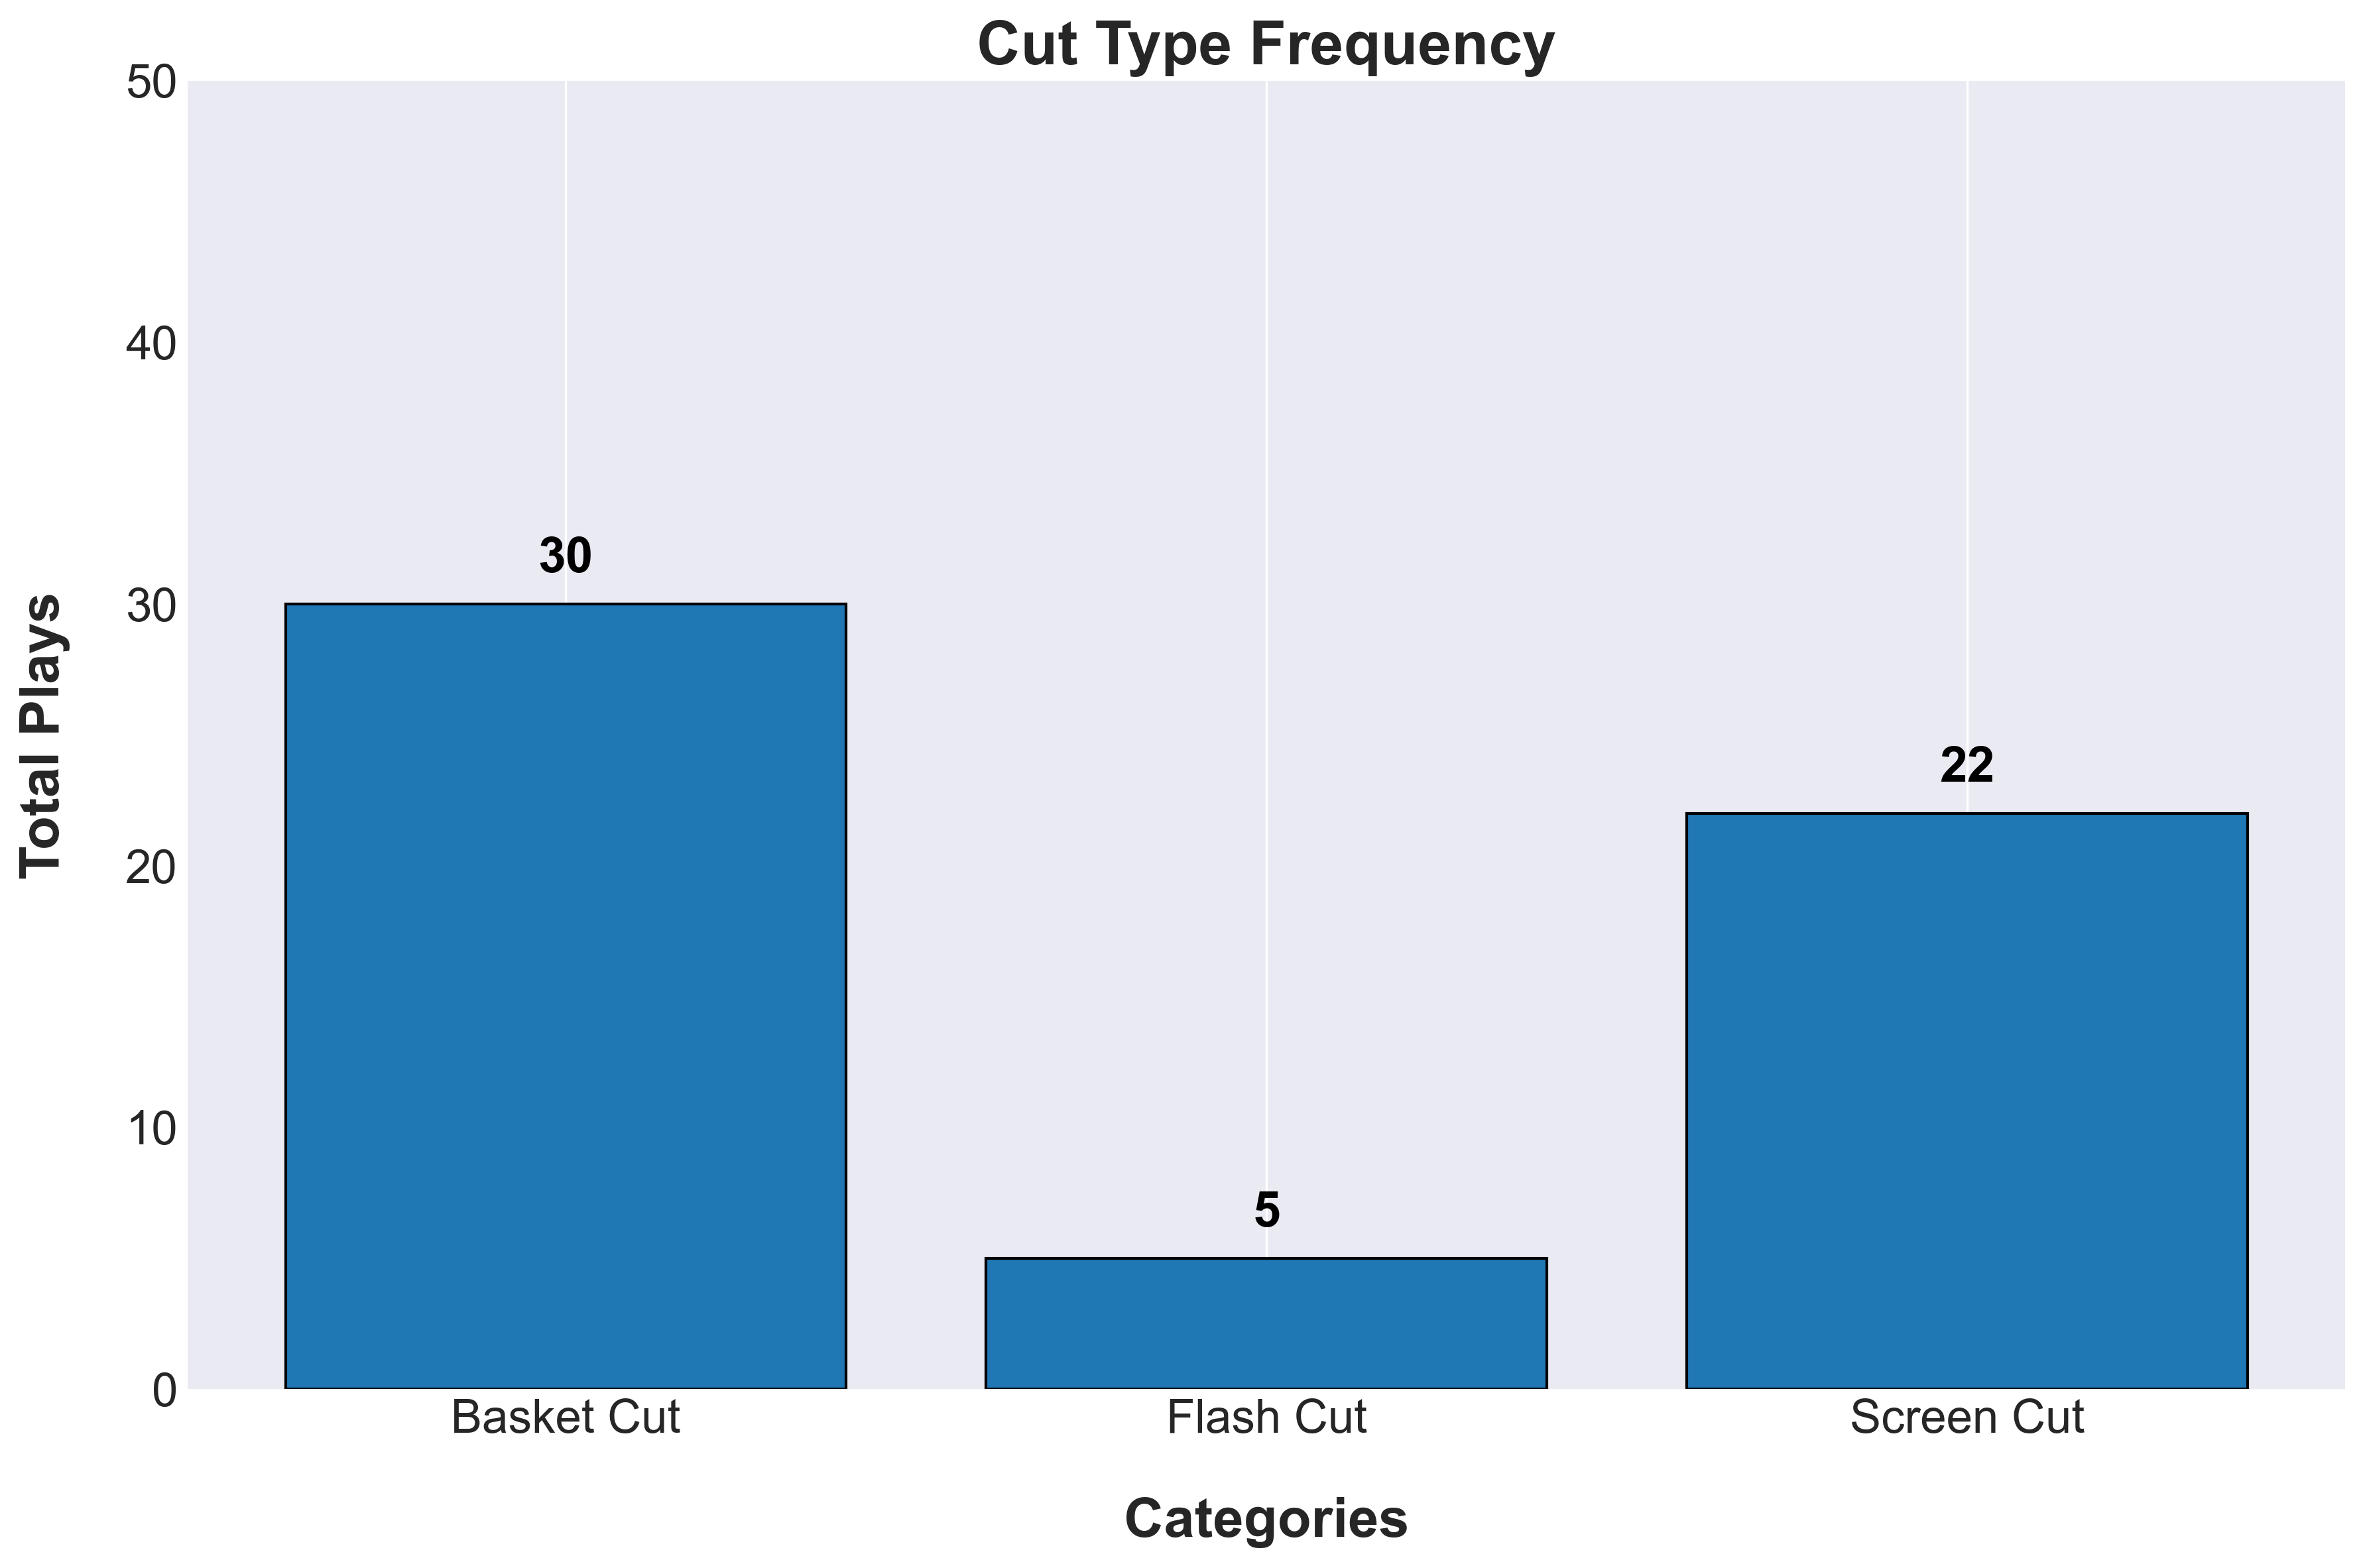
\includegraphics[width=\textwidth, height=.14\textheight]{images/Cut_Type_Freq.png} % Adjust the width of the image to fit
    \end{minipage}
\end{table}

\vspace{0em} % Add vertical space before the line (optional)
%\hrule height 1pt width 1\textwidth % Adjust height and width
\vspace{-1em} % Add vertical space after the line (optional)

\clearpage





% ----------------------
% PNR Visuals and Insights Section
% ----------------------
\subsection{Pick-and-Roll (PNR)}
\vspace{1.25em} % Add vertical space before the line (optional)
\textbf{Key Notes on PNR Tendencies}
\vspace{0.5em} % Add space between the title and the itemized list

\begin{itemize}
    \item PNR's make up x\% of players offensive load
    \vspace{0.3em} % Add space between the title and the itemized list
    \item Player is more efficient with rejecting screen and get shots off of rejecting screens x\% of the time.
\end{itemize}

\vspace{1em} % Add vertical space before the line (optional)
\hrule height 1pt width 1\textwidth % Adjust height and width
\vspace{0em} % Add vertical space after the line (optional)

\subsubsection{PNR Shot Statistics}

% All PNR Statistics Table w/ room for insights
\begin{table}[H]
    \centering
    \begin{minipage}[t]{0.6\textwidth} % Left side (table) takes 85% of the width
        %\flushright
        \centering % Centering the title and the table
        \text{Total Pick N Roll Shot Statistics} % Title above the table in bold
        \vskip .25em % Adds vertical space between title and table
        \scalebox{.85}{ % Scale the entire table down by half
            \scriptsize % Reduce the font size
            \begin{tabular}{
            >{\centering\arraybackslash}p{.75cm} 
            >{\centering\arraybackslash}p{.5cm} 
            >{\centering\arraybackslash}p{.5cm} 
            >{\centering\arraybackslash}p{.5cm}
            >{\centering\arraybackslash}p{.5cm} 
            >{\centering\arraybackslash}p{.5cm} 
            >{\centering\arraybackslash}p{.5cm} 
            >{\centering\arraybackslash}p{.5cm}
            >{\centering\arraybackslash}p{.5cm} 
            >{\centering\arraybackslash}p{.5cm}
            >{\centering\arraybackslash}p{.75cm}
            >{\centering\arraybackslash}p{.5cm} 
            >{\centering\arraybackslash}p{.5cm}}% Adjust column widths
            \toprule
            \textbf{Plays} &
            \textbf{3PA} &
            \textbf{3PM} &
            \textbf{3P\%} & 
            \textbf{2PA} & 
            \textbf{2PM} & 
            \textbf{2P\%} & 
            \textbf{MiA} & 
            \textbf{MiM} &
            \textbf{Mi\%} &
            \textbf{EFG\%} &
            \textbf{TO} &
            \textbf{Foul} \\
            \midrule
            
                
            
                
            
                
            
                
            
                
            
                
            
                
            
                
            
                
            
                
            
                
            
                
            
                
            
                
            
                
            
                
            
                
            
                
            
                
            
                
            
                
            
                
            
                
            
                
            
                
                    77 & 12 &
                    6 & - & 
                    44 & 17 &
                    - &
                    11 & 3 &
                    - &
                    - &
                    14 & 7 \\
                
            
                
            
                
            
                
            
                
            
                
            
                
            
                
            
                
            
                
            
                
            
                
            
                
            
                
            
            \bottomrule
            \end{tabular}
        }
    \end{minipage}
\end{table}

\vspace{0em} % Add vertical space before the line (optional)
%\hrule height 1pt width 1\textwidth % Adjust height and width
\vspace{-1em} % Add vertical space after the line (optional)

% PNR Stats for Rejecting vs Accepting Screens
\begin{table}[H]
    \raisebox{3em}{ % Adjust this value to shift the tables vertically
    \begin{minipage}[t]{0.6\textwidth} % Left side (table) takes 85% of the width
        \flushleft
        \centering % Centering the title and the table
        \text{PNR Usage Statistics} % Title above the table in bold
        \vskip .25em % Adds vertical space between title and table
        \scalebox{.6}{ % Scale the entire table down by half
            \renewcommand{\arraystretch}{1.4} % Adjust the number to increase or decrease row spacing
            \begin{tabular}{
            >{\centering\arraybackslash}p{1.75cm} 
            >{\centering\arraybackslash}p{.75cm} 
            >{\centering\arraybackslash}p{.75cm} 
            >{\centering\arraybackslash}p{.75cm} 
            >{\centering\arraybackslash}p{.75cm}
            >{\centering\arraybackslash}p{.75cm} 
            >{\centering\arraybackslash}p{.75cm} 
            >{\centering\arraybackslash}p{.75cm} 
            >{\centering\arraybackslash}p{.75cm}
            >{\centering\arraybackslash}p{.75cm} 
            >{\centering\arraybackslash}p{.75cm}
            >{\centering\arraybackslash}p{.75cm}
            >{\centering\arraybackslash}p{.75cm} 
            >{\centering\arraybackslash}p{.75cm}}% Adjust column widths
            \toprule
            {\scriptsize \textbf{PlayType}} &
            {\scriptsize \textbf{Plays}} &
            {\scriptsize \textbf{3PA}} &
            {\scriptsize \textbf{3PM}} &
            {\scriptsize \textbf{3P\%}} & 
            {\scriptsize \textbf{2PA}} & 
            {\scriptsize \textbf{2PM}} & 
            {\scriptsize \textbf{2P\%}} & 
            {\scriptsize \textbf{MiA}} & 
            {\scriptsize \textbf{MiM}} &
            {\scriptsize \textbf{Mi\%}} &
            {\scriptsize \textbf{EFG\%}} &
            {\scriptsize \textbf{TO}} &
            {\scriptsize \textbf{Foul}} \\
            \midrule
            
                
            
                
            
                
            
                
            
                
            
                
            
                
            
                
            
                
            
                
            
                
            
                
            
                
            
                
            
                
            
                
            
                
            
                
            
                
            
                
            
                
            
                
            
                
            
                
            
                
            
                
            
                
                    Accept & 56 & 6 & 3 &
                    - & 
                    34 & 13 &
                    - &
                    11 & 3 &
                    - &
                    - &
                    13 & 3 \\
                
            
                
                    Reject & 13 & 1 & 0 &
                    - & 
                    8 & 3 &
                    - &
                    0 & 0 &
                    - &
                    - &
                    1 & 3 \\
                
            
                
            
                
            
                
            
                
            
                
            
                
            
                
            
                
            
                
            
                
            

            \bottomrule
        \end{tabular}
        } % End of \scalebox
    \end{minipage}
    } % End of raisebox, closing the adjustment
    \hfill % This adds some flexible space between the table and the image
    \begin{minipage}[c]{0.35\textwidth} % Right side (image) takes 10% of the width
        \flushright
        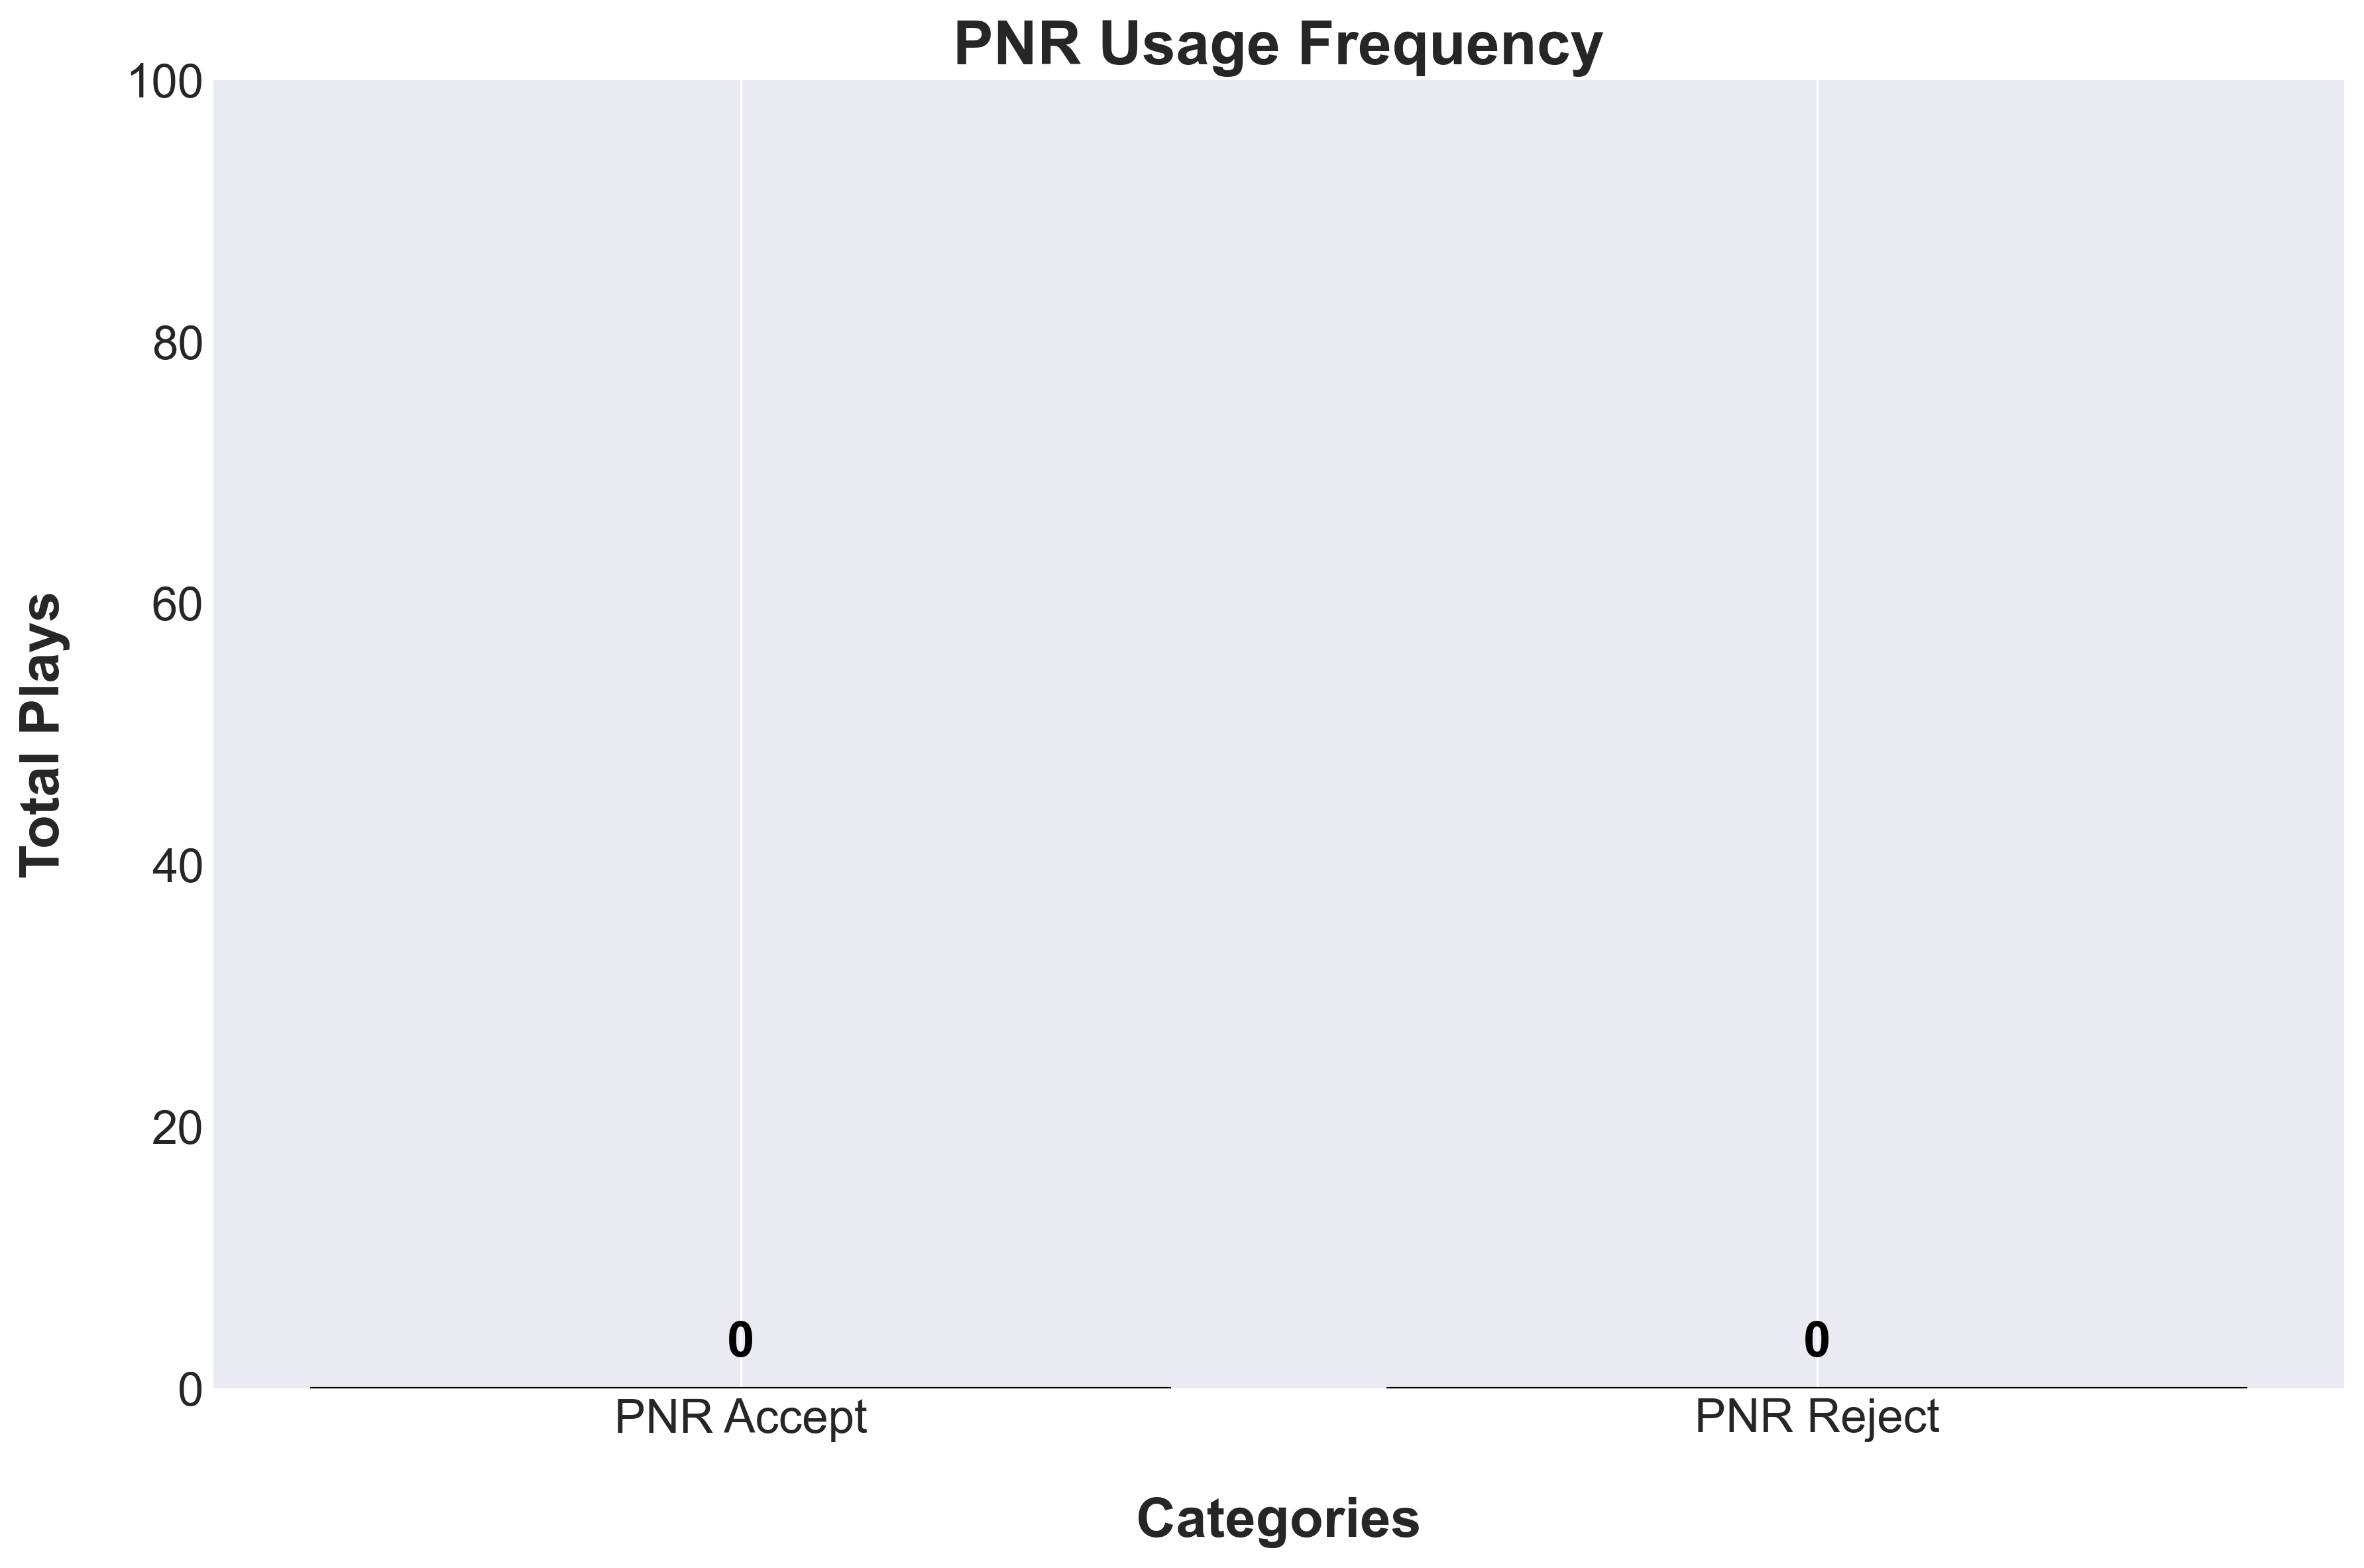
\includegraphics[width=\textwidth, height=.14\textheight]{images/PNR_Usage_Freq.png} % Adjust the width of the image to fit
    \end{minipage}
\end{table}

\vspace{-1em} % Add vertical space before the line (optional)
%\hrule height 1pt width 1\textwidth % Adjust height and width
\vspace{-1em} % Add vertical space after the line (optional)

% PNR Direction / Location Statistics
\begin{table}[H]
    \raisebox{3.5em}{ % Adjust this value to shift the tables vertically
    \begin{minipage}[t]{0.6\textwidth} % Left side (table) takes 85% of the width
        \flushleft
        \centering % Centering the title and the table
        \text{PNR Direction / Location Statistics} % Title above the table in bold
        \vskip .25em % Adds vertical space between title and table
        \scalebox{.6}{ % Scale the entire table down by half
            \renewcommand{\arraystretch}{1.4} % Adjust the number to increase or decrease row spacing
            \begin{tabular}{
            >{\centering\arraybackslash}p{1.75cm} 
            >{\centering\arraybackslash}p{.75cm} 
            >{\centering\arraybackslash}p{.75cm} 
            >{\centering\arraybackslash}p{.75cm} 
            >{\centering\arraybackslash}p{.75cm}
            >{\centering\arraybackslash}p{.75cm} 
            >{\centering\arraybackslash}p{.75cm} 
            >{\centering\arraybackslash}p{.75cm} 
            >{\centering\arraybackslash}p{.75cm}
            >{\centering\arraybackslash}p{.75cm} 
            >{\centering\arraybackslash}p{.75cm}
            >{\centering\arraybackslash}p{.75cm}
            >{\centering\arraybackslash}p{.75cm} 
            >{\centering\arraybackslash}p{.75cm}}% Adjust column widths
            \toprule
            {\scriptsize \textbf{PlayType}} &
            {\scriptsize \textbf{Plays}} &
            {\scriptsize \textbf{3PA}} &
            {\scriptsize \textbf{3PM}} &
            {\scriptsize \textbf{3P\%}} & 
            {\scriptsize \textbf{2PA}} & 
            {\scriptsize \textbf{2PM}} & 
            {\scriptsize \textbf{2P\%}} & 
            {\scriptsize \textbf{MiA}} & 
            {\scriptsize \textbf{MiM}} &
            {\scriptsize \textbf{Mi\%}} &
            {\scriptsize \textbf{EFG\%}} &
            {\scriptsize \textbf{TO}} &
            {\scriptsize \textbf{Foul}} \\
            \midrule
            
                
            
                
            
                
            
                
            
                
            
                
            
                
            
                
            
                
            
                
            
                
            
                
            
                
            
                
            
                
            
                
            
                
            
                
            
                
            
                
            
                
            
                
            
                
            
                
            
                
            
                
            
                
            
                
            
                
            
                
                    High & 41 & 7 & 3 &
                    - & 
                    23 & 11 &
                    - &
                    7 & 3 &
                    - &
                    - &
                    7 & 4 \\
                
            
                
                    Left & 16 & 2 & 2 &
                    - & 
                    11 & 4 &
                    - &
                    2 & 0 &
                    - &
                    - &
                    2 & 1 \\
                
            
                
                    Right & 20 & 3 & 1 &
                    - & 
                    10 & 2 &
                    - &
                    2 & 0 &
                    - &
                    - &
                    5 & 2 \\
                
            
                
            
                
            
                
            
                
            
                
            
                
            
            \bottomrule
        \end{tabular}
        } % End of \scalebox
    \end{minipage}
    } % End of raisebox, closing the adjustment
    \hfill
    \begin{minipage}[c]{0.35\textwidth} % Right side (image) takes 10% of the width
        \flushright
        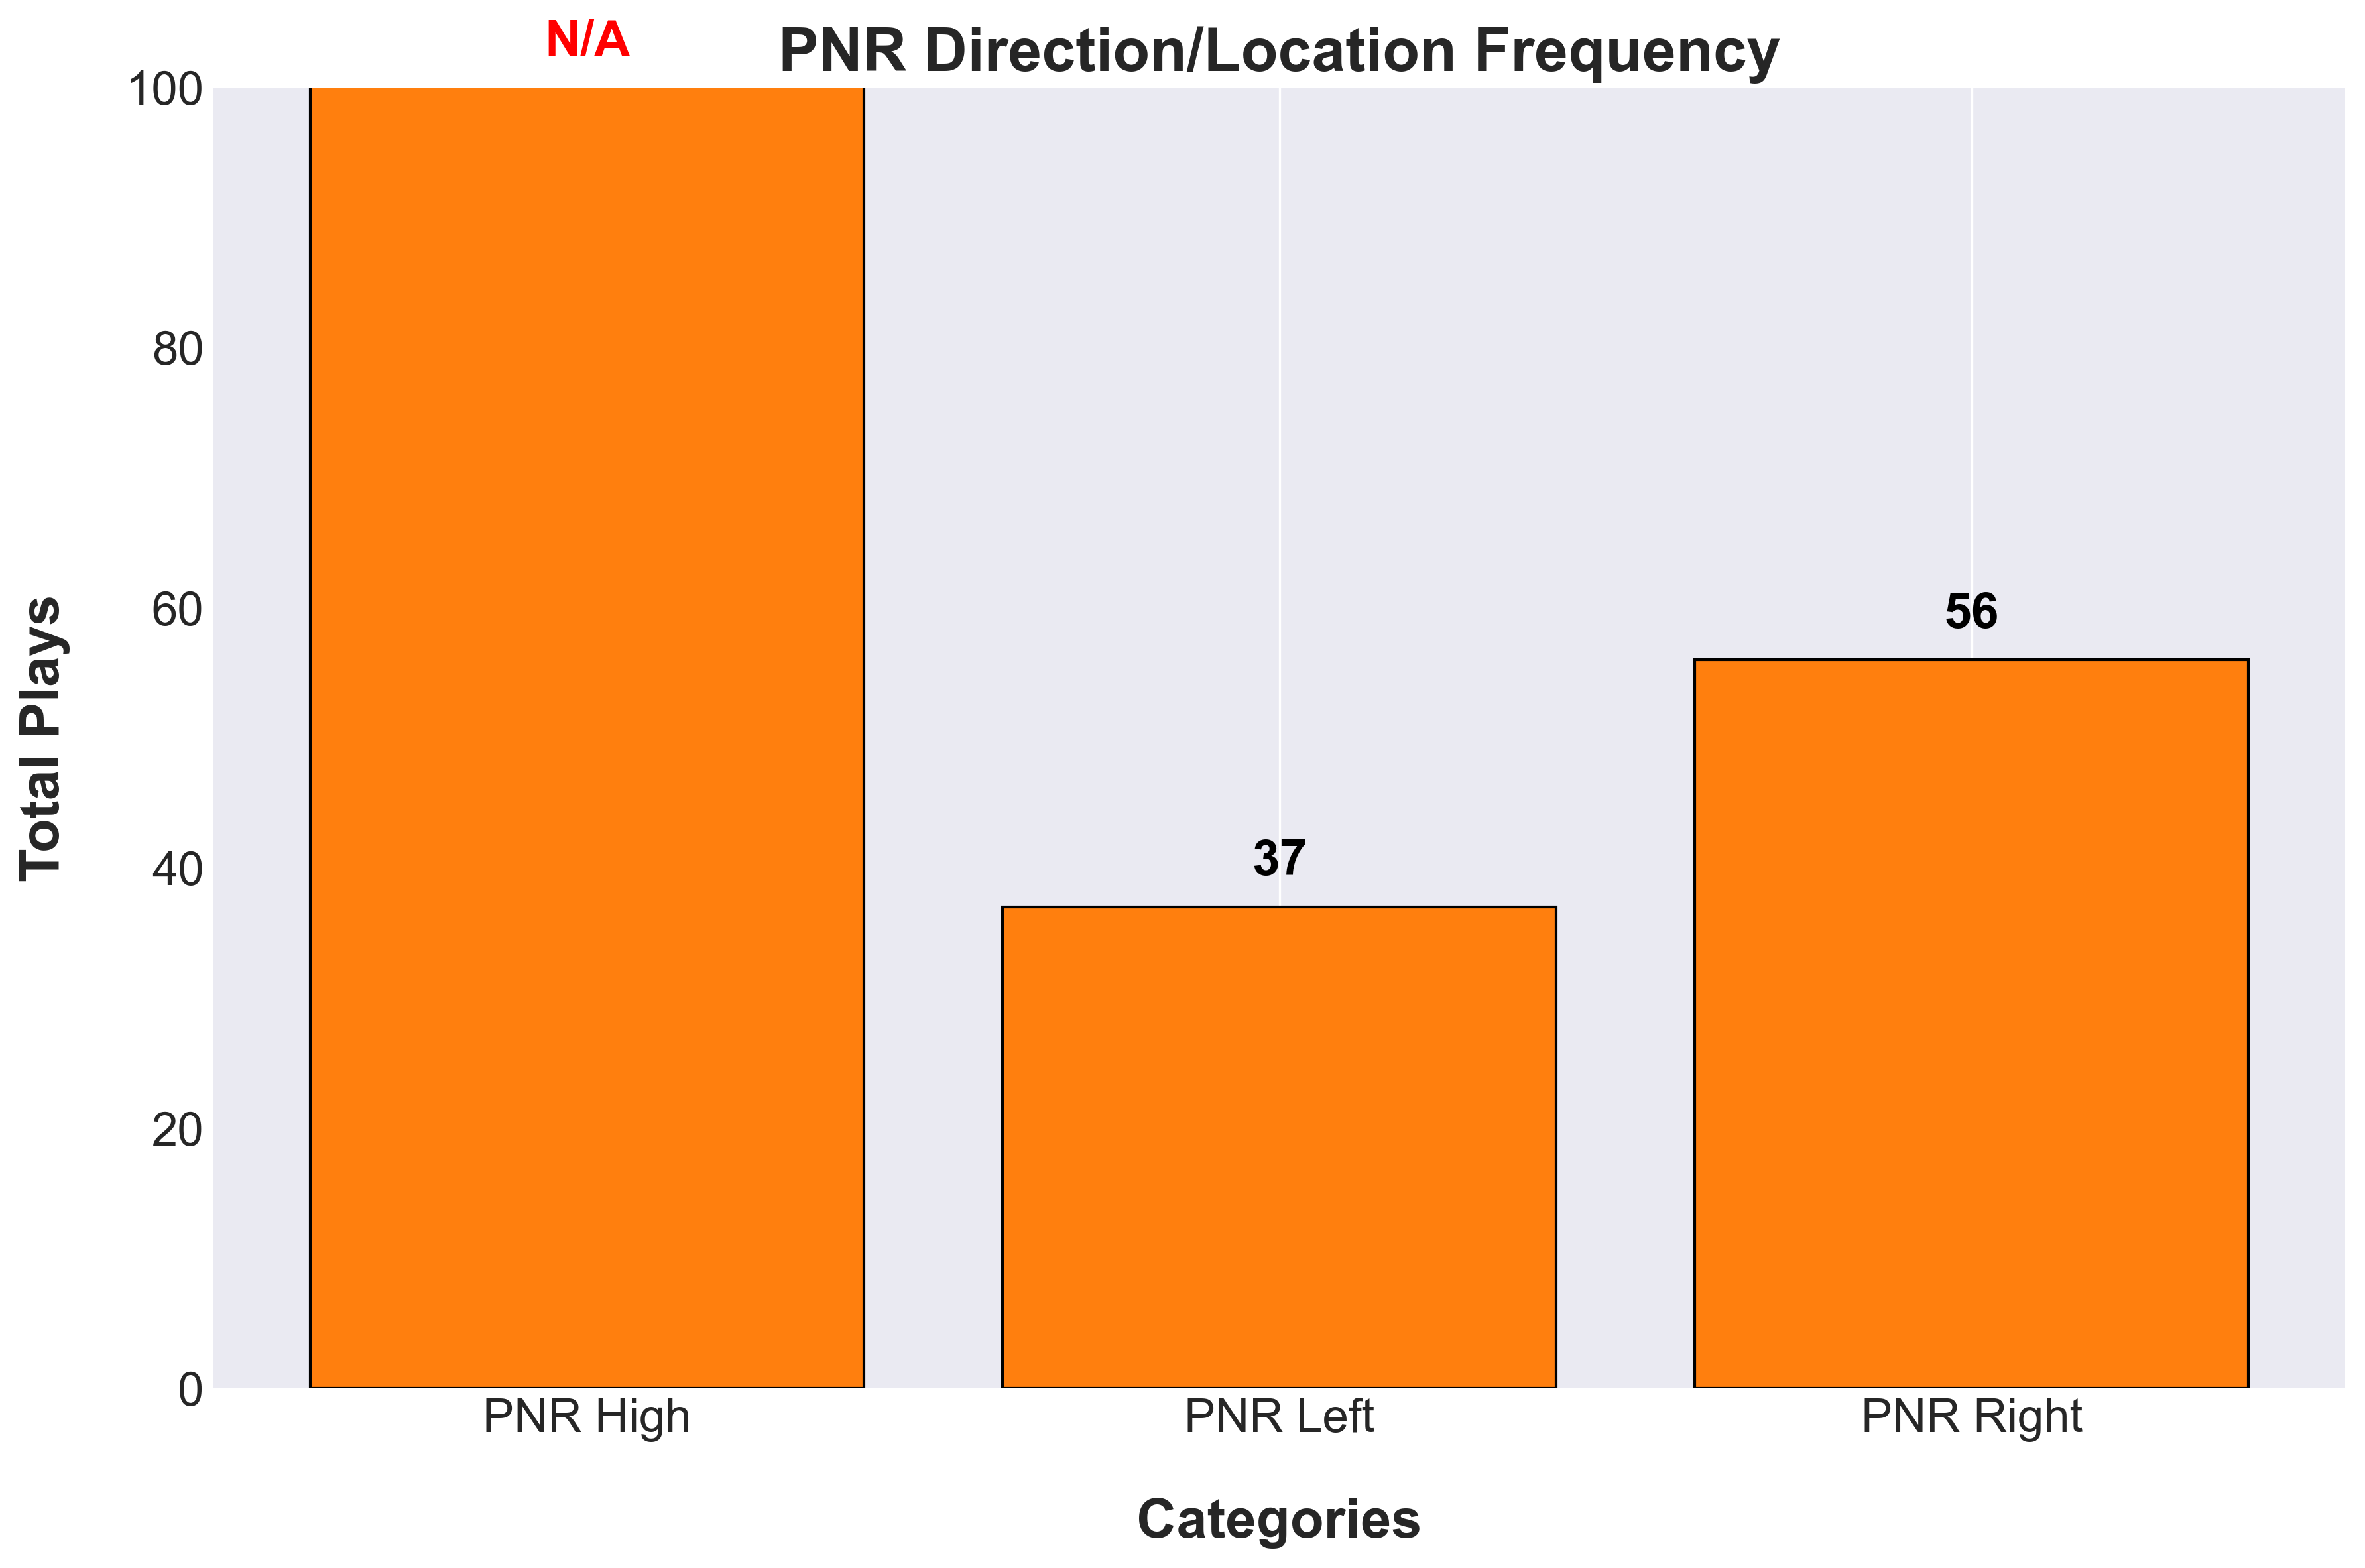
\includegraphics[width=\textwidth, height=.14\textheight]{images/PNR_DirectionLocation_Freq.png} % Adjust the width of the image to fit
    \end{minipage}
    
\end{table}

\vspace{-1em} % Add vertical space before the line (optional)
%\hrule height 1pt width 1\textwidth % Adjust height and width
\vspace{-1em} % Add vertical space after the line (optional)

% PNR Stats for Combination of Usage and Direction Stats
\begin{table}[H]
    \raisebox{4.5em}{ % Adjust this value to shift the tables vertically
    \begin{minipage}[t]{0.6\textwidth} % Left side (table) takes 85% of the width
        \flushleft
        \centering % Centering the title and the table
        \text{PNR Combination Statistics} % Title above the table in bold
        \vskip .25em % Adds vertical space between title and table
        \scalebox{.52}{ % Scale the entire table down by half
            \renewcommand{\arraystretch}{1.4} % Adjust the number to increase or decrease row spacing
            \begin{tabular}{
            >{\centering\arraybackslash}p{4cm} 
            >{\centering\arraybackslash}p{.75cm} 
            >{\centering\arraybackslash}p{.75cm} 
            >{\centering\arraybackslash}p{.75cm} 
            >{\centering\arraybackslash}p{.75cm}
            >{\centering\arraybackslash}p{.75cm} 
            >{\centering\arraybackslash}p{.75cm} 
            >{\centering\arraybackslash}p{.75cm} 
            >{\centering\arraybackslash}p{.75cm}
            >{\centering\arraybackslash}p{.75cm} 
            >{\centering\arraybackslash}p{.75cm}
            >{\centering\arraybackslash}p{.75cm}
            >{\centering\arraybackslash}p{.75cm} 
            >{\centering\arraybackslash}p{.75cm}}% Adjust column widths
            \toprule
            {\scriptsize \textbf{PlayType}} &
            {\scriptsize \textbf{Plays}} &
            {\scriptsize \textbf{3PA}} &
            {\scriptsize \textbf{3PM}} &
            {\scriptsize \textbf{3P\%}} & 
            {\scriptsize \textbf{2PA}} & 
            {\scriptsize \textbf{2PM}} & 
            {\scriptsize \textbf{2P\%}} & 
            {\scriptsize \textbf{MiA}} & 
            {\scriptsize \textbf{MiM}} &
            {\scriptsize \textbf{Mi\%}} &
            {\scriptsize \textbf{EFG\%}} &
            {\scriptsize \textbf{TO}} &
            {\scriptsize \textbf{Foul}} \\
            \midrule
            
                

            
                

            
                

            
                

            
                

            
                

            
                

            
                

            
                

            
                

            
                

            
                

            
                

            
                

            
                

            
                

            
                

            
                

            
                

            
                

            
                

            
                

            
                

            
                

            
                

            
                

            
                

            
                

            
                

            
                

            
                

            
                

            
                
                    High - Reject & 9 & 1 & 0 &
                    - & 
                    6 & 2 &
                    - &
                    0 & 0 &
                    - &
                    - &
                    0 & 2 \\
                

            
                
                High - Off & 30 & 4 & 3 &
                    - & 
                    17 & 9 &
                    - &
                    7 & 3 &
                    - &
                    - &
                    7 & 2 \\
                

            
                
                    Left - Reject & 2 & 0 & 0 &
                    - & 
                    1 & 0 &
                    - &
                    0 & 0 &
                    - &
                    - &
                    0 & 1 \\
                

            
                
                    Left - Off & 11 & 0 & 0 &
                    - & 
                    9 & 3 &
                    - &
                    2 & 0 &
                    - &
                    - &
                    2 & 0 \\
                

            
                
                    Right - Reject & 2 & 0 & 0 &
                    - & 
                    1 & 1 &
                    - &
                    0 & 0 &
                    - &
                    - &
                    1 & 0 \\
                

            
                
                    Right - Off & 15 & 2 & 0 &
                    - & 
                    8 & 1 &
                    - &
                    2 & 0 &
                    - &
                    - &
                    4 & 1 \\
                

            

            \bottomrule
        \end{tabular}
        } % End of \scalebox
    \end{minipage}
    } % End of raisebox, closing the adjustment
    \hfill % This adds some flexible space between the table and the image
    \begin{minipage}[c]{0.35\textwidth} % Right side (image) takes 10% of the width
        \flushright
        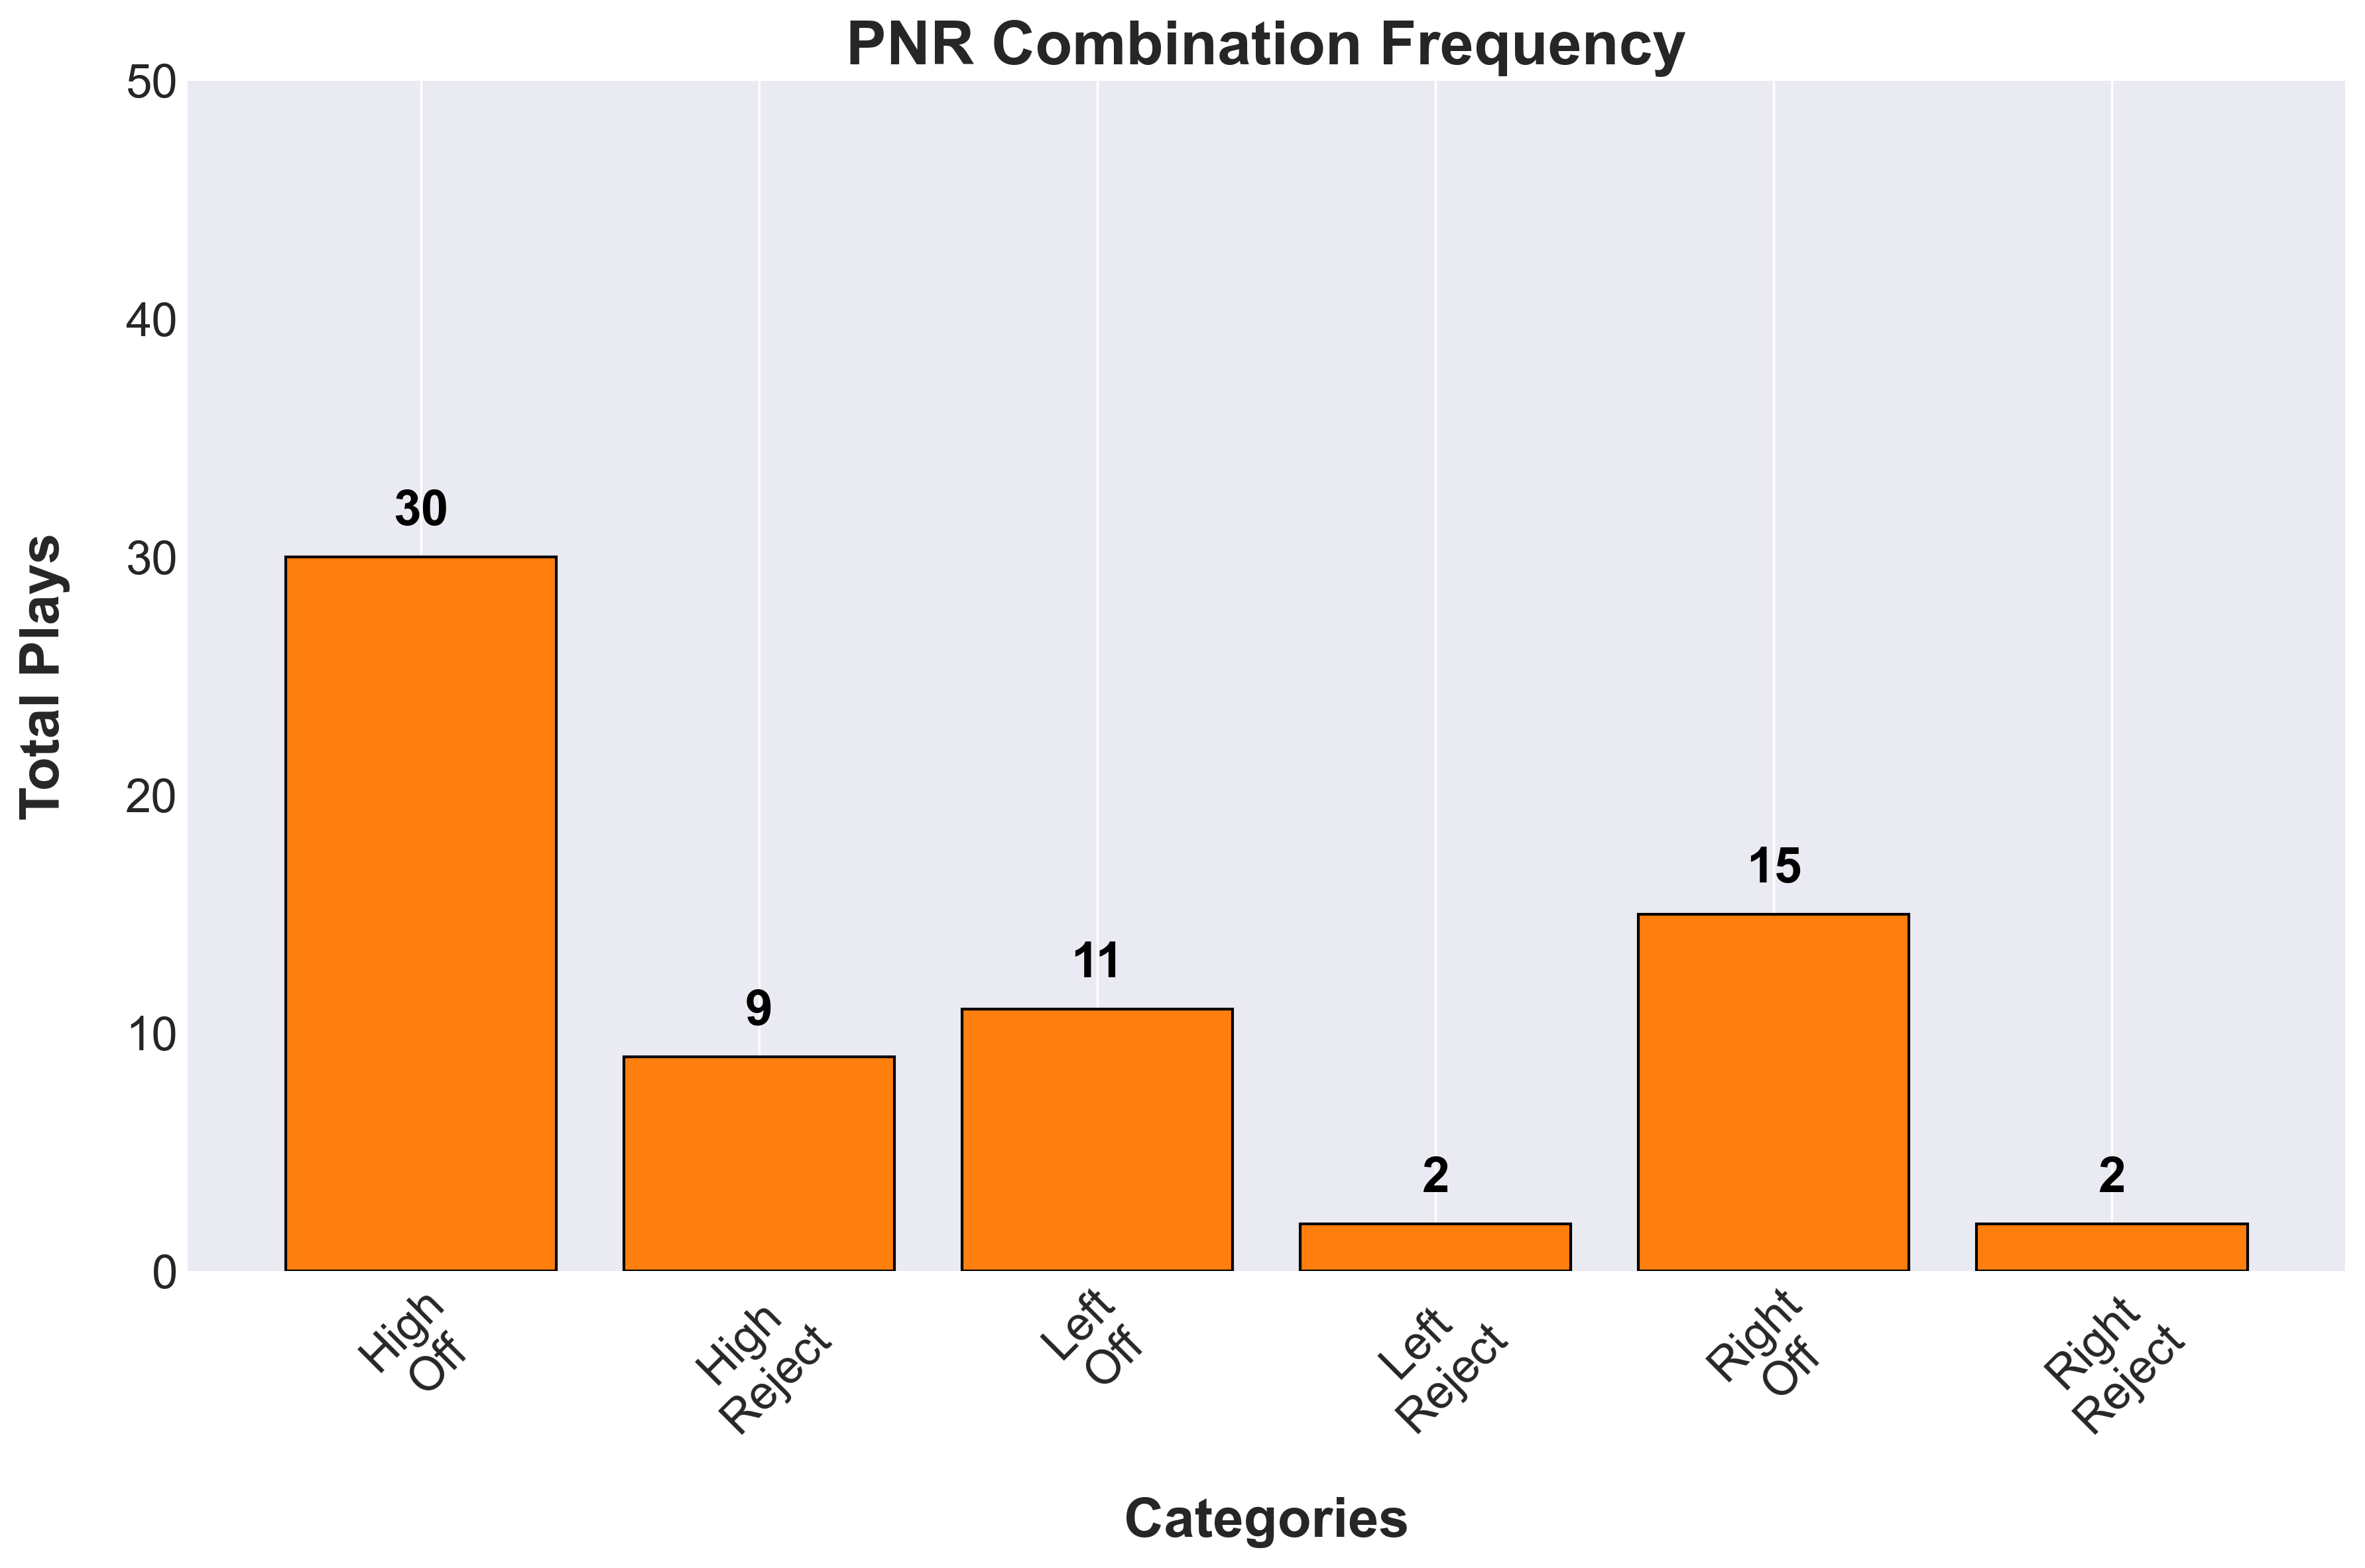
\includegraphics[width=\textwidth, height=.14\textheight]{images/PNR_Combination_Freq.png} % Adjust the width of the image to fit
    \end{minipage}
\end{table}

\vspace{-1em} % Add vertical space before the line (optional)
\hrule height 1pt width 1\textwidth % Adjust height and width
\vspace{1em} % Add vertical space after the line (optional)

\subsubsection{PNR Common Passer Statistics}

% All PNR Passer Statistics Table w/ room for insights
\begin{table}[H]
    \centering
    \begin{minipage}[t]{0.6\textwidth} % Left side (table) takes 85% of the width
        %\flushright
        \centering % Centering the title and the table
        \text{Total Pick N Roll Passer Statistics} % Title above the table in bold
        \vskip .25em % Adds vertical space between title and table
        \scalebox{.85}{ % Scale the entire table down by half
            \scriptsize % Reduce the font size
            \begin{tabular}{
            >{\centering\arraybackslash}p{.75cm} 
            >{\centering\arraybackslash}p{.5cm} 
            >{\centering\arraybackslash}p{.5cm} 
            >{\centering\arraybackslash}p{.5cm}
            >{\centering\arraybackslash}p{.5cm} 
            >{\centering\arraybackslash}p{.5cm} 
            >{\centering\arraybackslash}p{.5cm} 
            >{\centering\arraybackslash}p{.5cm}
            >{\centering\arraybackslash}p{.5cm} 
            >{\centering\arraybackslash}p{.5cm}
            >{\centering\arraybackslash}p{.75cm}
            >{\centering\arraybackslash}p{.5cm} 
            >{\centering\arraybackslash}p{.5cm}}% Adjust column widths
            \toprule
            \textbf{Plays} &
            \textbf{3PA} &
            \textbf{3PM} &
            \textbf{3P\%} & 
            \textbf{2PA} & 
            \textbf{2PM} & 
            \textbf{2P\%} & 
            \textbf{MiA} & 
            \textbf{MiM} &
            \textbf{Mi\%} &
            \textbf{EFG\%} &
            \textbf{TO} &
            \textbf{Foul} \\
            \midrule
            
                
            
                
                    70 & 37 & 9 &
                    - & 
                    24 & 13 &
                    - &
                    3 & 1 &
                    - &
                    - &
                    4 & 5 \\
                
            
                
            
                
            
                
            
                
            
                
            
                
            
                
            
                
            
                
            
                
            
                
            
                
            
                
            
                
            
                
            
                
            
                
            
                
            
                
            
                
            
                
            
                
            
                
            
                
            
                
            
                
            
                
            
                
            
                
            
                
            
                
            
                
            
                
            
                
            
                
            
                
            
            \bottomrule
            \end{tabular}
        }
    \end{minipage}
\end{table}

\vspace{-1em} % Add vertical space before the line (optional)
%\hrule height 1pt width 1\textwidth % Adjust height and width
\vspace{0em} % Add vertical space after the line (optional)

% PNR -> Different PlayType Statistics
\begin{table}[H]
    \raisebox{3em}{ % Adjust this value to shift the tables vertically
    \begin{minipage}[t]{0.6\textwidth} % Left side (table) takes 85% of the width
        \flushleft
        \centering % Centering the title and the table
        \text{PNR to Different PlayType Statistics} % Title above the table in bold
        \vskip .25em % Adds vertical space between title and table
        \scalebox{.6}{ % Scale the entire table
            \scriptsize % Reduce the font size
            \renewcommand{\arraystretch}{1.3} % Adjust the number to increase or decrease row spacing
            \begin{tabular}{
            >{\centering\arraybackslash}p{1.5cm} 
            >{\centering\arraybackslash}p{.75cm} 
            >{\centering\arraybackslash}p{.75cm} 
            >{\centering\arraybackslash}p{.75cm} 
            >{\centering\arraybackslash}p{.75cm}
            >{\centering\arraybackslash}p{.75cm} 
            >{\centering\arraybackslash}p{.75cm} 
            >{\centering\arraybackslash}p{.75cm} 
            >{\centering\arraybackslash}p{.75cm}
            >{\centering\arraybackslash}p{.75cm} 
            >{\centering\arraybackslash}p{.75cm}
            >{\centering\arraybackslash}p{.75cm}
            >{\centering\arraybackslash}p{.75cm} 
            >{\centering\arraybackslash}p{.75cm}}% Adjust column widths
            \toprule
            {\scriptsize \textbf{PlayType}} &
            {\scriptsize \textbf{Plays}} &
            {\scriptsize \textbf{3PA}} &
            {\scriptsize \textbf{3PM}} &
            {\scriptsize \textbf{3P\%}} & 
            {\scriptsize \textbf{2PA}} & 
            {\scriptsize \textbf{2PM}} & 
            {\scriptsize \textbf{2P\%}} & 
            {\scriptsize \textbf{MiA}} & 
            {\scriptsize \textbf{MiM}} &
            {\scriptsize \textbf{Mi\%}} &
            {\scriptsize \textbf{EFG\%}} &
            {\scriptsize \textbf{TO}} &
            {\scriptsize \textbf{Foul}} \\
            \midrule
            
                
            
                
            
                
                    Cuts & 5 & 0 & 0 &
                    - & 
                    4 & 4 &
                    - &
                    0 & 0 &
                    - &
                    - &
                    0 & 1 \\
                
            
                
                    S.U Drives & 15 & 3 & 0 &
                    - & 
                    6 & 3 &
                    - &
                    0 & 0 &
                    - &
                    - &
                    4 & 2 \\
                
            
                
                    S.U Shots & 30 & 28 & 8 &
                    - & 
                    2 & 0 &
                    - &
                    2 & 0 &
                    - &
                    - &
                    0 & 0 \\
                
            
                
                    Rollman & 20 & 6 & 1 &
                    - & 
                    12 & 6 &
                    - &
                    1 & 1 &
                    - &
                    - &
                    0 & 2 \\
                
            
                
            
                
            
                
            
                
            
                
            
                
            
                
            
                
            
                
            
                
            
                
            
                
            
                
            
                
            
                
            
                
            
                
            
                
            
                
            
                
            
                
            
                
            
                
            
                
            
                
            
                
            
                
            
                
            
                
            
                
            
                
            
                
            

            \bottomrule
        \end{tabular}
        }
    \end{minipage}
    }
    \hfill % This adds some flexible space between the table and the image
    \begin{minipage}[c]{0.35\textwidth} % Right side (image) takes 10% of the width
        \flushright
        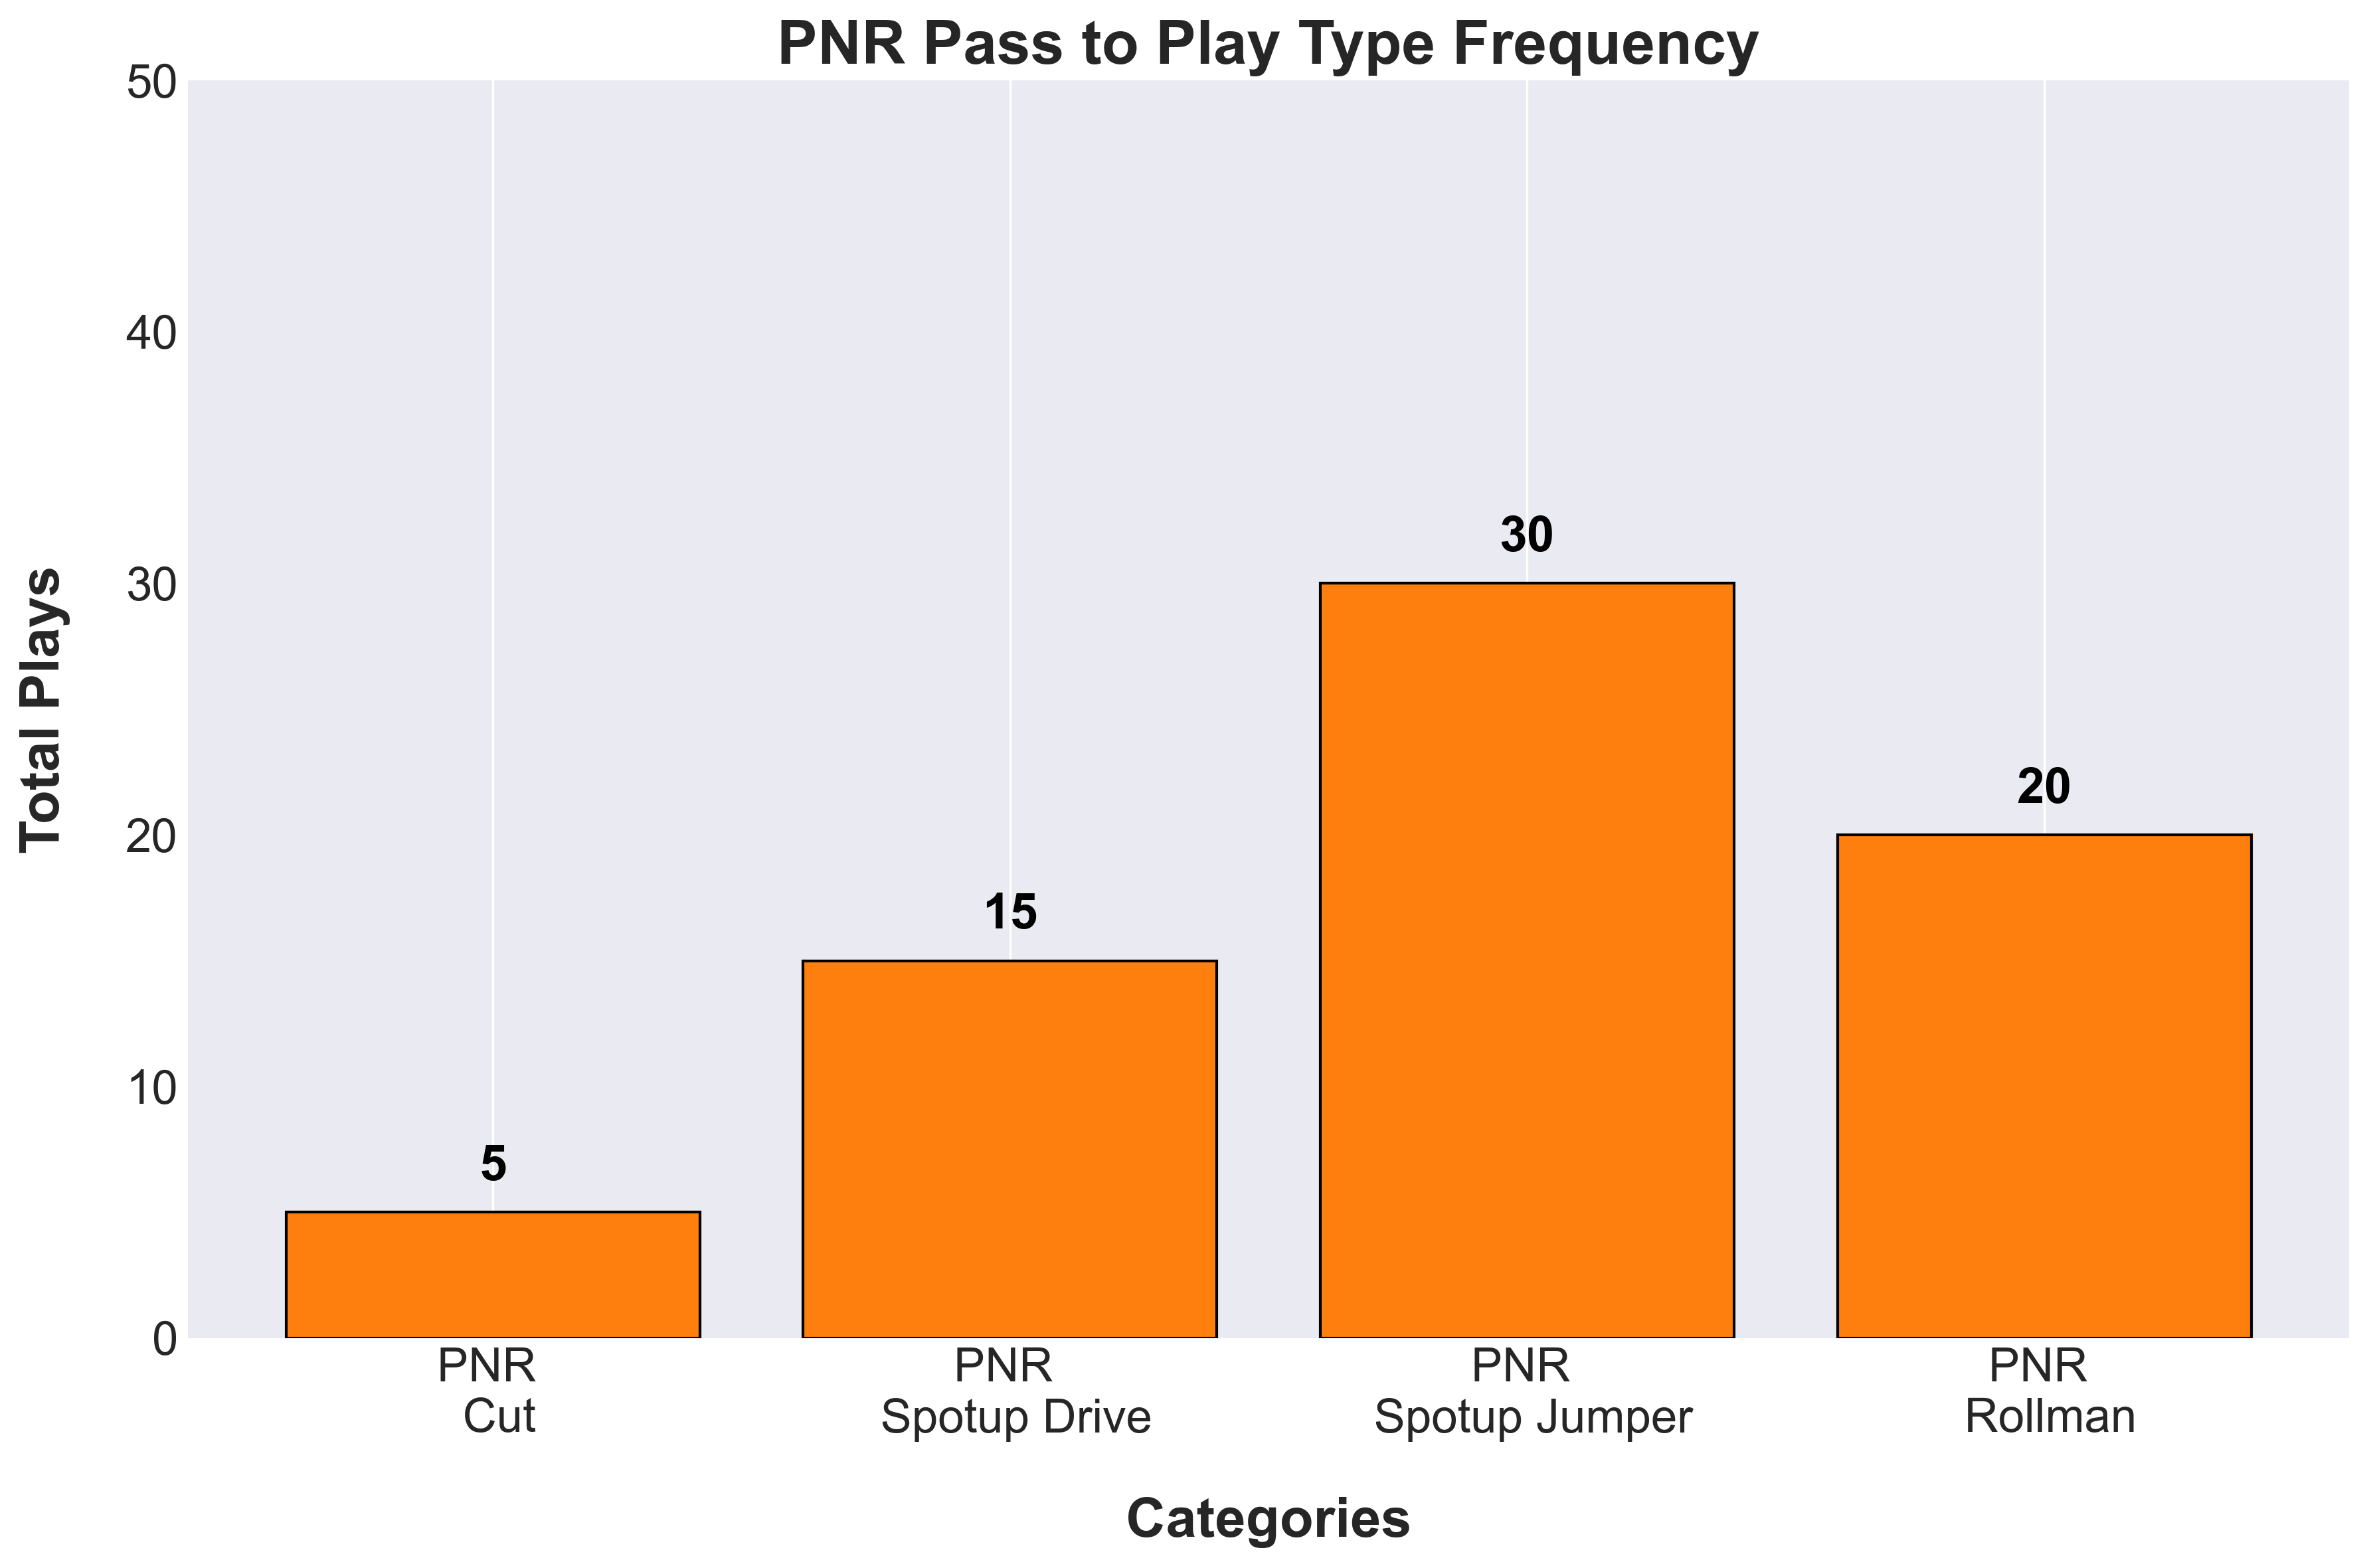
\includegraphics[width=\textwidth, height=.14\textheight]{images/PNR_PassPlayType_Freq.png} % Adjust the width of the image to fit
    \end{minipage}
\end{table}

\vspace{-1em} % Add vertical space before the line (optional)
\hrule height 1pt width 1\textwidth % Adjust height and width
\vspace{1em} % Add vertical space after the line (optional)

\subsubsection{BH High PNR Passer Statistics}

% BH High -> Cuts Secondary Player Stats
\begin{table}[H]
    \raisebox{3em}{ % Adjust this value to shift the tables vertically
    \begin{minipage}[t]{0.6\textwidth} % Left side (table) takes 85% of the width
        \flushleft
        \centering % Centering the title and the table
        \text{BH High - Cuts Player Statistics} % Title above the table in bold
        \vskip .25em % Adds vertical space between title and table
        \scalebox{.6}{ % Scale the entire table down by half
            \renewcommand{\arraystretch}{1.4} % Adjust the number to increase or decrease row spacing
            \begin{tabular}{
            >{\centering\arraybackslash}p{3cm} 
            >{\centering\arraybackslash}p{.75cm} 
            >{\centering\arraybackslash}p{.75cm} 
            >{\centering\arraybackslash}p{.75cm} 
            >{\centering\arraybackslash}p{.75cm}
            >{\centering\arraybackslash}p{.75cm} 
            >{\centering\arraybackslash}p{.75cm}
            >{\centering\arraybackslash}p{.75cm}
            >{\centering\arraybackslash}p{.75cm} 
            >{\centering\arraybackslash}p{.75cm}}% Adjust column widths
            \toprule
            {\scriptsize \textbf{Player}} &
            {\scriptsize \textbf{Plays}} &
            {\scriptsize \textbf{2PA}} & 
            {\scriptsize \textbf{2PM}} & 
            {\scriptsize \textbf{2P\%}} & 
            {\scriptsize \textbf{MiA}} & 
            {\scriptsize \textbf{MiM}} &
            {\scriptsize \textbf{Mi\%}} &
            {\scriptsize \textbf{TO}} &
            {\scriptsize \textbf{Foul}} \\
            \midrule
            
                
            
                
            
                
            
                
            
                
            
                
            
                
                    
                        Keegan Ocorr & 
                        2 & 
                        1 & 
                        1 & 
                        - & 
                        0 & 
                        0 & 
                        - & 
                        0 & 
                        1 \\
                    
                        Luke Granto & 
                        1 & 
                        1 & 
                        1 & 
                        - & 
                        0 & 
                        0 & 
                        - & 
                        0 & 
                        0 \\
                    
                        Zac Ditzel & 
                        1 & 
                        1 & 
                        1 & 
                        - & 
                        0 & 
                        0 & 
                        - & 
                        0 & 
                        0 \\
                    
                
            
                
            
                
            
                
            
                
            
                
            
                
            
                
            
                
            
                
            
                
            
                
            
                
            
                
            
                
            
                
            
                
            
                
            
                
            
                
            
                
            
                
            
                
            
                
            
                
            
                
            
                
            
                
            
                
            
                
            
                
            
                
            
            \bottomrule
        \end{tabular}
        } % End of \scalebox
    \end{minipage}
    } % End of raisebox, closing the adjustment
    \hfill % This adds some flexible space between the table and the image
    \begin{minipage}[c]{0.35\textwidth} % Right side (image) takes 10% of the width
        \flushright
        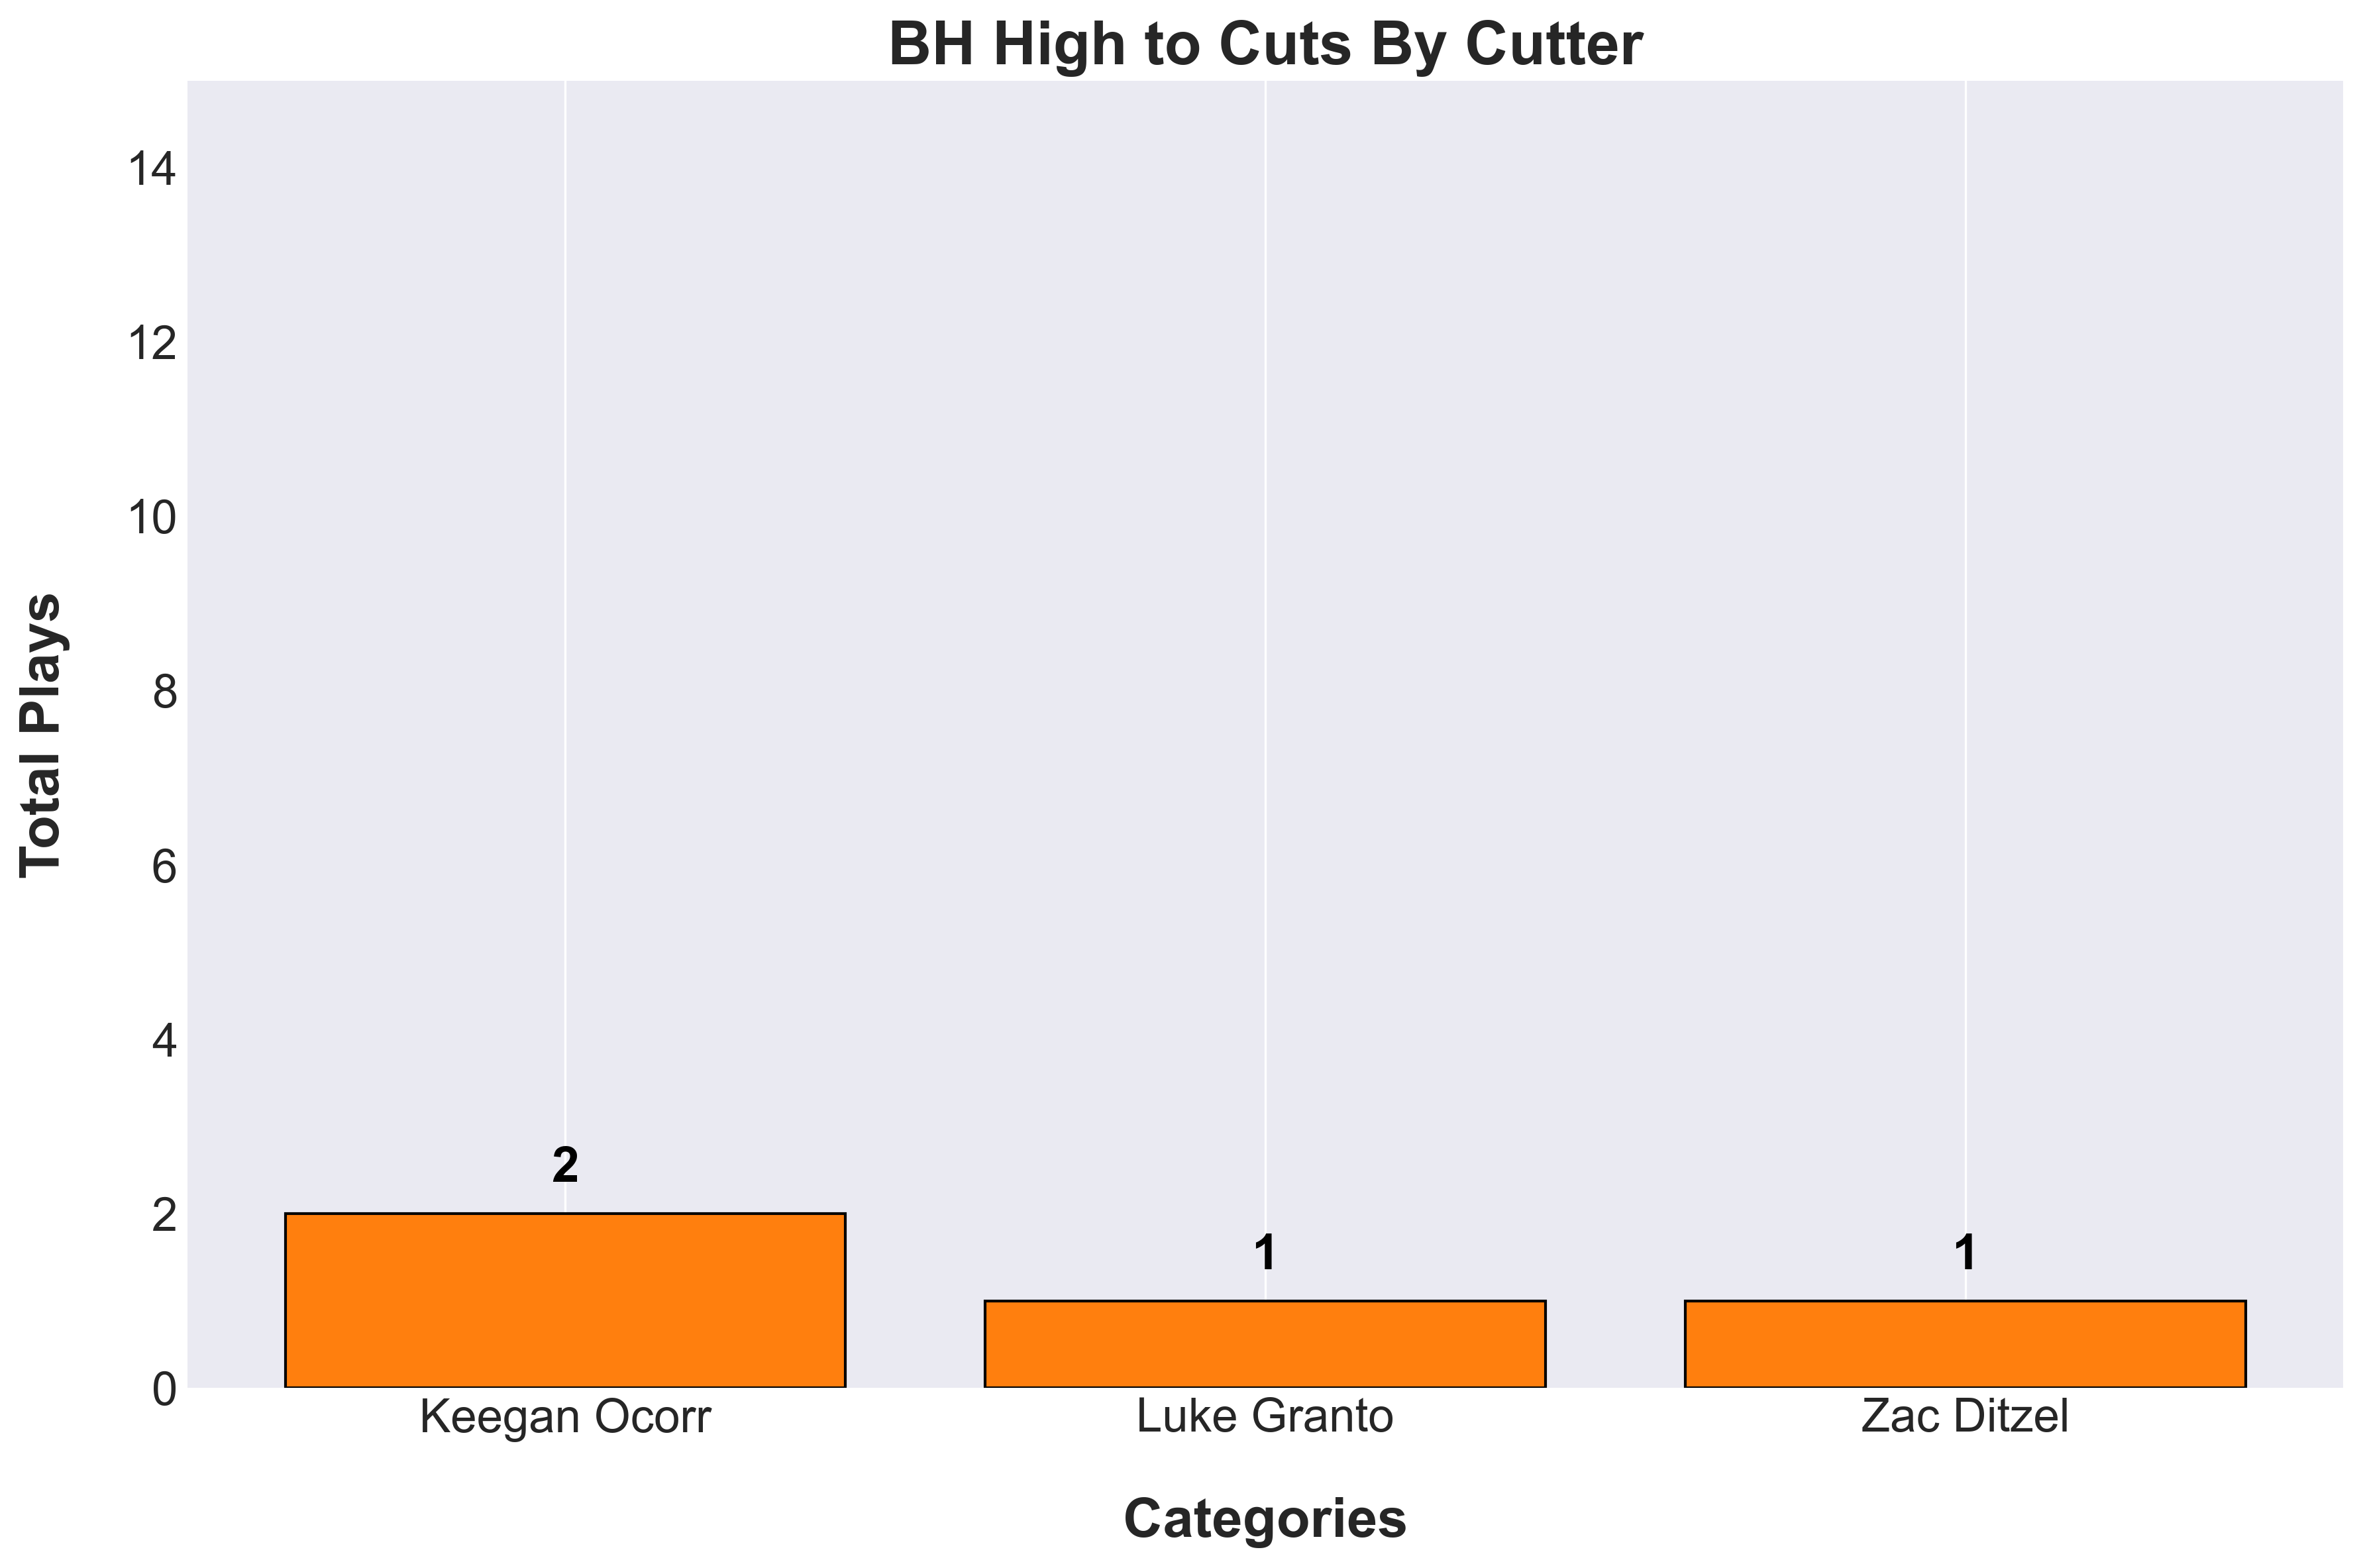
\includegraphics[width=\textwidth, height=.14\textheight]{images/PNR_PassHighCutsPlayer_Freq.png} % Adjust the width of the image to fit
    \end{minipage}
\end{table}

\vspace{-1em} % Add vertical space before the line (optional)
%\hrule height 1pt width 1\textwidth % Adjust height and width
\vspace{-1em} % Add vertical space after the line (optional)

% BH High -> Spot Up Drives Secondary Player Stats
\begin{table}[H]
    \raisebox{3em}{ % Adjust this value to shift the tables vertically
    \begin{minipage}[t]{0.6\textwidth} % Left side (table) takes 85% of the width
        \flushleft
        \centering % Centering the title and the table
        \text{BH High - Spot Up Drives Player Statistics} % Title above the table in bold
        \vskip .25em % Adds vertical space between title and table
        \scalebox{.55}{ % Scale the entire table down by half
            \renewcommand{\arraystretch}{1.4} % Adjust the number to increase or decrease row spacing
            \begin{tabular}{
            >{\centering\arraybackslash}p{3cm} 
            >{\centering\arraybackslash}p{.75cm} 
            >{\centering\arraybackslash}p{.75cm} 
            >{\centering\arraybackslash}p{.75cm} 
            >{\centering\arraybackslash}p{.75cm}
            >{\centering\arraybackslash}p{.75cm} 
            >{\centering\arraybackslash}p{.75cm} 
            >{\centering\arraybackslash}p{.75cm} 
            >{\centering\arraybackslash}p{.75cm}
            >{\centering\arraybackslash}p{.75cm} 
            >{\centering\arraybackslash}p{.75cm}
            >{\centering\arraybackslash}p{.75cm}
            >{\centering\arraybackslash}p{.75cm} 
            >{\centering\arraybackslash}p{.75cm}}% Adjust column widths
            \toprule
            {\scriptsize \textbf{Player}} &
            {\scriptsize \textbf{Plays}} &
            {\scriptsize \textbf{3PA}} &
            {\scriptsize \textbf{3PM}} &
            {\scriptsize \textbf{3P\%}} & 
            {\scriptsize \textbf{2PA}} & 
            {\scriptsize \textbf{2PM}} & 
            {\scriptsize \textbf{2P\%}} & 
            {\scriptsize \textbf{MiA}} & 
            {\scriptsize \textbf{MiM}} &
            {\scriptsize \textbf{Mi\%}} &
            {\scriptsize \textbf{EFG\%}} &
            {\scriptsize \textbf{TO}} &
            {\scriptsize \textbf{Foul}} \\
            \midrule
            
                
            
                
            
                
            
                
            
                
            
                
            
                
            
                
                    
                        Brock Bowen & 
                        2 & 
                        1 & 
                        0 & 
                        - & 
                        1 & 
                        1 & 
                        - & 
                        0 & 
                        0 & 
                        - & 
                        - & 
                        0 & 
                        0 \\
                    
                        Brody Brown & 
                        1 & 
                        0 & 
                        0 & 
                        - & 
                        0 & 
                        0 & 
                        - & 
                        0 & 
                        0 & 
                        - & 
                        - & 
                        1 & 
                        0 \\
                    
                        Keegan Ocorr & 
                        4 & 
                        0 & 
                        0 & 
                        - & 
                        1 & 
                        1 & 
                        - & 
                        0 & 
                        0 & 
                        - & 
                        - & 
                        2 & 
                        1 \\
                    
                        Mark Osime & 
                        1 & 
                        0 & 
                        0 & 
                        - & 
                        1 & 
                        0 & 
                        - & 
                        0 & 
                        0 & 
                        - & 
                        - & 
                        0 & 
                        0 \\
                    
                        Zac Ditzel & 
                        2 & 
                        1 & 
                        0 & 
                        - & 
                        1 & 
                        1 & 
                        - & 
                        0 & 
                        0 & 
                        - & 
                        - & 
                        0 & 
                        0 \\
                    
                
            
                
            
                
            
                
            
                
            
                
            
                
            
                
            
                
            
                
            
                
            
                
            
                
            
                
            
                
            
                
            
                
            
                
            
                
            
                
            
                
            
                
            
                
            
                
            
                
            
                
            
                
            
                
            
                
            
                
            
                
            

            \bottomrule
        \end{tabular}
        } % End of \scalebox
    \end{minipage}
    } % End of raisebox, closing the adjustment
    \hfill % This adds some flexible space between the table and the image
    \begin{minipage}[c]{0.35\textwidth} % Right side (image) takes 10% of the width
        \flushright
        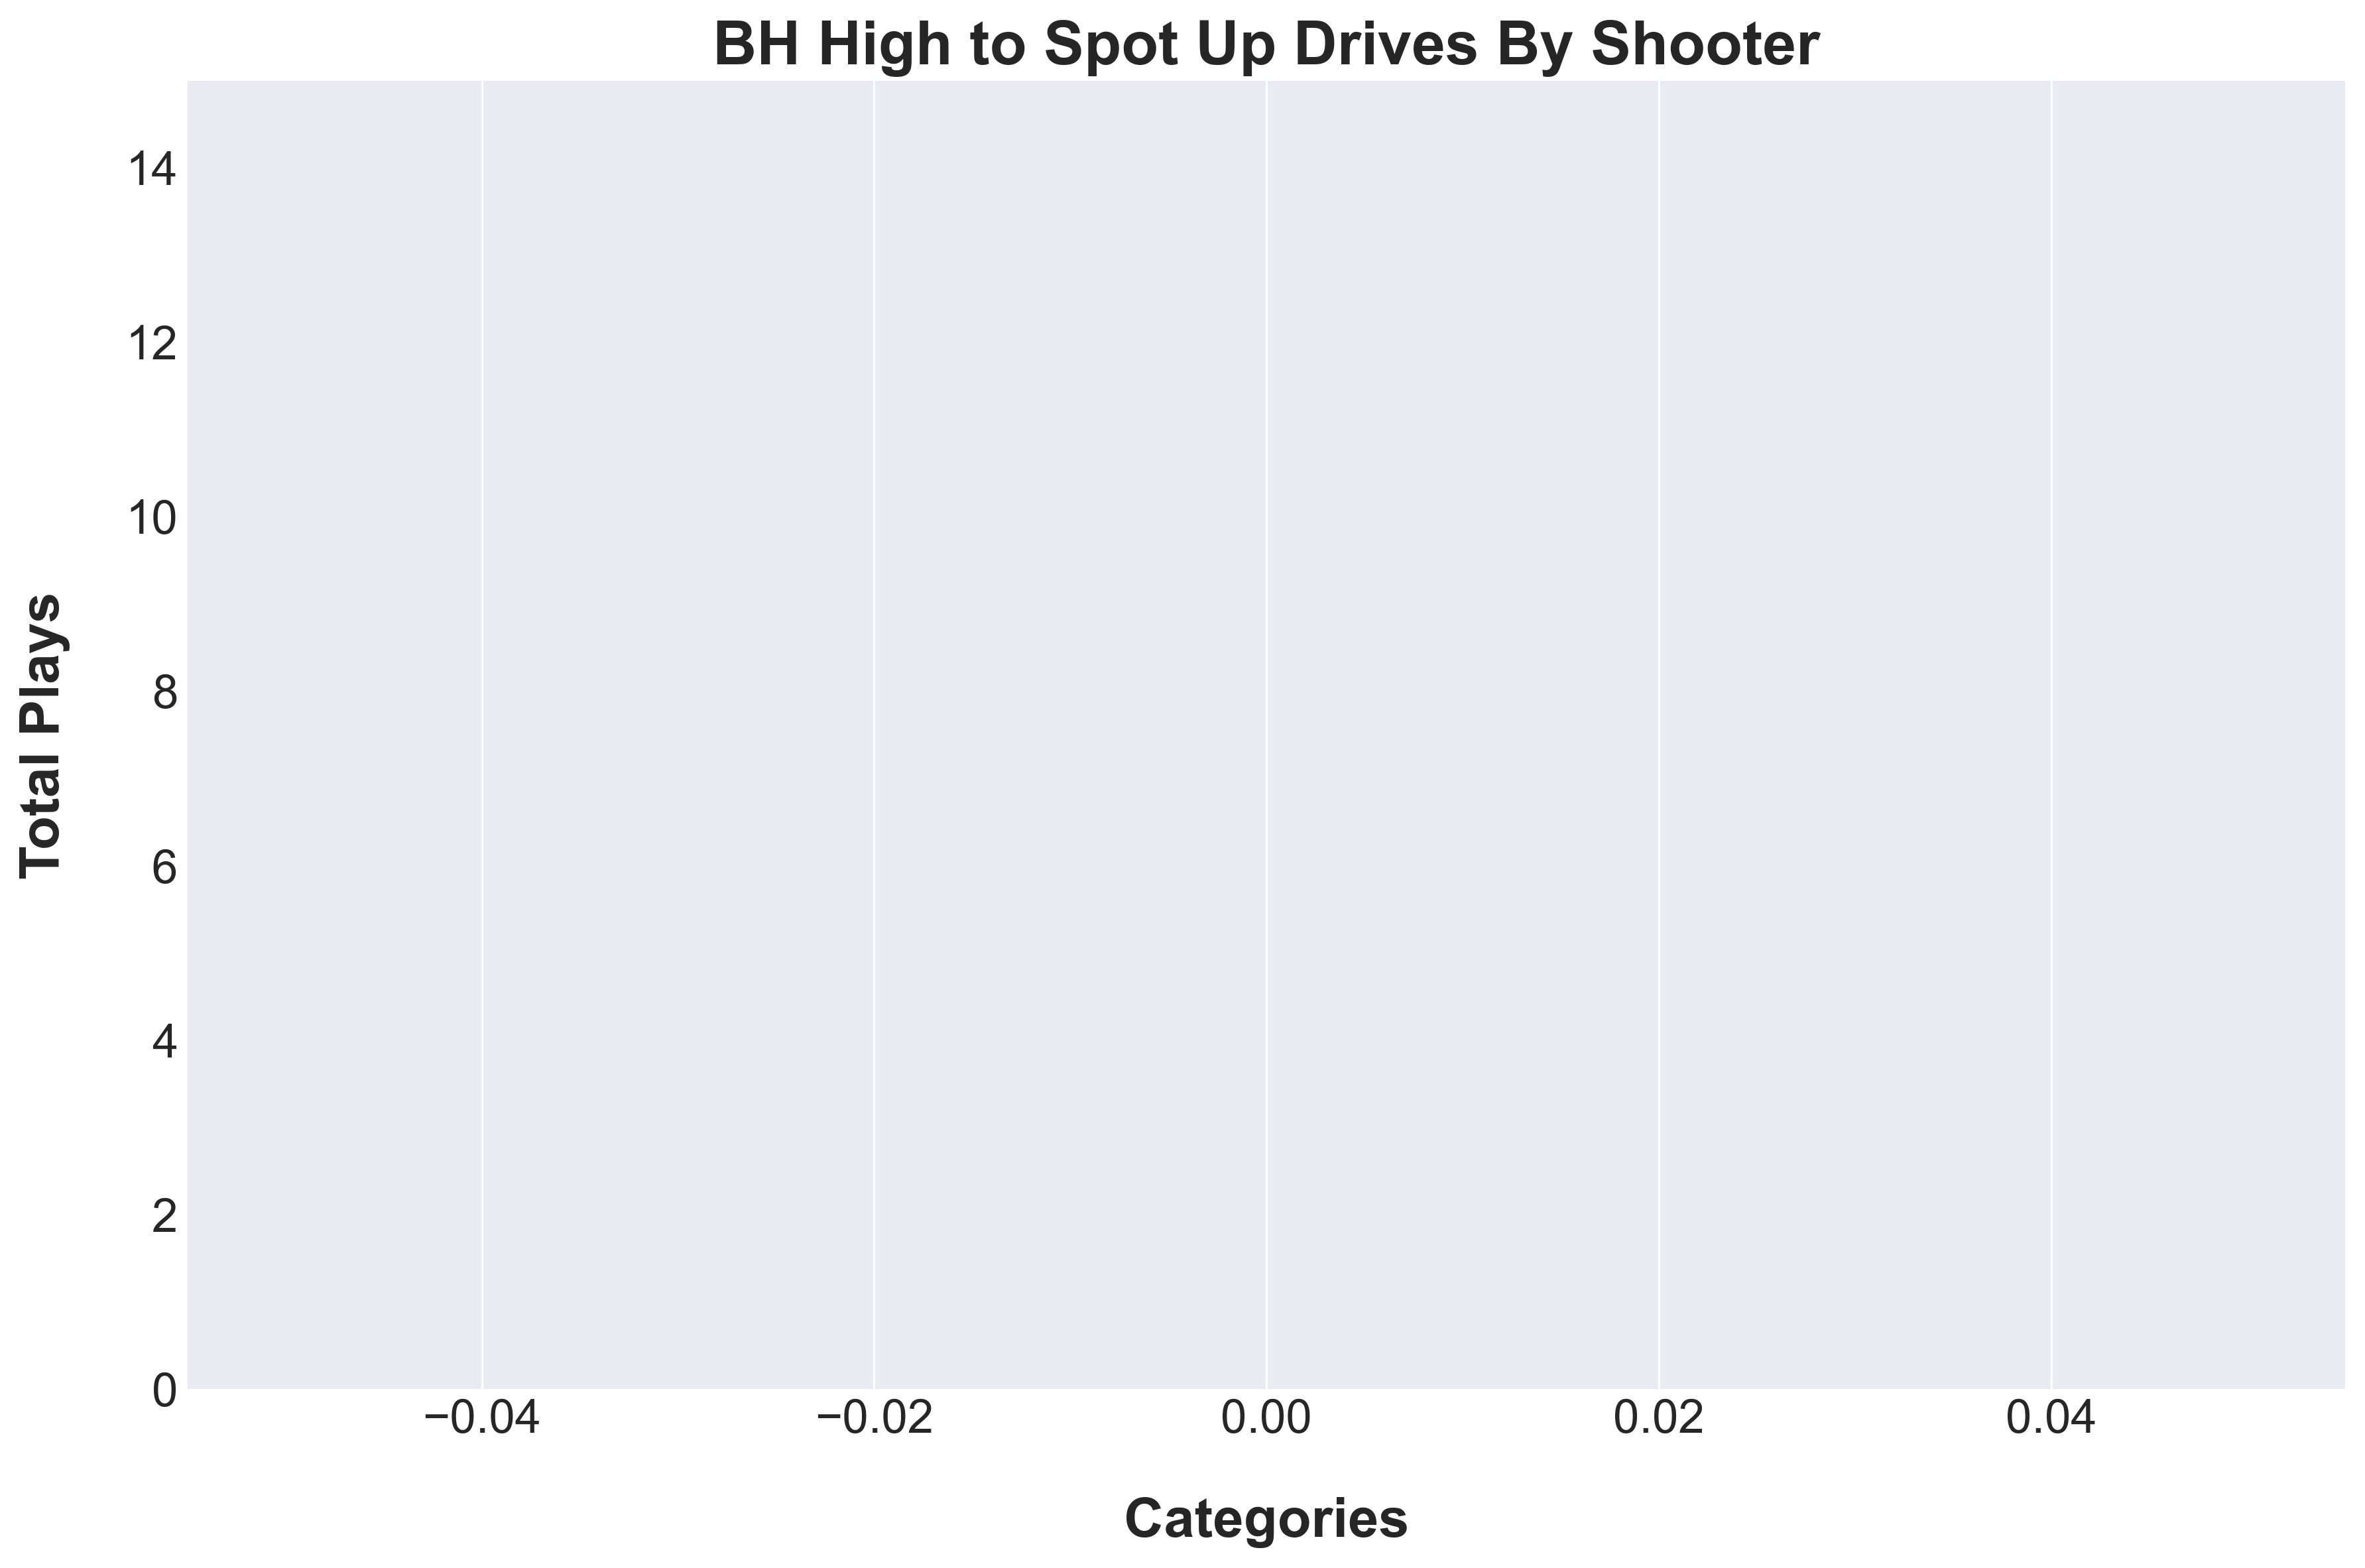
\includegraphics[width=\textwidth, height=.14\textheight]{images/PNR_PassHighDrivesPlayer_Freq.png} % Adjust the width of the image to fit
    \end{minipage}
\end{table}

\vspace{-1em} % Add vertical space before the line (optional)
%\hrule height 1pt width 1\textwidth % Adjust height and width
\vspace{-1em} % Add vertical space after the line (optional)

% BH High -> Spot Up Shots Secondary Player Stats
\begin{table}[H]
    \raisebox{3em}{ % Adjust this value to shift the tables vertically
    \begin{minipage}[t]{0.6\textwidth} % Left side (table) takes 85% of the width
        \flushleft
        \centering % Centering the title and the table
        \text{BH High - Spot Up Shots Player Statistics} % Title above the table in bold
        \vskip .25em % Adds vertical space between title and table
        \scalebox{.6}{ % Scale the entire table down by half
            \renewcommand{\arraystretch}{1.4} % Adjust the number to increase or decrease row spacing
            \begin{tabular}{
            >{\centering\arraybackslash}p{3cm} 
            >{\centering\arraybackslash}p{.75cm} 
            >{\centering\arraybackslash}p{.75cm} 
            >{\centering\arraybackslash}p{.75cm} 
            >{\centering\arraybackslash}p{.75cm} 
            >{\centering\arraybackslash}p{.75cm}
            >{\centering\arraybackslash}p{.75cm} 
            >{\centering\arraybackslash}p{.75cm}
            >{\centering\arraybackslash}p{.75cm}
            >{\centering\arraybackslash}p{.75cm} 
            >{\centering\arraybackslash}p{.75cm}}% Adjust column widths
            \toprule
            {\scriptsize \textbf{Player}} &
            {\scriptsize \textbf{Plays}} &
            {\scriptsize \textbf{3PA}} &
            {\scriptsize \textbf{3PM}} &
            {\scriptsize \textbf{3P\%}} & 
            {\scriptsize \textbf{MiA}} & 
            {\scriptsize \textbf{MiM}} &
            {\scriptsize \textbf{Mi\%}} &
            {\scriptsize \textbf{EFG\%}} &
            {\scriptsize \textbf{TO}} &
            {\scriptsize \textbf{Foul}} \\
            \midrule
            
                
            
                
            
                
            
                
            
                
            
                
            
                
            
                
            
                
                    
                        Brandon Weiss & 
                        2 & 
                        2 & 
                        1 & 
                        - & 
                        0 & 
                        0 & 
                        - & 
                        - & 
                        0 & 
                        0 \\
                    
                        Brock Bowen & 
                        7 & 
                        7 & 
                        4 & 
                        - & 
                        0 & 
                        0 & 
                        - & 
                        - & 
                        0 & 
                        0 \\
                    
                        Brody Brown & 
                        5 & 
                        5 & 
                        0 & 
                        - & 
                        0 & 
                        0 & 
                        - & 
                        - & 
                        0 & 
                        0 \\
                    
                        Jackson Otis & 
                        2 & 
                        2 & 
                        1 & 
                        - & 
                        0 & 
                        0 & 
                        - & 
                        - & 
                        0 & 
                        0 \\
                    
                        Keegan Ocorr & 
                        1 & 
                        1 & 
                        0 & 
                        - & 
                        0 & 
                        0 & 
                        - & 
                        - & 
                        0 & 
                        0 \\
                    
                        Kenny Wilburn & 
                        2 & 
                        1 & 
                        1 & 
                        - & 
                        1 & 
                        0 & 
                        - & 
                        - & 
                        0 & 
                        0 \\
                    
                        Mark Osime & 
                        1 & 
                        1 & 
                        0 & 
                        - & 
                        0 & 
                        0 & 
                        - & 
                        - & 
                        0 & 
                        0 \\
                    
                        Ronnie Toole & 
                        1 & 
                        1 & 
                        0 & 
                        - & 
                        0 & 
                        0 & 
                        - & 
                        - & 
                        0 & 
                        0 \\
                    
                
            
                
            
                
            
                
            
                
            
                
            
                
            
                
            
                
            
                
            
                
            
                
            
                
            
                
            
                
            
                
            
                
            
                
            
                
            
                
            
                
            
                
            
                
            
                
            
                
            
                
            
                
            
                
            
                
            
                
            

            \bottomrule
        \end{tabular}
        } % End of \scalebox
    \end{minipage}
    } % End of raisebox, closing the adjustment
    \hfill % This adds some flexible space between the table and the image
    \begin{minipage}[c]{0.35\textwidth} % Right side (image) takes 10% of the width
        \flushright
        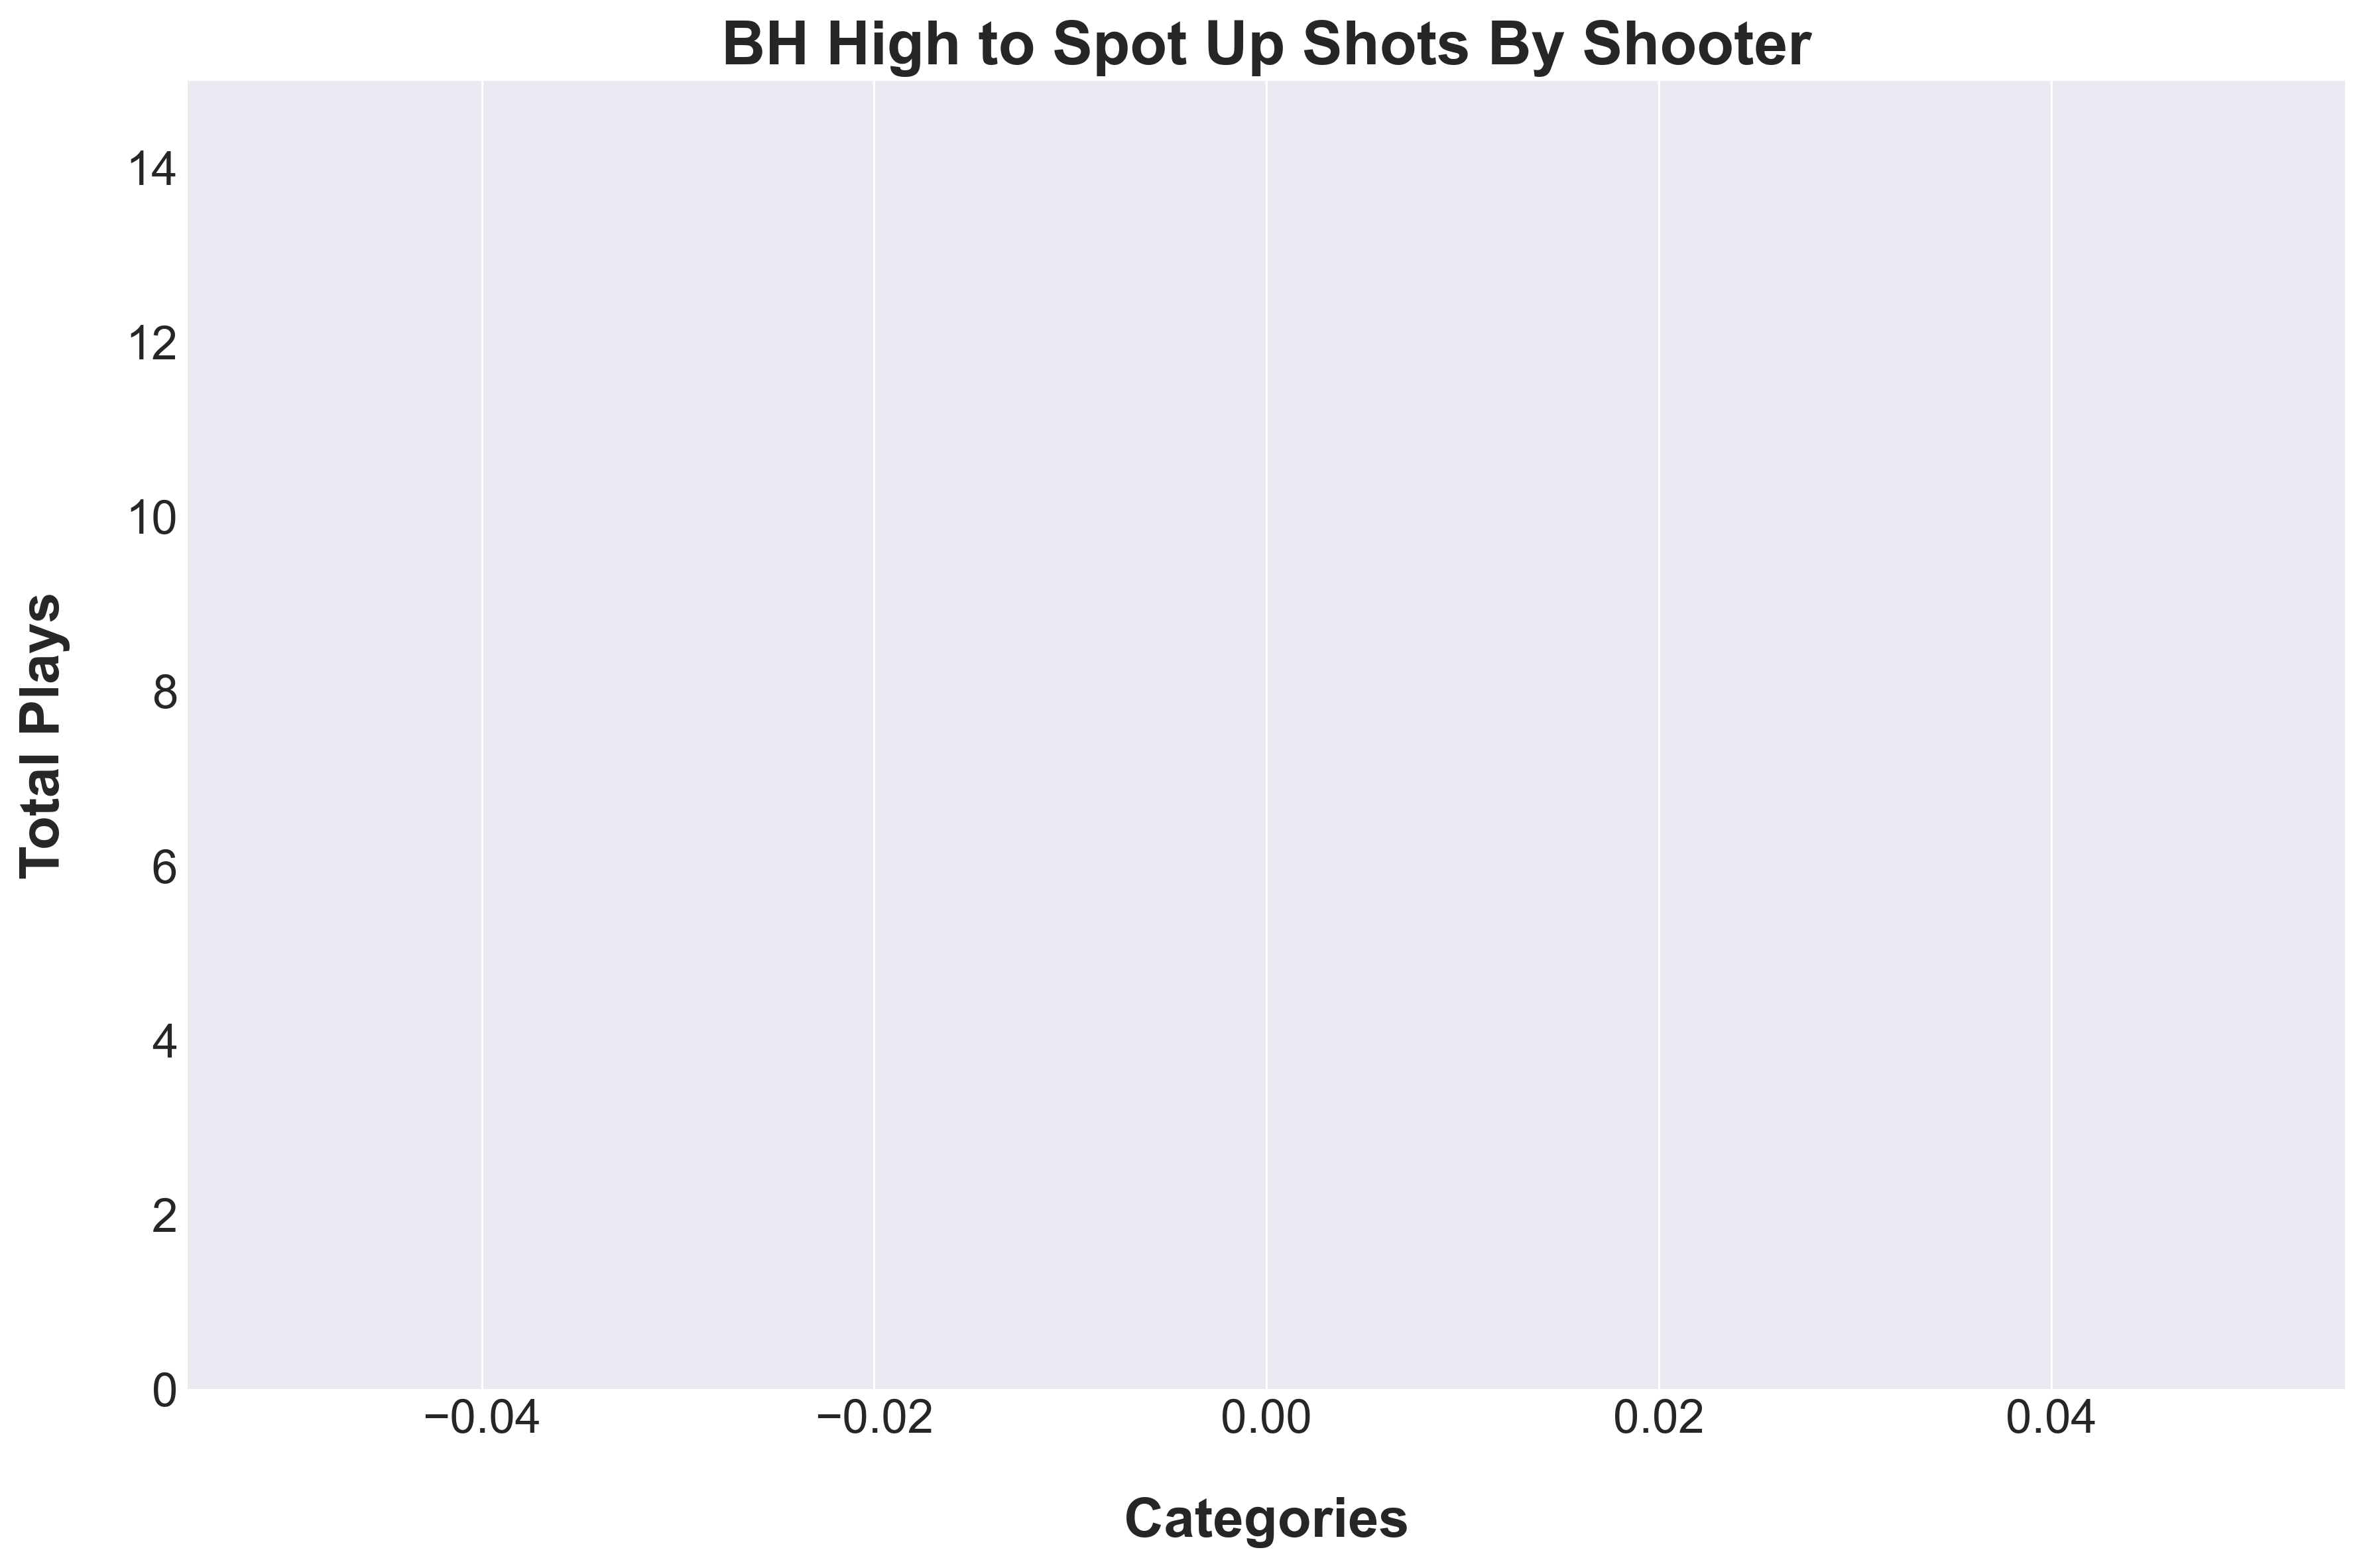
\includegraphics[width=\textwidth, height=.14\textheight]{images/PNR_PassHighShotsPlayer_Freq.png} % Adjust the width of the image to fit
    \end{minipage}
\end{table}

\vspace{-1em} % Add vertical space before the line (optional)
%\hrule height 1pt width 1\textwidth % Adjust height and width
\vspace{-1em} % Add vertical space after the line (optional)

% BH High -> Rollman Rolls Secondary Player Stats
\begin{table}[H]
    \raisebox{3em}{ % Adjust this value to shift the tables vertically
    \begin{minipage}[t]{0.6\textwidth} % Left side (table) takes 85% of the width
        \flushleft
        \centering % Centering the title and the table
        \text{BH High - Rollman Rolls Player Statistics} % Title above the table in bold
        \vskip .25em % Adds vertical space between title and table
        \scalebox{.6}{ % Scale the entire table down by half
            \renewcommand{\arraystretch}{1.4} % Adjust the number to increase or decrease row spacing
            \begin{tabular}{
            >{\centering\arraybackslash}p{3cm} 
            >{\centering\arraybackslash}p{.75cm} 
            >{\centering\arraybackslash}p{.75cm} 
            >{\centering\arraybackslash}p{.75cm} 
            >{\centering\arraybackslash}p{.75cm}
            >{\centering\arraybackslash}p{.75cm} 
            >{\centering\arraybackslash}p{.75cm}
            >{\centering\arraybackslash}p{.75cm}
            >{\centering\arraybackslash}p{.75cm} 
            >{\centering\arraybackslash}p{.75cm}}% Adjust column widths
            \toprule
            {\scriptsize \textbf{Player}} &
            {\scriptsize \textbf{Plays}} &
            {\scriptsize \textbf{2PA}} & 
            {\scriptsize \textbf{2PM}} & 
            {\scriptsize \textbf{2P\%}} & 
            {\scriptsize \textbf{MiA}} & 
            {\scriptsize \textbf{MiM}} &
            {\scriptsize \textbf{Mi\%}} &
            {\scriptsize \textbf{TO}} &
            {\scriptsize \textbf{Foul}} \\
            \midrule
            
                
            
                
            
                
            
                
            
                
            
                
            
                
            
                
            
                
            
                
                    
                        Josiah Turner & 
                        1 & 
                        1 & 
                        1 & 
                        - & 
                        0 & 
                        0 & 
                        - & 
                        0 & 
                        0 \\
                    
                        Kenny Wilburn & 
                        1 & 
                        1 & 
                        0 & 
                        - & 
                        0 & 
                        0 & 
                        - & 
                        0 & 
                        0 \\
                    
                
            
                
            
                
            
                
            
                
            
                
            
                
            
                
            
                
            
                
            
                
            
                
            
                
            
                
            
                
            
                
            
                
            
                
            
                
            
                
            
                
            
                
            
                
            
                
            
                
            
                
            
                
            
                
            
                
            

            \bottomrule
        \end{tabular}
        } % End of \scalebox
    \end{minipage}
    } % End of raisebox, closing the adjustment
    \hfill % This adds some flexible space between the table and the image
    \begin{minipage}[c]{0.35\textwidth} % Right side (image) takes 10% of the width
        \flushright
        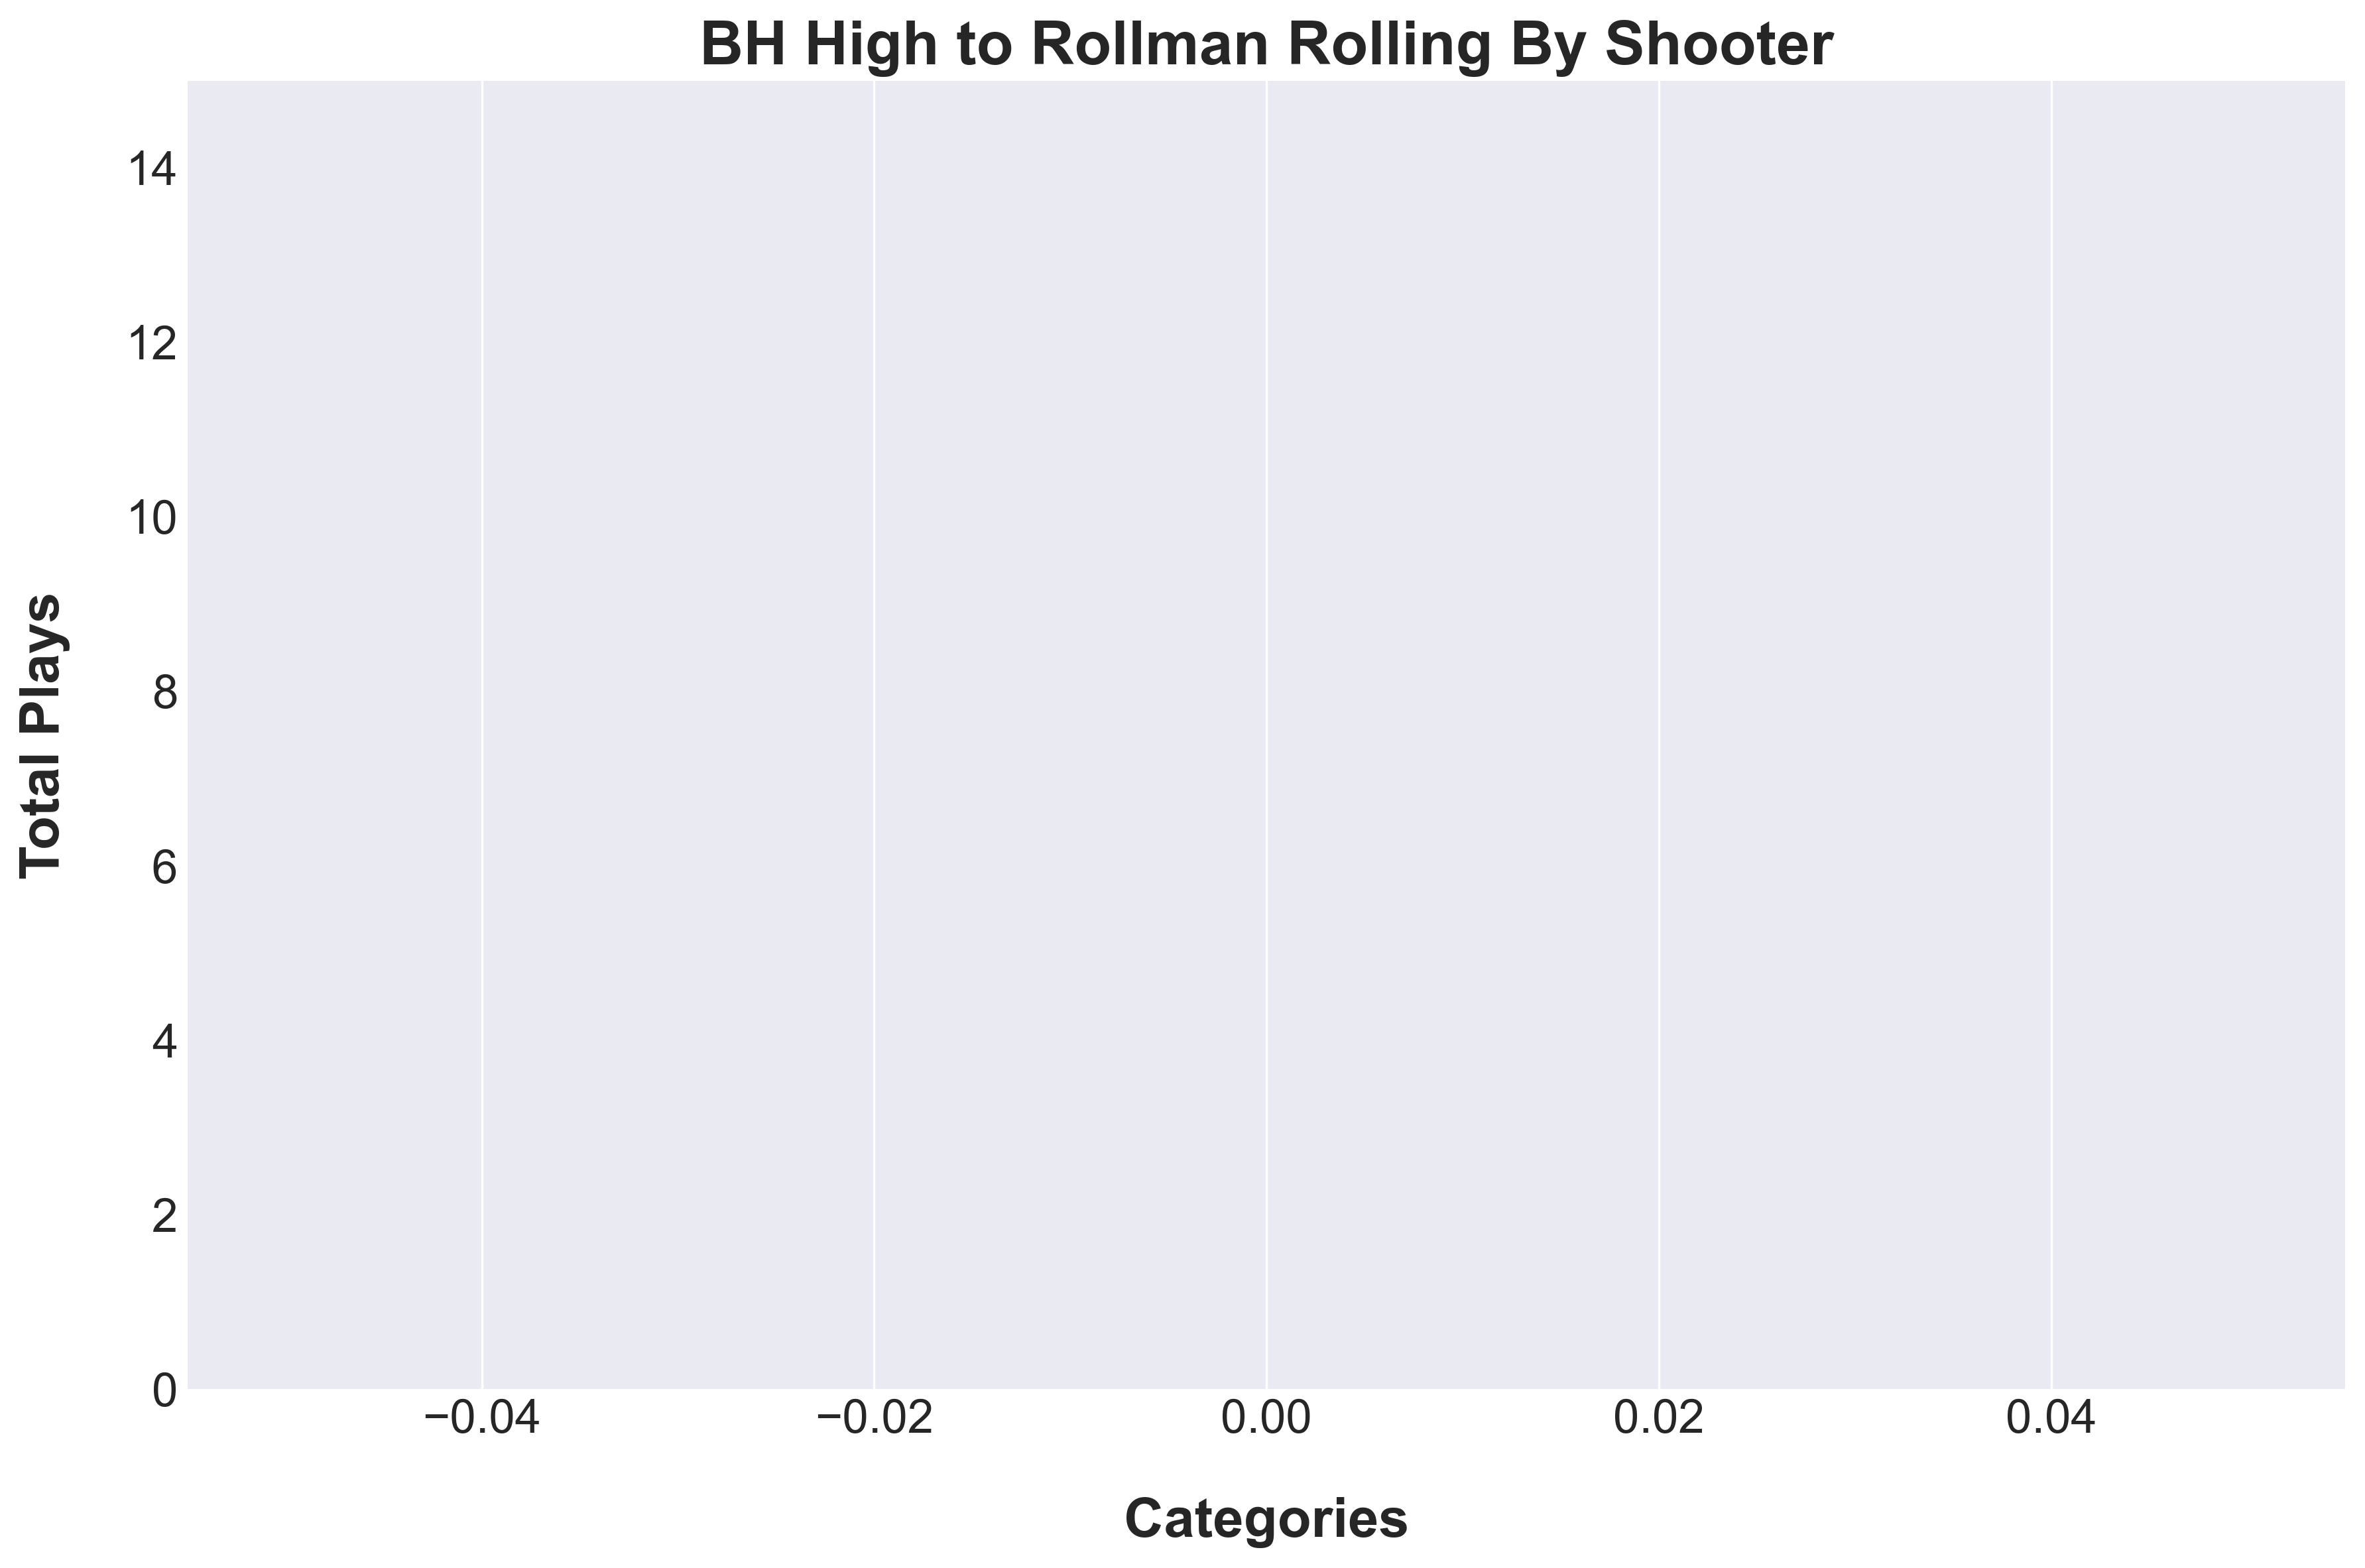
\includegraphics[width=\textwidth, height=.14\textheight]{images/PNR_PassHighRollsPlayer_Freq.png} % Adjust the width of the image to fit
    \end{minipage}
\end{table}

\vspace{-1em} % Add vertical space before the line (optional)
%\hrule height 1pt width 1\textwidth % Adjust height and width
\vspace{-1em} % Add vertical space after the line (optional)

% BH High -> Rollman Slips Secondary Player Stats
\begin{table}[H]
    \raisebox{3em}{ % Adjust this value to shift the tables vertically
    \begin{minipage}[t]{0.6\textwidth} % Left side (table) takes 85% of the width
        \flushleft
        \centering % Centering the title and the table
        \text{BH High - Rollman Slips Player Statistics} % Title above the table in bold
        \vskip .25em % Adds vertical space between title and table
        \scalebox{.55}{ % Scale the entire table down by half
            \renewcommand{\arraystretch}{1.4} % Adjust the number to increase or decrease row spacing
            \begin{tabular}{
            >{\centering\arraybackslash}p{3cm} 
            >{\centering\arraybackslash}p{.75cm} 
            >{\centering\arraybackslash}p{.75cm} 
            >{\centering\arraybackslash}p{.75cm} 
            >{\centering\arraybackslash}p{.75cm}
            >{\centering\arraybackslash}p{.75cm} 
            >{\centering\arraybackslash}p{.75cm} 
            >{\centering\arraybackslash}p{.75cm} 
            >{\centering\arraybackslash}p{.75cm}
            >{\centering\arraybackslash}p{.75cm} 
            >{\centering\arraybackslash}p{.75cm}
            >{\centering\arraybackslash}p{.75cm}
            >{\centering\arraybackslash}p{.75cm} 
            >{\centering\arraybackslash}p{.75cm}}% Adjust column widths
            \toprule
            {\scriptsize \textbf{Player}} &
            {\scriptsize \textbf{Plays}} &
            {\scriptsize \textbf{3PA}} &
            {\scriptsize \textbf{3PM}} &
            {\scriptsize \textbf{3P\%}} & 
            {\scriptsize \textbf{2PA}} & 
            {\scriptsize \textbf{2PM}} & 
            {\scriptsize \textbf{2P\%}} & 
            {\scriptsize \textbf{MiA}} & 
            {\scriptsize \textbf{MiM}} &
            {\scriptsize \textbf{Mi\%}} &
            {\scriptsize \textbf{EFG\%}} &
            {\scriptsize \textbf{TO}} &
            {\scriptsize \textbf{Foul}} \\
            \midrule
            
                
            
                
            
                
            
                
            
                
            
                
            
                
            
                
            
                
            
                
            
                
                    
                        Kenny Wilburn & 
                        1 & 
                        1 & 
                        0 & 
                        - & 
                        0 & 
                        0 & 
                        - & 
                        0 & 
                        0 & 
                        - & 
                        - & 
                        0 & 
                        0 \\
                    
                
            
                
            
                
            
                
            
                
            
                
            
                
            
                
            
                
            
                
            
                
            
                
            
                
            
                
            
                
            
                
            
                
            
                
            
                
            
                
            
                
            
                
            
                
            
                
            
                
            
                
            
                
            
                
            

            \bottomrule
        \end{tabular}
        } % End of \scalebox
    \end{minipage}
    } % End of raisebox, closing the adjustment
    \hfill % This adds some flexible space between the table and the image
    \begin{minipage}[c]{0.35\textwidth} % Right side (image) takes 10% of the width
        \flushright
        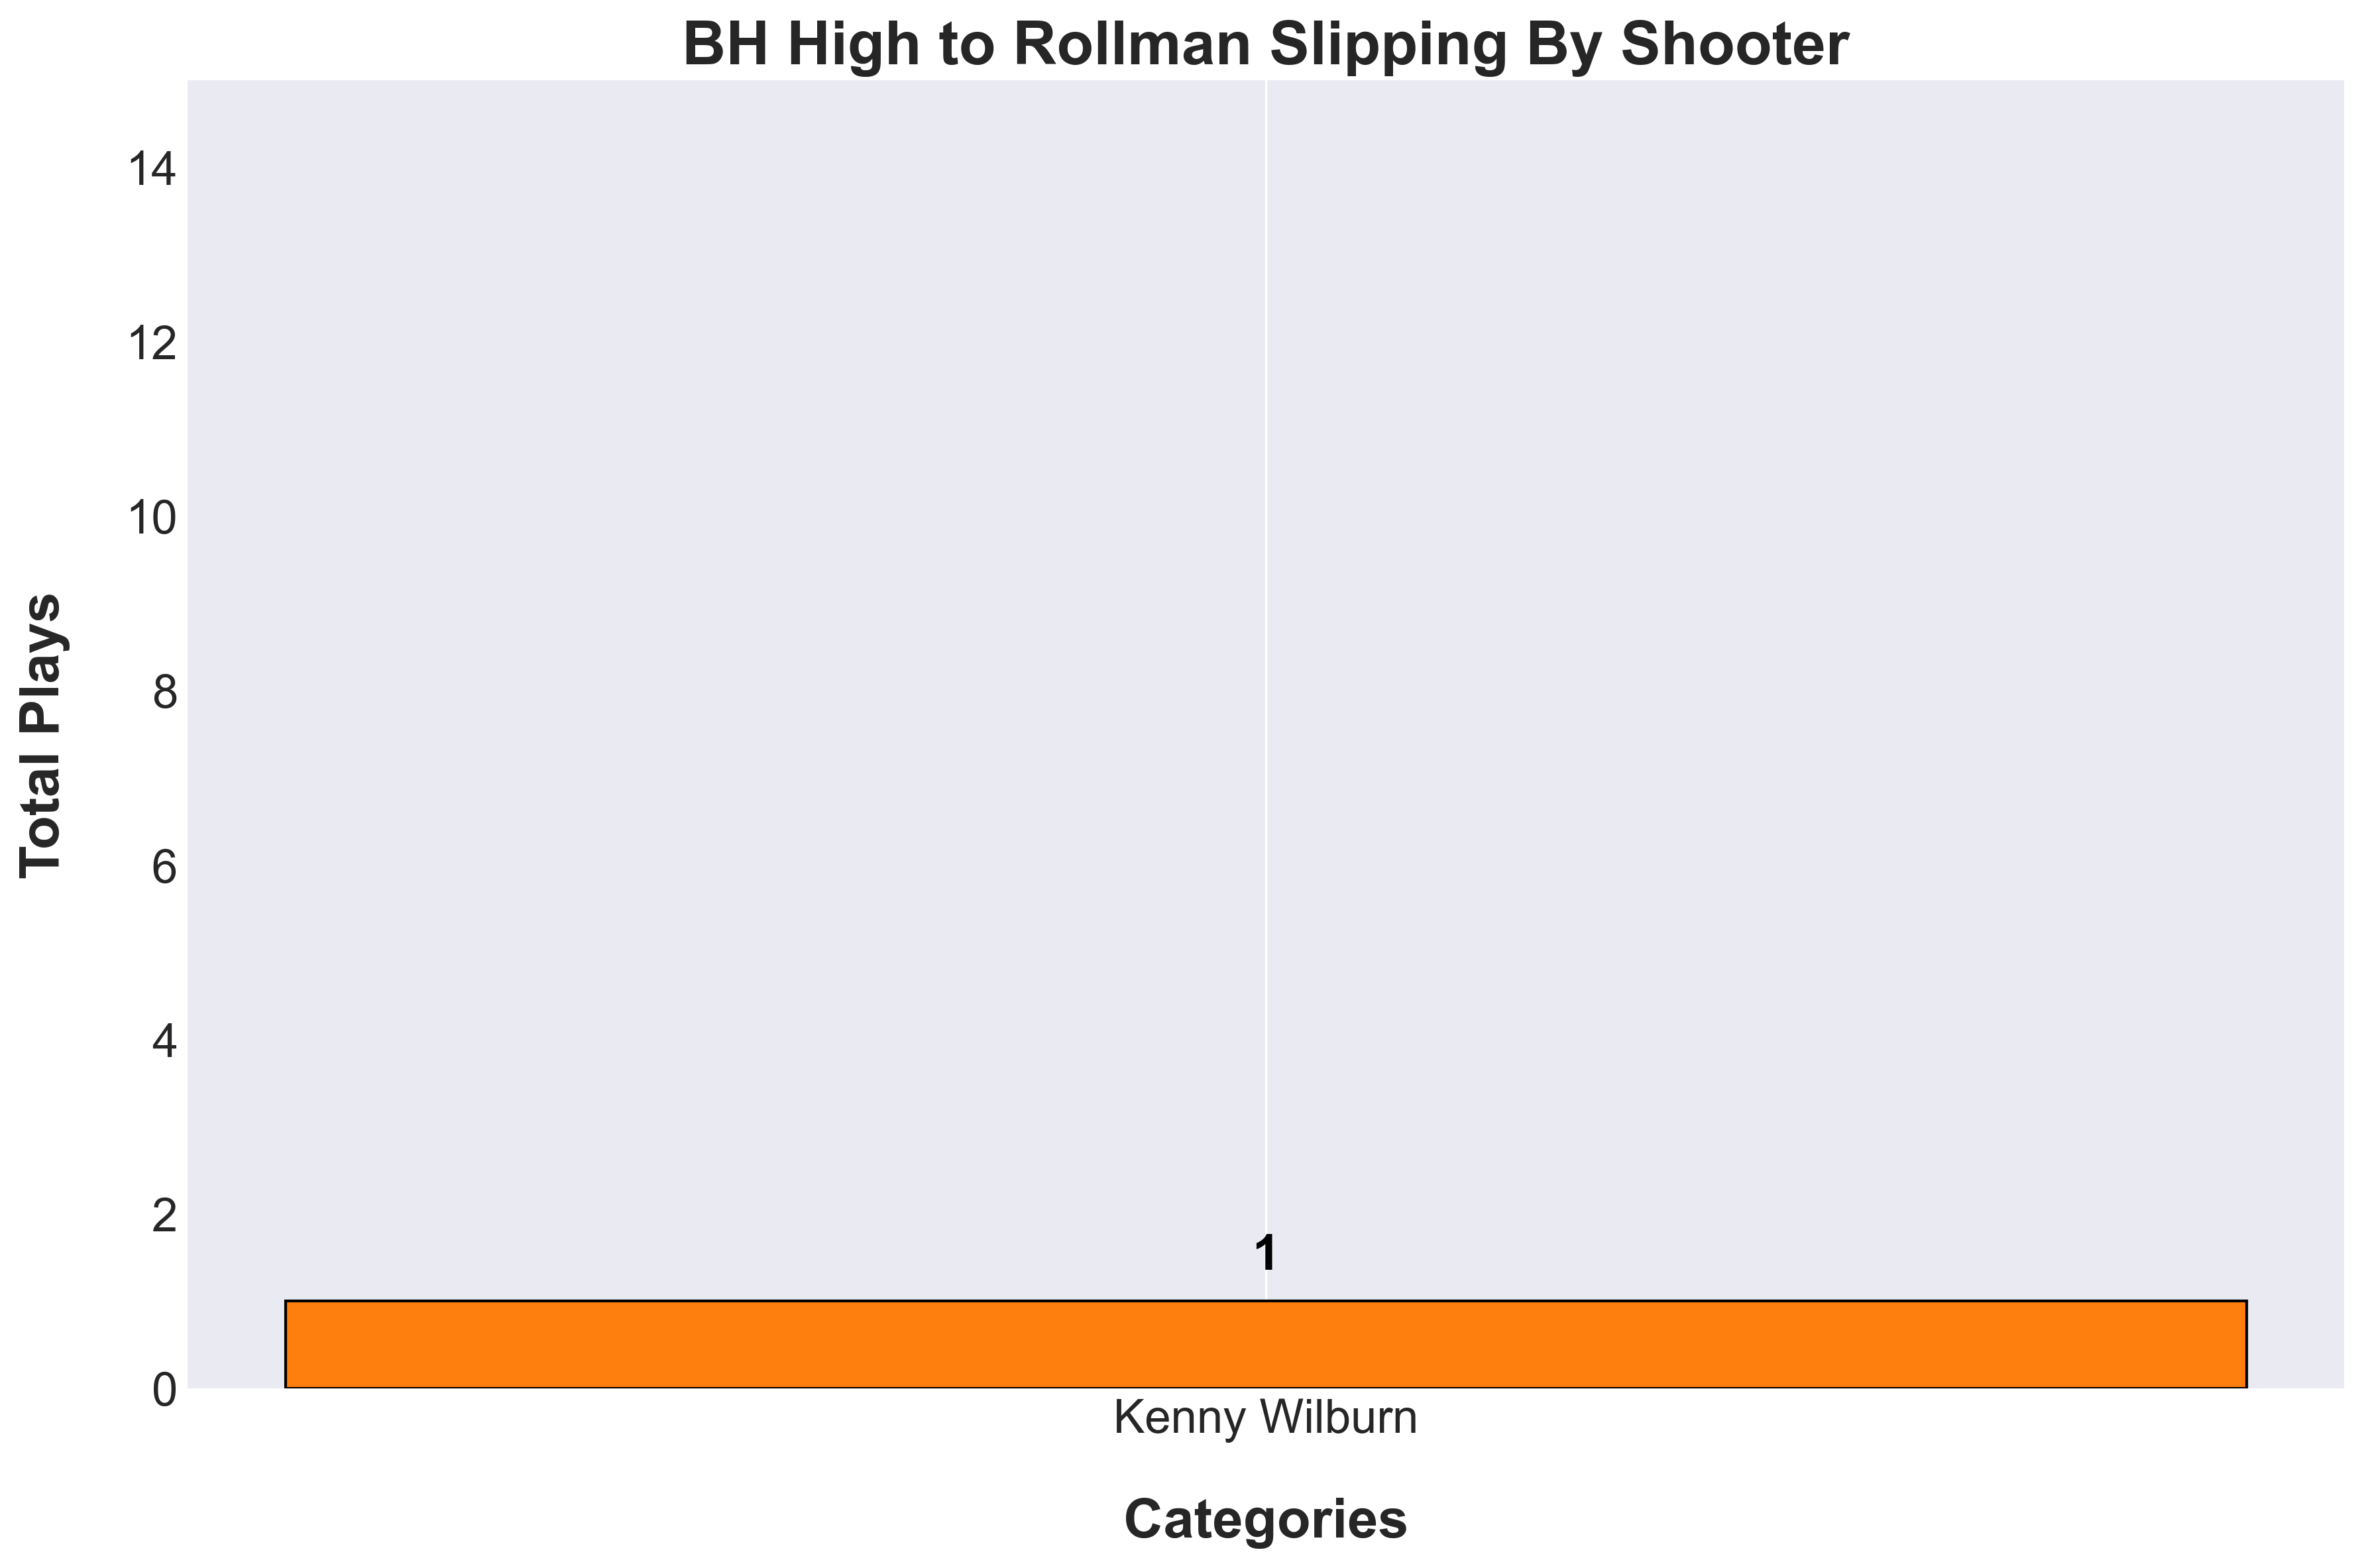
\includegraphics[width=\textwidth, height=.14\textheight]{images/PNR_PassHighSlipsPlayer_Freq.png} % Adjust the width of the image to fit
    \end{minipage}
\end{table}

\vspace{-1em} % Add vertical space before the line (optional)
%\hrule height 1pt width 1\textwidth % Adjust height and width
\vspace{-1em} % Add vertical space after the line (optional)

% BH High -> Rollman Pops Secondary Player Stats
\begin{table}[H]
    \raisebox{3em}{ % Adjust this value to shift the tables vertically
    \begin{minipage}[t]{0.6\textwidth} % Left side (table) takes 85% of the width
        \flushleft
        \centering % Centering the title and the table
        \text{BH High - Rollman Pops Player Statistics} % Title above the table in bold
        \vskip .25em % Adds vertical space between title and table
        \scalebox{.55}{ % Scale the entire table down by half
            \renewcommand{\arraystretch}{1.4} % Adjust the number to increase or decrease row spacing
            \begin{tabular}{
            >{\centering\arraybackslash}p{3cm} 
            >{\centering\arraybackslash}p{.75cm} 
            >{\centering\arraybackslash}p{.75cm} 
            >{\centering\arraybackslash}p{.75cm} 
            >{\centering\arraybackslash}p{.75cm}
            >{\centering\arraybackslash}p{.75cm} 
            >{\centering\arraybackslash}p{.75cm} 
            >{\centering\arraybackslash}p{.75cm} 
            >{\centering\arraybackslash}p{.75cm}
            >{\centering\arraybackslash}p{.75cm} 
            >{\centering\arraybackslash}p{.75cm}
            >{\centering\arraybackslash}p{.75cm}
            >{\centering\arraybackslash}p{.75cm} 
            >{\centering\arraybackslash}p{.75cm}}% Adjust column widths
            \toprule
            {\scriptsize \textbf{Player}} &
            {\scriptsize \textbf{Plays}} &
            {\scriptsize \textbf{3PA}} &
            {\scriptsize \textbf{3PM}} &
            {\scriptsize \textbf{3P\%}} & 
            {\scriptsize \textbf{2PA}} & 
            {\scriptsize \textbf{2PM}} & 
            {\scriptsize \textbf{2P\%}} & 
            {\scriptsize \textbf{MiA}} & 
            {\scriptsize \textbf{MiM}} &
            {\scriptsize \textbf{Mi\%}} &
            {\scriptsize \textbf{EFG\%}} &
            {\scriptsize \textbf{TO}} &
            {\scriptsize \textbf{Foul}} \\
            \midrule
            
                
            
                
            
                
            
                
            
                
            
                
            
                
            
                
            
                
            
                
            
                
            
                
                    
                        Josiah Turner & 
                        6 & 
                        3 & 
                        0 & 
                        - & 
                        2 & 
                        0 & 
                        - & 
                        0 & 
                        0 & 
                        - & 
                        - & 
                        0 & 
                        1 \\
                    
                        Kenny Wilburn & 
                        2 & 
                        2 & 
                        1 & 
                        - & 
                        0 & 
                        0 & 
                        - & 
                        0 & 
                        0 & 
                        - & 
                        - & 
                        0 & 
                        0 \\
                    
                
            
                
            
                
            
                
            
                
            
                
            
                
            
                
            
                
            
                
            
                
            
                
            
                
            
                
            
                
            
                
            
                
            
                
            
                
            
                
            
                
            
                
            
                
            
                
            
                
            
                
            
                
            

            \bottomrule
        \end{tabular}
        } % End of \scalebox
    \end{minipage}
    } % End of raisebox, closing the adjustment
    \hfill % This adds some flexible space between the table and the image
    \begin{minipage}[c]{0.35\textwidth} % Right side (image) takes 10% of the width
        \flushright
        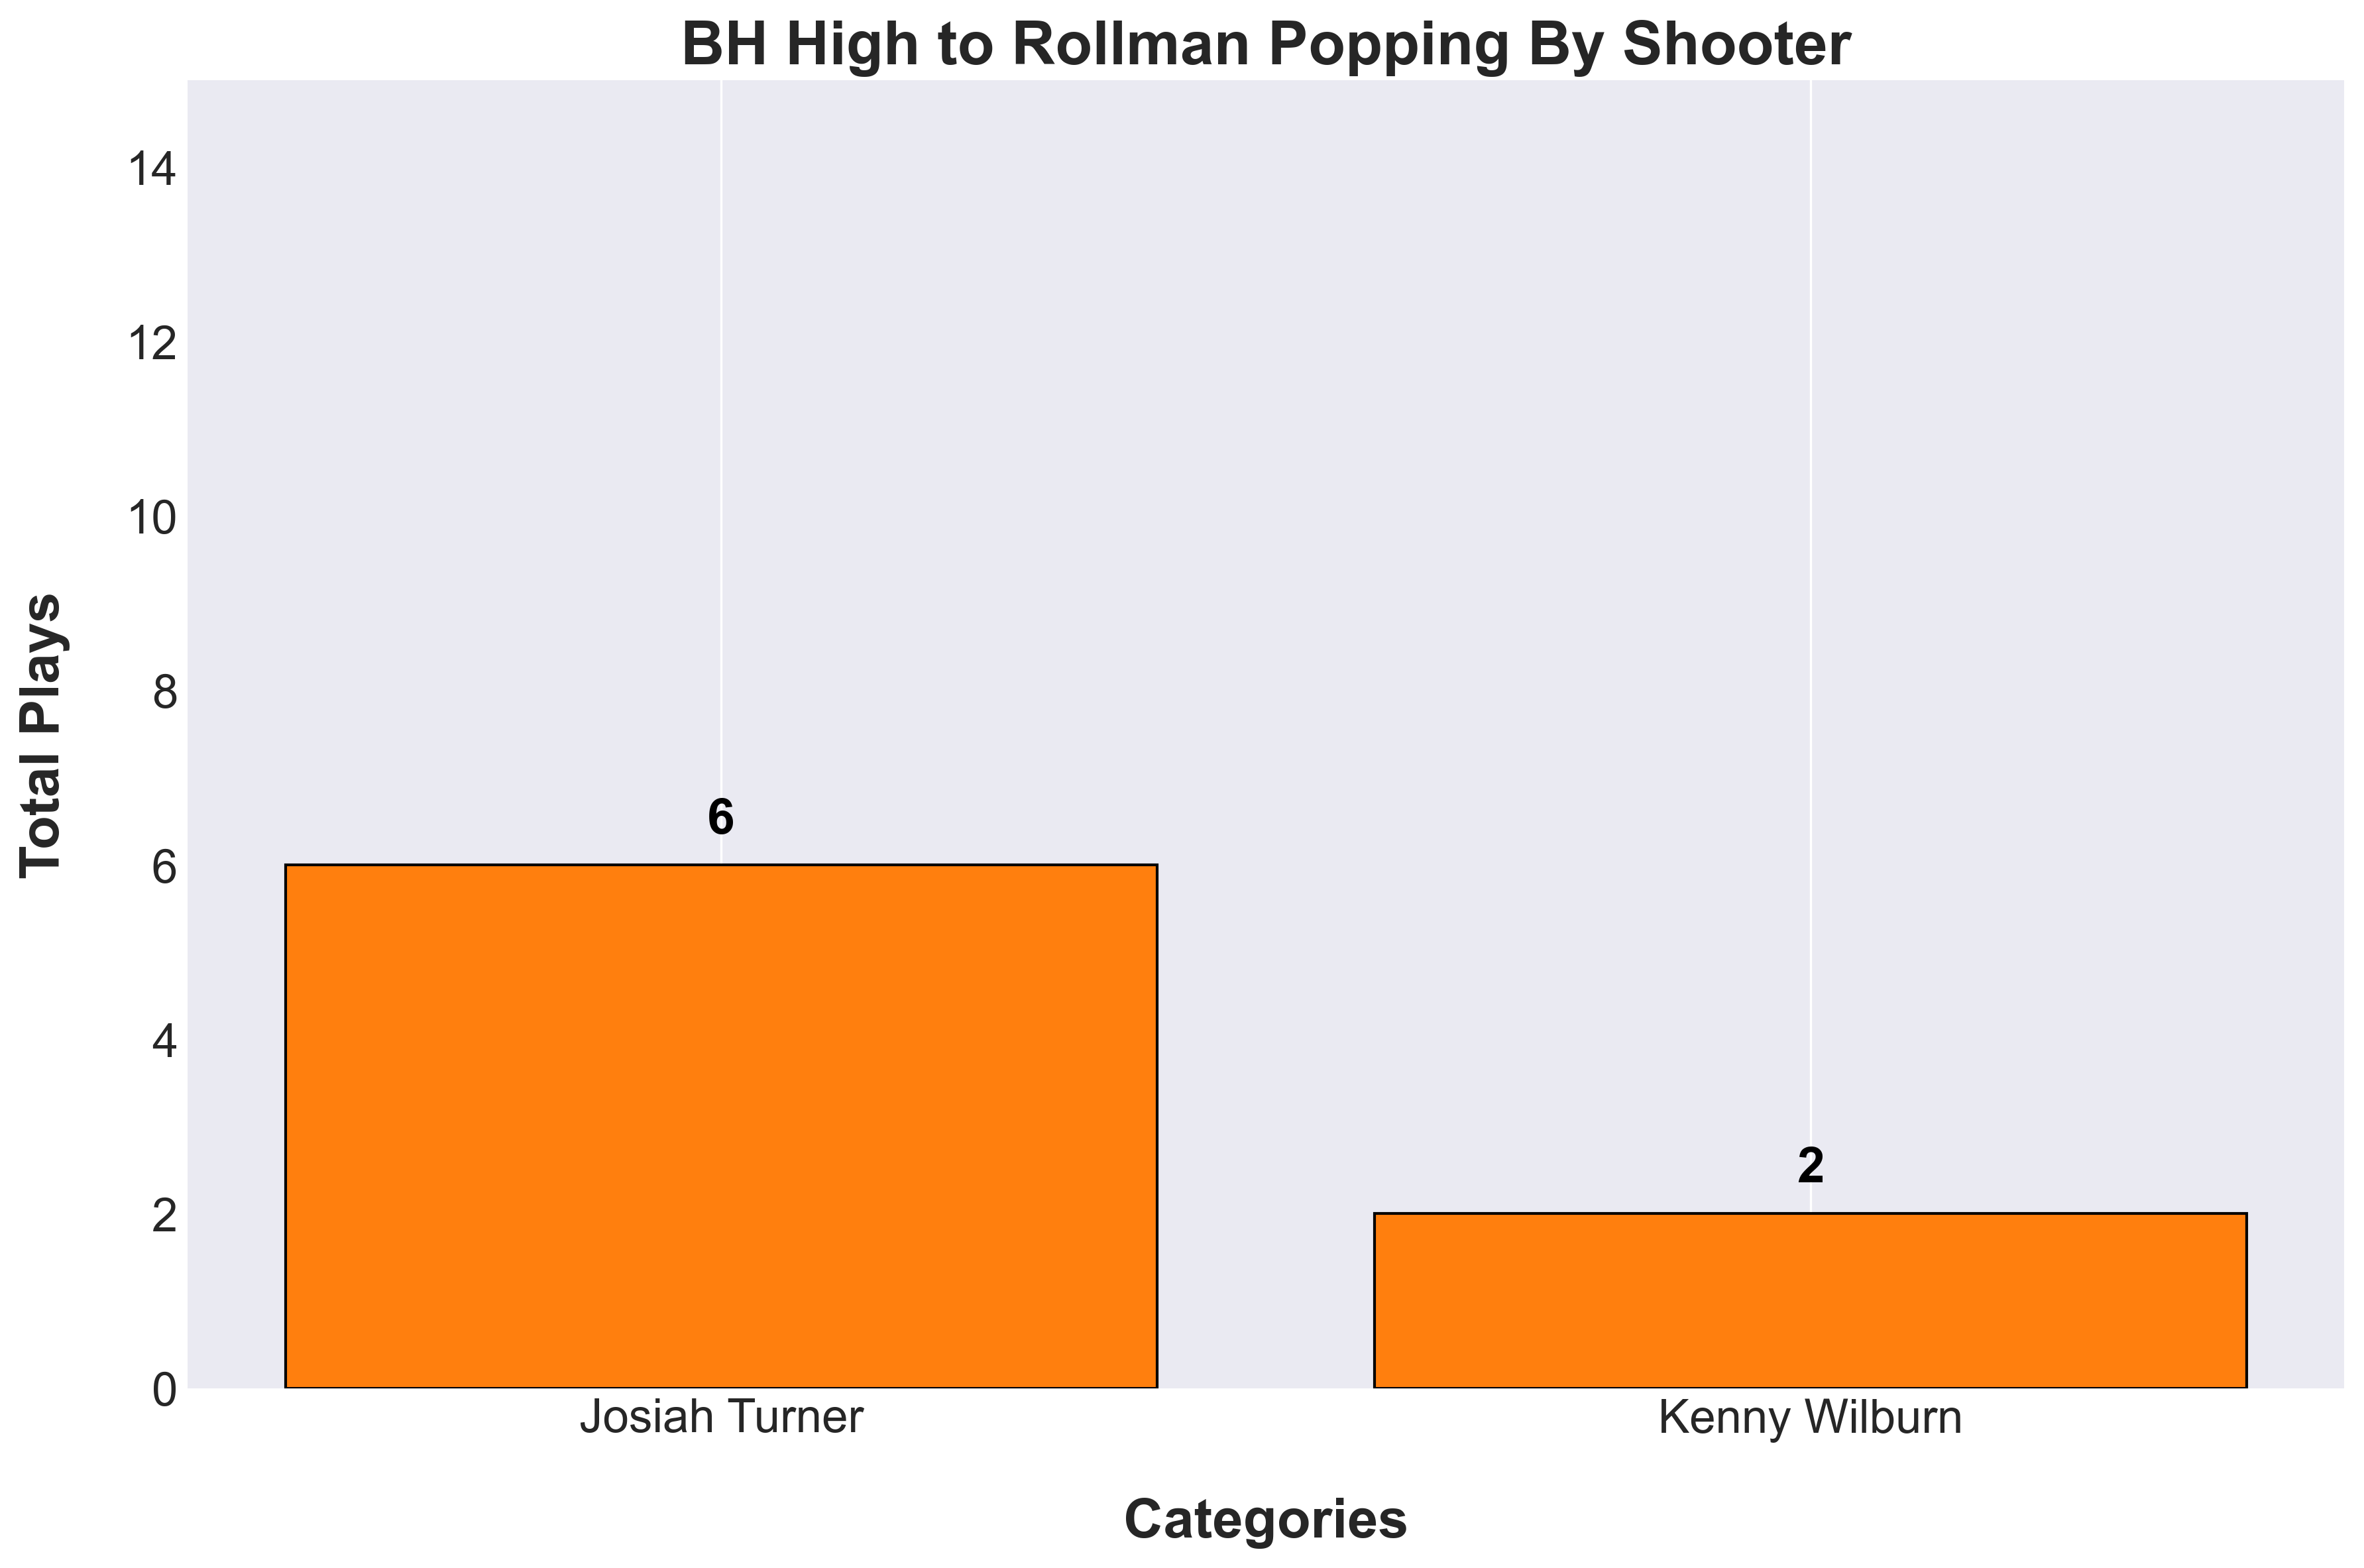
\includegraphics[width=\textwidth, height=.14\textheight]{images/PNR_PassHighPopsPlayer_Freq.png} % Adjust the width of the image to fit
    \end{minipage}
\end{table}

\vspace{-1em} % Add vertical space before the line (optional)
\hrule height 1pt width 1\textwidth % Adjust height and width
\vspace{1 em} % Add vertical space after the line (optional)

\subsubsection{BH Left PNR Passer Statistics}

% BH Left -> Cuts Secondary Player Stats
\begin{table}[H]
    \raisebox{3em}{ % Adjust this value to shift the tables vertically
    \begin{minipage}[t]{0.6\textwidth} % Left side (table) takes 85% of the width
        \flushleft
        \centering % Centering the title and the table
        \text{BH Left - Cuts Player Statistics} % Title above the table in bold
        \vskip .25em % Adds vertical space between title and table
        \scalebox{.6}{ % Scale the entire table down by half
            \renewcommand{\arraystretch}{1.4} % Adjust the number to increase or decrease row spacing
            \begin{tabular}{
            >{\centering\arraybackslash}p{3cm} 
            >{\centering\arraybackslash}p{.75cm} 
            >{\centering\arraybackslash}p{.75cm} 
            >{\centering\arraybackslash}p{.75cm} 
            >{\centering\arraybackslash}p{.75cm}
            >{\centering\arraybackslash}p{.75cm} 
            >{\centering\arraybackslash}p{.75cm}
            >{\centering\arraybackslash}p{.75cm}
            >{\centering\arraybackslash}p{.75cm} 
            >{\centering\arraybackslash}p{.75cm}}% Adjust column widths
            \toprule
            {\scriptsize \textbf{Player}} &
            {\scriptsize \textbf{Plays}} &
            {\scriptsize \textbf{2PA}} & 
            {\scriptsize \textbf{2PM}} & 
            {\scriptsize \textbf{2P\%}} & 
            {\scriptsize \textbf{MiA}} & 
            {\scriptsize \textbf{MiM}} &
            {\scriptsize \textbf{Mi\%}} &
            {\scriptsize \textbf{TO}} &
            {\scriptsize \textbf{Foul}} \\
            \midrule
            
                
            
                
            
                
            
                
            
                
            
                
            
                
            
                
            
                
            
                
            
                
            
                
            
                
                    
                
            
                
            
                
            
                
            
                
            
                
            
                
            
                
            
                
            
                
            
                
            
                
            
                
            
                
            
                
            
                
            
                
            
                
            
                
            
                
            
                
            
                
            
                
            
                
            
                
            
                
            

            \bottomrule
        \end{tabular}
        } % End of \scalebox
    \end{minipage}
    } % End of raisebox, closing the adjustment
    \hfill % This adds some flexible space between the table and the image
    \begin{minipage}[c]{0.35\textwidth} % Right side (image) takes 10% of the width
        \flushright
        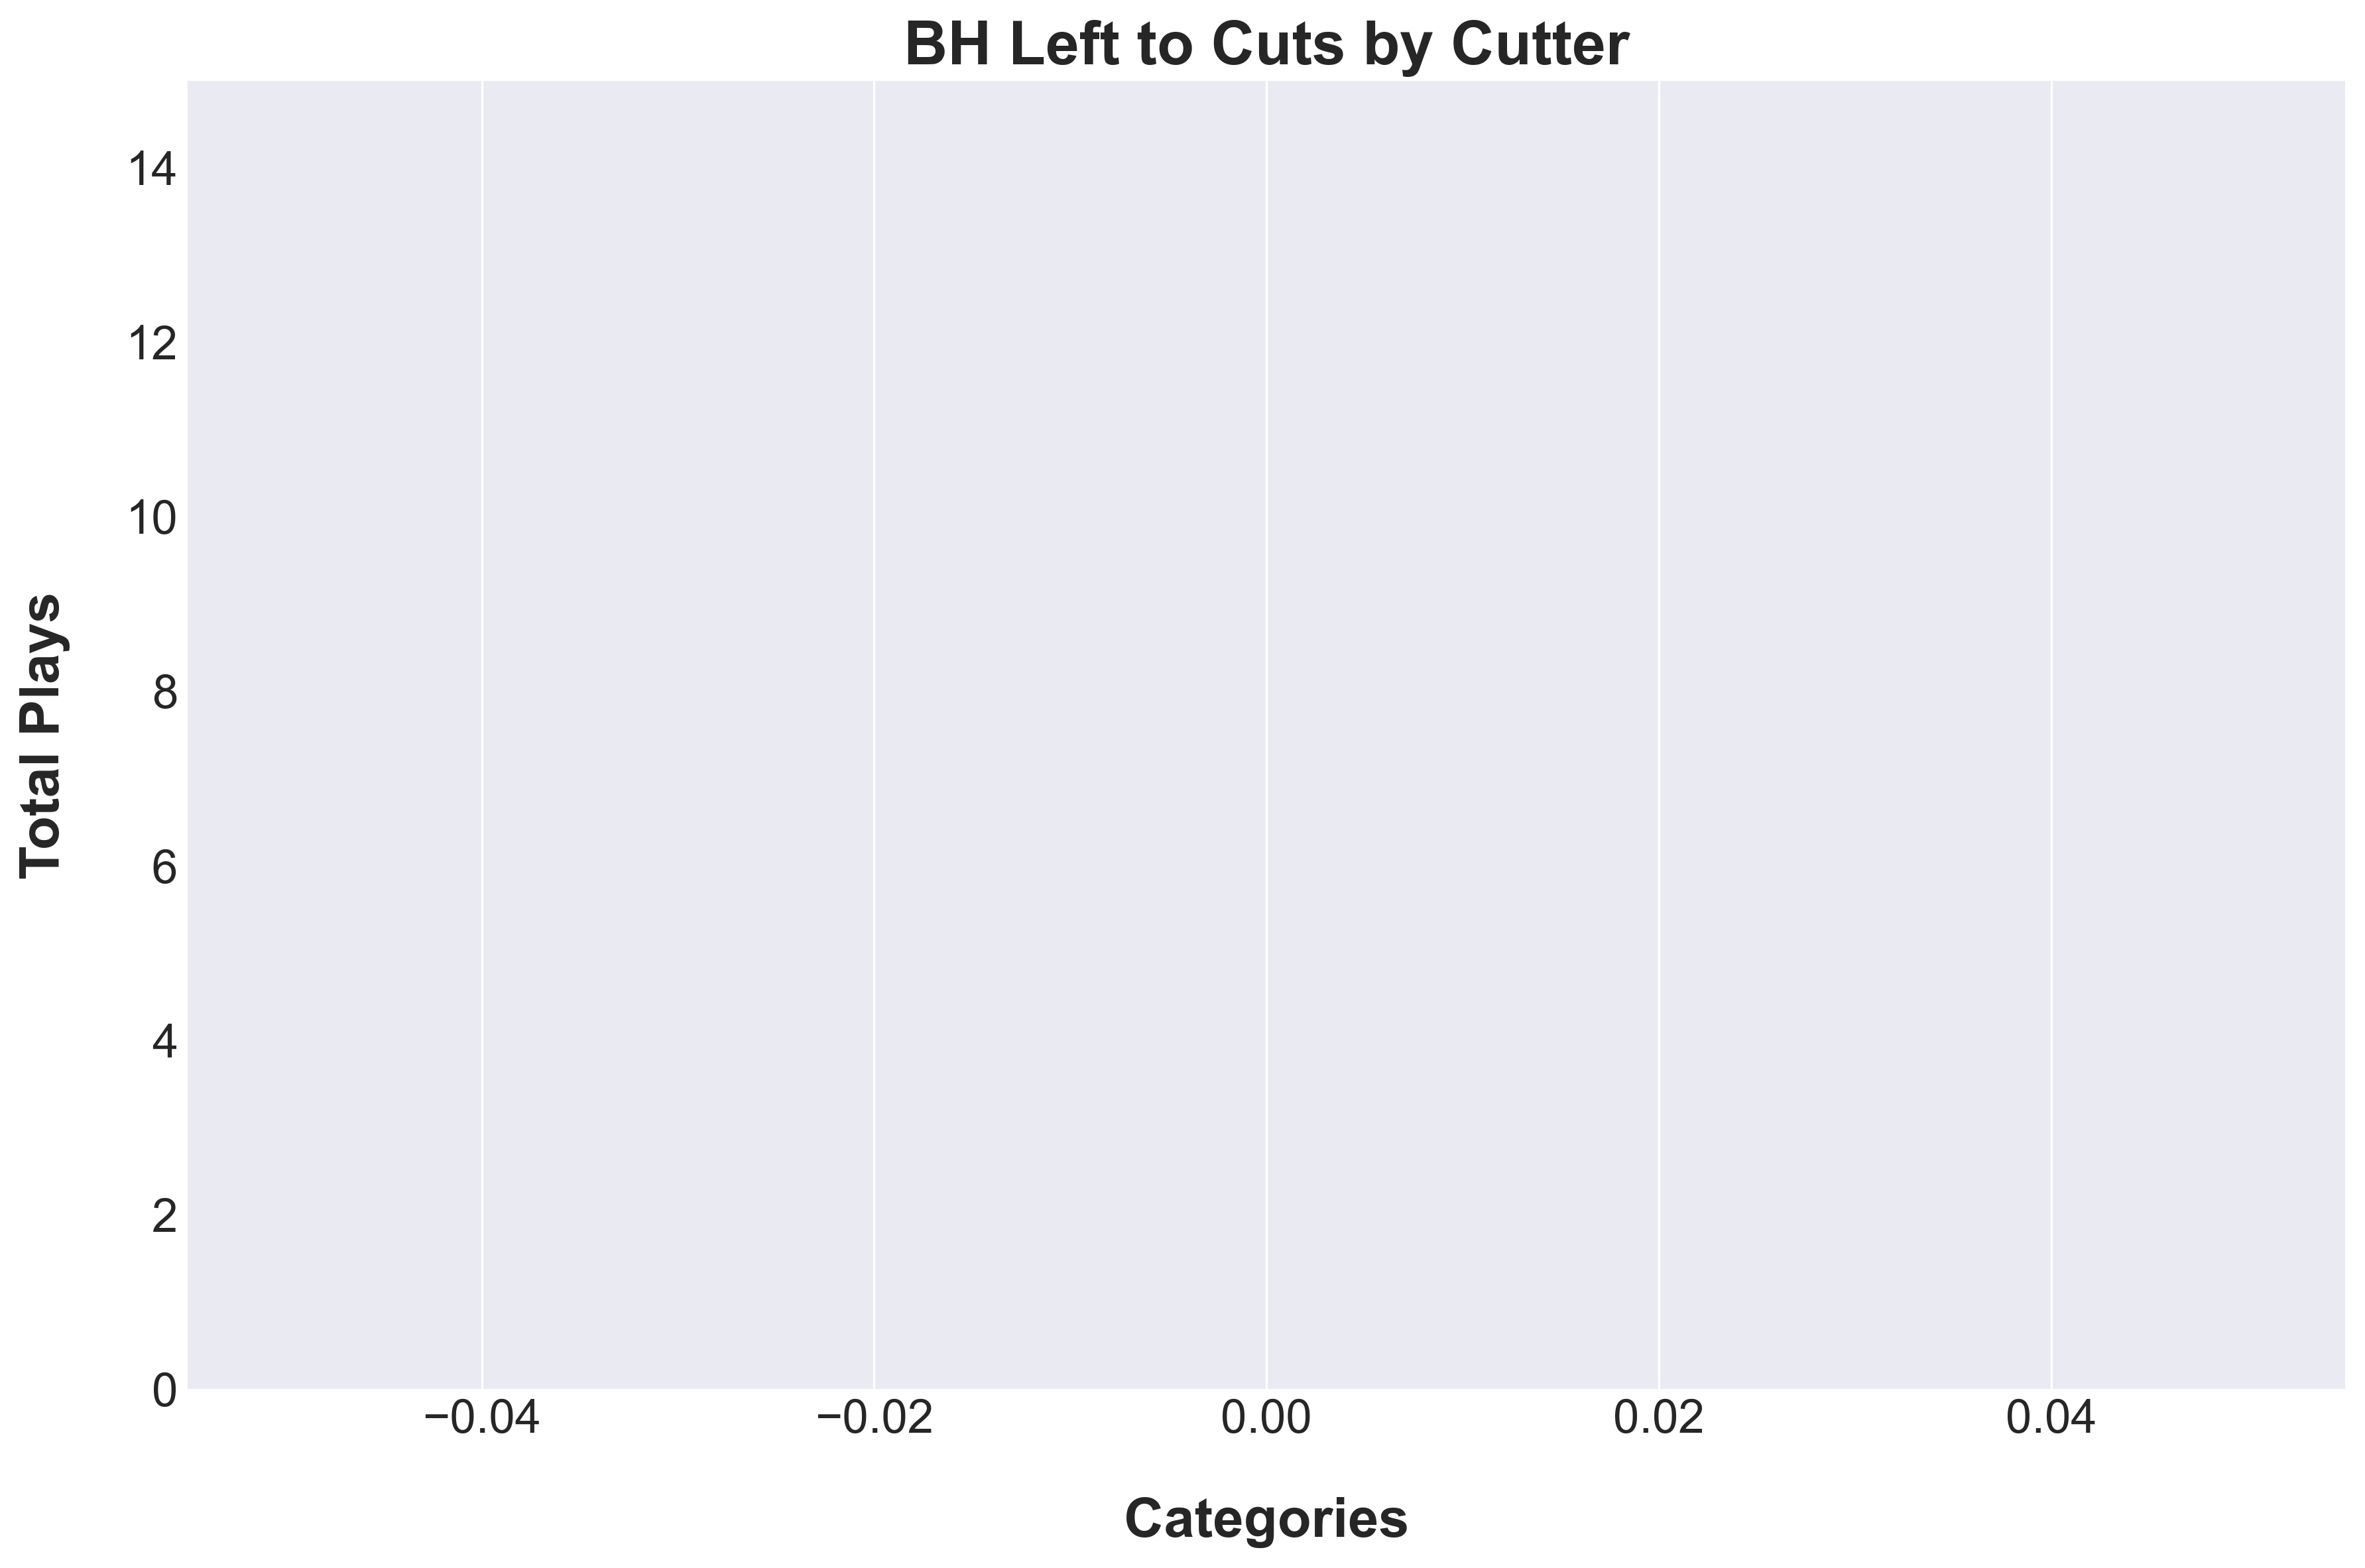
\includegraphics[width=\textwidth, height=.14\textheight]{images/PNR_PassLeftCutsPlayer_Freq.png} % Adjust the width of the image to fit
    \end{minipage}
\end{table}

\vspace{-1em} % Add vertical space before the line (optional)
%\hrule height 1pt width 1\textwidth % Adjust height and width
\vspace{-1em} % Add vertical space after the line (optional)

% BH Left -> Spot Up Drives Secondary Player Stats
\begin{table}[H]
    \raisebox{3em}{ % Adjust this value to shift the tables vertically
    \begin{minipage}[t]{0.6\textwidth} % Left side (table) takes 85% of the width
        \flushleft
        \centering % Centering the title and the table
        \text{BH Left - Spot Up Drives Player Statistics} % Title above the table in bold
        \vskip .25em % Adds vertical space between title and table
        \scalebox{.55}{ % Scale the entire table down by half
            \renewcommand{\arraystretch}{1.4} % Adjust the number to increase or decrease row spacing
            \begin{tabular}{
            >{\centering\arraybackslash}p{3cm} 
            >{\centering\arraybackslash}p{.75cm} 
            >{\centering\arraybackslash}p{.75cm} 
            >{\centering\arraybackslash}p{.75cm} 
            >{\centering\arraybackslash}p{.75cm}
            >{\centering\arraybackslash}p{.75cm} 
            >{\centering\arraybackslash}p{.75cm} 
            >{\centering\arraybackslash}p{.75cm} 
            >{\centering\arraybackslash}p{.75cm}
            >{\centering\arraybackslash}p{.75cm} 
            >{\centering\arraybackslash}p{.75cm}
            >{\centering\arraybackslash}p{.75cm}
            >{\centering\arraybackslash}p{.75cm} 
            >{\centering\arraybackslash}p{.75cm}}% Adjust column widths
            \toprule
            {\scriptsize \textbf{Player}} &
            {\scriptsize \textbf{Plays}} &
            {\scriptsize \textbf{3PA}} &
            {\scriptsize \textbf{3PM}} &
            {\scriptsize \textbf{3P\%}} & 
            {\scriptsize \textbf{2PA}} & 
            {\scriptsize \textbf{2PM}} & 
            {\scriptsize \textbf{2P\%}} & 
            {\scriptsize \textbf{MiA}} & 
            {\scriptsize \textbf{MiM}} &
            {\scriptsize \textbf{Mi\%}} &
            {\scriptsize \textbf{EFG\%}} &
            {\scriptsize \textbf{TO}} &
            {\scriptsize \textbf{Foul}} \\
            \midrule
            
                
            
                
            
                
            
                
            
                
            
                
            
                
            
                
            
                
            
                
            
                
            
                
            
                
            
                
                    
                        Ronnie Toole & 
                        1 & 
                        0 & 
                        0 & 
                        - & 
                        1 & 
                        0 & 
                        - & 
                        0 & 
                        0 & 
                        - & 
                        - & 
                        0 & 
                        0 \\
                    
                        Zac Ditzel & 
                        1 & 
                        0 & 
                        0 & 
                        - & 
                        1 & 
                        0 & 
                        - & 
                        0 & 
                        0 & 
                        - & 
                        - & 
                        0 & 
                        0 \\
                    
                
            
                
            
                
            
                
            
                
            
                
            
                
            
                
            
                
            
                
            
                
            
                
            
                
            
                
            
                
            
                
            
                
            
                
            
                
            
                
            
                
            
                
            
                
            
                
            
                
            

            \bottomrule
        \end{tabular}
        } % End of \scalebox
    \end{minipage}
    } % End of raisebox, closing the adjustment
    \hfill % This adds some flexible space between the table and the image
    \begin{minipage}[c]{0.35\textwidth} % Right side (image) takes 10% of the width
        \flushright
        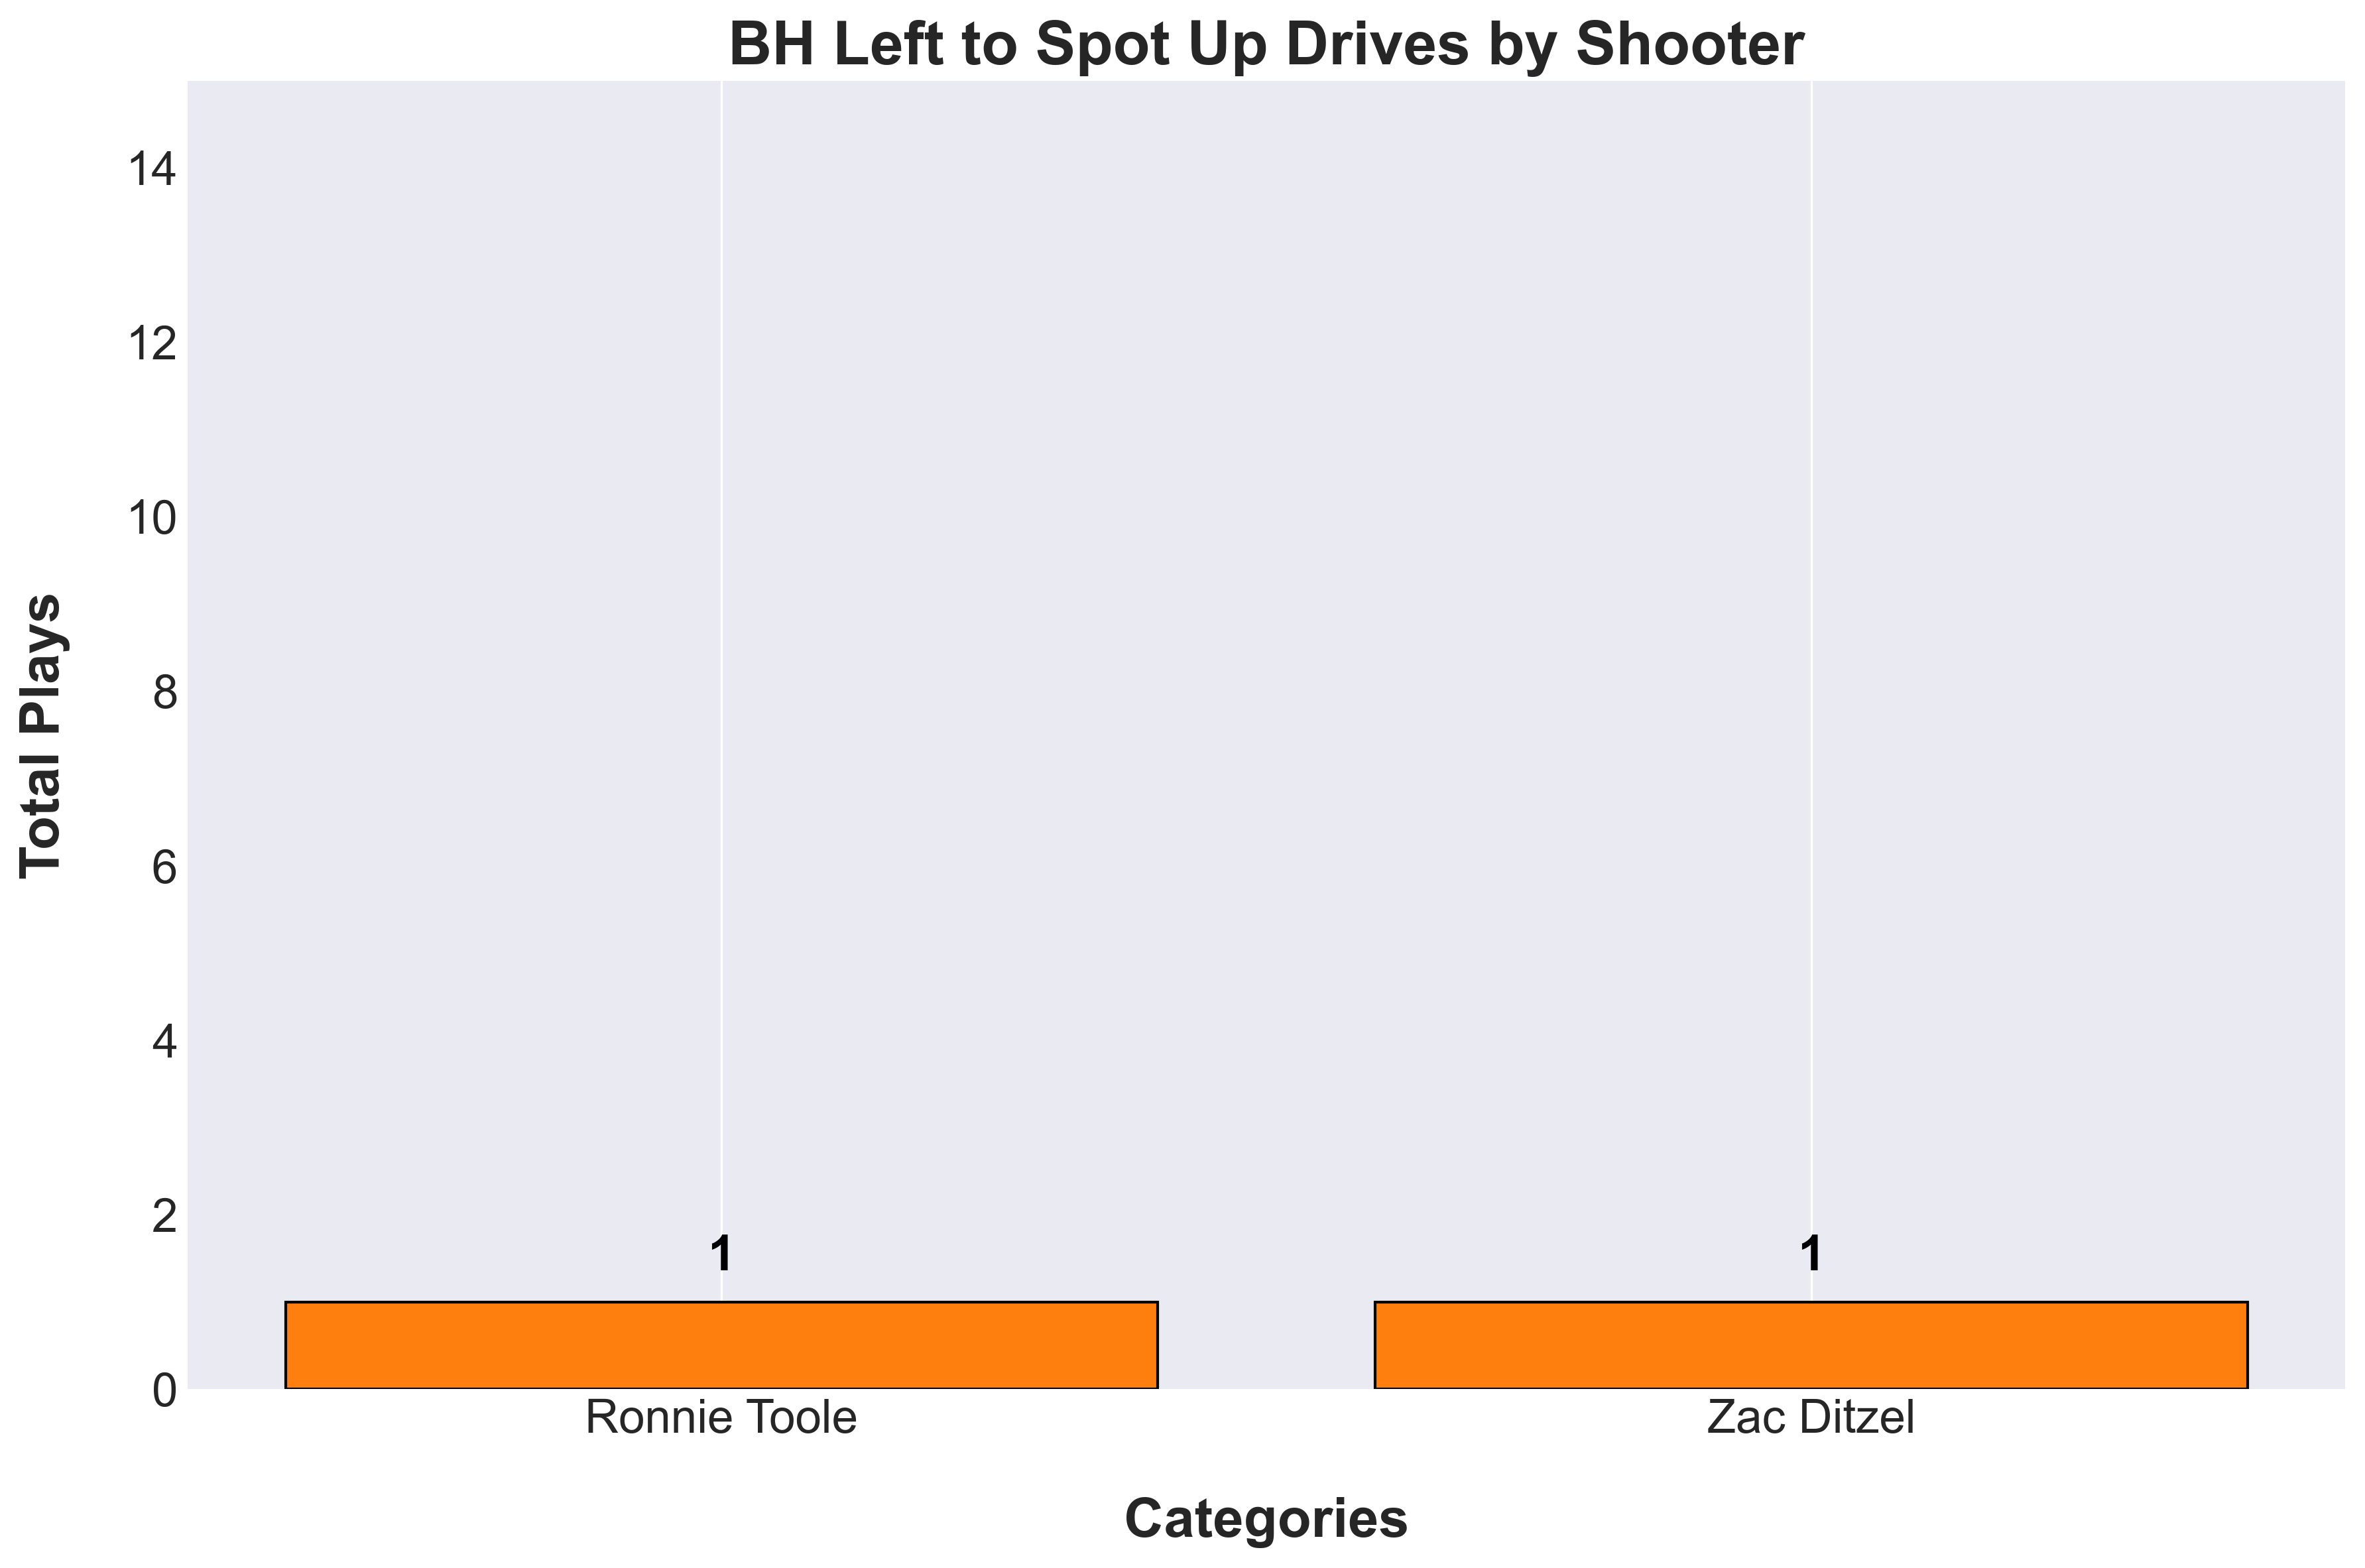
\includegraphics[width=\textwidth, height=.14\textheight]{images/PNR_PassLeftDrivesPlayer_Freq.png} % Adjust the width of the image to fit
    \end{minipage}
\end{table}

\vspace{-1em} % Add vertical space before the line (optional)
%\hrule height 1pt width 1\textwidth % Adjust height and width
\vspace{-1em} % Add vertical space after the line (optional)

% BH Left -> Spot Up Shots Secondary Player Stats
\begin{table}[H]
    \raisebox{3em}{ % Adjust this value to shift the tables vertically
    \begin{minipage}[t]{0.6\textwidth} % Left side (table) takes 85% of the width
        \flushleft
        \centering % Centering the title and the table
        \text{BH Left - Spot Up Shots Player Statistics} % Title above the table in bold
        \vskip .25em % Adds vertical space between title and table
        \scalebox{.6}{ % Scale the entire table down by half
            \renewcommand{\arraystretch}{1.4} % Adjust the number to increase or decrease row spacing
            \begin{tabular}{
            >{\centering\arraybackslash}p{3cm} 
            >{\centering\arraybackslash}p{.75cm} 
            >{\centering\arraybackslash}p{.75cm} 
            >{\centering\arraybackslash}p{.75cm} 
            >{\centering\arraybackslash}p{.75cm}
            >{\centering\arraybackslash}p{.75cm} 
            >{\centering\arraybackslash}p{.75cm} 
            >{\centering\arraybackslash}p{.75cm} 
            >{\centering\arraybackslash}p{.75cm}
            >{\centering\arraybackslash}p{.75cm} 
            >{\centering\arraybackslash}p{.75cm}
            >{\centering\arraybackslash}p{.75cm}
            >{\centering\arraybackslash}p{.75cm} 
            >{\centering\arraybackslash}p{.75cm}}% Adjust column widths
            \toprule
            {\scriptsize \textbf{Player}} &
            {\scriptsize \textbf{Plays}} &
            {\scriptsize \textbf{3PA}} &
            {\scriptsize \textbf{3PM}} &
            {\scriptsize \textbf{3P\%}} & 
            {\scriptsize \textbf{MiA}} & 
            {\scriptsize \textbf{MiM}} &
            {\scriptsize \textbf{Mi\%}} &
            {\scriptsize \textbf{EFG\%}} &
            {\scriptsize \textbf{TO}} &
            {\scriptsize \textbf{Foul}} \\
            \midrule
            
                
            
                
            
                
            
                
            
                
            
                
            
                
            
                
            
                
            
                
            
                
            
                
            
                
            
                
            
                
                    
                        Brock Bowen & 
                        1 & 
                        1 & 
                        0 & 
                        - & 
                        0 & 
                        0 & 
                        - & 
                        - & 
                        0 & 
                        0 \\
                    
                        Brody Brown & 
                        1 & 
                        1 & 
                        0 & 
                        - & 
                        0 & 
                        0 & 
                        - & 
                        - & 
                        0 & 
                        0 \\
                    
                        Keegan Ocorr & 
                        1 & 
                        1 & 
                        0 & 
                        - & 
                        0 & 
                        0 & 
                        - & 
                        - & 
                        0 & 
                        0 \\
                    
                
            
                
            
                
            
                
            
                
            
                
            
                
            
                
            
                
            
                
            
                
            
                
            
                
            
                
            
                
            
                
            
                
            
                
            
                
            
                
            
                
            
                
            
                
            
                
            
            \bottomrule
        \end{tabular}
        } % End of \scalebox
    \end{minipage}
    } % End of raisebox, closing the adjustment
    \hfill % This adds some flexible space between the table and the image
    \begin{minipage}[c]{0.35\textwidth} % Right side (image) takes 10% of the width
        \flushright
        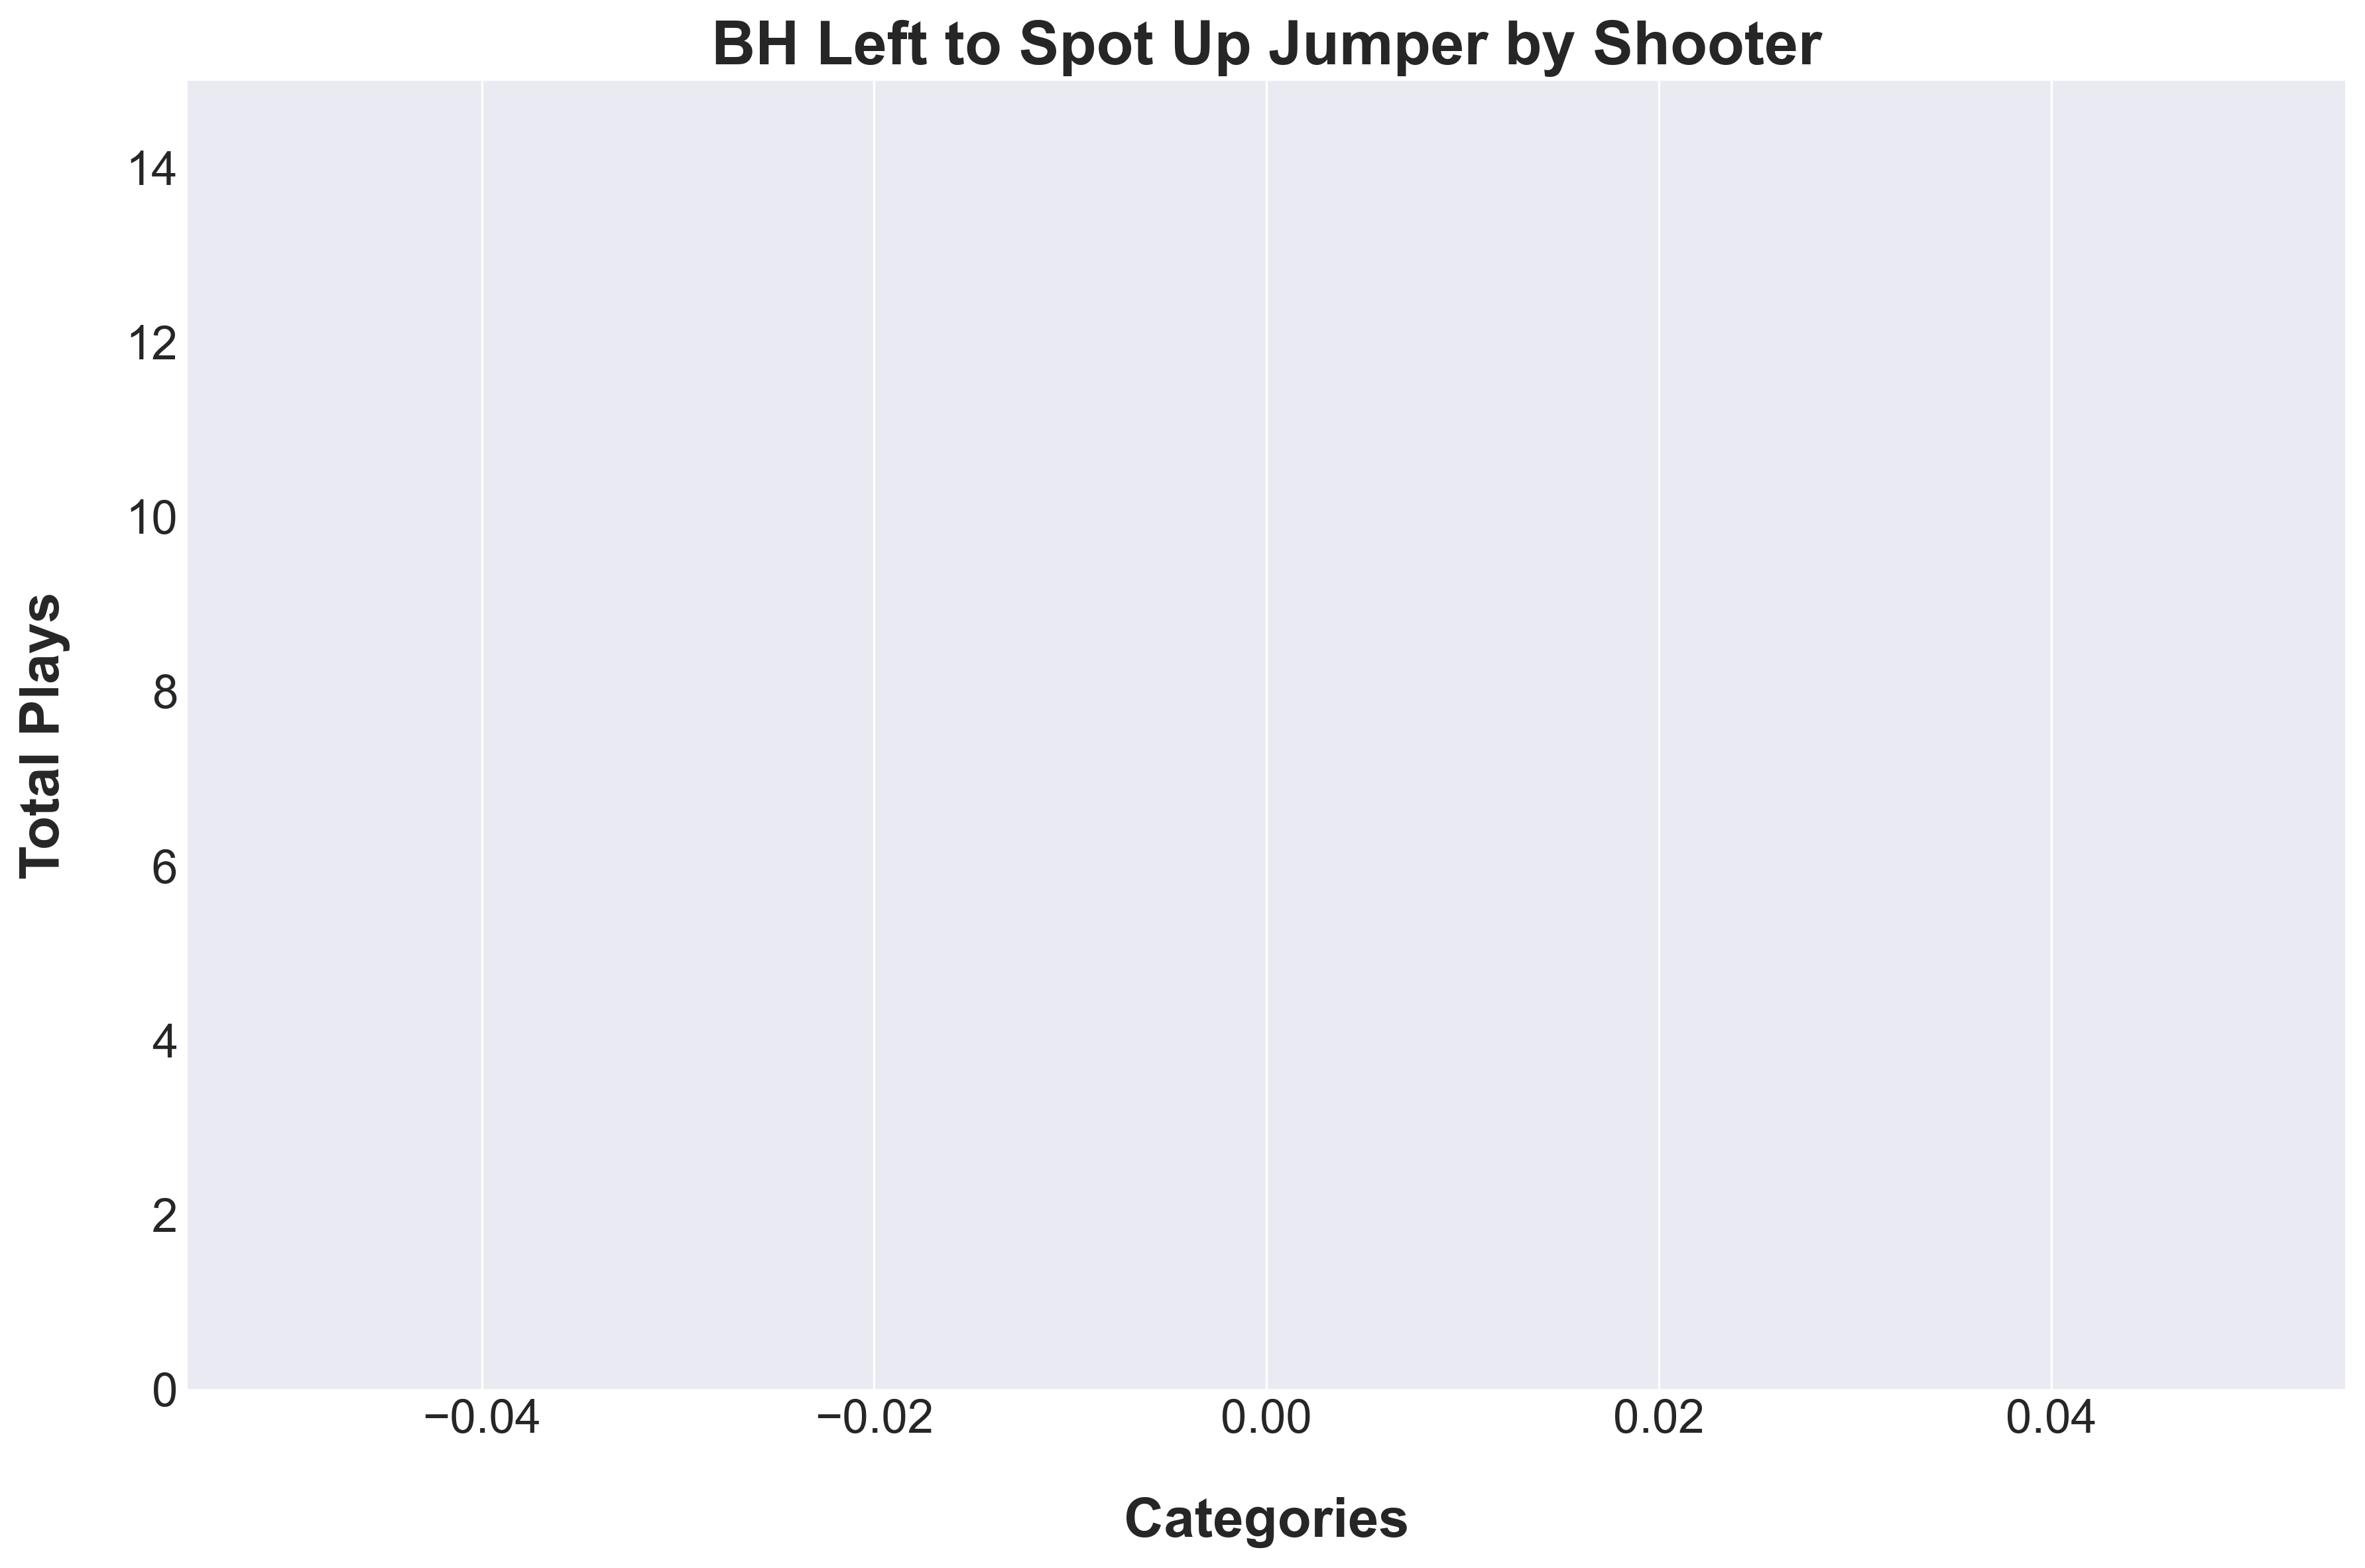
\includegraphics[width=\textwidth, height=.14\textheight]{images/PNR_PassLeftShotsPlayer_Freq.png} % Adjust the width of the image to fit
    \end{minipage}
\end{table}

\vspace{-1em} % Add vertical space before the line (optional)
%\hrule height 1pt width 1\textwidth % Adjust height and width
\vspace{-1em} % Add vertical space after the line (optional)

% BH Left -> Rollman Rolls Secondary Player Stats
\begin{table}[H]
    \raisebox{3em}{ % Adjust this value to shift the tables vertically
    \begin{minipage}[t]{0.6\textwidth} % Left side (table) takes 85% of the width
        \flushleft
        \centering % Centering the title and the table
        \text{BH Left - Rollman Rolls Player Statistics} % Title above the table in bold
        \vskip .25em % Adds vertical space between title and table
        \scalebox{.6}{ % Scale the entire table down by half
            \renewcommand{\arraystretch}{1.4} % Adjust the number to increase or decrease row spacing
            \begin{tabular}{
            >{\centering\arraybackslash}p{3cm} 
            >{\centering\arraybackslash}p{.75cm} 
            >{\centering\arraybackslash}p{.75cm} 
            >{\centering\arraybackslash}p{.75cm} 
            >{\centering\arraybackslash}p{.75cm}
            >{\centering\arraybackslash}p{.75cm} 
            >{\centering\arraybackslash}p{.75cm}
            >{\centering\arraybackslash}p{.75cm}
            >{\centering\arraybackslash}p{.75cm} 
            >{\centering\arraybackslash}p{.75cm}}% Adjust column widths
            \toprule
            {\scriptsize \textbf{Player}} &
            {\scriptsize \textbf{Plays}} &
            {\scriptsize \textbf{2PA}} & 
            {\scriptsize \textbf{2PM}} & 
            {\scriptsize \textbf{2P\%}} & 
            {\scriptsize \textbf{MiA}} & 
            {\scriptsize \textbf{MiM}} &
            {\scriptsize \textbf{Mi\%}} &
            {\scriptsize \textbf{TO}} &
            {\scriptsize \textbf{Foul}} \\
            \midrule
            
                
            
                
            
                
            
                
            
                
            
                
            
                
            
                
            
                
            
                
            
                
            
                
            
                
            
                
            
                
            
                
                    
                        Kenny Wilburn & 
                        2 & 
                        2 & 
                        1 & 
                        - & 
                        0 & 
                        0 & 
                        - & 
                        0 & 
                        0 \\
                    
                
            
                
            
                
            
                
            
                
            
                
            
                
            
                
            
                
            
                
            
                
            
                
            
                
            
                
            
                
            
                
            
                
            
                
            
                
            
                
            
                
            
                
            
                
            

            \bottomrule
        \end{tabular}
        } % End of \scalebox
    \end{minipage}
    } % End of raisebox, closing the adjustment
    \hfill % This adds some flexible space between the table and the image
    \begin{minipage}[c]{0.35\textwidth} % Right side (image) takes 10% of the width
        \flushright
        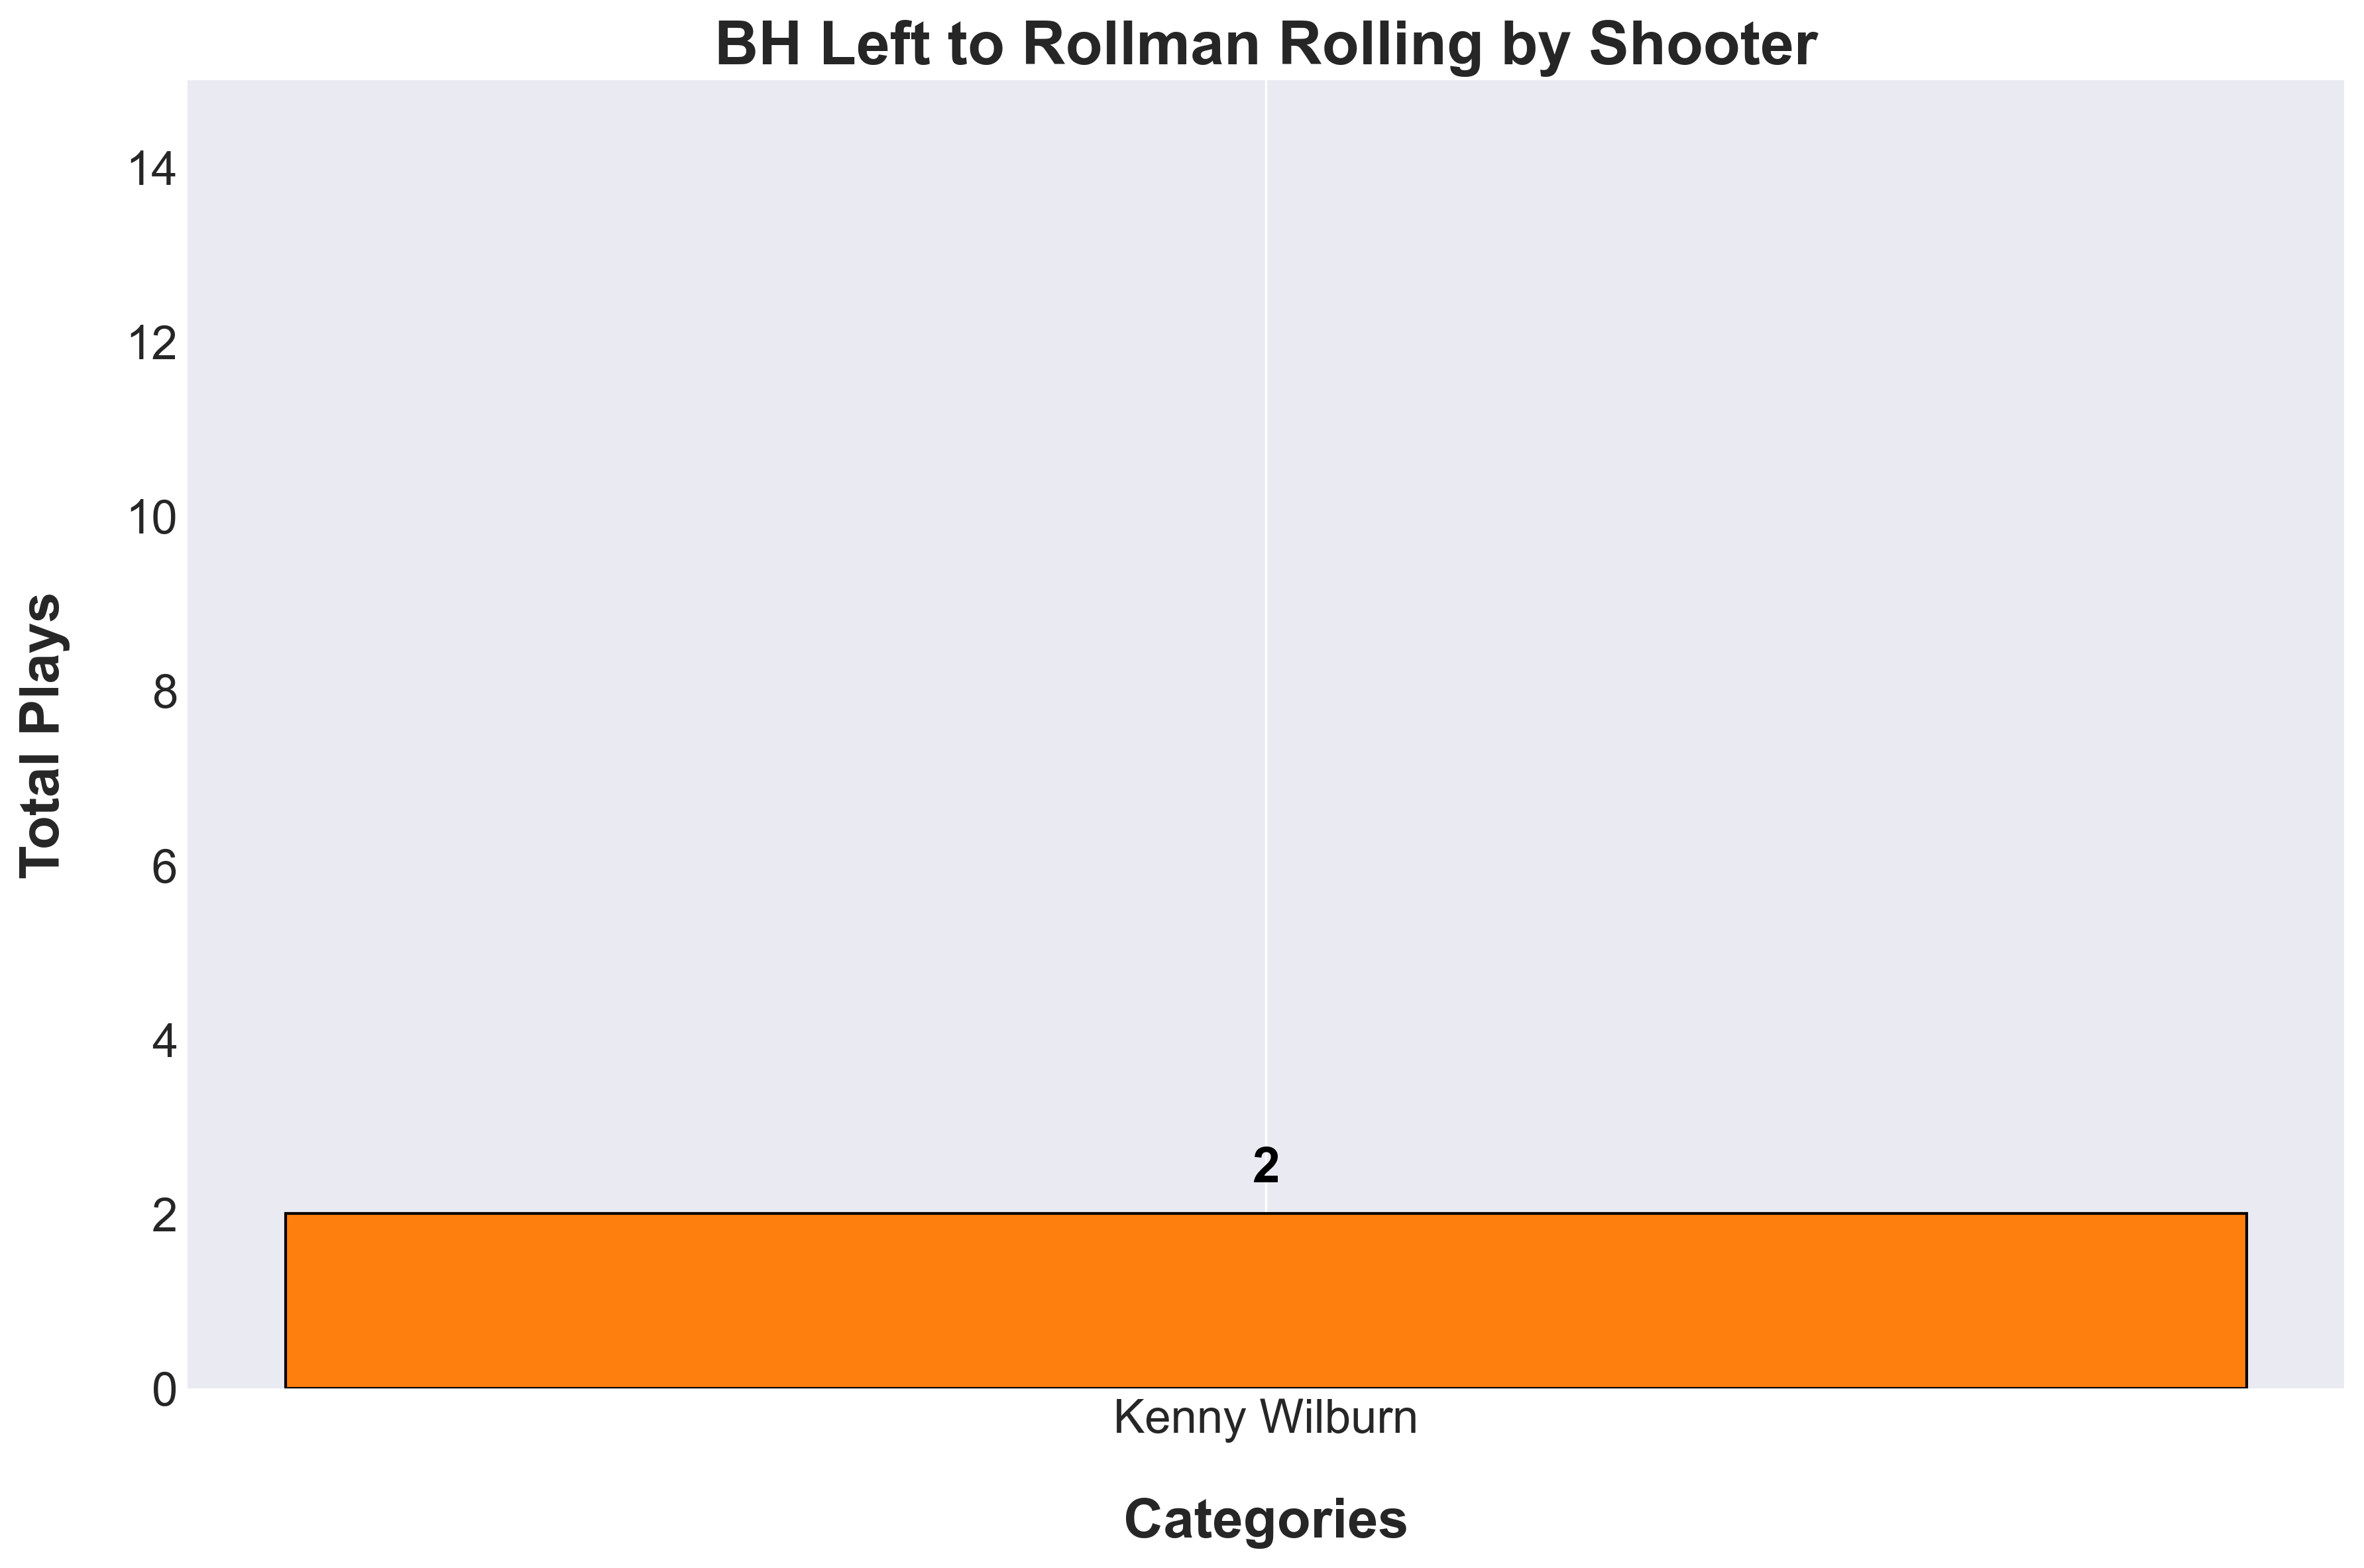
\includegraphics[width=\textwidth, height=.14\textheight]{images/PNR_PassLeftRollsPlayer_Freq.png} % Adjust the width of the image to fit
    \end{minipage}
\end{table}

\vspace{-1em} % Add vertical space before the line (optional)
%\hrule height 1pt width 1\textwidth % Adjust height and width
\vspace{-1em} % Add vertical space after the line (optional)

% BH Left -> Rollman Slips Secondary Player Stats
\begin{table}[H]
    \raisebox{3em}{ % Adjust this value to shift the tables vertically
    \begin{minipage}[t]{0.6\textwidth} % Left side (table) takes 85% of the width
        \flushleft
        \centering % Centering the title and the table
        \text{BH Left - Rollman Slips Player Statistics} % Title above the table in bold
        \vskip .25em % Adds vertical space between title and table
        \scalebox{.55}{ % Scale the entire table down by half
            \renewcommand{\arraystretch}{1.4} % Adjust the number to increase or decrease row spacing
            \begin{tabular}{
            >{\centering\arraybackslash}p{3cm} 
            >{\centering\arraybackslash}p{.75cm} 
            >{\centering\arraybackslash}p{.75cm} 
            >{\centering\arraybackslash}p{.75cm} 
            >{\centering\arraybackslash}p{.75cm}
            >{\centering\arraybackslash}p{.75cm} 
            >{\centering\arraybackslash}p{.75cm} 
            >{\centering\arraybackslash}p{.75cm} 
            >{\centering\arraybackslash}p{.75cm}
            >{\centering\arraybackslash}p{.75cm} 
            >{\centering\arraybackslash}p{.75cm}
            >{\centering\arraybackslash}p{.75cm}
            >{\centering\arraybackslash}p{.75cm} 
            >{\centering\arraybackslash}p{.75cm}}% Adjust column widths
            \toprule
            {\scriptsize \textbf{Player}} &
            {\scriptsize \textbf{Plays}} &
            {\scriptsize \textbf{3PA}} &
            {\scriptsize \textbf{3PM}} &
            {\scriptsize \textbf{3P\%}} & 
            {\scriptsize \textbf{2PA}} & 
            {\scriptsize \textbf{2PM}} & 
            {\scriptsize \textbf{2P\%}} & 
            {\scriptsize \textbf{MiA}} & 
            {\scriptsize \textbf{MiM}} &
            {\scriptsize \textbf{Mi\%}} &
            {\scriptsize \textbf{EFG\%}} &
            {\scriptsize \textbf{TO}} &
            {\scriptsize \textbf{Foul}} \\
            \midrule
            
                
            
                
            
                
            
                
            
                
            
                
            
                
            
                
            
                
            
                
            
                
            
                
            
                
            
                
            
                
            
                
            
                
                    
                
            
                
            
                
            
                
            
                
            
                
            
                
            
                
            
                
            
                
            
                
            
                
            
                
            
                
            
                
            
                
            
                
            
                
            
                
            
                
            
                
            
                
            

            \bottomrule
        \end{tabular}
        } % End of \scalebox
    \end{minipage}
    } % End of raisebox, closing the adjustment
    \hfill % This adds some flexible space between the table and the image
    \begin{minipage}[c]{0.35\textwidth} % Right side (image) takes 10% of the width
        \flushright
        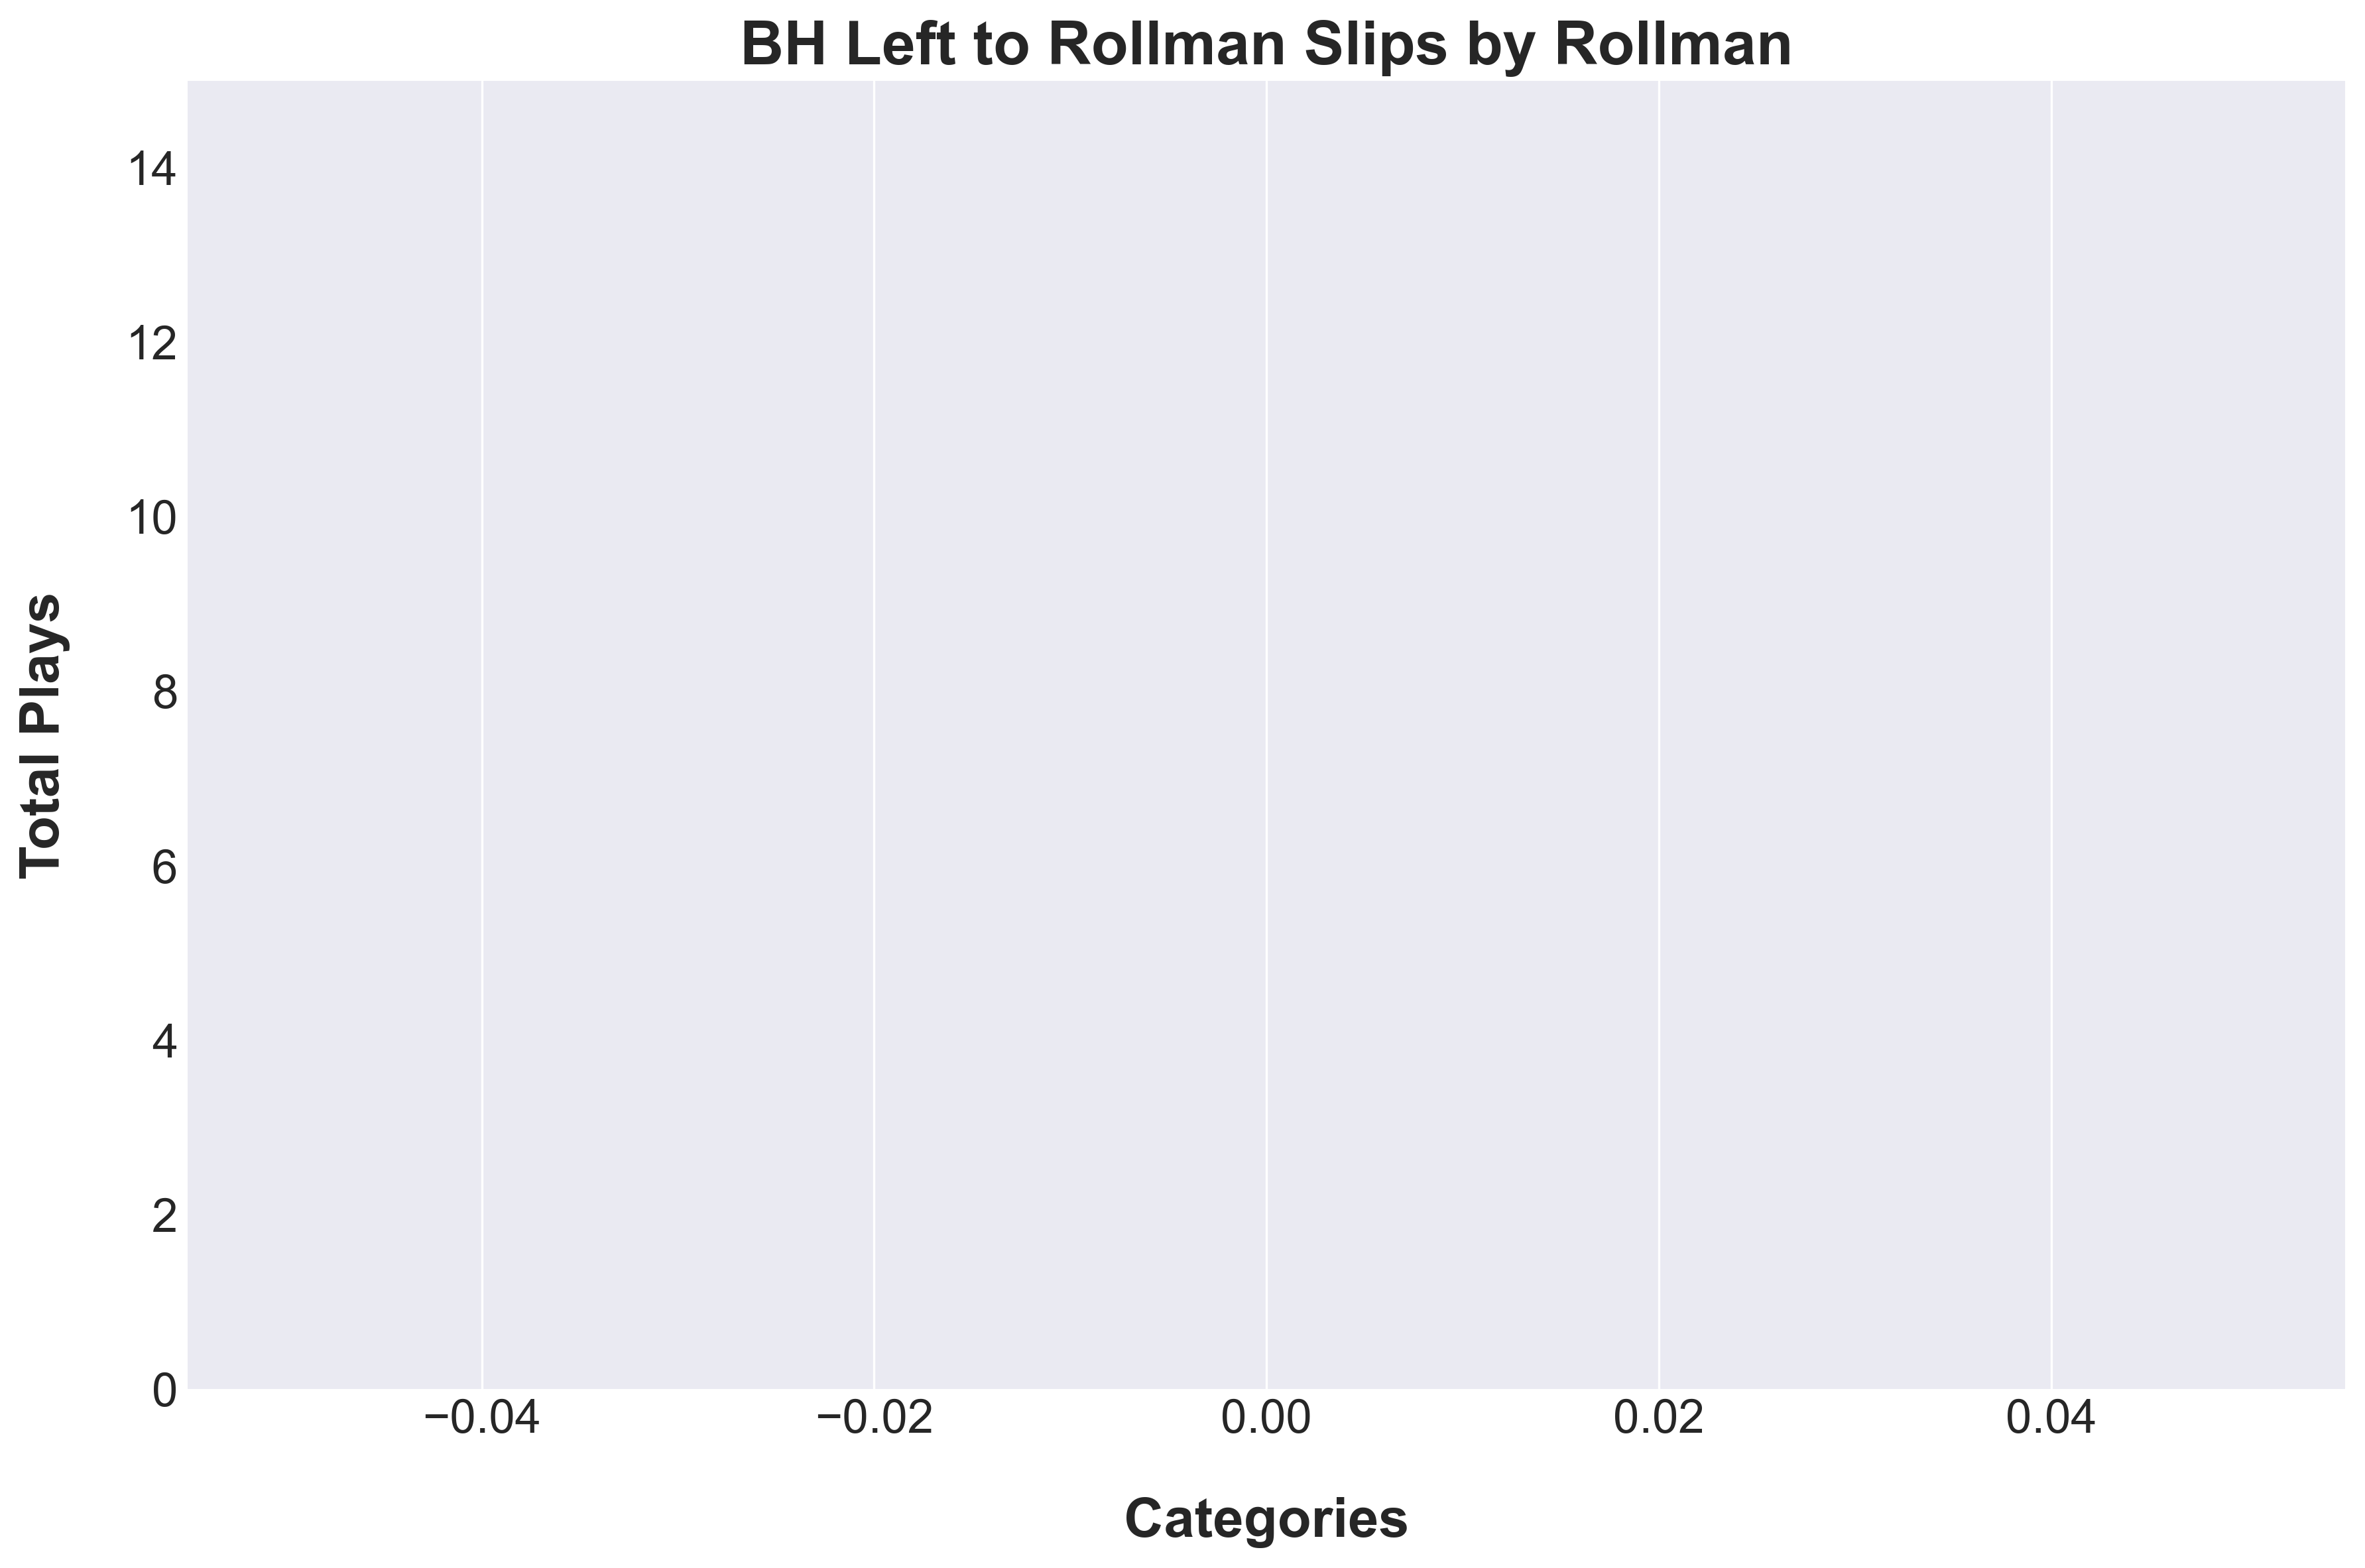
\includegraphics[width=\textwidth, height=.14\textheight]{images/PNR_PassLeftSlipsPlayer_Freq.png} % Adjust the width of the image to fit
    \end{minipage}
\end{table}

\vspace{-1em} % Add vertical space before the line (optional)
%\hrule height 1pt width 1\textwidth % Adjust height and width
\vspace{-1em} % Add vertical space after the line (optional)

% BH Left -> Rollman Pops Secondary Player Stats
\begin{table}[H]
    \raisebox{3em}{ % Adjust this value to shift the tables vertically
    \begin{minipage}[t]{0.6\textwidth} % Left side (table) takes 85% of the width
        \flushleft
        \centering % Centering the title and the table
        \text{BH Left - Rollman Pops Player Statistics} % Title above the table in bold
        \vskip .25em % Adds vertical space between title and table
        \scalebox{.55}{ % Scale the entire table down by half
            \renewcommand{\arraystretch}{1.4} % Adjust the number to increase or decrease row spacing
            \begin{tabular}{
            >{\centering\arraybackslash}p{3cm} 
            >{\centering\arraybackslash}p{.75cm} 
            >{\centering\arraybackslash}p{.75cm} 
            >{\centering\arraybackslash}p{.75cm} 
            >{\centering\arraybackslash}p{.75cm}
            >{\centering\arraybackslash}p{.75cm} 
            >{\centering\arraybackslash}p{.75cm} 
            >{\centering\arraybackslash}p{.75cm} 
            >{\centering\arraybackslash}p{.75cm}
            >{\centering\arraybackslash}p{.75cm} 
            >{\centering\arraybackslash}p{.75cm}
            >{\centering\arraybackslash}p{.75cm}
            >{\centering\arraybackslash}p{.75cm} 
            >{\centering\arraybackslash}p{.75cm}}% Adjust column widths
            \toprule
            {\scriptsize \textbf{Player}} &
            {\scriptsize \textbf{Plays}} &
            {\scriptsize \textbf{3PA}} &
            {\scriptsize \textbf{3PM}} &
            {\scriptsize \textbf{3P\%}} & 
            {\scriptsize \textbf{2PA}} & 
            {\scriptsize \textbf{2PM}} & 
            {\scriptsize \textbf{2P\%}} & 
            {\scriptsize \textbf{MiA}} & 
            {\scriptsize \textbf{MiM}} &
            {\scriptsize \textbf{Mi\%}} &
            {\scriptsize \textbf{EFG\%}} &
            {\scriptsize \textbf{TO}} &
            {\scriptsize \textbf{Foul}} \\
            \midrule
            
                
            
                
            
                
            
                
            
                
            
                
            
                
            
                
            
                
            
                
            
                
            
                
            
                
            
                
            
                
            
                
            
                
            
                
                    
                        Josiah Turner & 
                        1 & 
                        0 & 
                        0 & 
                        - & 
                        1 & 
                        0 & 
                        - & 
                        0 & 
                        0 & 
                        - & 
                        - & 
                        0 & 
                        0 \\
                    
                
            
                
            
                
            
                
            
                
            
                
            
                
            
                
            
                
            
                
            
                
            
                
            
                
            
                
            
                
            
                
            
                
            
                
            
                
            
                
            
                
            


            \bottomrule
        \end{tabular}
        } % End of \scalebox
    \end{minipage}
    } % End of raisebox, closing the adjustment
    \hfill % This adds some flexible space between the table and the image
    \begin{minipage}[c]{0.35\textwidth} % Right side (image) takes 10% of the width
        \flushright
        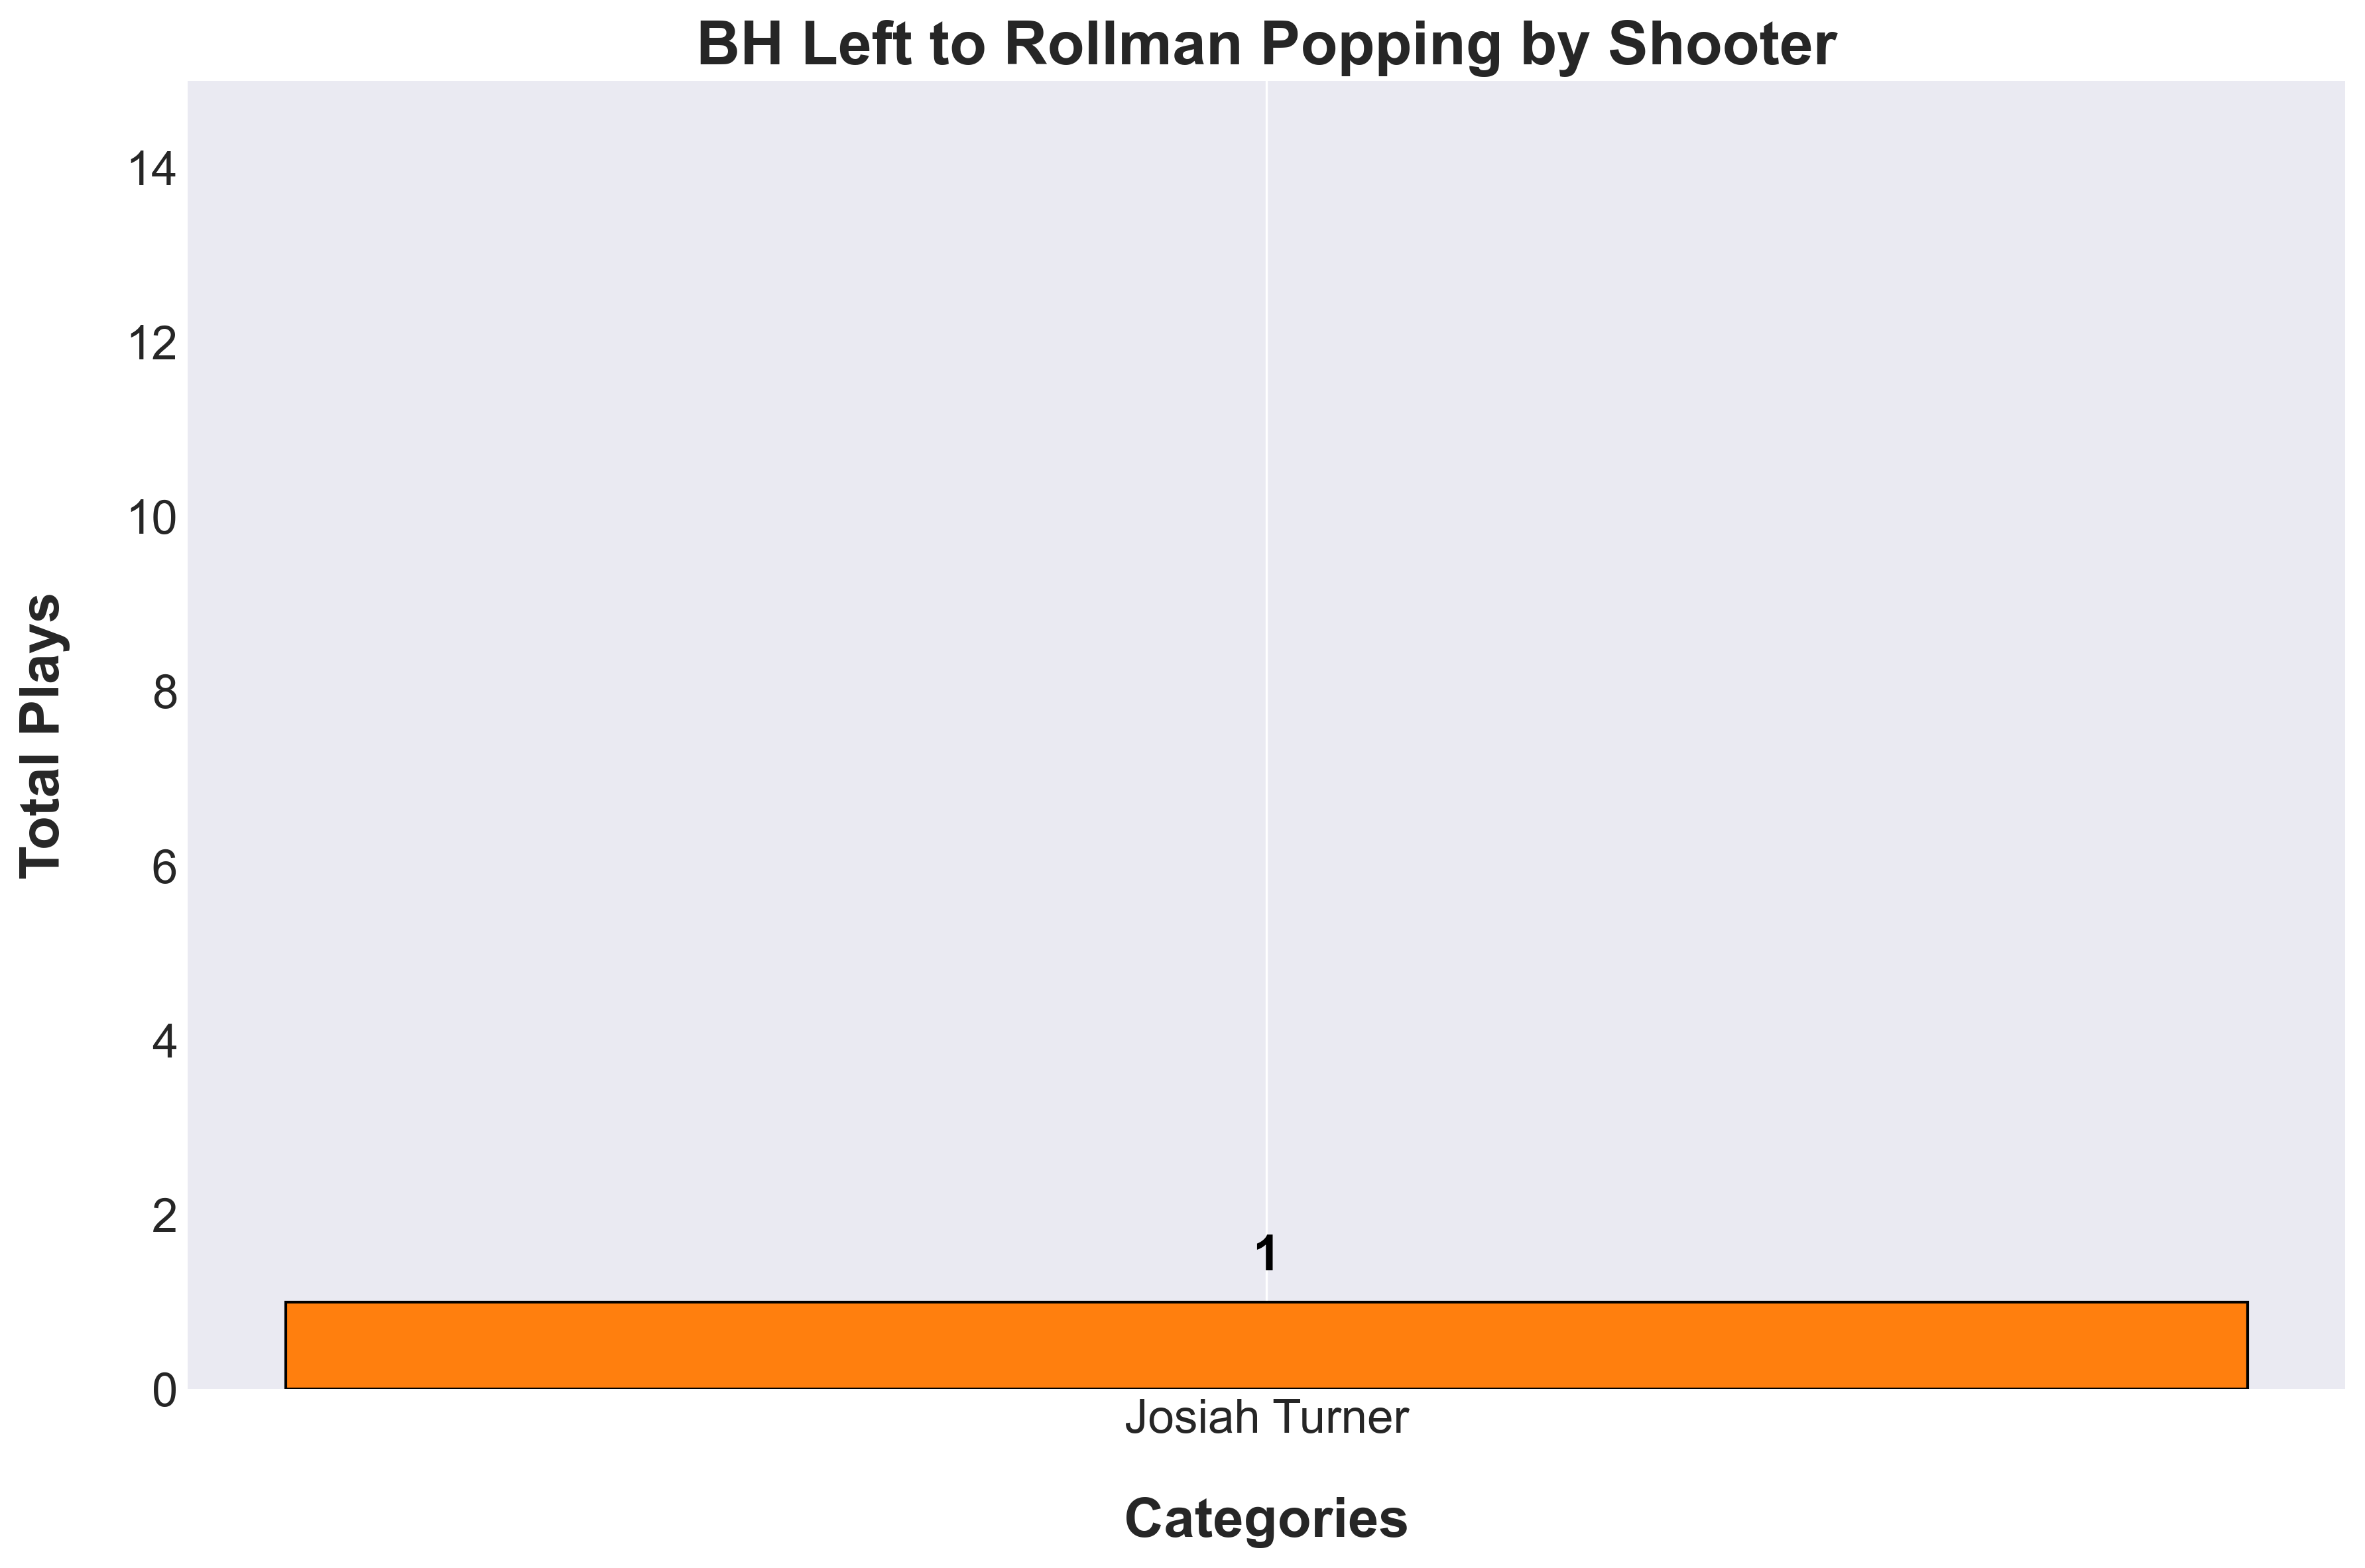
\includegraphics[width=\textwidth, height=.14\textheight]{images/PNR_PassLeftPopsPlayer_Freq.png} % Adjust the width of the image to fit
    \end{minipage}
\end{table}

\vspace{-1em} % Add vertical space before the line (optional)
\hrule height 1pt width 1\textwidth % Adjust height and width
\vspace{1em} % Add vertical space after the line (optional)

\subsubsection{BH Right PNR Passer Statistics}

% BH Right -> Cuts Secondary Player Stats
\begin{table}[H]
    \raisebox{3em}{ % Adjust this value to shift the tables vertically
    \begin{minipage}[t]{0.6\textwidth} % Left side (table) takes 85% of the width
        \flushleft
        \centering % Centering the title and the table
        \text{BH Right - Cuts Player Statistics} % Title above the table in bold
        \vskip .25em % Adds vertical space between title and table
        \scalebox{.6}{ % Scale the entire table down by half
            \renewcommand{\arraystretch}{1.4} % Adjust the number to increase or decrease row spacing
            \begin{tabular}{
            >{\centering\arraybackslash}p{3cm} 
            >{\centering\arraybackslash}p{.75cm} 
            >{\centering\arraybackslash}p{.75cm} 
            >{\centering\arraybackslash}p{.75cm} 
            >{\centering\arraybackslash}p{.75cm}
            >{\centering\arraybackslash}p{.75cm} 
            >{\centering\arraybackslash}p{.75cm}
            >{\centering\arraybackslash}p{.75cm}
            >{\centering\arraybackslash}p{.75cm} 
            >{\centering\arraybackslash}p{.75cm}}% Adjust column widths
            \toprule
            {\scriptsize \textbf{Player}} &
            {\scriptsize \textbf{Plays}} &
            {\scriptsize \textbf{2PA}} & 
            {\scriptsize \textbf{2PM}} & 
            {\scriptsize \textbf{2P\%}} & 
            {\scriptsize \textbf{MiA}} & 
            {\scriptsize \textbf{MiM}} &
            {\scriptsize \textbf{Mi\%}} &
            {\scriptsize \textbf{TO}} &
            {\scriptsize \textbf{Foul}} \\
            \midrule
            
                
            
                
            
                
            
                
            
                
            
                
            
                
            
                
            
                
            
                
            
                
            
                
            
                
            
                
            
                
            
                
            
                
            
                
            
                
                    
                        Nolan Smih & 
                        1 & 
                        1 & 
                        1 & 
                        - & 
                        0 & 
                        0 & 
                        - & 
                        0 & 
                        0 \\
                    
                
            
                
            
                
            
                
            
                
            
                
            
                
            
                
            
                
            
                
            
                
            
                
            
                
            
                
            
                
            
                
            
                
            
                
            
                
            
                
            

            \bottomrule
        \end{tabular}
        } % End of \scalebox
    \end{minipage}
    } % End of raisebox, closing the adjustment
    \hfill % This adds some flexible space between the table and the image
    \begin{minipage}[c]{0.35\textwidth} % Right side (image) takes 10% of the width
        \flushright
        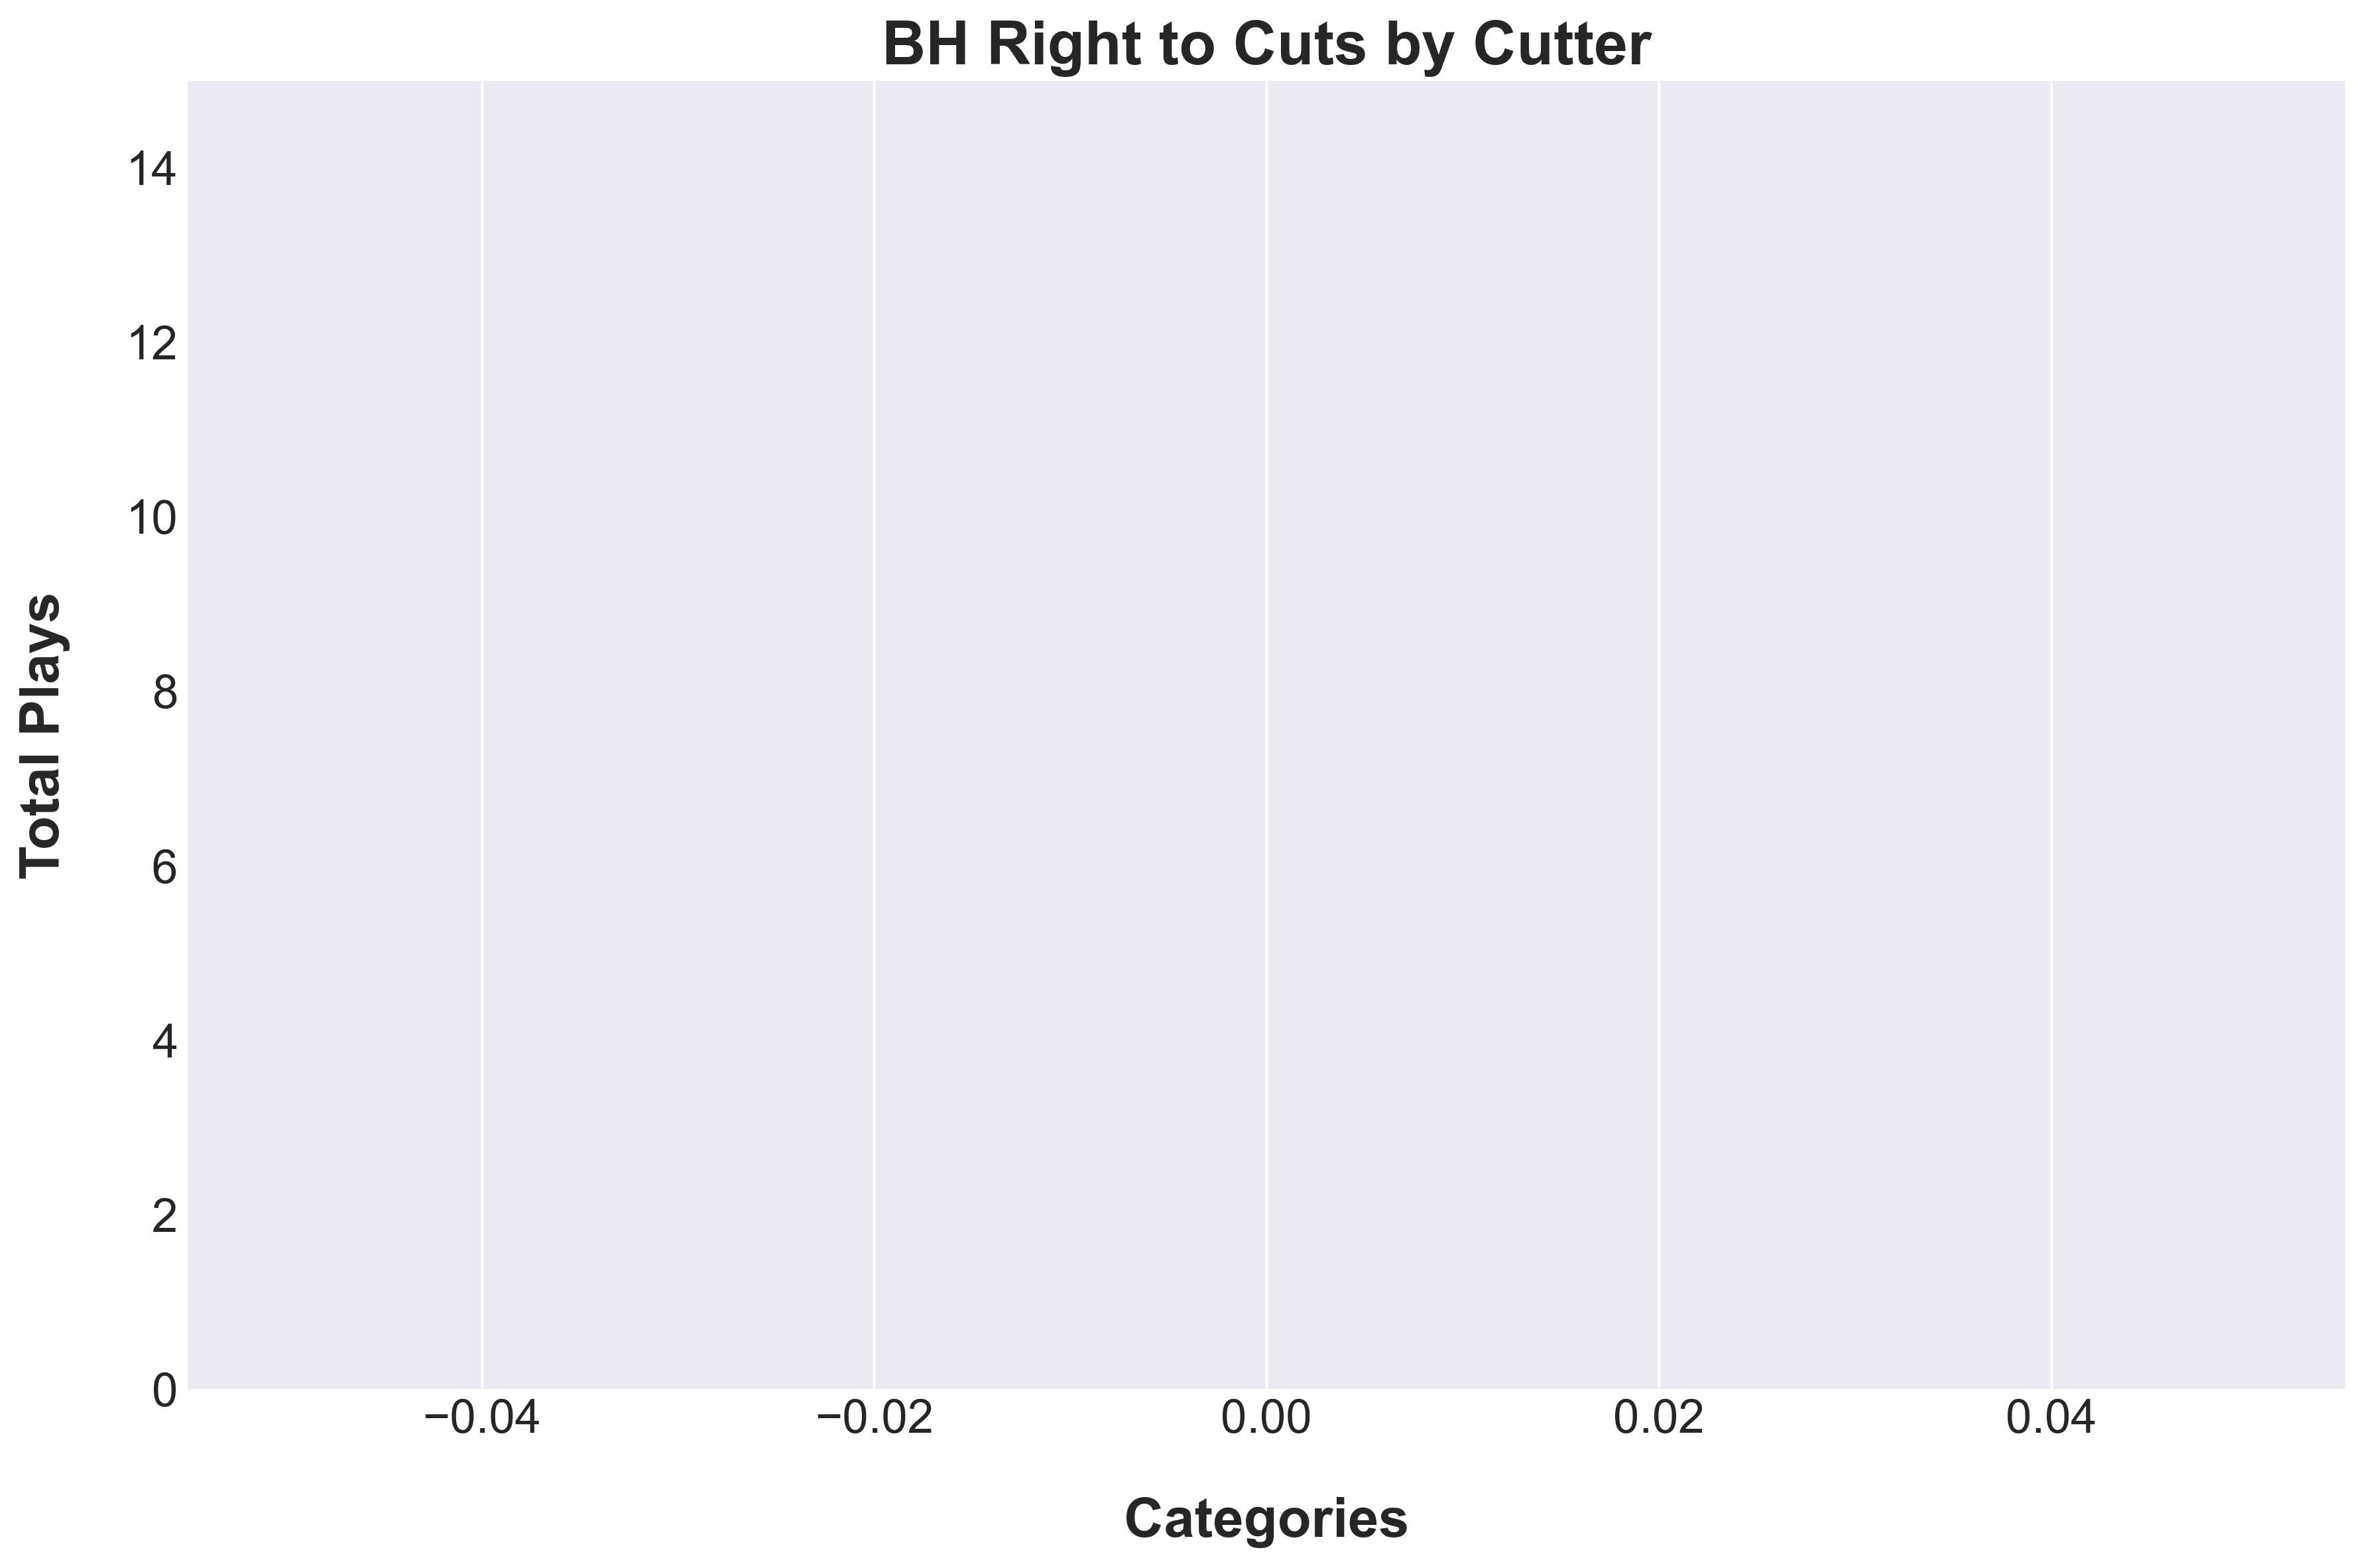
\includegraphics[width=\textwidth, height=.14\textheight]{images/PNR_PassRightCutsPlayer_Freq.png} % Adjust the width of the image to fit
    \end{minipage}
\end{table}

\vspace{-1em} % Add vertical space before the line (optional)
%\hrule height 1pt width 1\textwidth % Adjust height and width
\vspace{-1em} % Add vertical space after the line (optional)

% BH Right -> Spot Up Drives Secondary Player Stats
\begin{table}[H]
    \raisebox{3em}{ % Adjust this value to shift the tables vertically
    \begin{minipage}[t]{0.6\textwidth} % Left side (table) takes 85% of the width
        \flushleft
        \centering % Centering the title and the table
        \text{BH Right - Spot Up Drives Player Statistics} % Title above the table in bold
        \vskip .25em % Adds vertical space between title and table
        \scalebox{.55}{ % Scale the entire table down by half
            \renewcommand{\arraystretch}{1.4} % Adjust the number to increase or decrease row spacing
            \begin{tabular}{
            >{\centering\arraybackslash}p{3cm} 
            >{\centering\arraybackslash}p{.75cm} 
            >{\centering\arraybackslash}p{.75cm} 
            >{\centering\arraybackslash}p{.75cm} 
            >{\centering\arraybackslash}p{.75cm}
            >{\centering\arraybackslash}p{.75cm} 
            >{\centering\arraybackslash}p{.75cm} 
            >{\centering\arraybackslash}p{.75cm} 
            >{\centering\arraybackslash}p{.75cm}
            >{\centering\arraybackslash}p{.75cm} 
            >{\centering\arraybackslash}p{.75cm}
            >{\centering\arraybackslash}p{.75cm}
            >{\centering\arraybackslash}p{.75cm} 
            >{\centering\arraybackslash}p{.75cm}}% Adjust column widths
            \toprule
            {\scriptsize \textbf{Player}} &
            {\scriptsize \textbf{Plays}} &
            {\scriptsize \textbf{3PA}} &
            {\scriptsize \textbf{3PM}} &
            {\scriptsize \textbf{3P\%}} & 
            {\scriptsize \textbf{2PA}} & 
            {\scriptsize \textbf{2PM}} & 
            {\scriptsize \textbf{2P\%}} & 
            {\scriptsize \textbf{MiA}} & 
            {\scriptsize \textbf{MiM}} &
            {\scriptsize \textbf{Mi\%}} &
            {\scriptsize \textbf{EFG\%}} &
            {\scriptsize \textbf{TO}} &
            {\scriptsize \textbf{Foul}} \\
            \midrule
            
                
            
                
            
                
            
                
            
                
            
                
            
                
            
                
            
                
            
                
            
                
            
                
            
                
            
                
            
                
            
                
            
                
            
                
            
                
            
                
                    
                        Brock Bowen & 
                        1 & 
                        0 & 
                        0 & 
                        - & 
                        0 & 
                        0 & 
                        - & 
                        0 & 
                        0 & 
                        - & 
                        - & 
                        1 & 
                        0 \\
                    
                        Chase Dickens & 
                        1 & 
                        1 & 
                        0 & 
                        - & 
                        0 & 
                        0 & 
                        - & 
                        0 & 
                        0 & 
                        - & 
                        - & 
                        0 & 
                        0 \\
                    
                        Mark Osime & 
                        1 & 
                        0 & 
                        0 & 
                        - & 
                        0 & 
                        0 & 
                        - & 
                        0 & 
                        0 & 
                        - & 
                        - & 
                        0 & 
                        1 \\
                    
                
            
                
            
                
            
                
            
                
            
                
            
                
            
                
            
                
            
                
            
                
            
                
            
                
            
                
            
                
            
                
            
                
            
                
            
                
            

            \bottomrule
        \end{tabular}
        } % End of \scalebox
    \end{minipage}
    } % End of raisebox, closing the adjustment
    \hfill % This adds some flexible space between the table and the image
    \begin{minipage}[c]{0.35\textwidth} % Right side (image) takes 10% of the width
        \flushright
        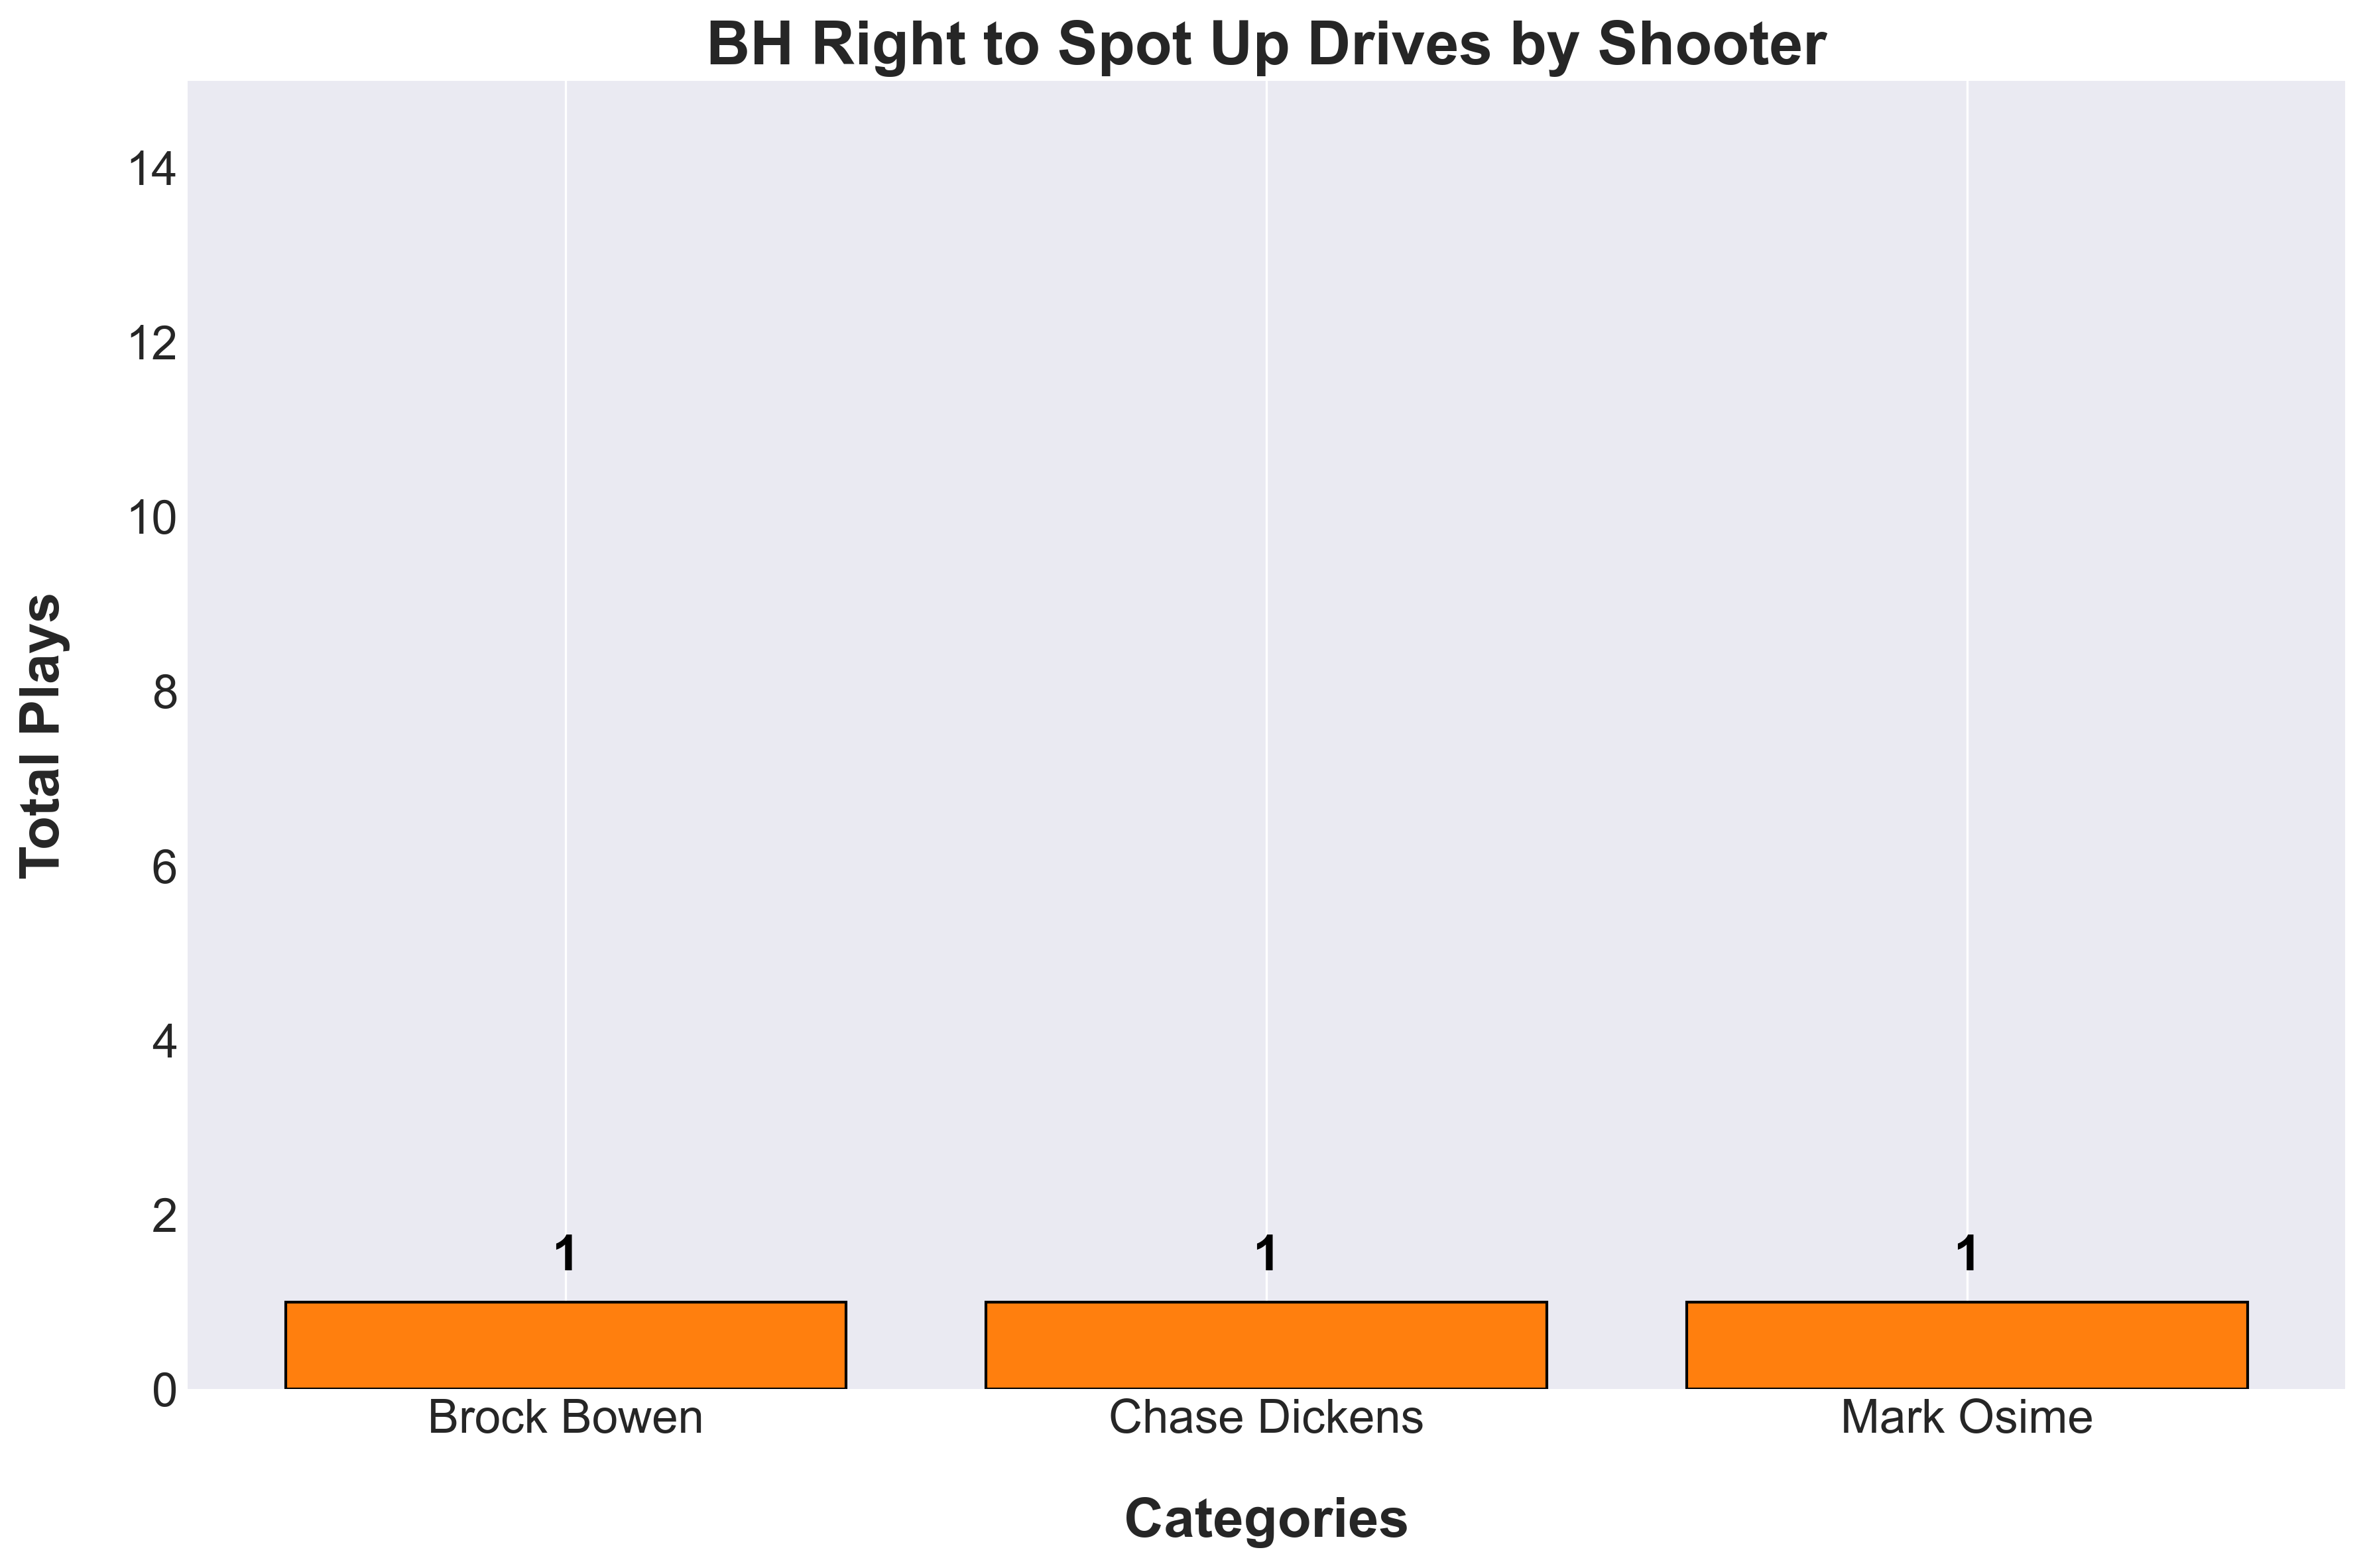
\includegraphics[width=\textwidth, height=.14\textheight]{images/PNR_PassRightDrivesPlayer_Freq.png} % Adjust the width of the image to fit
    \end{minipage}
\end{table}

\vspace{-1em} % Add vertical space before the line (optional)
%\hrule height 1pt width 1\textwidth % Adjust height and width
\vspace{-1em} % Add vertical space after the line (optional)

% BH Right -> Spot Up Shots Secondary Player Stats
\begin{table}[H]
    \raisebox{3em}{ % Adjust this value to shift the tables vertically
    \begin{minipage}[t]{0.6\textwidth} % Left side (table) takes 85% of the width
        \flushleft
        \centering % Centering the title and the table
        \text{BH Right - Spot Up Shots Player Statistics} % Title above the table in bold
        \vskip .25em % Adds vertical space between title and table
        \scalebox{.6}{ % Scale the entire table down by half
            \renewcommand{\arraystretch}{1.4} % Adjust the number to increase or decrease row spacing
            \begin{tabular}{
            >{\centering\arraybackslash}p{3cm} 
            >{\centering\arraybackslash}p{.75cm} 
            >{\centering\arraybackslash}p{.75cm} 
            >{\centering\arraybackslash}p{.75cm} 
            >{\centering\arraybackslash}p{.75cm}
            >{\centering\arraybackslash}p{.75cm} 
            >{\centering\arraybackslash}p{.75cm} 
            >{\centering\arraybackslash}p{.75cm}
            >{\centering\arraybackslash}p{.75cm}
            >{\centering\arraybackslash}p{.75cm} 
            >{\centering\arraybackslash}p{.75cm}}% Adjust column widths
            \toprule
            {\scriptsize \textbf{Player}} &
            {\scriptsize \textbf{Plays}} &
            {\scriptsize \textbf{3PA}} &
            {\scriptsize \textbf{3PM}} &
            {\scriptsize \textbf{3P\%}} & 
            {\scriptsize \textbf{MiA}} & 
            {\scriptsize \textbf{MiM}} &
            {\scriptsize \textbf{Mi\%}} &
            {\scriptsize \textbf{EFG\%}} &
            {\scriptsize \textbf{TO}} &
            {\scriptsize \textbf{Foul}} \\
            \midrule
            
                
            
                
            
                
            
                
            
                
            
                
            
                
            
                
            
                
            
                
            
                
            
                
            
                
            
                
            
                
            
                
            
                
            
                
            
                
            
                
            
                
                    
                        Brock Bowen & 
                        2 & 
                        2 & 
                        1 & 
                        - & 
                        0 & 
                        0 & 
                        - & 
                        - & 
                        0 & 
                        0 \\
                    
                        Brody Brown & 
                        1 & 
                        1 & 
                        0 & 
                        - & 
                        0 & 
                        0 & 
                        - & 
                        - & 
                        0 & 
                        0 \\
                    
                        Keegan Ocorr & 
                        1 & 
                        1 & 
                        0 & 
                        - & 
                        0 & 
                        0 & 
                        - & 
                        - & 
                        0 & 
                        0 \\
                    
                        Kenny Wilburn & 
                        1 & 
                        0 & 
                        0 & 
                        - & 
                        1 & 
                        0 & 
                        - & 
                        - & 
                        0 & 
                        0 \\
                    
                        Zac Ditzel & 
                        1 & 
                        1 & 
                        0 & 
                        - & 
                        0 & 
                        0 & 
                        - & 
                        - & 
                        0 & 
                        0 \\
                    
                
            
                
            
                
            
                
            
                
            
                
            
                
            
                
            
                
            
                
            
                
            
                
            
                
            
                
            
                
            
                
            
                
            
                
            

            \bottomrule
        \end{tabular}
        } % End of \scalebox
    \end{minipage}
    } % End of raisebox, closing the adjustment
    \hfill % This adds some flexible space between the table and the image
    \begin{minipage}[c]{0.35\textwidth} % Right side (image) takes 10% of the width
        \flushright
        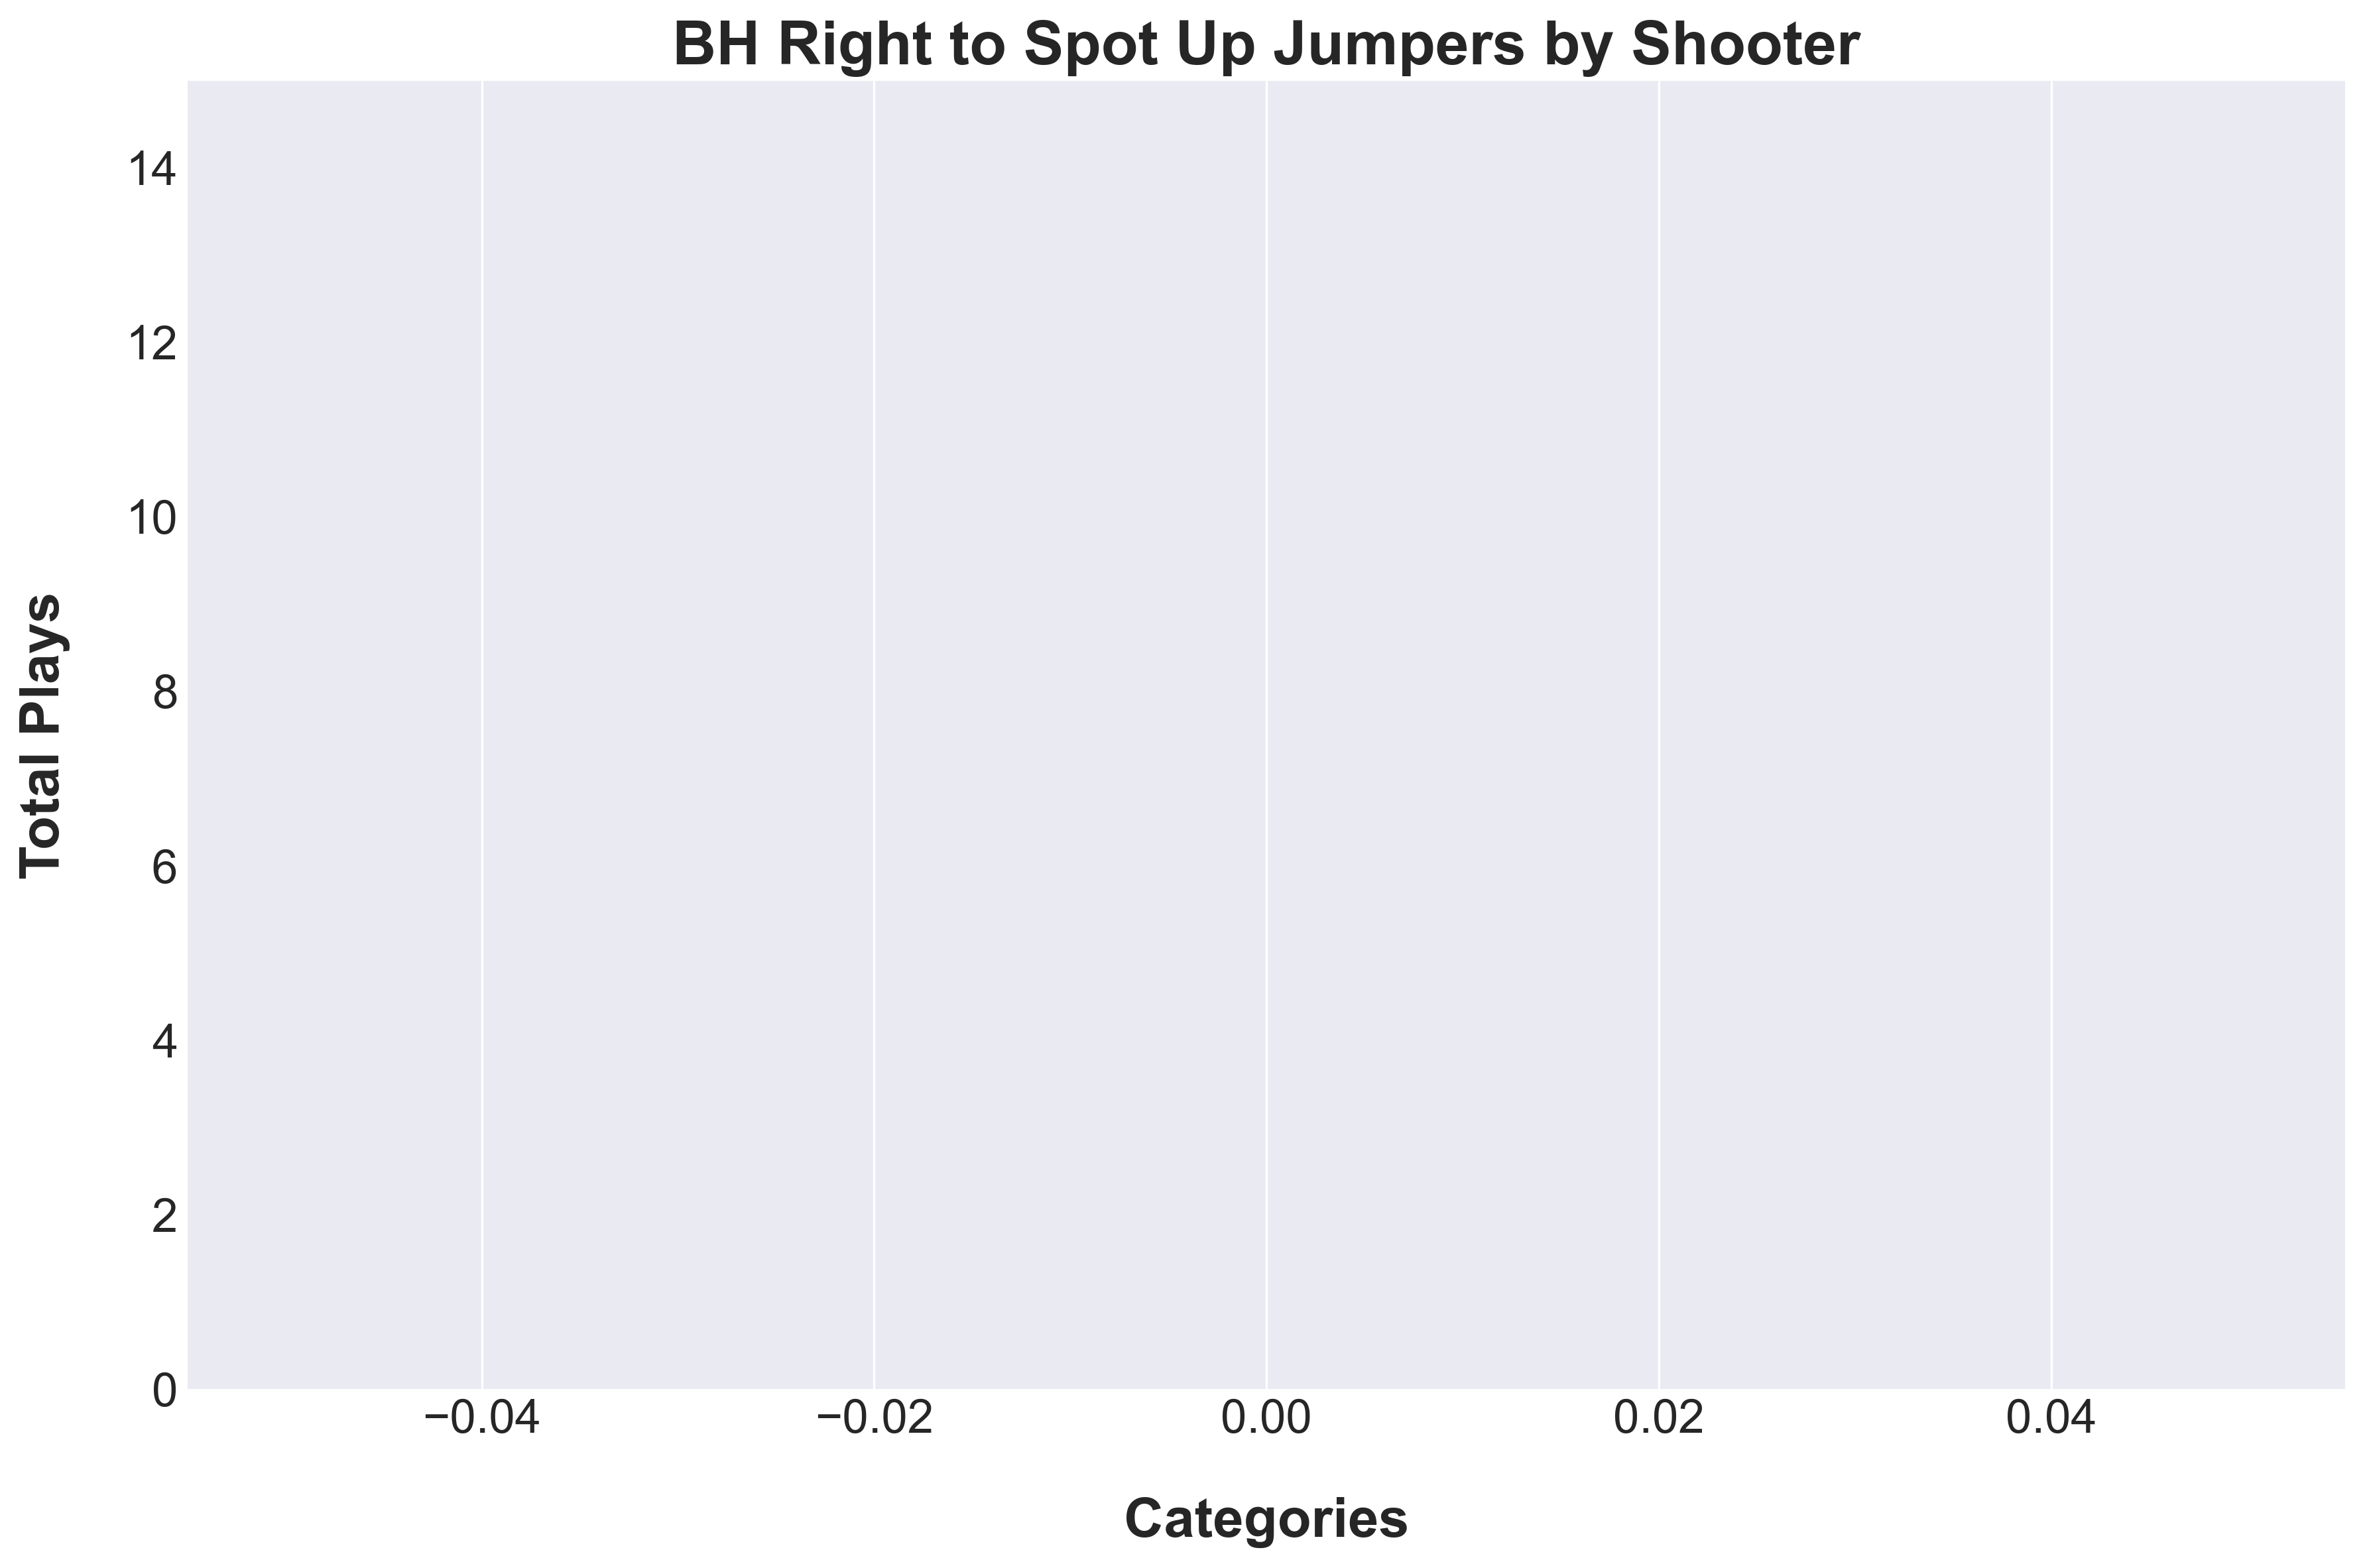
\includegraphics[width=\textwidth, height=.14\textheight]{images/PNR_PassRightShotsPlayer_Freq.png} % Adjust the width of the image to fit
    \end{minipage}
\end{table}

\vspace{-1em} % Add vertical space before the line (optional)
%\hrule height 1pt width 1\textwidth % Adjust height and width
\vspace{-1em} % Add vertical space after the line (optional)

% BH Right -> Rollman Rolls Secondary Player Stats
\begin{table}[H]
    \raisebox{3em}{ % Adjust this value to shift the tables vertically
    \begin{minipage}[t]{0.6\textwidth} % Left side (table) takes 85% of the width
        \flushleft
        \centering % Centering the title and the table
        \text{BH Right - Rollman Rolls Player Statistics} % Title above the table in bold
        \vskip .25em % Adds vertical space between title and table
        \scalebox{.6}{ % Scale the entire table down by half
            \renewcommand{\arraystretch}{1.4} % Adjust the number to increase or decrease row spacing
            \begin{tabular}{
            >{\centering\arraybackslash}p{3cm} 
            >{\centering\arraybackslash}p{.75cm} 
            >{\centering\arraybackslash}p{.75cm} 
            >{\centering\arraybackslash}p{.75cm} 
            >{\centering\arraybackslash}p{.75cm}
            >{\centering\arraybackslash}p{.75cm} 
            >{\centering\arraybackslash}p{.75cm}
            >{\centering\arraybackslash}p{.75cm}
            >{\centering\arraybackslash}p{.75cm} 
            >{\centering\arraybackslash}p{.75cm}}% Adjust column widths
            \toprule
            {\scriptsize \textbf{Player}} &
            {\scriptsize \textbf{Plays}} &
            {\scriptsize \textbf{2PA}} & 
            {\scriptsize \textbf{2PM}} & 
            {\scriptsize \textbf{2P\%}} & 
            {\scriptsize \textbf{MiA}} & 
            {\scriptsize \textbf{MiM}} &
            {\scriptsize \textbf{Mi\%}} &
            {\scriptsize \textbf{TO}} &
            {\scriptsize \textbf{Foul}} \\
            \midrule
            
                
            
                
            
                
            
                
            
                
            
                
            
                
            
                
            
                
            
                
            
                
            
                
            
                
            
                
            
                
            
                
            
                
            
                
            
                
            
                
            
                
            
                
                    
                        Kenny Wilburn & 
                        3 & 
                        3 & 
                        3 & 
                        - & 
                        0 & 
                        0 & 
                        - & 
                        0 & 
                        0 \\
                    
                
            
                
            
                
            
                
            
                
            
                
            
                
            
                
            
                
            
                
            
                
            
                
            
                
            
                
            
                
            
                
            
                
            

            \bottomrule
        \end{tabular}
        } % End of \scalebox
    \end{minipage}
    } % End of raisebox, closing the adjustment
    \hfill % This adds some flexible space between the table and the image
    \begin{minipage}[c]{0.35\textwidth} % Right side (image) takes 10% of the width
        \flushright
        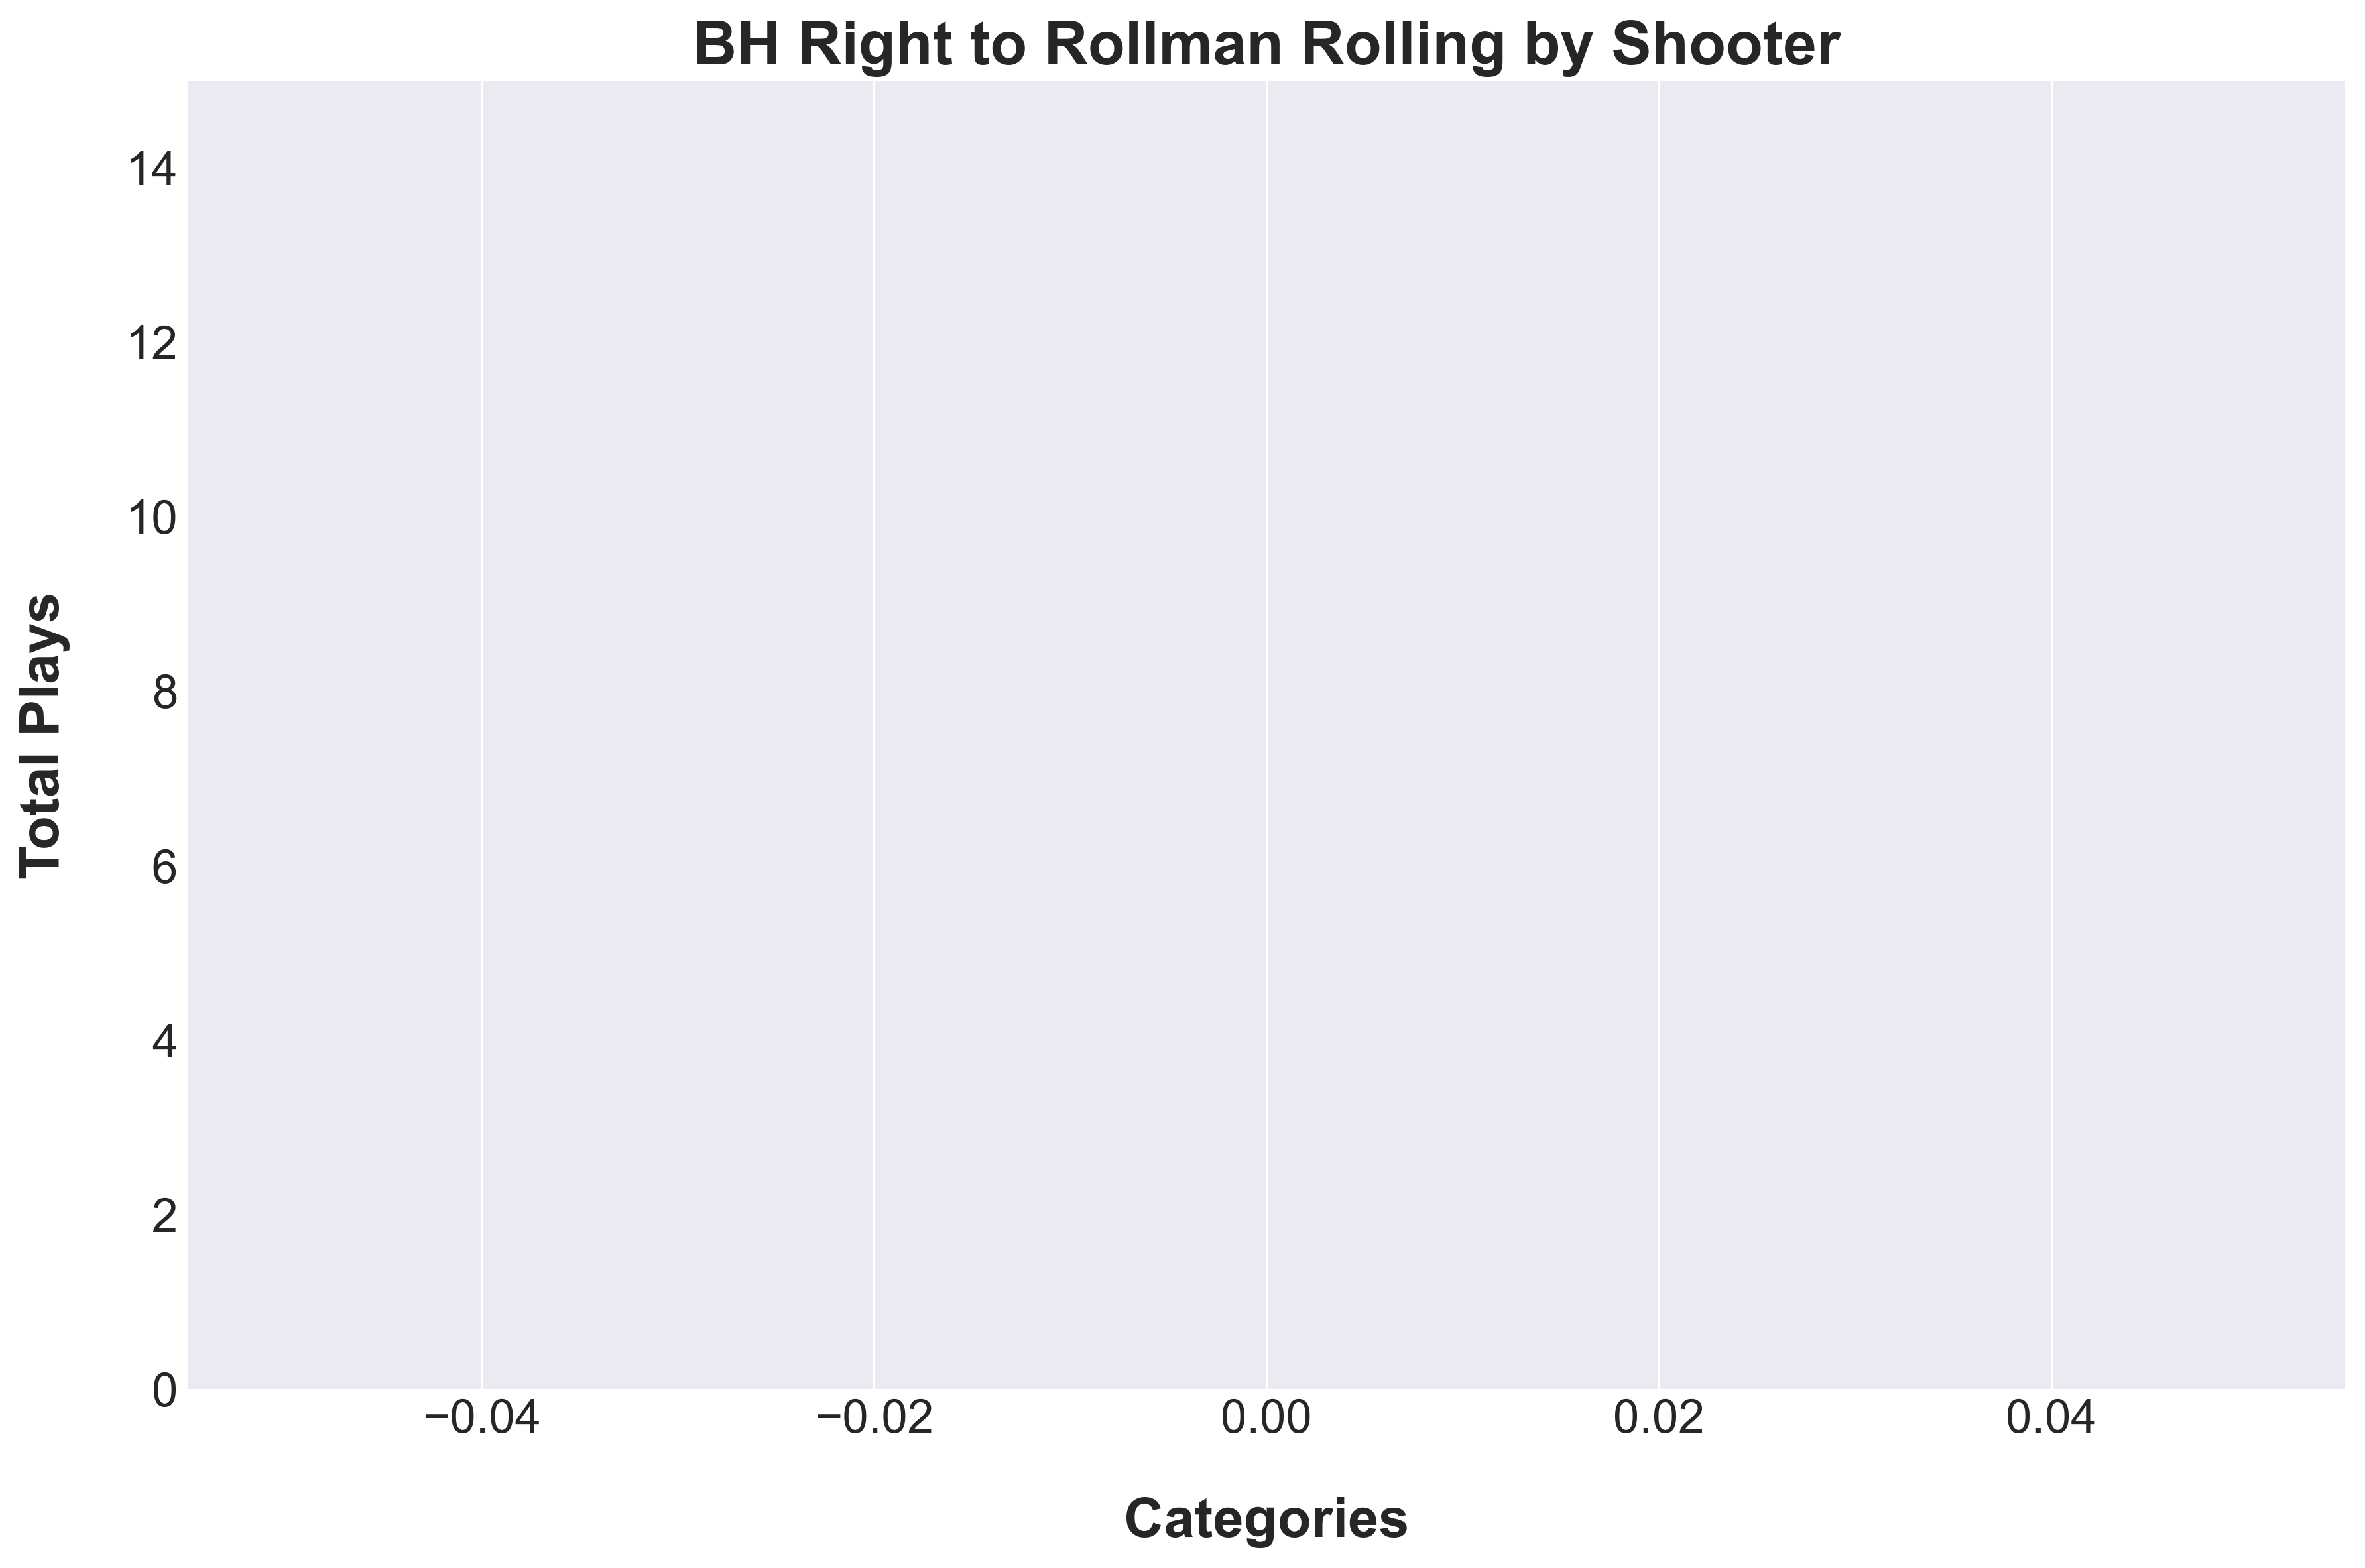
\includegraphics[width=\textwidth, height=.14\textheight]{images/PNR_PassRightRollsPlayer_Freq.png} % Adjust the width of the image to fit
    \end{minipage}
\end{table}

\vspace{-1em} % Add vertical space before the line (optional)
%\hrule height 1pt width 1\textwidth % Adjust height and width
\vspace{-1em} % Add vertical space after the line (optional)

% BH Right -> Rollman Slips Secondary Player Stats
\begin{table}[H]
    \raisebox{3em}{ % Adjust this value to shift the tables vertically
    \begin{minipage}[t]{0.6\textwidth} % Left side (table) takes 85% of the width
        \flushleft
        \centering % Centering the title and the table
        \text{BH Right - Rollman Slips Player Statistics} % Title above the table in bold
        \vskip .25em % Adds vertical space between title and table
        \scalebox{.55}{ % Scale the entire table down by half
            \renewcommand{\arraystretch}{1.4} % Adjust the number to increase or decrease row spacing
            \begin{tabular}{
            >{\centering\arraybackslash}p{3cm} 
            >{\centering\arraybackslash}p{.75cm} 
            >{\centering\arraybackslash}p{.75cm} 
            >{\centering\arraybackslash}p{.75cm} 
            >{\centering\arraybackslash}p{.75cm}
            >{\centering\arraybackslash}p{.75cm} 
            >{\centering\arraybackslash}p{.75cm} 
            >{\centering\arraybackslash}p{.75cm} 
            >{\centering\arraybackslash}p{.75cm}
            >{\centering\arraybackslash}p{.75cm} 
            >{\centering\arraybackslash}p{.75cm}
            >{\centering\arraybackslash}p{.75cm}
            >{\centering\arraybackslash}p{.75cm} 
            >{\centering\arraybackslash}p{.75cm}}% Adjust column widths
            \toprule
            {\scriptsize \textbf{Player}} &
            {\scriptsize \textbf{Plays}} &
            {\scriptsize \textbf{3PA}} &
            {\scriptsize \textbf{3PM}} &
            {\scriptsize \textbf{3P\%}} & 
            {\scriptsize \textbf{2PA}} & 
            {\scriptsize \textbf{2PM}} & 
            {\scriptsize \textbf{2P\%}} & 
            {\scriptsize \textbf{MiA}} & 
            {\scriptsize \textbf{MiM}} &
            {\scriptsize \textbf{Mi\%}} &
            {\scriptsize \textbf{EFG\%}} &
            {\scriptsize \textbf{TO}} &
            {\scriptsize \textbf{Foul}} \\
            \midrule
            
                
            
                
            
                
            
                
            
                
            
                
            
                
            
                
            
                
            
                
            
                
            
                
            
                
            
                
            
                
            
                
            
                
            
                
            
                
            
                
            
                
            
                
            
                
                    
                
            
                
            
                
            
                
            
                
            
                
            
                
            
                
            
                
            
                
            
                
            
                
            
                
            
                
            
                
            
                
            

            \bottomrule
        \end{tabular}
        } % End of \scalebox
    \end{minipage}
    } % End of raisebox, closing the adjustment
    \hfill % This adds some flexible space between the table and the image
    \begin{minipage}[c]{0.35\textwidth} % Right side (image) takes 10% of the width
        \flushright
        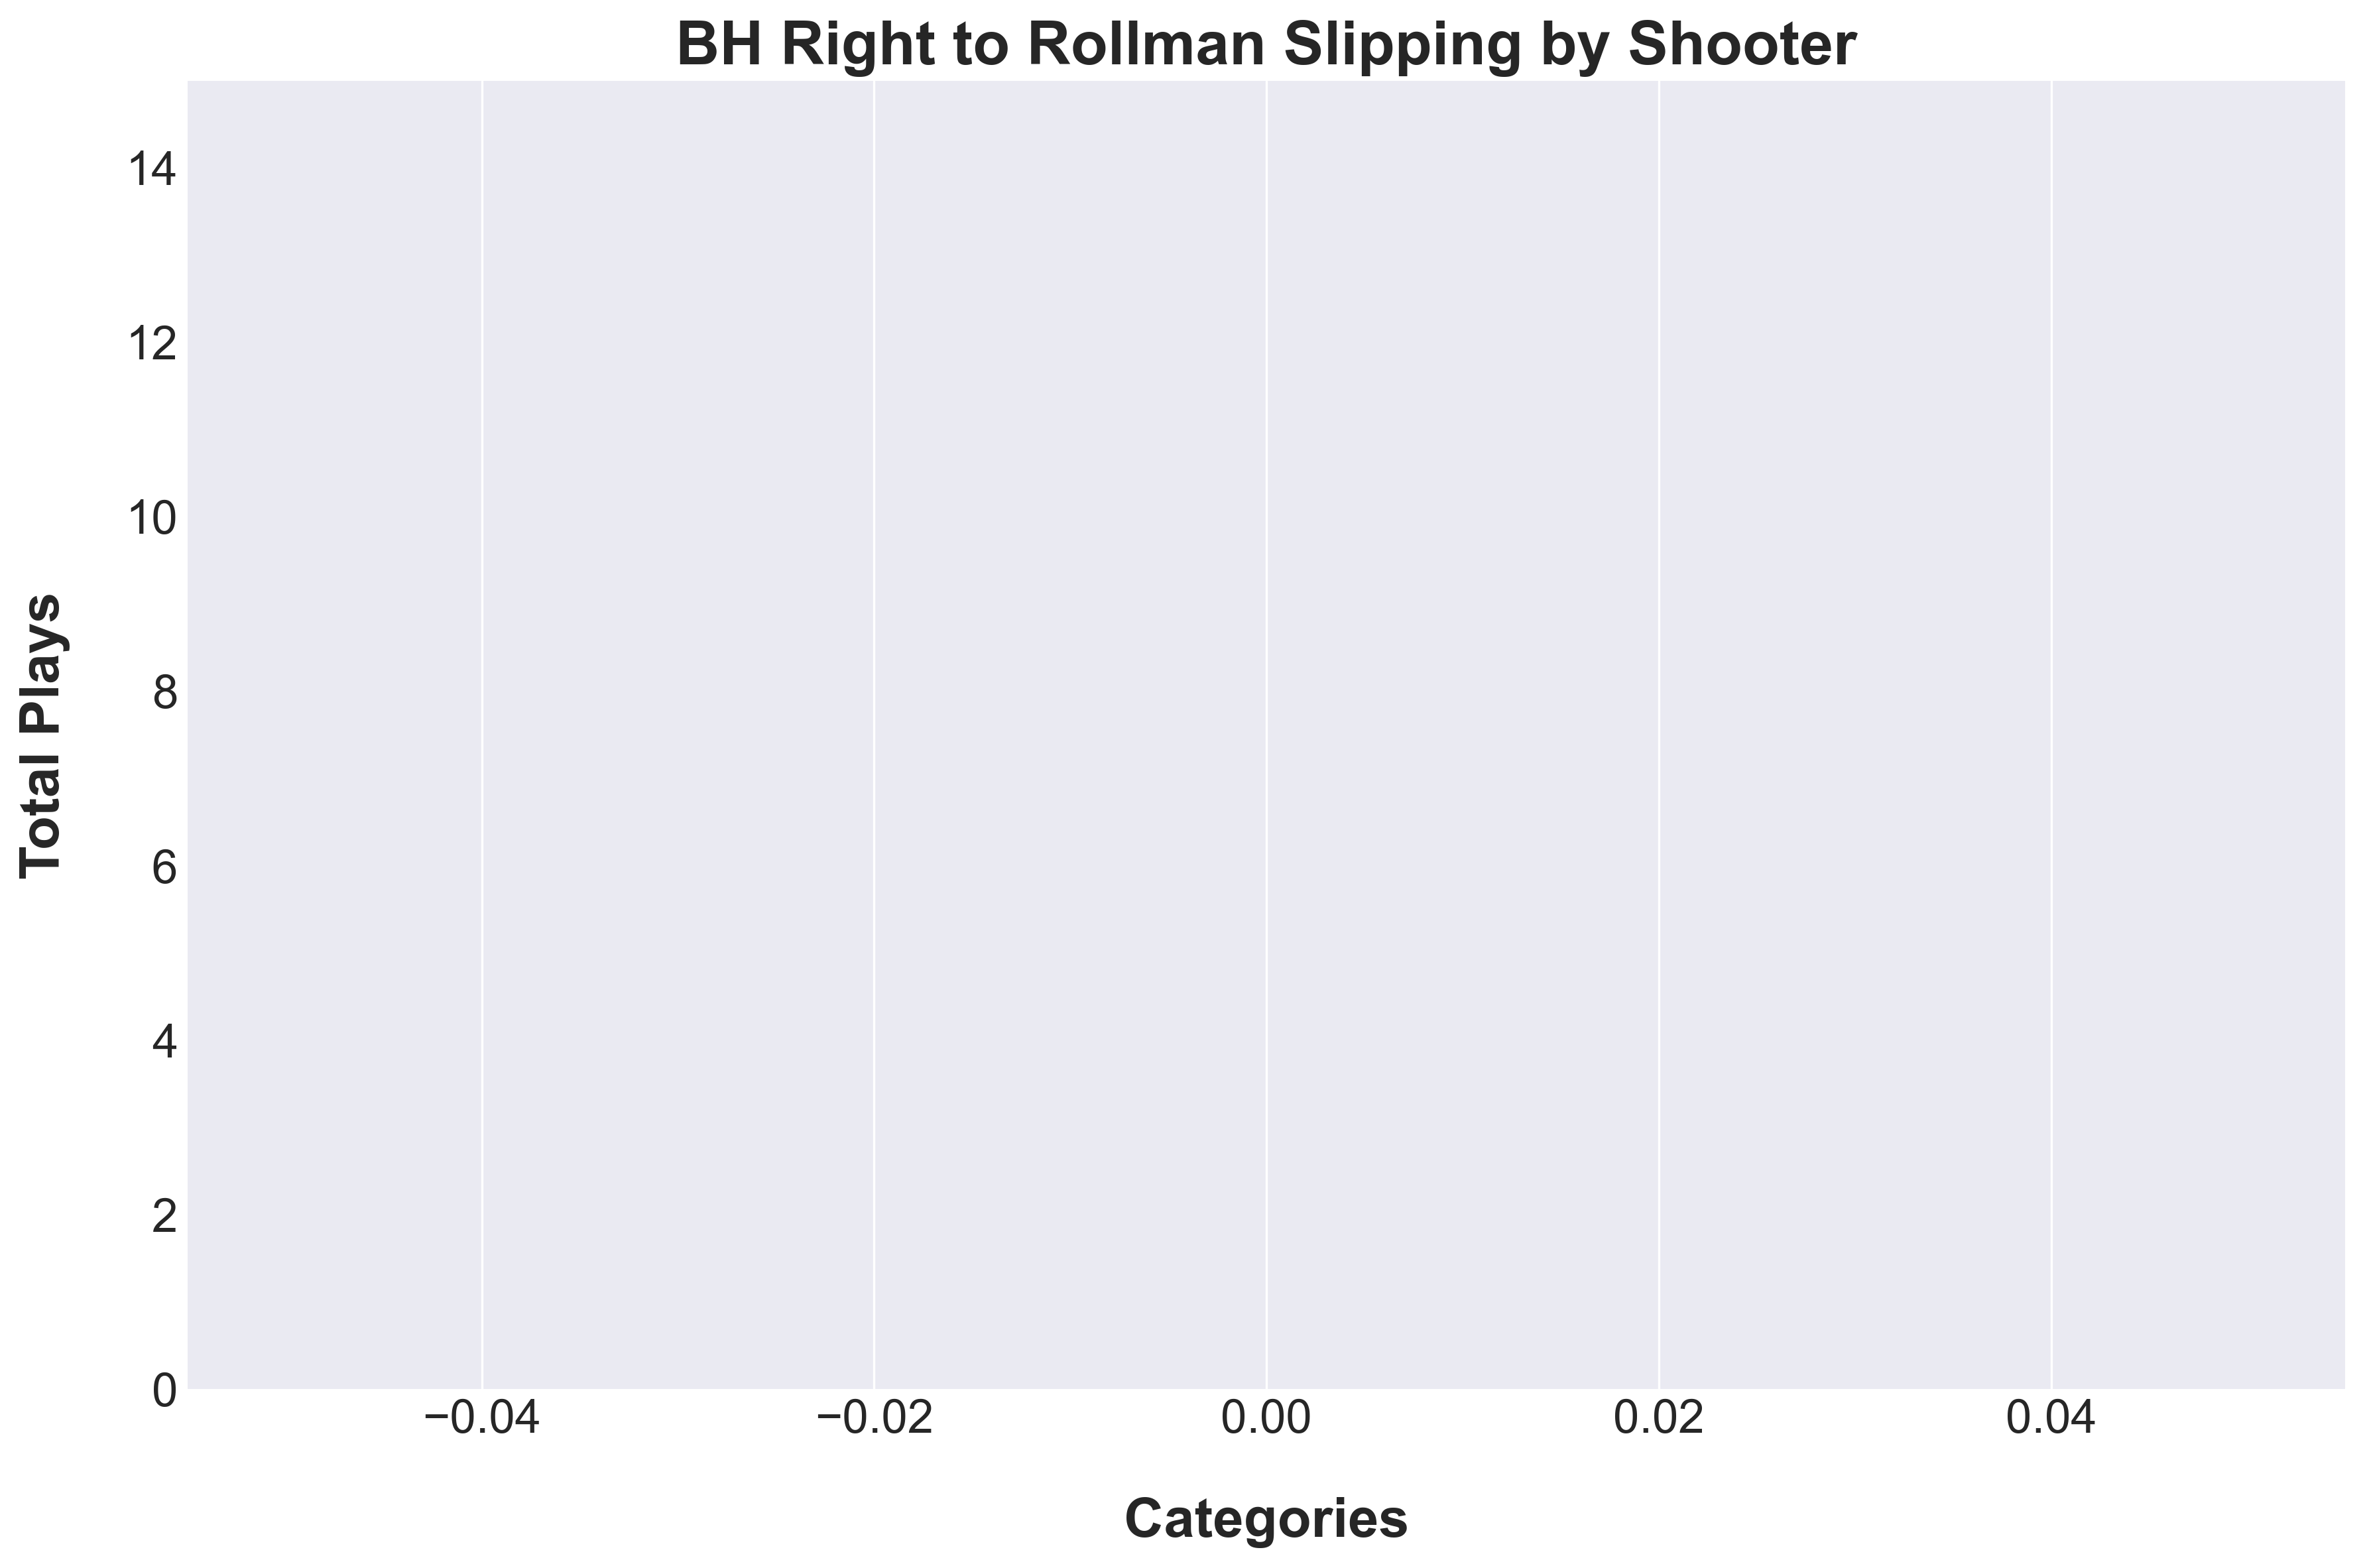
\includegraphics[width=\textwidth, height=.14\textheight]{images/PNR_PassRightSlipsPlayer_Freq.png} % Adjust the width of the image to fit
    \end{minipage}
\end{table}

\vspace{-1em} % Add vertical space before the line (optional)
%\hrule height 1pt width 1\textwidth % Adjust height and width
\vspace{-1em} % Add vertical space after the line (optional)

% BH Right -> Rollman Pops Secondary Player Stats
\begin{table}[H]
    \raisebox{3em}{ % Adjust this value to shift the tables vertically
    \begin{minipage}[t]{0.6\textwidth} % Left side (table) takes 85% of the width
        \flushleft
        \centering % Centering the title and the table
        \text{BH Right - Rollman Pops Player Statistics} % Title above the table in bold
        \vskip .25em % Adds vertical space between title and table
        \scalebox{.55}{ % Scale the entire table down by half
            \renewcommand{\arraystretch}{1.4} % Adjust the number to increase or decrease row spacing
            \begin{tabular}{
            >{\centering\arraybackslash}p{3cm} 
            >{\centering\arraybackslash}p{.75cm} 
            >{\centering\arraybackslash}p{.75cm} 
            >{\centering\arraybackslash}p{.75cm} 
            >{\centering\arraybackslash}p{.75cm}
            >{\centering\arraybackslash}p{.75cm} 
            >{\centering\arraybackslash}p{.75cm} 
            >{\centering\arraybackslash}p{.75cm} 
            >{\centering\arraybackslash}p{.75cm}
            >{\centering\arraybackslash}p{.75cm} 
            >{\centering\arraybackslash}p{.75cm}
            >{\centering\arraybackslash}p{.75cm}
            >{\centering\arraybackslash}p{.75cm} 
            >{\centering\arraybackslash}p{.75cm}}% Adjust column widths
            \toprule
            {\scriptsize \textbf{Player}} &
            {\scriptsize \textbf{Plays}} &
            {\scriptsize \textbf{3PA}} &
            {\scriptsize \textbf{3PM}} &
            {\scriptsize \textbf{3P\%}} & 
            {\scriptsize \textbf{2PA}} & 
            {\scriptsize \textbf{2PM}} & 
            {\scriptsize \textbf{2P\%}} & 
            {\scriptsize \textbf{MiA}} & 
            {\scriptsize \textbf{MiM}} &
            {\scriptsize \textbf{Mi\%}} &
            {\scriptsize \textbf{EFG\%}} &
            {\scriptsize \textbf{TO}} &
            {\scriptsize \textbf{Foul}} \\
            \midrule
            
                
            
                
            
                
            
                
            
                
            
                
            
                
            
                
            
                
            
                
            
                
            
                
            
                
            
                
            
                
            
                
            
                
            
                
            
                
            
                
            
                
            
                
            
                
            
                
                    
                        Josiah Turner & 
                        2 & 
                        0 & 
                        0 & 
                        - & 
                        1 & 
                        1 & 
                        - & 
                        1 & 
                        1 & 
                        - & 
                        - & 
                        0 & 
                        1 \\
                    
                        Kenny Wilburn & 
                        1 & 
                        0 & 
                        0 & 
                        - & 
                        1 & 
                        0 & 
                        - & 
                        0 & 
                        0 & 
                        - & 
                        - & 
                        0 & 
                        0 \\
                    
                
            
                
            
                
            
                
            
                
            
                
            
                
            
                
            
                
            
                
            
                
            
                
            
                
            
                
            
                
            

            \bottomrule
        \end{tabular}
        } % End of \scalebox
    \end{minipage}
    } % End of raisebox, closing the adjustment
    \hfill % This adds some flexible space between the table and the image
    \begin{minipage}[c]{0.35\textwidth} % Right side (image) takes 10% of the width
        \flushright
        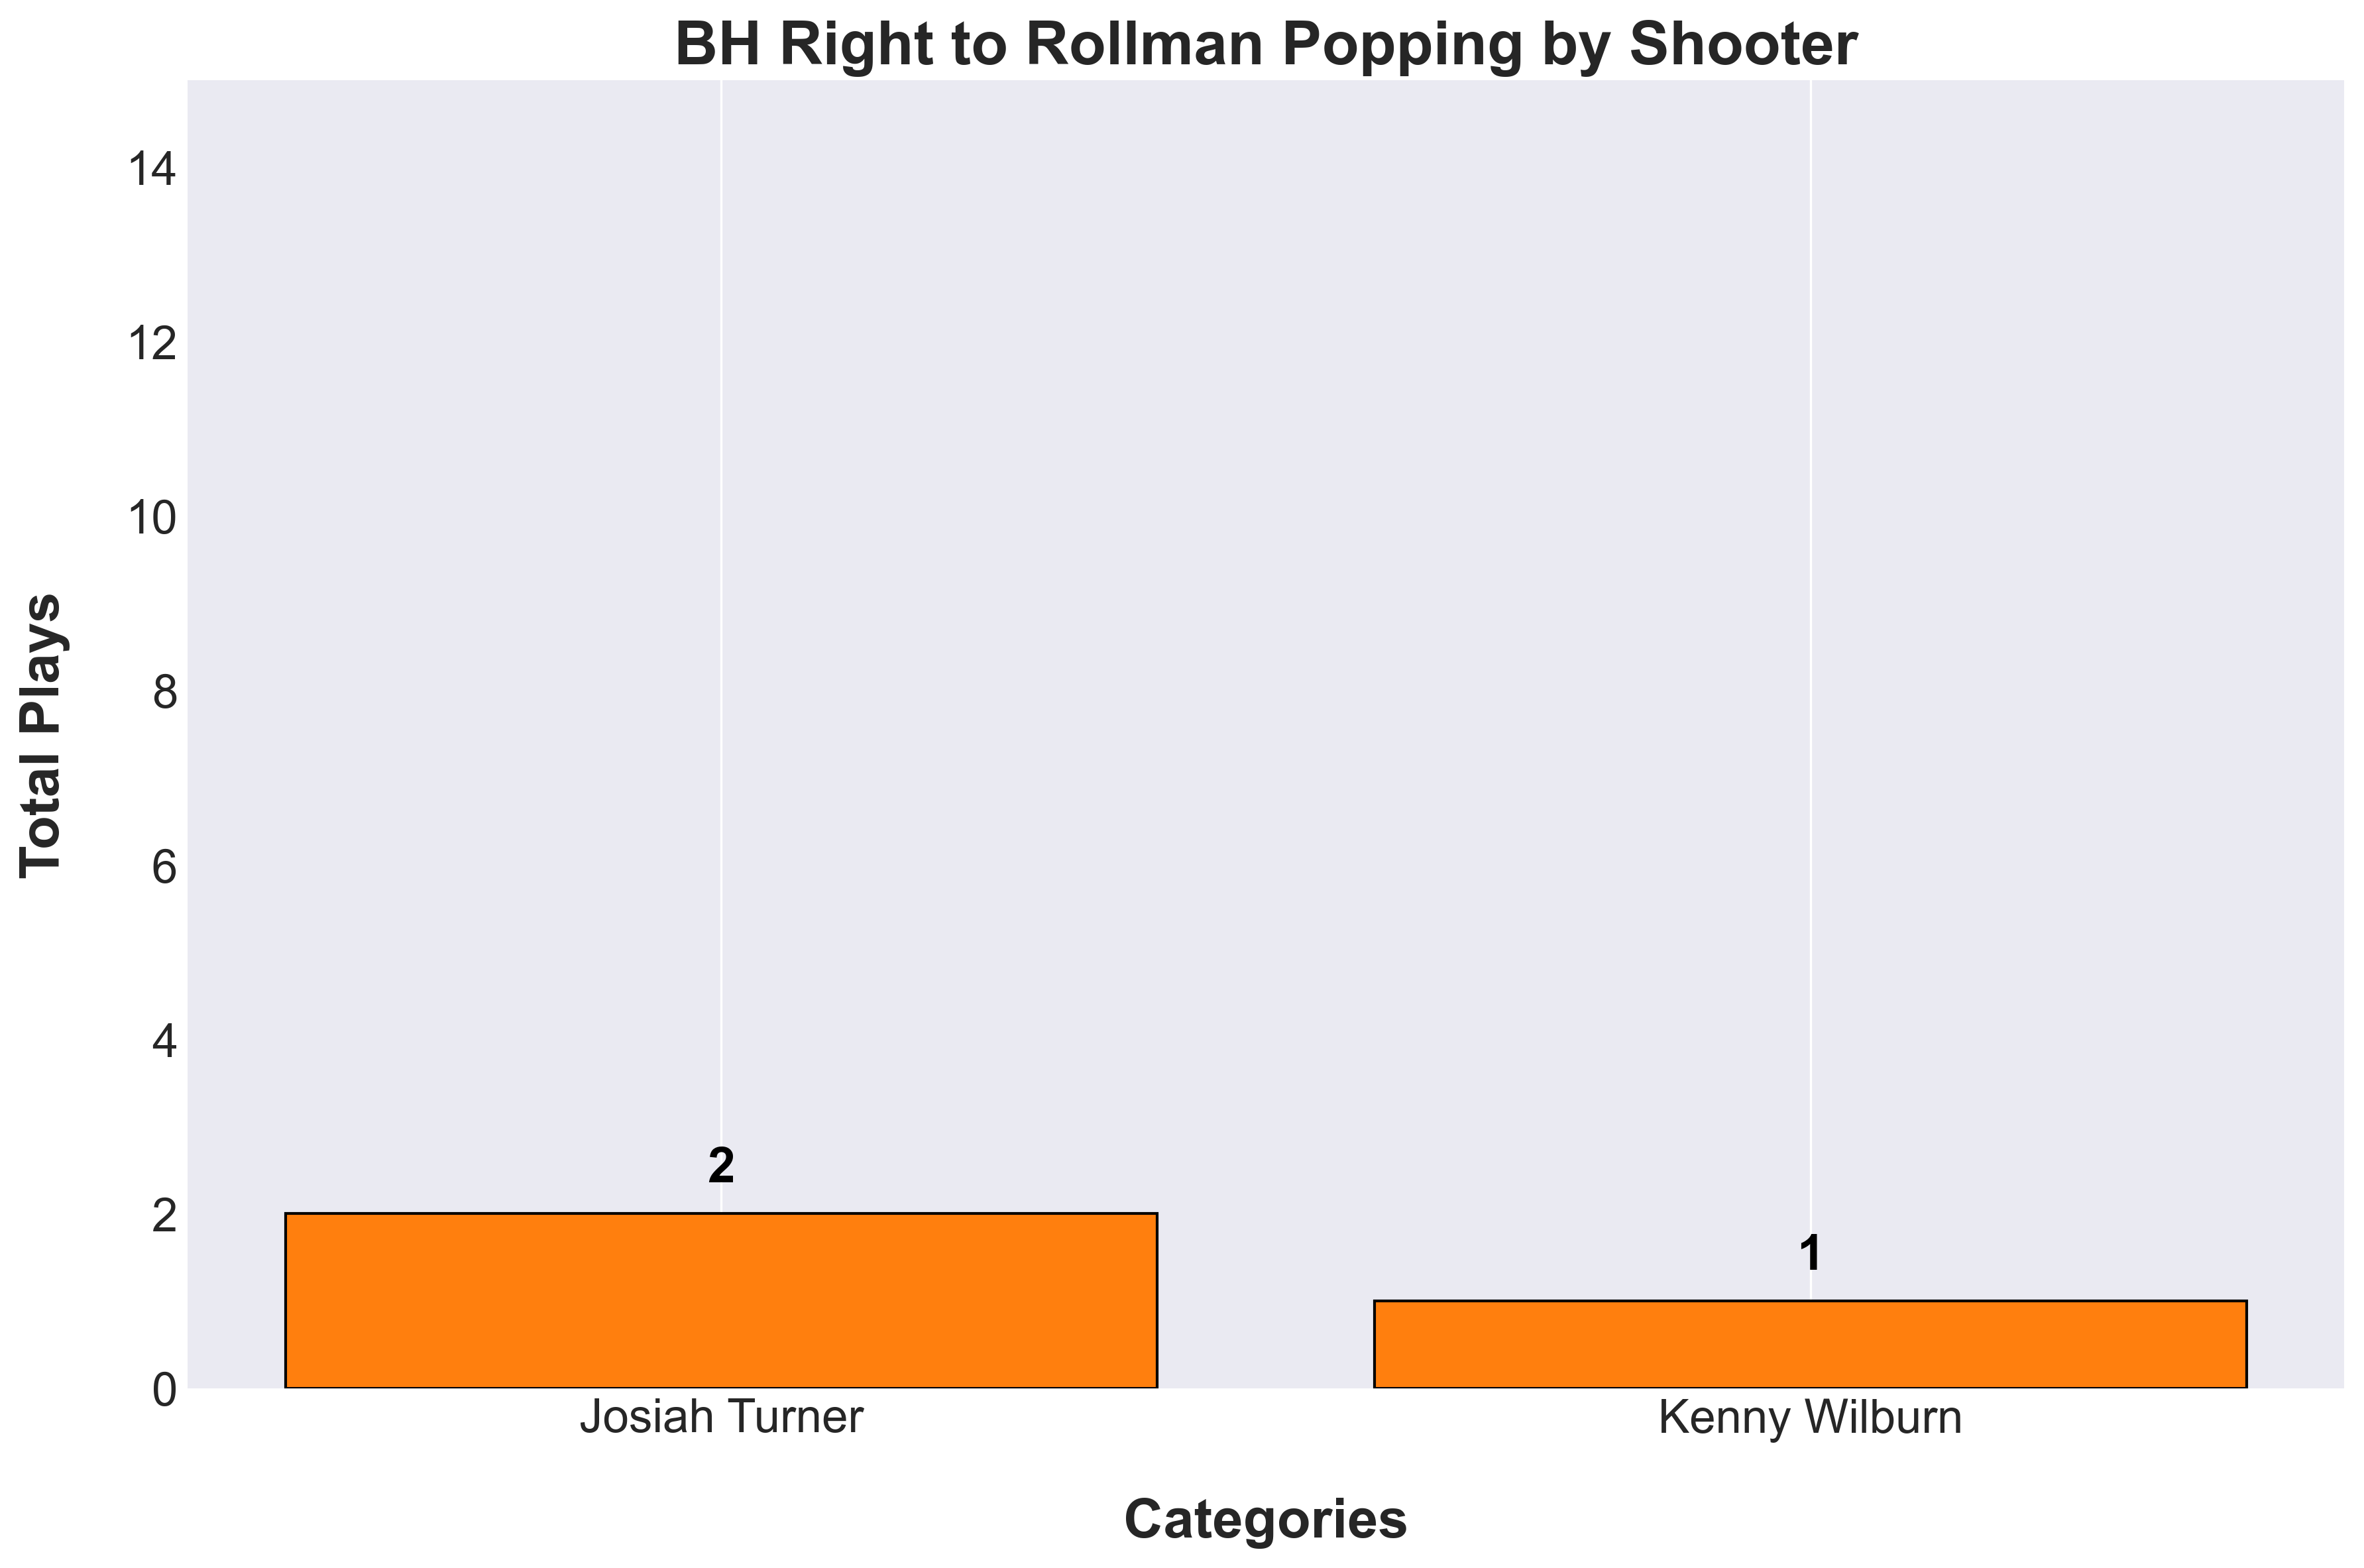
\includegraphics[width=\textwidth, height=.14\textheight]{images/PNR_PassRightPopsPlayer_Freq.png} % Adjust the width of the image to fit
    \end{minipage}
\end{table}

\vspace{-1em} % Add vertical space before the line (optional)
\hrule height 1pt width 1\textwidth % Adjust height and width
\vspace{1em} % Add vertical space after the line (optional)

\clearpage

% ----------------------
% Post Ups Visuals and Insights Section
% ----------------------
\subsection{Post-Ups}

\vspace{1.25em} % Add vertical space before the line (optional)
\textbf{Key Notes on Post Up Tendencies}
\vspace{0.5em} % Add space between the title and the itemized list

\begin{itemize}
    \item Post Ups make up x\% of players offensive load
    \vspace{0.3em} % Add space between the title and the itemized list
    \item Player is more efficient shooting over his left shoulder and get shots off of the left block x\% of the time which is much higher than the middle and right block.
\end{itemize}

\vspace{1em} % Add vertical space before the line (optional)
\hrule height 1pt width 1\textwidth % Adjust height and width
\vspace{0em} % Add vertical space after the line (optional)

\subsubsection{Post Shot Statistics}

% All Post Up Statistics Table w/ room for insights
\begin{table}[H]
    \centering
    \begin{minipage}[t]{0.6\textwidth} % Left side (table) takes 85% of the width
        %\flushright
        \centering % Centering the title and the table
        \text{Total Post Shot Statistics} % Title above the table in bold
        \vskip .25em % Adds vertical space between title and table
        \scalebox{.85}{ % Scale the entire table down by half
            \scriptsize % Reduce the font size
            \begin{tabular}{
            >{\centering\arraybackslash}p{.75cm} 
            >{\centering\arraybackslash}p{.5cm} 
            >{\centering\arraybackslash}p{.5cm} 
            >{\centering\arraybackslash}p{.5cm}
            >{\centering\arraybackslash}p{.5cm} 
            >{\centering\arraybackslash}p{.5cm} 
            >{\centering\arraybackslash}p{.5cm}
            >{\centering\arraybackslash}p{.5cm} 
            >{\centering\arraybackslash}p{.5cm}}% Adjust column widths
            \toprule
            \textbf{Plays} &
            \textbf{2PA} & 
            \textbf{2PM} & 
            \textbf{2P\%} & 
            \textbf{MiA} & 
            \textbf{MiM} &
            \textbf{Mi\%} &
            \textbf{TO} &
            \textbf{Foul} \\
            \midrule
            
                
            
                
            
                
            
                
            
                
            
                
                    2 &
                    1 & 1 &
                    - &
                    0 & 0 &
                    - &
                    0 & 1 \\
                
            
                
            
                
            
                
            
                
            
                
            
                
            
                
            
                
            
                
            
                
            
                
            
                
            
                
            
                
            
                
            
                
            
                
            


            \bottomrule
            \end{tabular}
        }
    \end{minipage}
\end{table}

\vspace{0em} % Add vertical space before the line (optional)
%\hrule height 1pt width 1\textwidth % Adjust height and width
\vspace{-1em} % Add vertical space after the line (optional)

% Post Stats of where player shoots from Middle vs Left Block vs Right Block
\begin{table}[H]
    \raisebox{3em}{ % Adjust this value to shift the tables vertically
    \begin{minipage}[t]{0.6\textwidth} % Left side (table) takes 85% of the width
        \flushleft
        \centering % Centering the title and the table
        \text{Post Up Location Statistics} % Title above the table in bold
        \vskip .25em % Adds vertical space between title and table
        \scalebox{.6}{ % Scale the entire table down by half
            \renewcommand{\arraystretch}{1.4} % Adjust the number to increase or decrease row spacing
            \begin{tabular}{
            >{\centering\arraybackslash}p{2.5cm} 
            >{\centering\arraybackslash}p{.75cm} 
            >{\centering\arraybackslash}p{.75cm} 
            >{\centering\arraybackslash}p{.75cm} 
            >{\centering\arraybackslash}p{.75cm}
            >{\centering\arraybackslash}p{.75cm} 
            >{\centering\arraybackslash}p{.75cm}
            >{\centering\arraybackslash}p{.75cm}
            >{\centering\arraybackslash}p{.75cm} 
            >{\centering\arraybackslash}p{.75cm}}% Adjust column widths
            \toprule
            {\scriptsize \textbf{Location}} &
            {\scriptsize \textbf{Plays}} &
            {\scriptsize \textbf{2PA}} & 
            {\scriptsize \textbf{2PM}} & 
            {\scriptsize \textbf{2P\%}} & 
            {\scriptsize \textbf{MiA}} & 
            {\scriptsize \textbf{MiM}} &
            {\scriptsize \textbf{Mi\%}} &
            {\scriptsize \textbf{TO}} &
            {\scriptsize \textbf{Foul}} \\
            \midrule
            
                
            
                
            
                
            
                
            
                
            
                
            
                
            
                
                    Left Block & 2 &
                    1 & 1 &
                    - &
                    0 & 0 &
                    - &
                    0 & 1 \\
                
            
                
            
                
            
                
            
                
            
                
            
                
            
                
            
                
            
                
            
                
            
                
            
                
            
                
            
                
            
                
            


            \bottomrule
        \end{tabular}
        } % End of \scalebox
    \end{minipage}
    } % End of raisebox, closing the adjustment
    \hfill % This adds some flexible space between the table and the image
    \begin{minipage}[c]{0.35\textwidth} % Right side (image) takes 10% of the width
        \flushright
        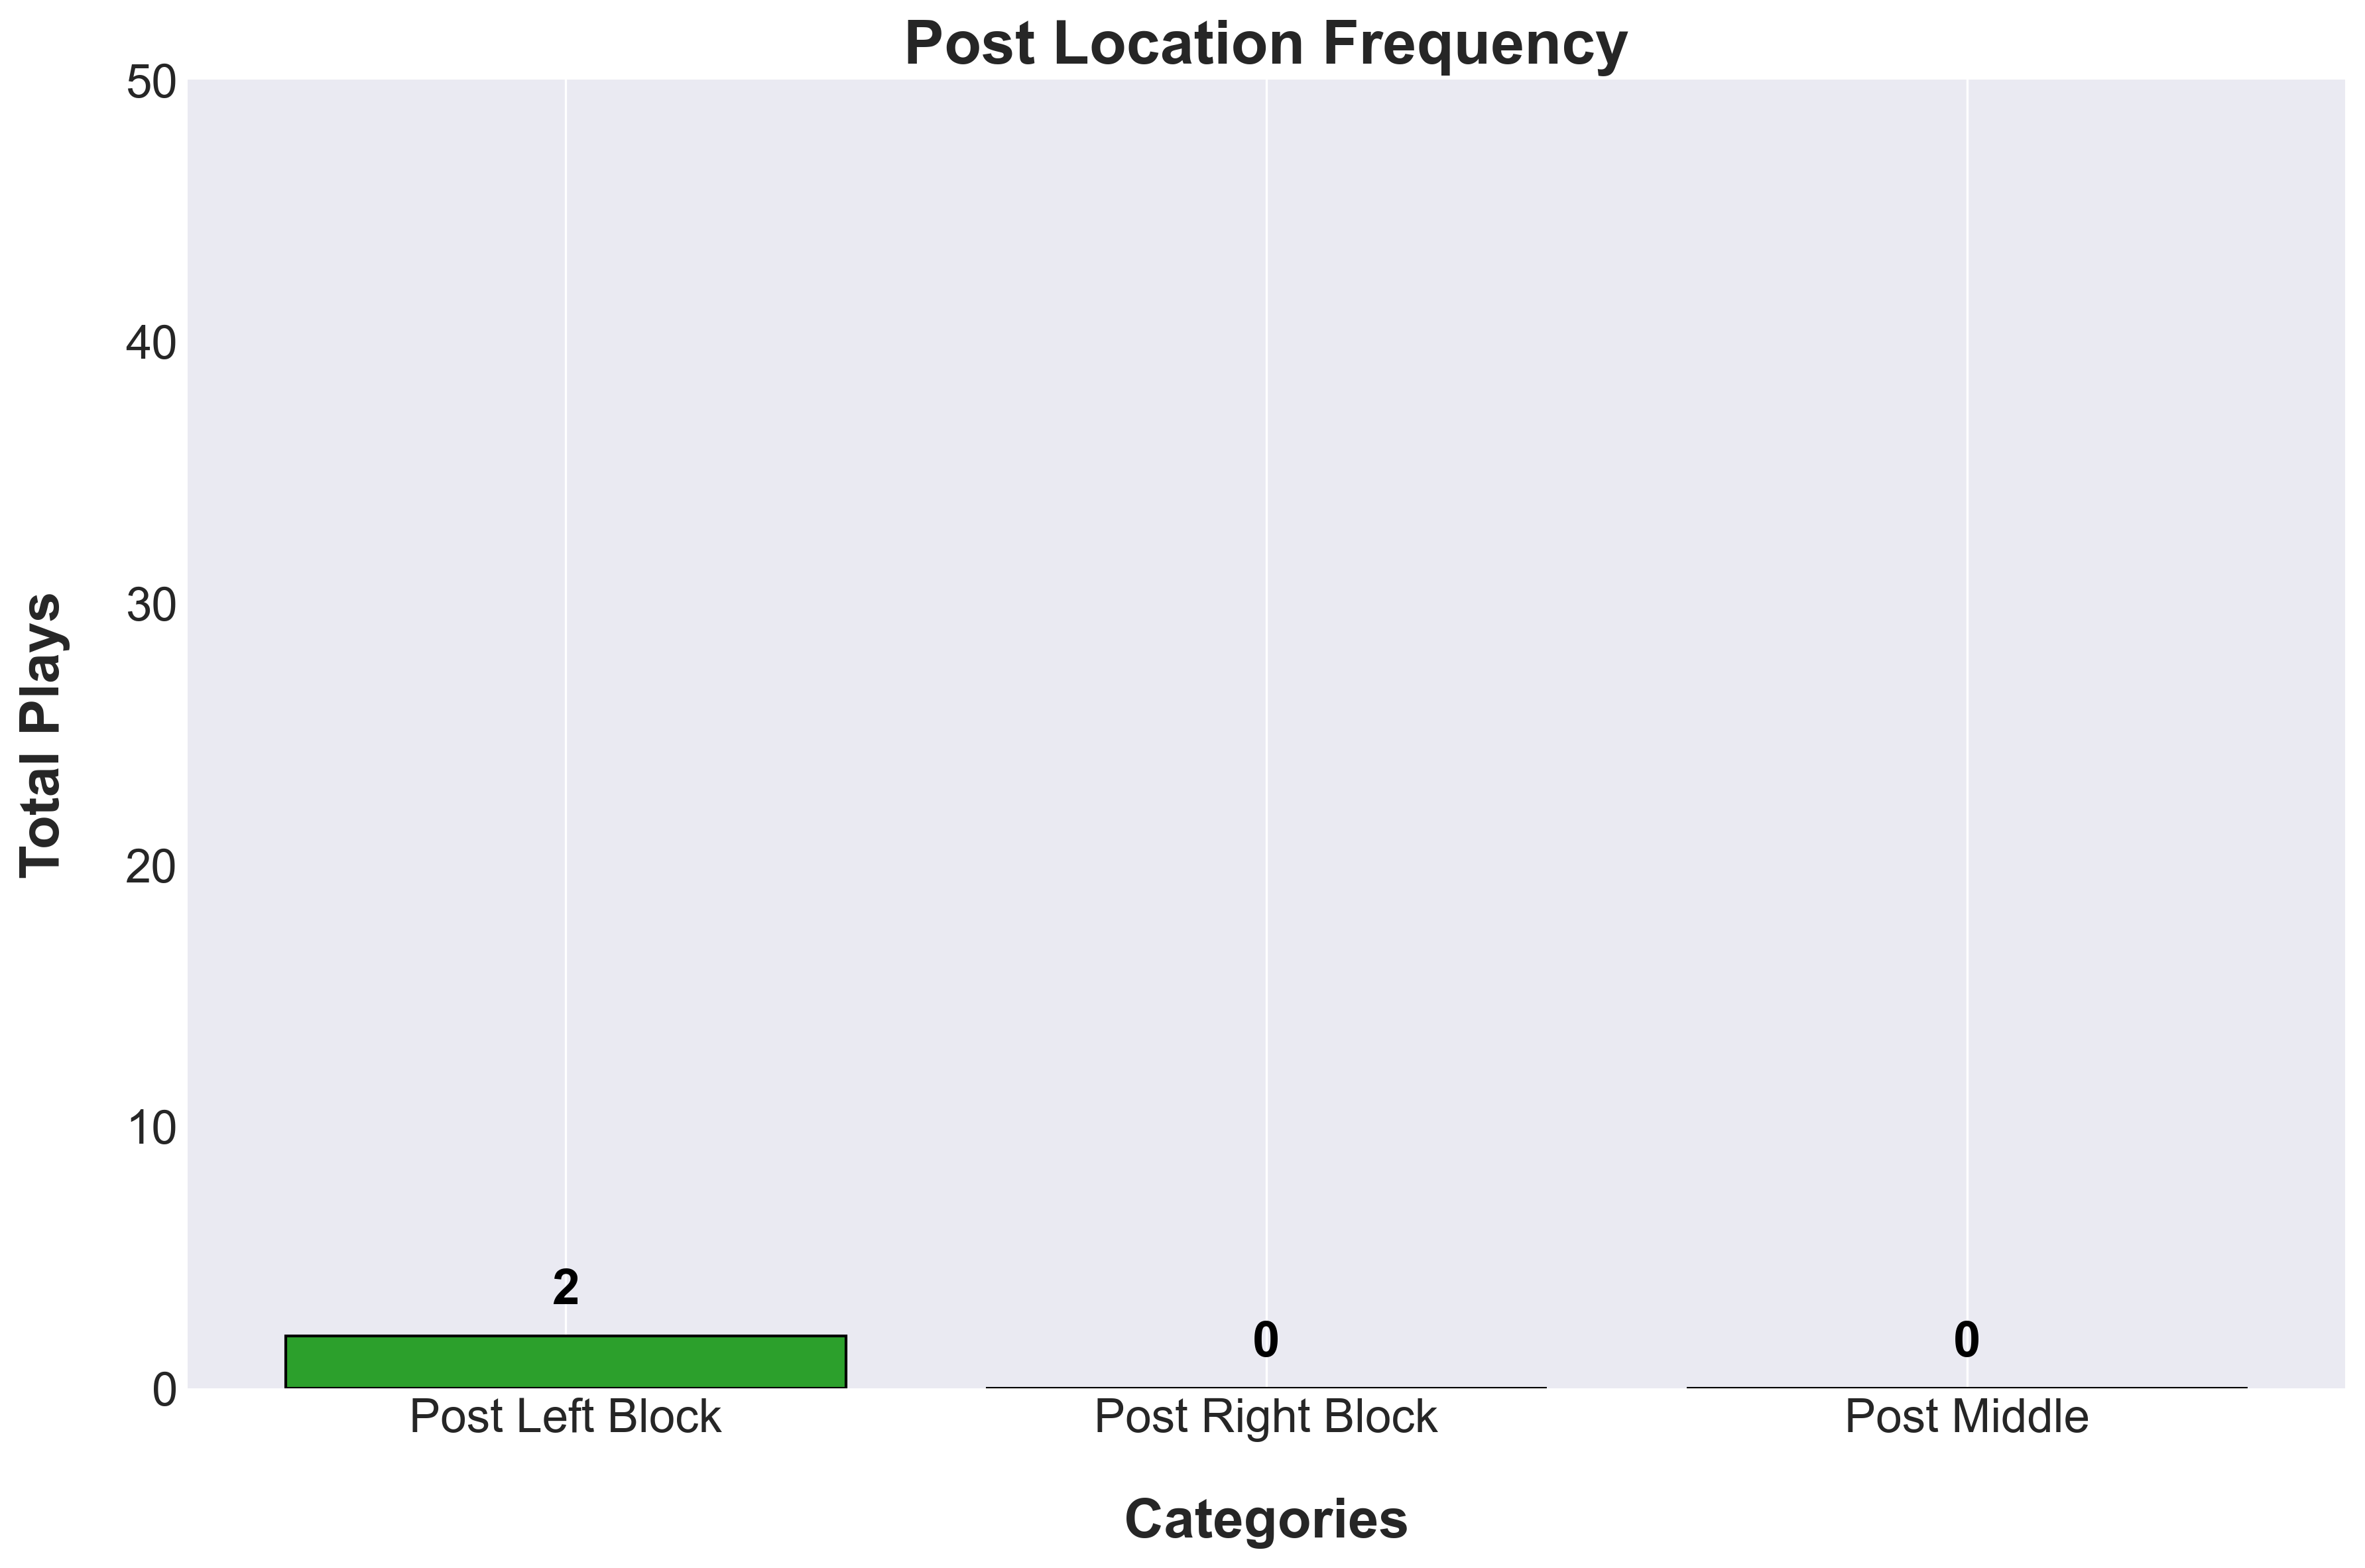
\includegraphics[width=\textwidth, height=.14\textheight]{images/Post_Location_Freq.png} % Adjust the width of the image to fit
    \end{minipage}
\end{table}

\vspace{-1em} % Add vertical space before the line (optional)
%\hrule height 1pt width 1\textwidth % Adjust height and width
\vspace{-1em} % Add vertical space after the line (optional)

% Post Shot Type Statistics
\begin{table}[H]
    \raisebox{3.5em}{ % Adjust this value to shift the tables vertically
    \begin{minipage}[t]{0.6\textwidth} % Left side (table) takes 85% of the width
        \flushleft
        \centering % Centering the title and the table
        \text{Post Shot Type Statistics} % Title above the table in bold
        \vskip .25em % Adds vertical space between title and table
        \scalebox{.6}{ % Scale the entire table down by half
            \renewcommand{\arraystretch}{1.4} % Adjust the number to increase or decrease row spacing
            \begin{tabular}{
            >{\centering\arraybackslash}p{2.75cm} 
            >{\centering\arraybackslash}p{.75cm} 
            >{\centering\arraybackslash}p{.75cm} 
            >{\centering\arraybackslash}p{.75cm} 
            >{\centering\arraybackslash}p{.75cm}
            >{\centering\arraybackslash}p{.75cm} 
            >{\centering\arraybackslash}p{.75cm}
            >{\centering\arraybackslash}p{.75cm}
            >{\centering\arraybackslash}p{.75cm} 
            >{\centering\arraybackslash}p{.75cm}}% Adjust column widths
            \toprule
            {\scriptsize \textbf{Shot Type}} &
            {\scriptsize \textbf{Plays}} &
            {\scriptsize \textbf{2PA}} & 
            {\scriptsize \textbf{2PM}} & 
            {\scriptsize \textbf{2P\%}} & 
            {\scriptsize \textbf{MiA}} & 
            {\scriptsize \textbf{MiM}} &
            {\scriptsize \textbf{Mi\%}} &
            {\scriptsize \textbf{TO}} &
            {\scriptsize \textbf{Foul}} \\
            \midrule
            
                
            
                
            
                
            
                
            
                
            
                
            
                
            
                
            
                
            
                
            
                
            
                
                    Left Shoulder & 1 &
                    0 & 0 &
                    - &
                    0 & 0 &
                    - &
                    0 & 1 \\
                
            
                
                    Right Shoulder & 1 &
                    1 & 1 &
                    - &
                    0 & 0 &
                    - &
                    0 & 0 \\
                
            
                
            
                
            
                
            
                
            
                
            
                
            
                
            
                
            
                
            
                
            


            \bottomrule
        \end{tabular}
        } % End of \scalebox
    \end{minipage}
    } % End of raisebox, closing the adjustment
    \hfill
    \begin{minipage}[c]{0.35\textwidth} % Right side (image) takes 10% of the width
        \flushright
        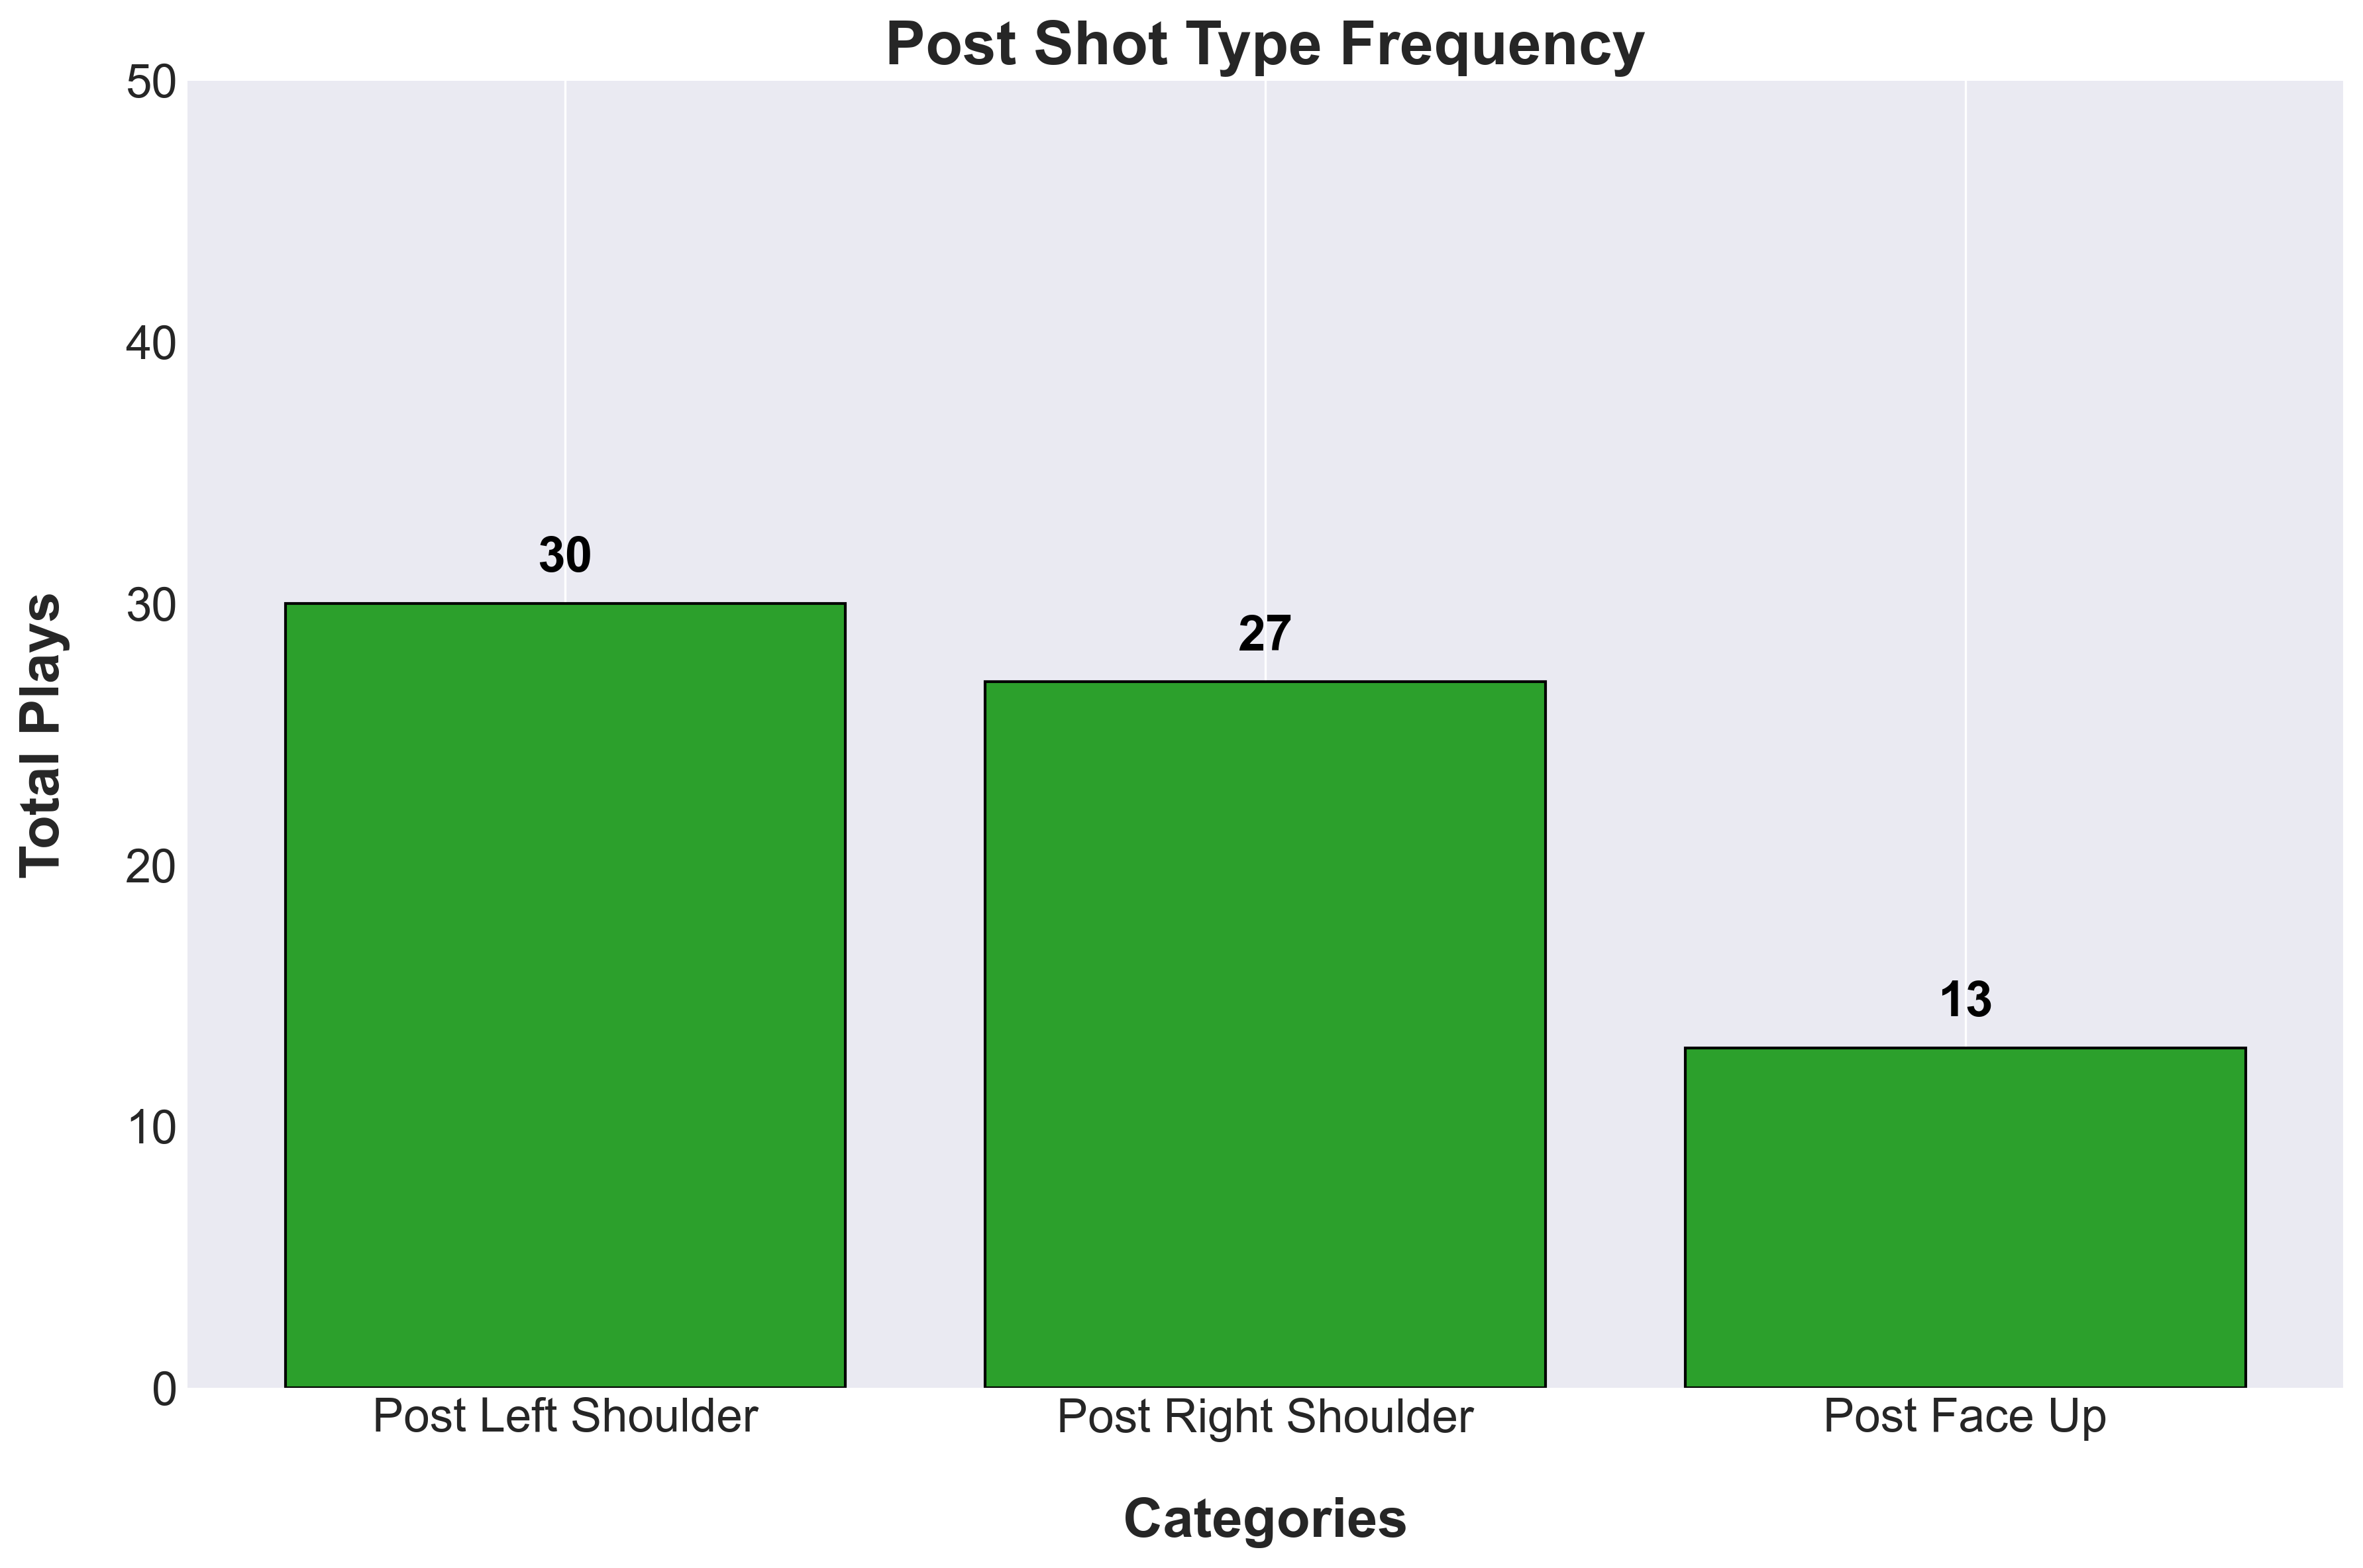
\includegraphics[width=\textwidth, height=.14\textheight]{images/Post_ShotType_Freq.png} % Adjust the width of the image to fit
    \end{minipage}
    
\end{table}

\vspace{-1em} % Add vertical space before the line (optional)
%\hrule height 1pt width 1\textwidth % Adjust height and width
\vspace{-1em} % Add vertical space after the line (optional)

% Post Stats for Combination of Location and Shot Type Stats
\begin{table}[H]
    \raisebox{6em}{ % Adjust this value to shift the tables vertically
    \begin{minipage}[t]{0.6\textwidth} % Left side (table) takes 85% of the width
        \flushleft
        \centering % Centering the title and the table
        \text{Post Combination Statistics} % Title above the table in bold
        \vskip .25em % Adds vertical space between title and table
        \scalebox{.6}{ % Scale the entire table down by half
            \renewcommand{\arraystretch}{1.4} % Adjust the number to increase or decrease row spacing
            \begin{tabular}{
            >{\centering\arraybackslash}p{5.5cm} 
            >{\centering\arraybackslash}p{.75cm} 
            >{\centering\arraybackslash}p{.75cm} 
            >{\centering\arraybackslash}p{.75cm} 
            >{\centering\arraybackslash}p{.75cm}
            >{\centering\arraybackslash}p{.75cm} 
            >{\centering\arraybackslash}p{.75cm} 
            >{\centering\arraybackslash}p{.75cm}
            >{\centering\arraybackslash}p{.75cm} 
            >{\centering\arraybackslash}p{.75cm}}% Adjust column widths
            \toprule
            {\scriptsize \textbf{PlayType}} &
            {\scriptsize \textbf{Plays}} &
            {\scriptsize \textbf{2PA}} & 
            {\scriptsize \textbf{2PM}} & 
            {\scriptsize \textbf{2P\%}} & 
            {\scriptsize \textbf{MiA}} & 
            {\scriptsize \textbf{MiM}} &
            {\scriptsize \textbf{Mi\%}} &
            {\scriptsize \textbf{TO}} &
            {\scriptsize \textbf{Foul}} \\
            \midrule
            
                
            
                
            
                
            
                
            
                
            
                
            
                
            
                
            
                
            
                
            
                
            
                
            
                
            
                
            
                
            
                
                    Left Block - Left Shoulder & 1 &
                    0 & 0 &
                    - &
                    0 & 0 &
                    - &
                    0 & 1 \\
                
            
                
                    Left Block - Right Shoulder & 1 &
                    1 & 1 &
                    - &
                    0 & 0 &
                    - &
                    0 & 0 \\
                
            
                
            
                
            
                
            
                
            
                
            
                
            


            \bottomrule
        \end{tabular}
        } % End of \scalebox
    \end{minipage}
    } % End of raisebox, closing the adjustment
    \hfill % This adds some flexible space between the table and the image
    \begin{minipage}[c]{0.35\textwidth} % Right side (image) takes 10% of the width
        \flushright
        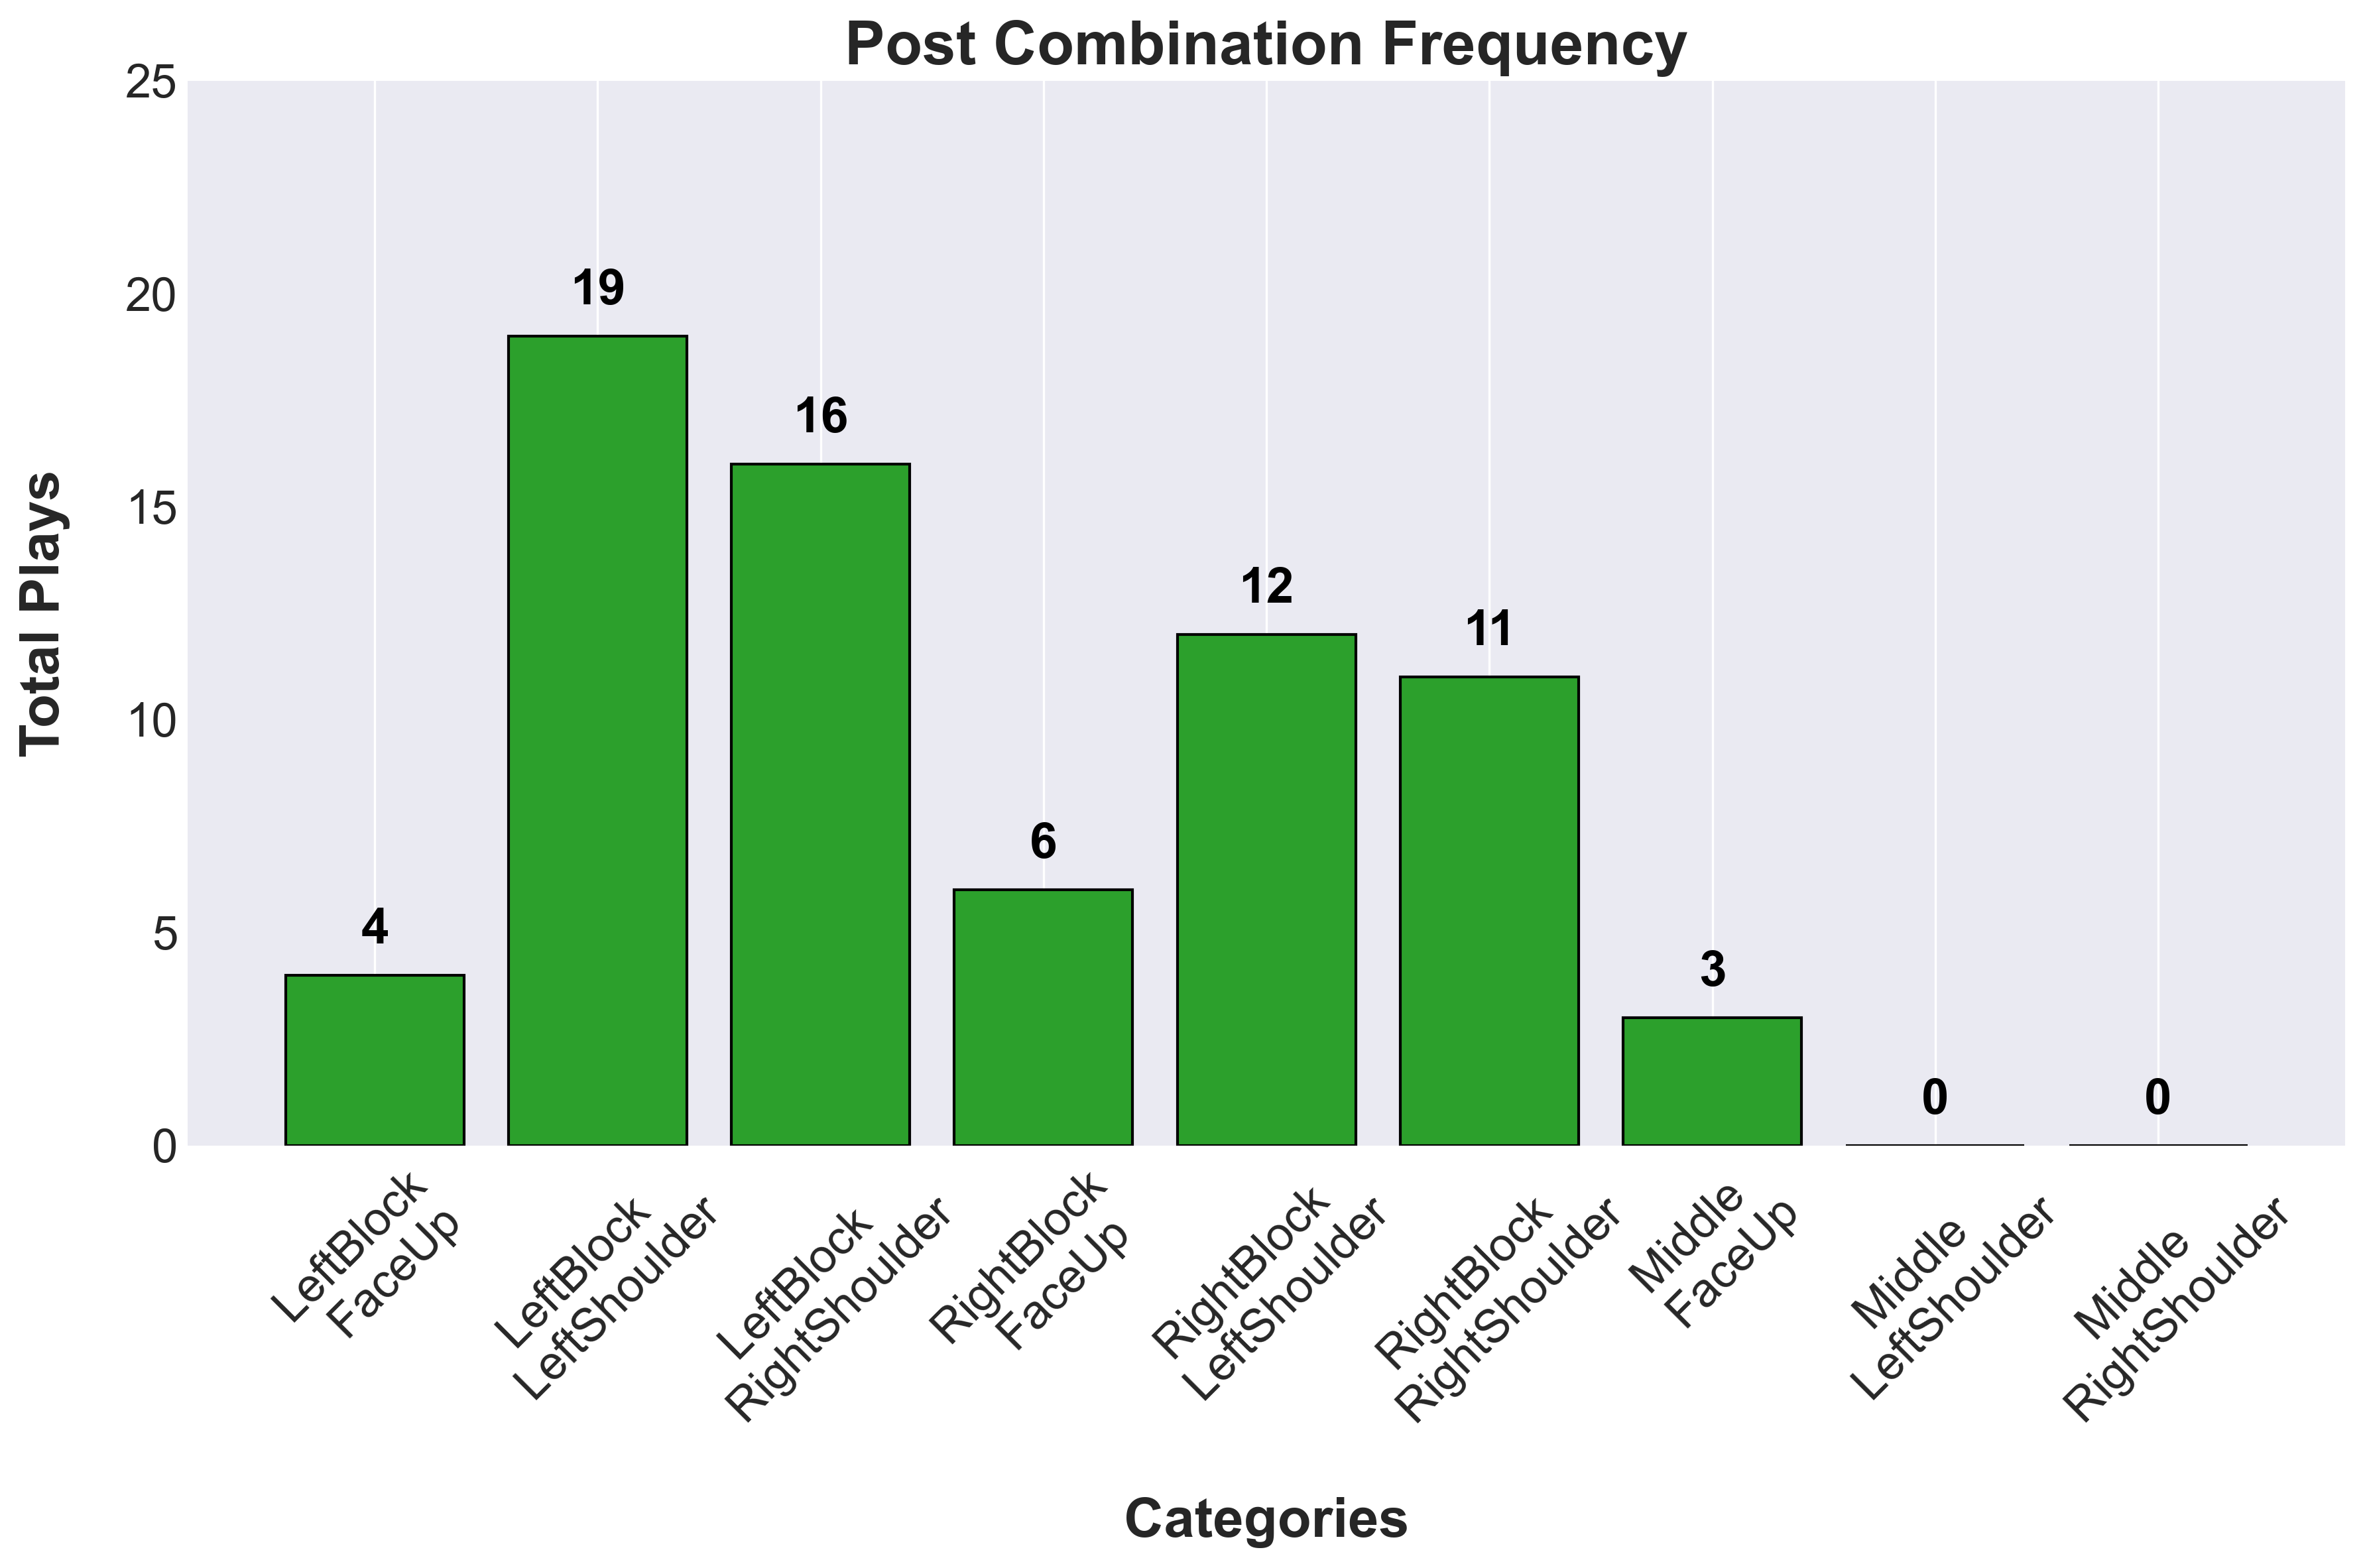
\includegraphics[width=\textwidth, height=.14\textheight]{images/Post_Combination_Freq.png} % Adjust the width of the image to fit
    \end{minipage}
\end{table}

\vspace{0em} % Add vertical space before the line (optional)
\hrule height 1pt width 1\textwidth % Adjust height and width
\vspace{1em} % Add vertical space after the line (optional)

\subsubsection{Post Passer Statistics}

\vspace{-1em} % Add vertical space before the line (optional)

% Total Post Passer Statistics
\begin{table}[H]
    \raisebox{2.5em}{ % Adjust this value to shift the tables vertically
    \begin{minipage}[t]{0.6\textwidth} % Left side (table) takes 85% of the width
        %\flushright
        \centering % Centering the title and the table
        \text{Total Post Passer Statistics} % Title above the table in bold
        \vskip .25em % Adds vertical space between title and table
        \scalebox{.85}{ % Scale the entire table down by half
            \scriptsize % Reduce the font size
            \begin{tabular}{
            >{\centering\arraybackslash}p{.75cm} 
            >{\centering\arraybackslash}p{.5cm} 
            >{\centering\arraybackslash}p{.5cm} 
            >{\centering\arraybackslash}p{.5cm}
            >{\centering\arraybackslash}p{.5cm} 
            >{\centering\arraybackslash}p{.5cm} 
            >{\centering\arraybackslash}p{.5cm} 
            >{\centering\arraybackslash}p{.5cm}
            >{\centering\arraybackslash}p{.5cm} 
            >{\centering\arraybackslash}p{.5cm}
            >{\centering\arraybackslash}p{.75cm}
            >{\centering\arraybackslash}p{.5cm} 
            >{\centering\arraybackslash}p{.5cm}}% Adjust column widths
            \toprule
            \textbf{Plays} &
            \textbf{3PA} &
            \textbf{3PM} &
            \textbf{3P\%} & 
            \textbf{2PA} & 
            \textbf{2PM} & 
            \textbf{2P\%} & 
            \textbf{MiA} & 
            \textbf{MiM} &
            \textbf{Mi\%} &
            \textbf{EFG\%} &
            \textbf{TO} &
            \textbf{Foul} \\
            \midrule
            
                
            
                
                    1 & 0 & 0 &
                    - & 
                    1 & 1 &
                    - &
                    0 & 0 &
                    - &
                    - &
                    0 & 0 \\
                
            
                
            
                
            
                
            
                
            
                
            
                
            
                
            
                
            
                
            
                
            
                
            
                
            
                
            
                
            
                
            
                
            
                
            
                
            
                
            
                
            
                
            


            \bottomrule
            \end{tabular}
        }
    \end{minipage}
    }
    \hfill % This adds some flexible space between the table and the image
    \begin{minipage}[c]{0.35\textwidth} % Right side (image) takes 10% of the width
        \flushright
        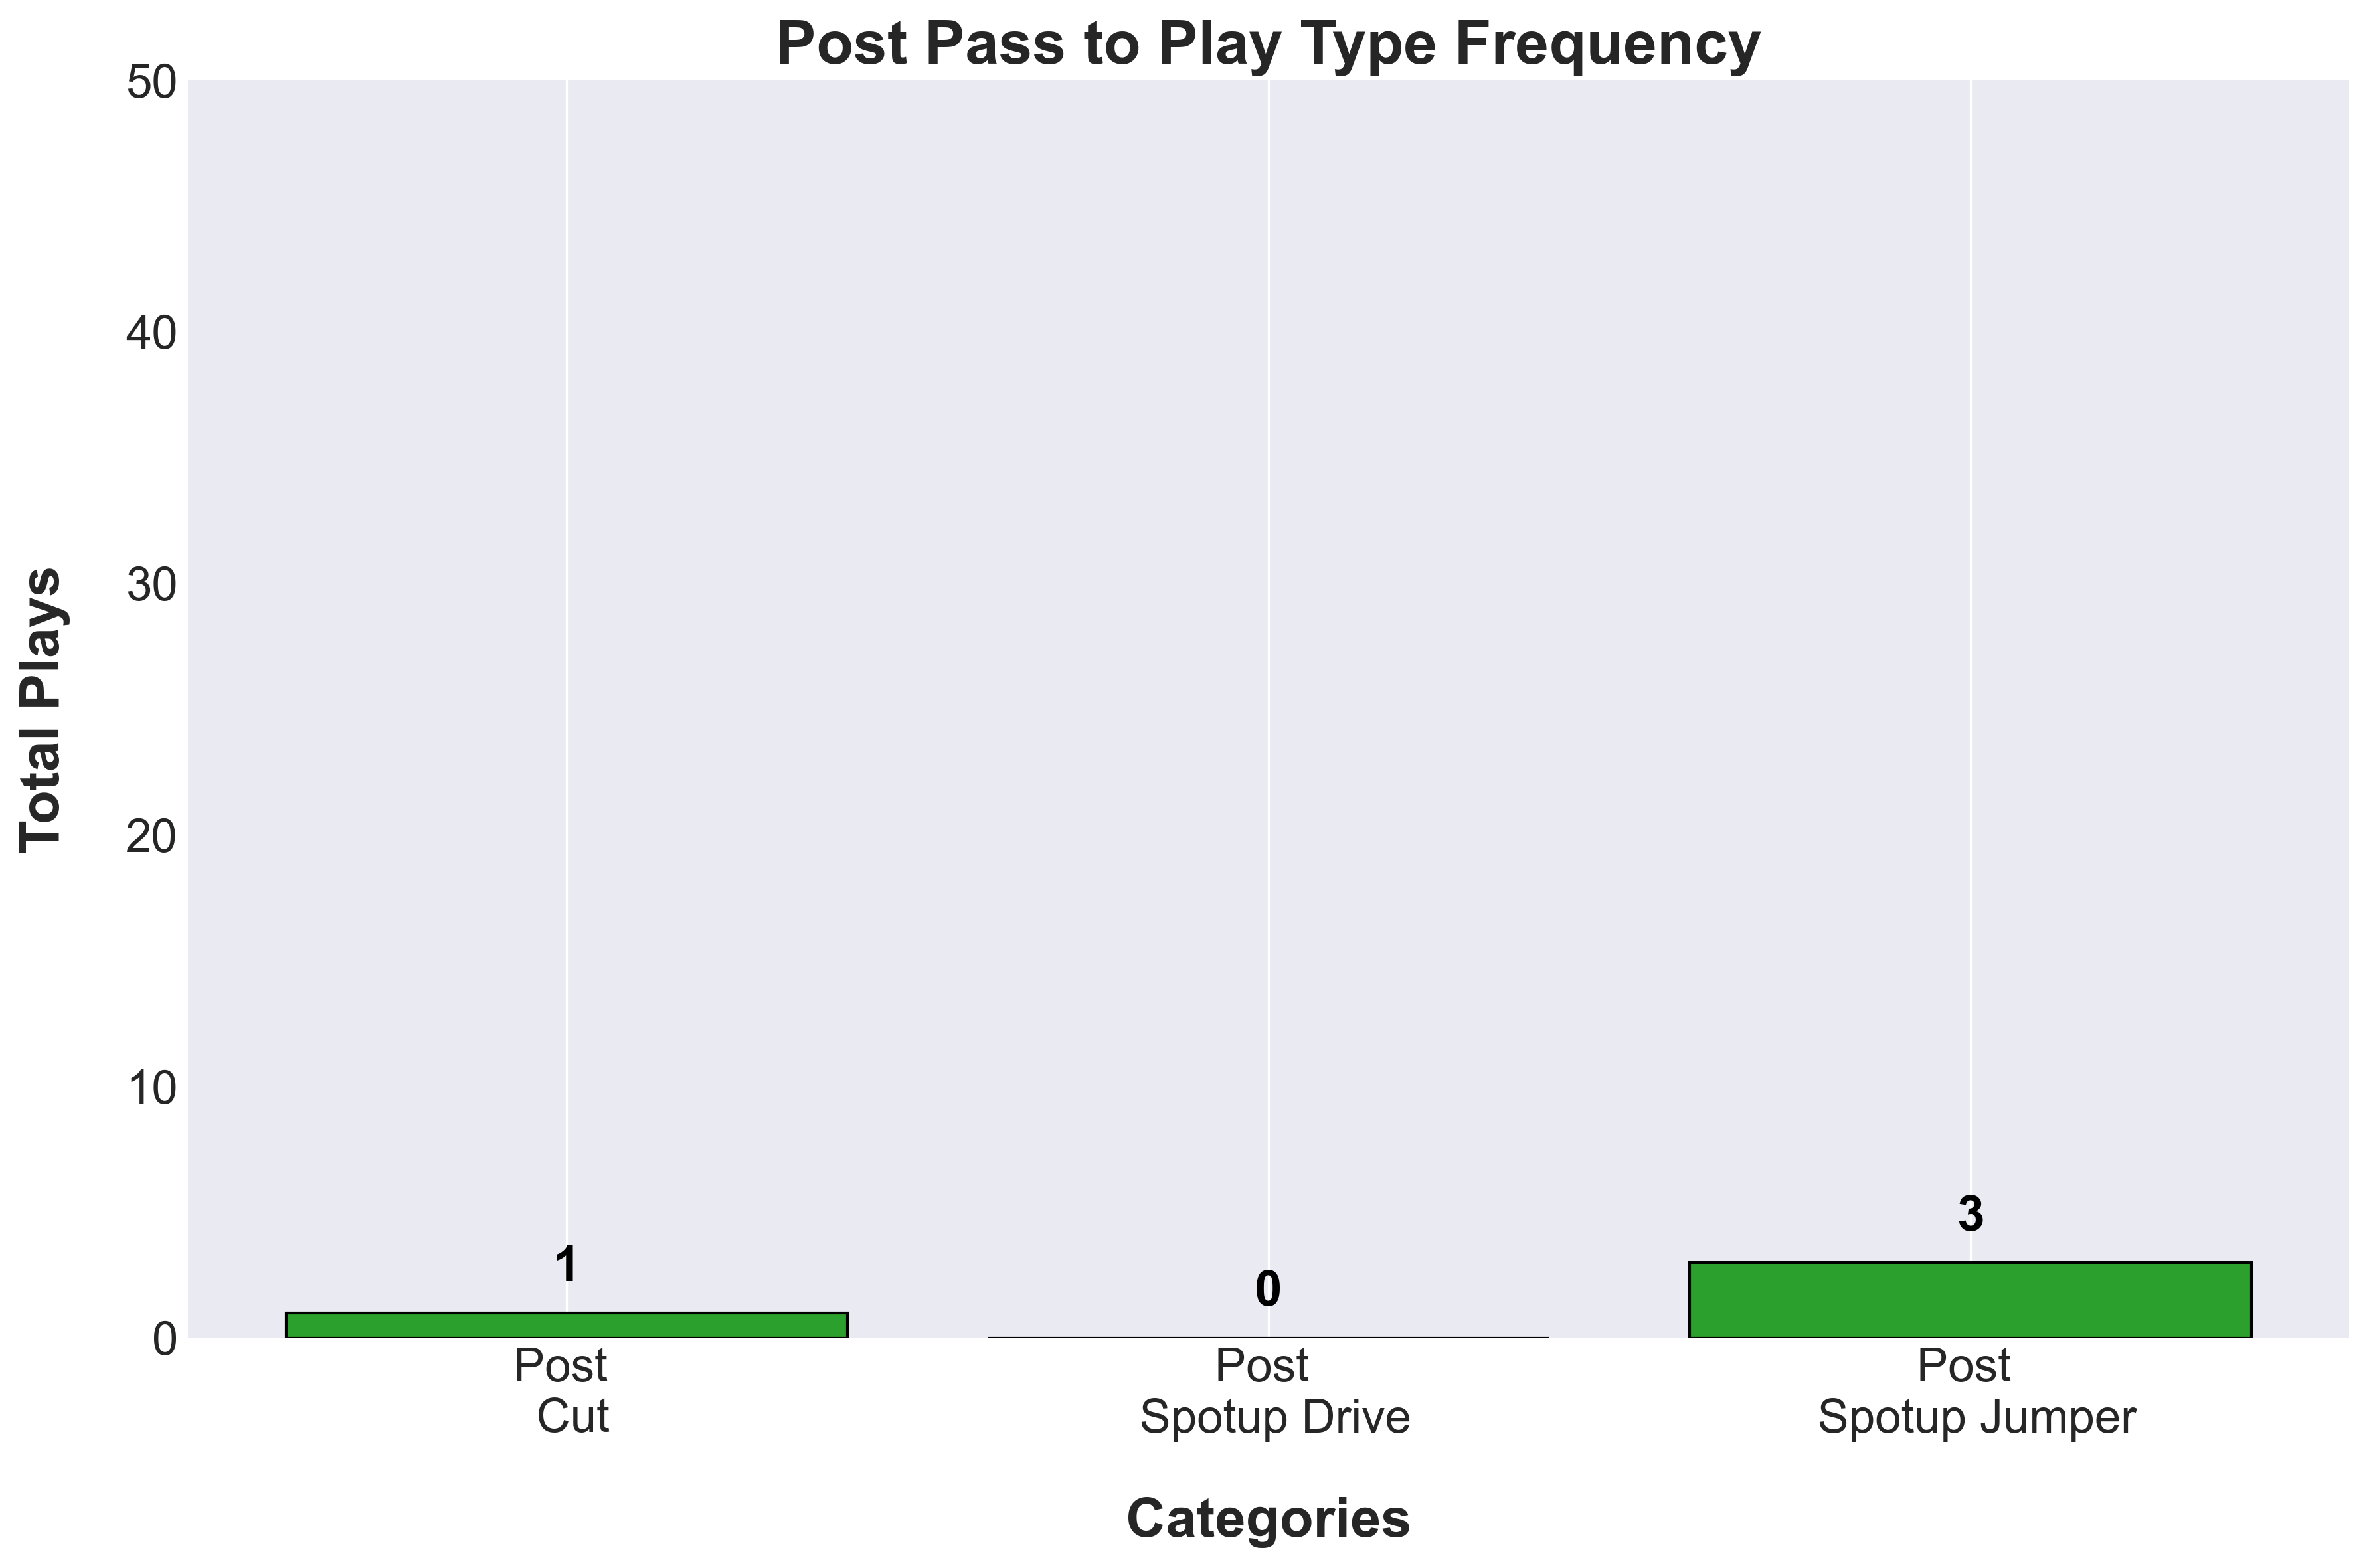
\includegraphics[width=\textwidth, height=.14\textheight]{images/Post_PassPlayType_Freq.png} % Adjust the width of the image to fit
    \end{minipage}
\end{table}

\vspace{-1em} % Add vertical space before the line (optional)
\vspace{1em} % Add vertical space after the line (optional)

% Post -> Cut Secondary Player Stats
\begin{table}[H]
    \raisebox{3em}{ % Adjust this value to shift the tables vertically
    \begin{minipage}[t]{0.6\textwidth} % Left side (table) takes 85% of the width
        \flushleft
        \centering % Centering the title and the table
        \text{Post - Cut Player Statistics} % Title above the table in bold
        \vskip .25em % Adds vertical space between title and table
        \scalebox{.55}{ % Scale the entire table down by half
            \renewcommand{\arraystretch}{1.4} % Adjust the number to increase or decrease row spacing
            \begin{tabular}{
            >{\centering\arraybackslash}p{3cm} 
            >{\centering\arraybackslash}p{.75cm} 
            >{\centering\arraybackslash}p{.75cm} 
            >{\centering\arraybackslash}p{.75cm} 
            >{\centering\arraybackslash}p{.75cm}
            >{\centering\arraybackslash}p{.75cm} 
            >{\centering\arraybackslash}p{.75cm} 
            >{\centering\arraybackslash}p{.75cm} 
            >{\centering\arraybackslash}p{.75cm} 
            >{\centering\arraybackslash}p{.75cm}}% Adjust column widths
            \toprule
            {\scriptsize \textbf{Player}} &
            {\scriptsize \textbf{Plays}} &
            {\scriptsize \textbf{2PA}} & 
            {\scriptsize \textbf{2PM}} & 
            {\scriptsize \textbf{2P\%}} & 
            {\scriptsize \textbf{MiA}} & 
            {\scriptsize \textbf{MiM}} &
            {\scriptsize \textbf{Mi\%}} &
            {\scriptsize \textbf{TO}} &
            {\scriptsize \textbf{Foul}} \\
            \midrule
            
                
            
                
            
                
                    
                        Keegan Ocorr & 
                        1 & 
                        1 & 
                        1 & 
                        - & 
                        0 & 
                        0 & 
                        - & 
                        0 & 
                        0 \\
                    
                
            
                
            
                
            
                
            
                
            
                
            
                
            
                
            
                
            
                
            
                
            
                
            
                
            
                
            
                
            
                
            
                
            
                
            
                
            
                
            
                
            

            \bottomrule
        \end{tabular}
        } % End of \scalebox
    \end{minipage}
    } % End of raisebox, closing the adjustment
    \hfill % This adds some flexible space between the table and the image
    \begin{minipage}[c]{0.35\textwidth} % Right side (image) takes 10% of the width
        \flushright
        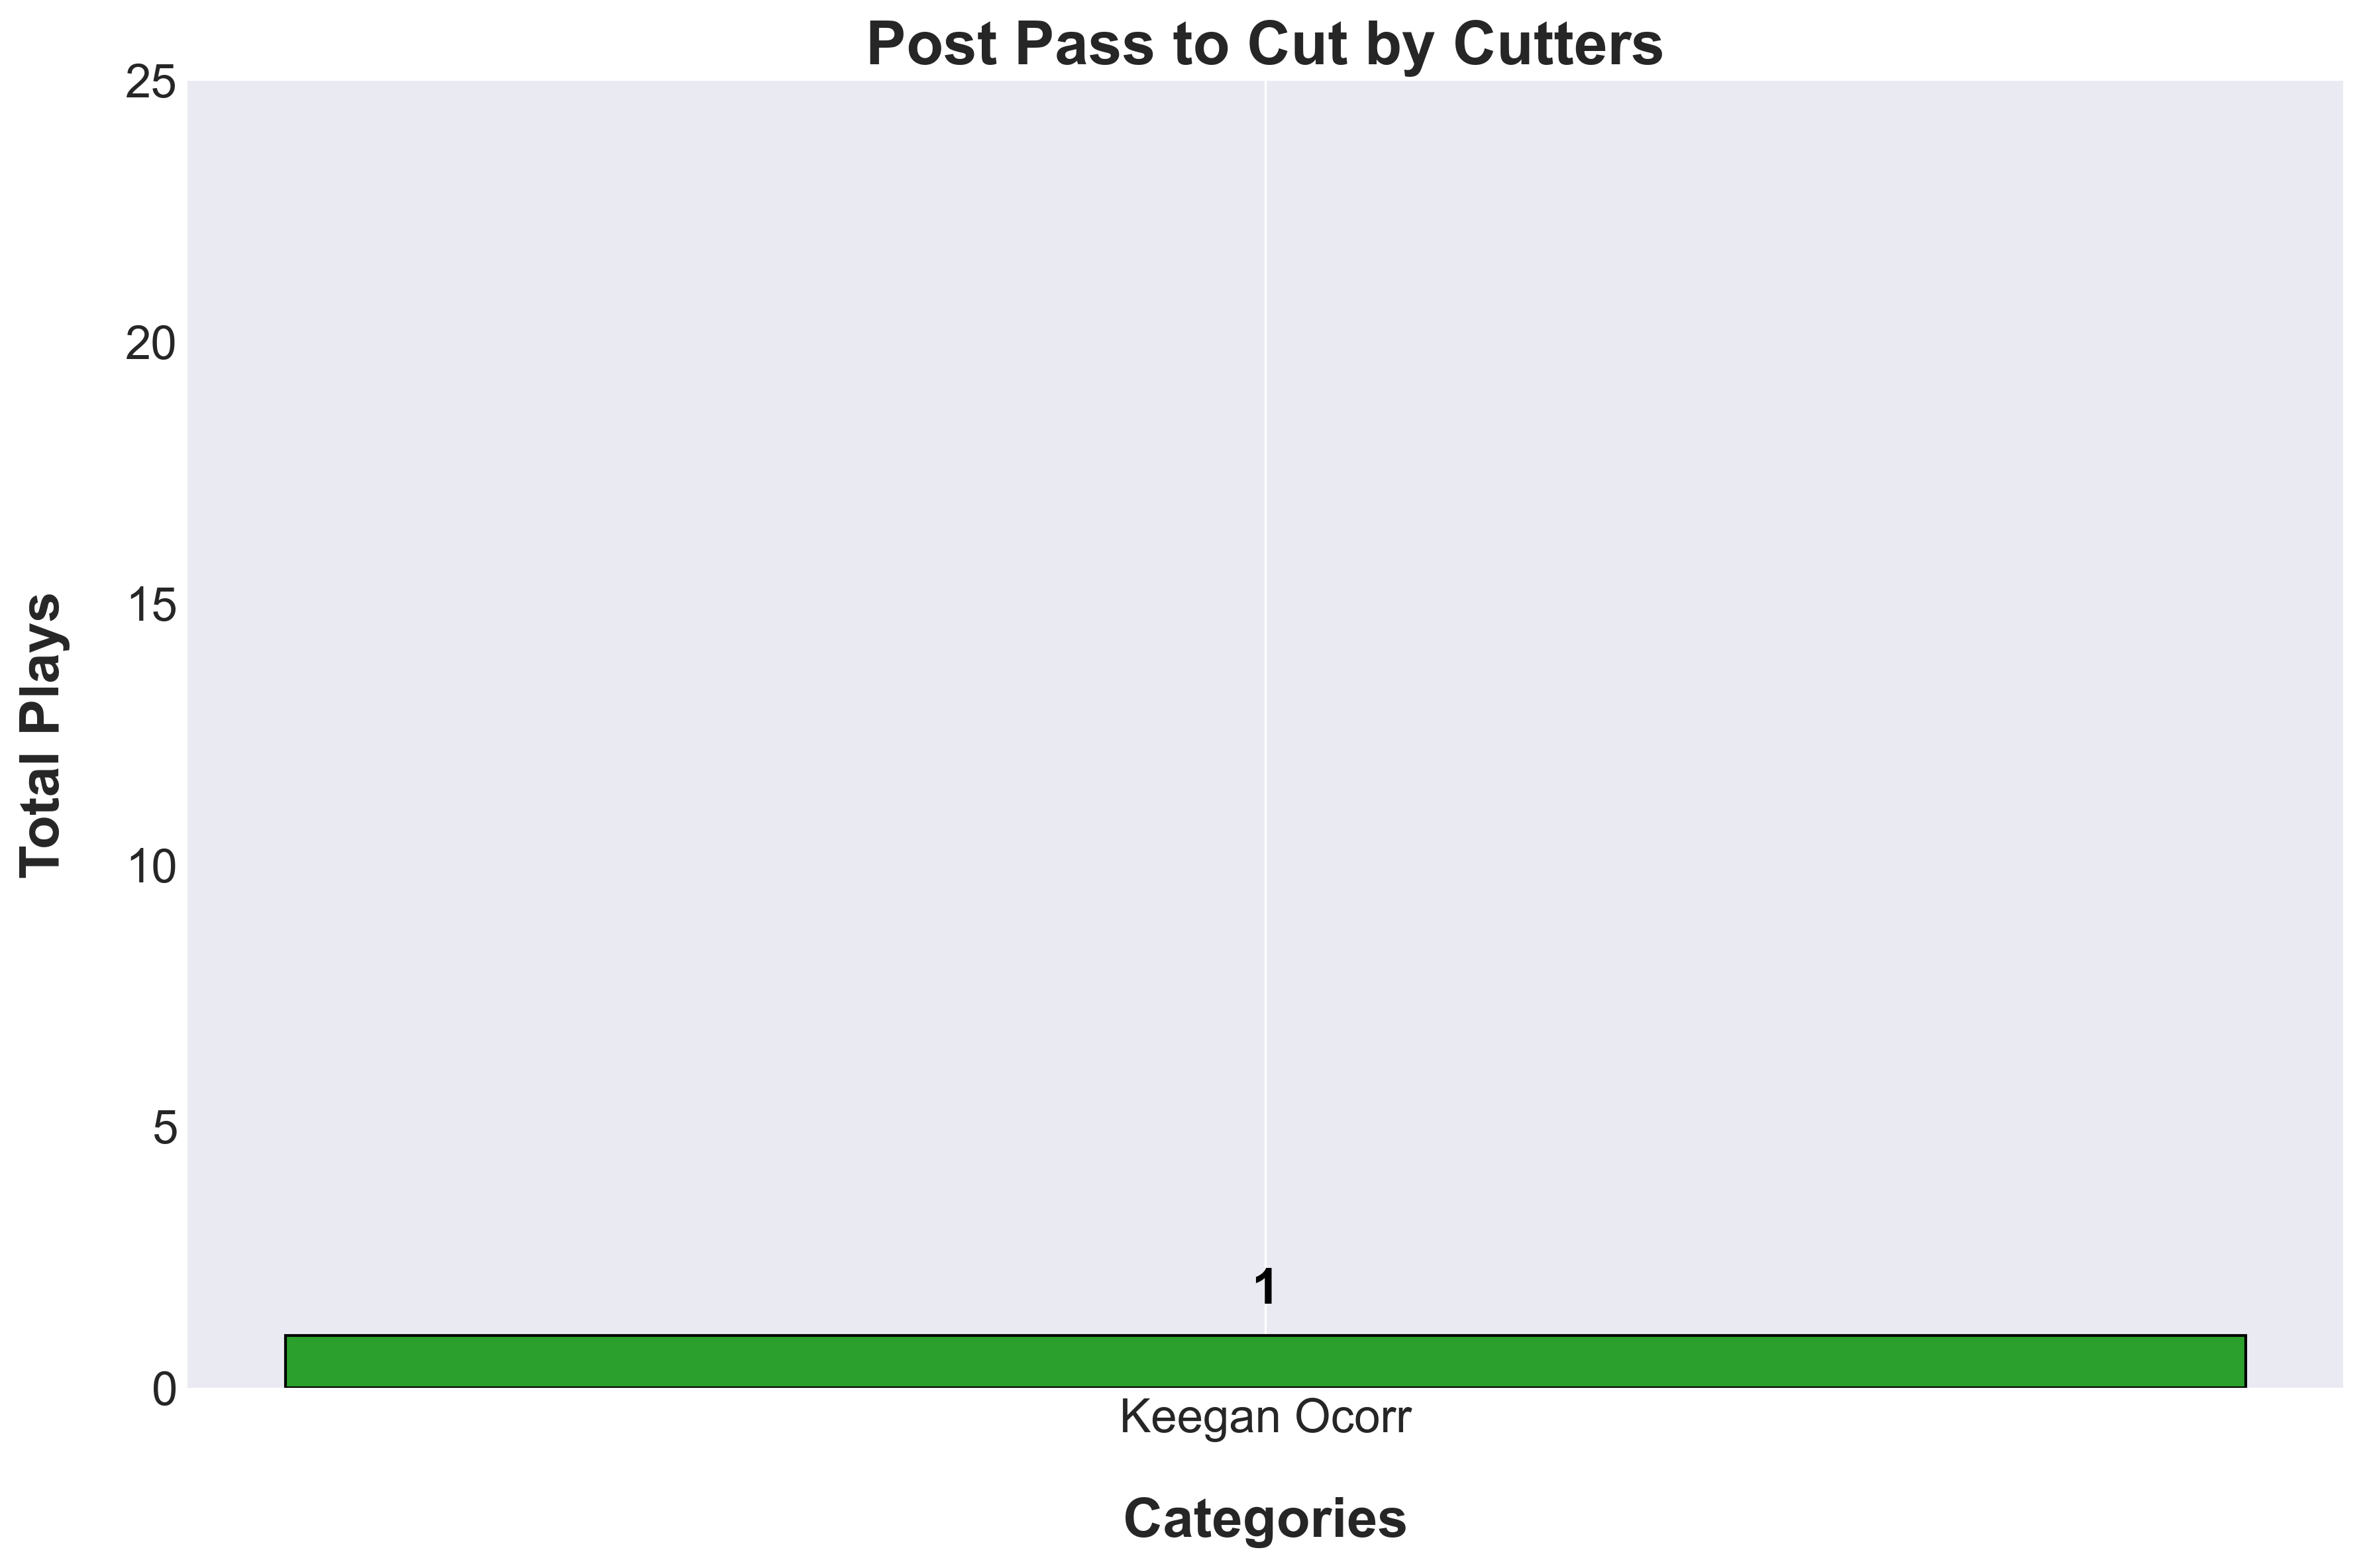
\includegraphics[width=\textwidth, height=.14\textheight]{images/Post_PassCutsPlayer_Freq.png} % Adjust the width of the image to fit
    \end{minipage}
\end{table}

\vspace{-1em} % Add vertical space before the line (optional)
\vspace{-1em} % Add vertical space after the line (optional)

% Post -> Spot Up Drives Secondary Player Stats
\begin{table}[H]
    \raisebox{3em}{ % Adjust this value to shift the tables vertically
    \begin{minipage}[t]{0.6\textwidth} % Left side (table) takes 85% of the width
        \flushleft
        \centering % Centering the title and the table
        \text{Post - Spot Up Drives Player Statistics} % Title above the table in bold
        \vskip .25em % Adds vertical space between title and table
        \scalebox{.55}{ % Scale the entire table down by half
            \renewcommand{\arraystretch}{1.4} % Adjust the number to increase or decrease row spacing
            \begin{tabular}{
            >{\centering\arraybackslash}p{3cm} 
            >{\centering\arraybackslash}p{.75cm} 
            >{\centering\arraybackslash}p{.75cm} 
            >{\centering\arraybackslash}p{.75cm} 
            >{\centering\arraybackslash}p{.75cm}
            >{\centering\arraybackslash}p{.75cm} 
            >{\centering\arraybackslash}p{.75cm} 
            >{\centering\arraybackslash}p{.75cm} 
            >{\centering\arraybackslash}p{.75cm}
            >{\centering\arraybackslash}p{.75cm} 
            >{\centering\arraybackslash}p{.75cm}
            >{\centering\arraybackslash}p{.75cm}
            >{\centering\arraybackslash}p{.75cm} 
            >{\centering\arraybackslash}p{.75cm}}% Adjust column widths
            \toprule
            {\scriptsize \textbf{Player}} &
            {\scriptsize \textbf{Plays}} &
            {\scriptsize \textbf{3PA}} &
            {\scriptsize \textbf{3PM}} &
            {\scriptsize \textbf{3P\%}} & 
            {\scriptsize \textbf{2PA}} & 
            {\scriptsize \textbf{2PM}} & 
            {\scriptsize \textbf{2P\%}} & 
            {\scriptsize \textbf{MiA}} & 
            {\scriptsize \textbf{MiM}} &
            {\scriptsize \textbf{Mi\%}} &
            {\scriptsize \textbf{EFG\%}} &
            {\scriptsize \textbf{TO}} &
            {\scriptsize \textbf{Foul}} \\
            \midrule
            
                
            
                
            
                
            
                
                    
                
            
                
            
                
            
                
            
                
            
                
            
                
            
                
            
                
            
                
            
                
            
                
            
                
            
                
            
                
            
                
            
                
            
                
            
                
            
                
            

            \bottomrule
        \end{tabular}
        } % End of \scalebox
    \end{minipage}
    } % End of raisebox, closing the adjustment
    \hfill % This adds some flexible space between the table and the image
    \begin{minipage}[c]{0.35\textwidth} % Right side (image) takes 10% of the width
        \flushright
        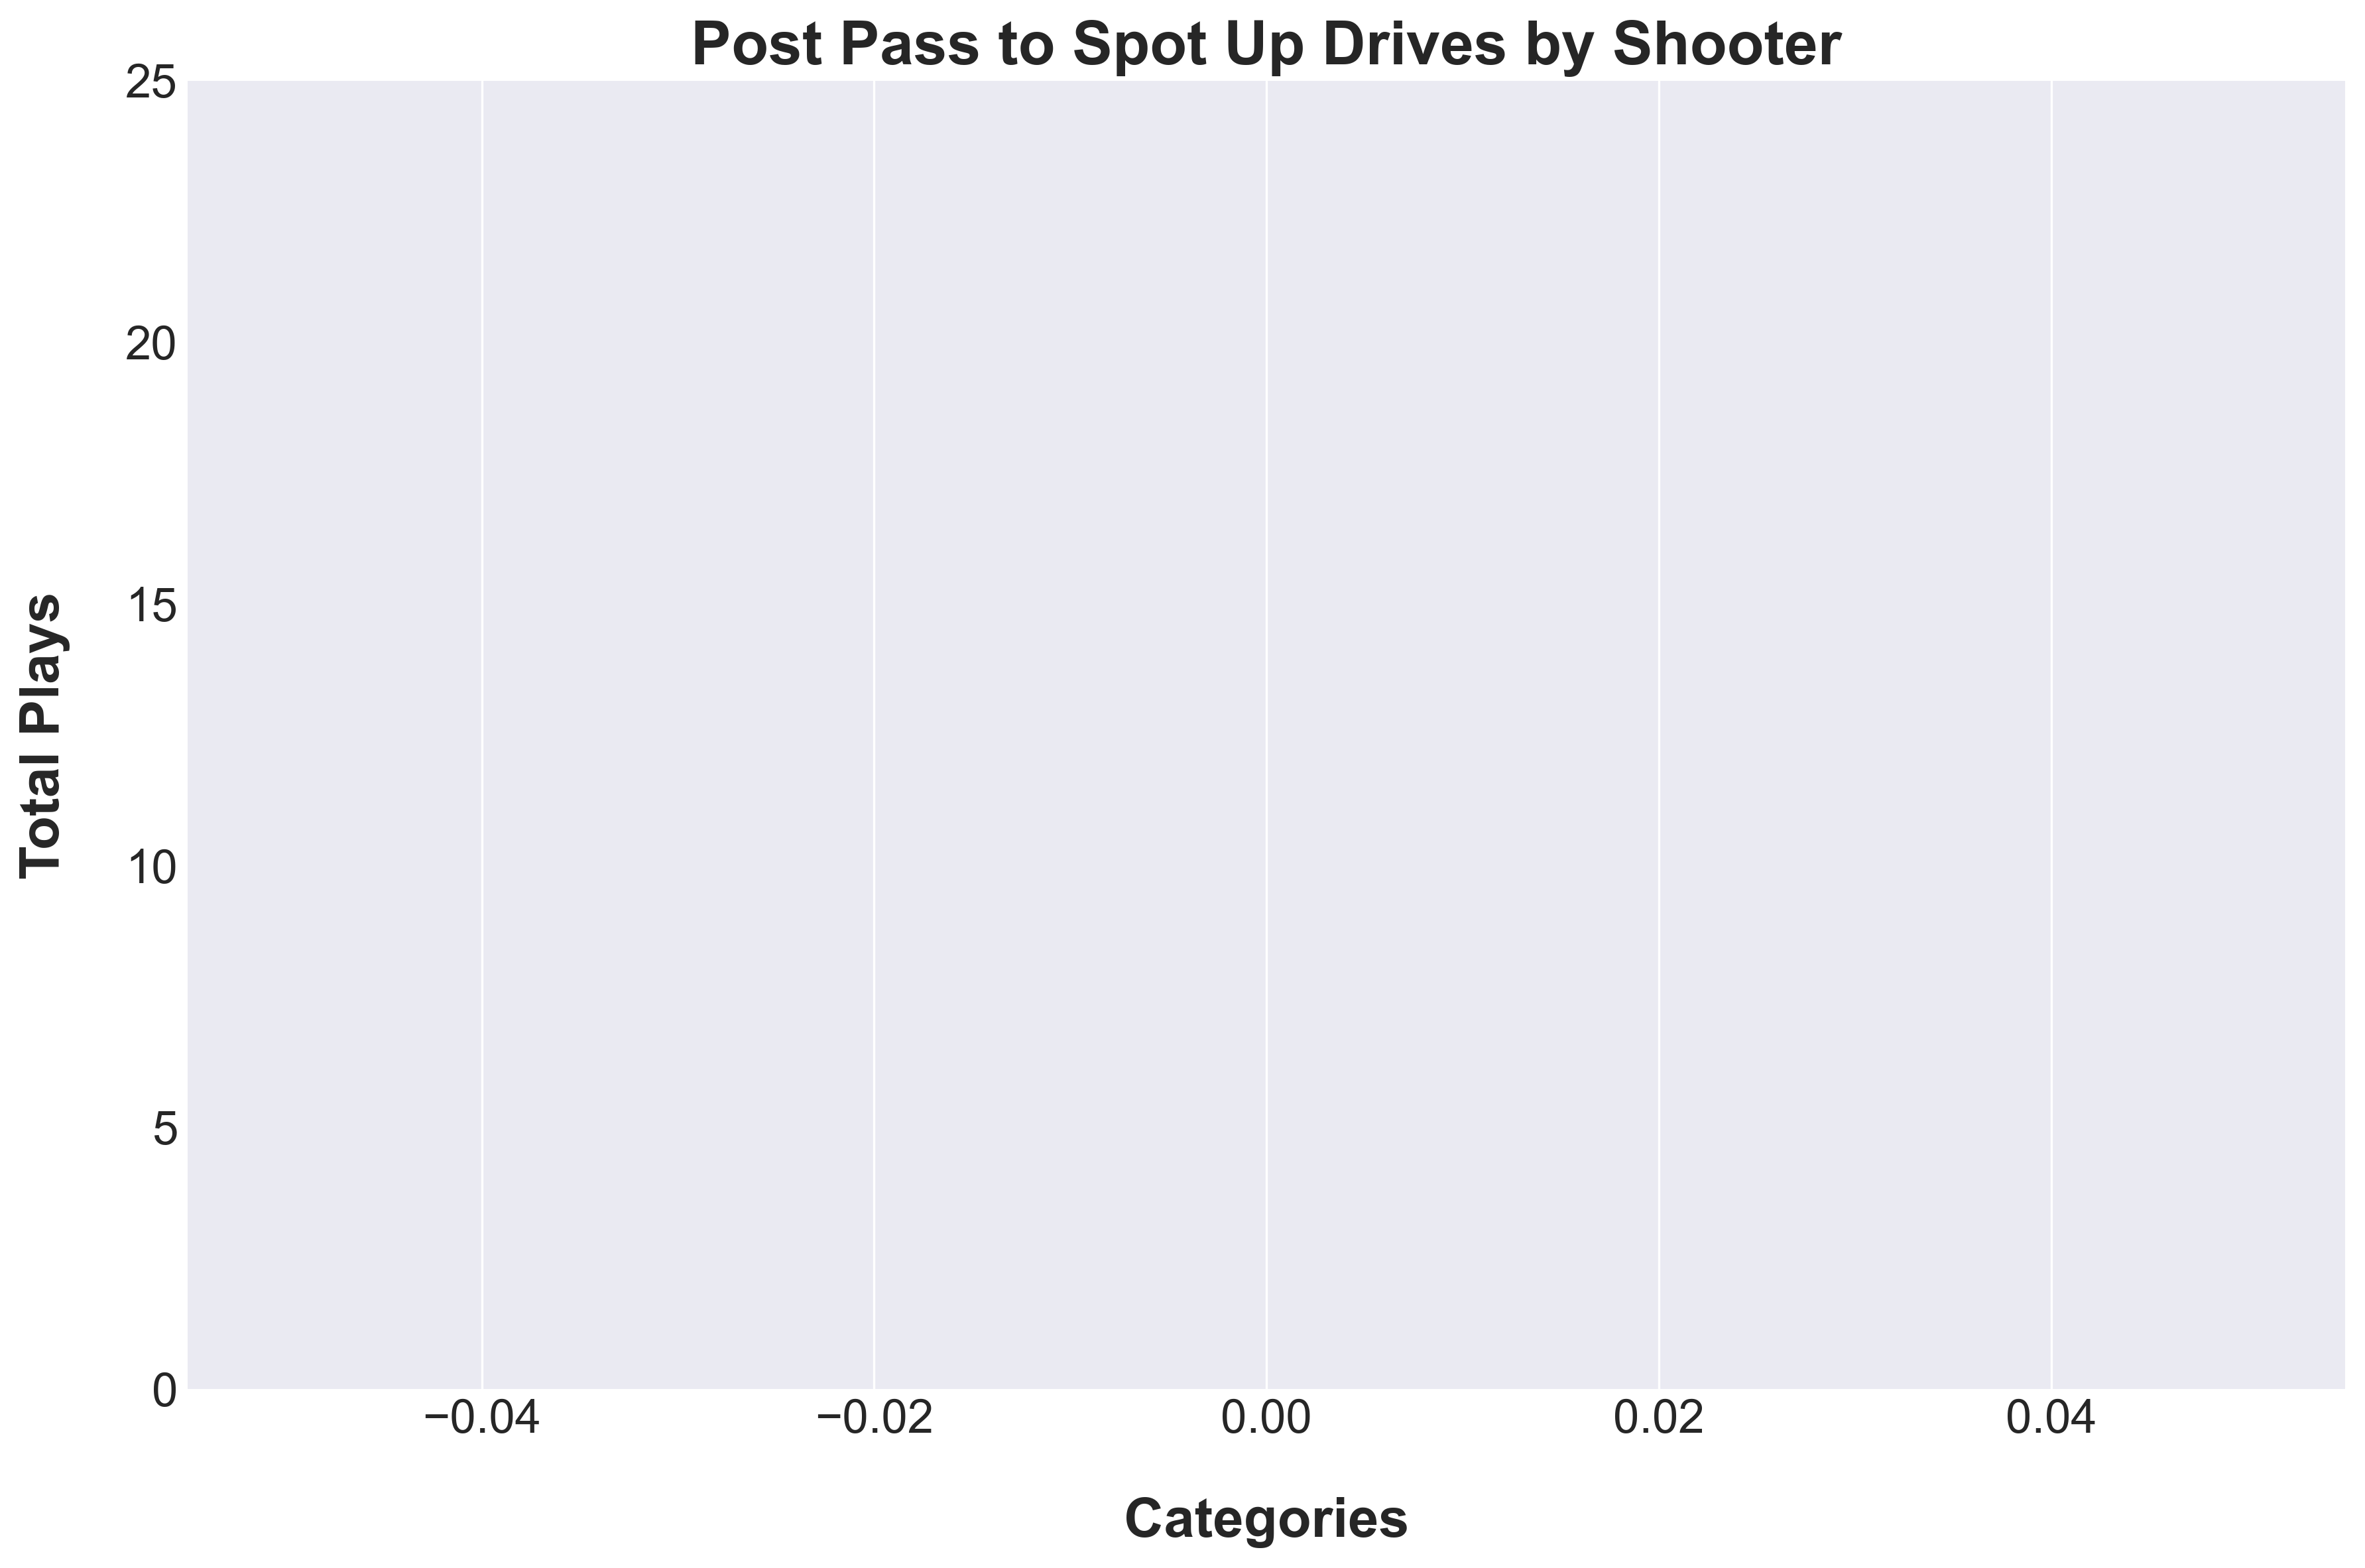
\includegraphics[width=\textwidth, height=.14\textheight]{images/Post_PassDrivesPlayer_Freq.png} % Adjust the width of the image to fit
    \end{minipage}
\end{table}

\vspace{-1em} % Add vertical space before the line (optional)
\vspace{-1em} % Add vertical space after the line (optional)

% Post -> Spot Up Jumpers Secondary Player Stats
\begin{table}[H]
    \raisebox{3em}{ % Adjust this value to shift the tables vertically
    \begin{minipage}[t]{0.6\textwidth} % Left side (table) takes 85% of the width
        \flushleft
        \centering % Centering the title and the table
        \text{Post - Spot Up Jumpers Player Statistics} % Title above the table in bold
        \vskip .25em % Adds vertical space between title and table
        \scalebox{.55}{ % Scale the entire table down by half
            \renewcommand{\arraystretch}{1.4} % Adjust the number to increase or decrease row spacing
            \begin{tabular}{
            >{\centering\arraybackslash}p{3cm} 
            >{\centering\arraybackslash}p{.75cm} 
            >{\centering\arraybackslash}p{.75cm} 
            >{\centering\arraybackslash}p{.75cm} 
            >{\centering\arraybackslash}p{.75cm} 
            >{\centering\arraybackslash}p{.75cm}
            >{\centering\arraybackslash}p{.75cm} 
            >{\centering\arraybackslash}p{.75cm}
            >{\centering\arraybackslash}p{.75cm}
            >{\centering\arraybackslash}p{.75cm} 
            >{\centering\arraybackslash}p{.75cm}}% Adjust column widths
            \toprule
            {\scriptsize \textbf{Player}} &
            {\scriptsize \textbf{Plays}} &
            {\scriptsize \textbf{3PA}} &
            {\scriptsize \textbf{3PM}} &
            {\scriptsize \textbf{3P\%}} & 
            {\scriptsize \textbf{MiA}} & 
            {\scriptsize \textbf{MiM}} &
            {\scriptsize \textbf{Mi\%}} &
            {\scriptsize \textbf{EFG\%}} &
            {\scriptsize \textbf{TO}} &
            {\scriptsize \textbf{Foul}} \\
            \midrule
            
                
            
                
            
                
            
                
            
                
                    
                
            
                
            
                
            
                
            
                
            
                
            
                
            
                
            
                
            
                
            
                
            
                
            
                
            
                
            
                
            
                
            
                
            
                
            
                
            

            \bottomrule
        \end{tabular}
        } % End of \scalebox
    \end{minipage}
    } % End of raisebox, closing the adjustment
    \hfill % This adds some flexible space between the table and the image
    \begin{minipage}[c]{0.35\textwidth} % Right side (image) takes 10% of the width
        \flushright
        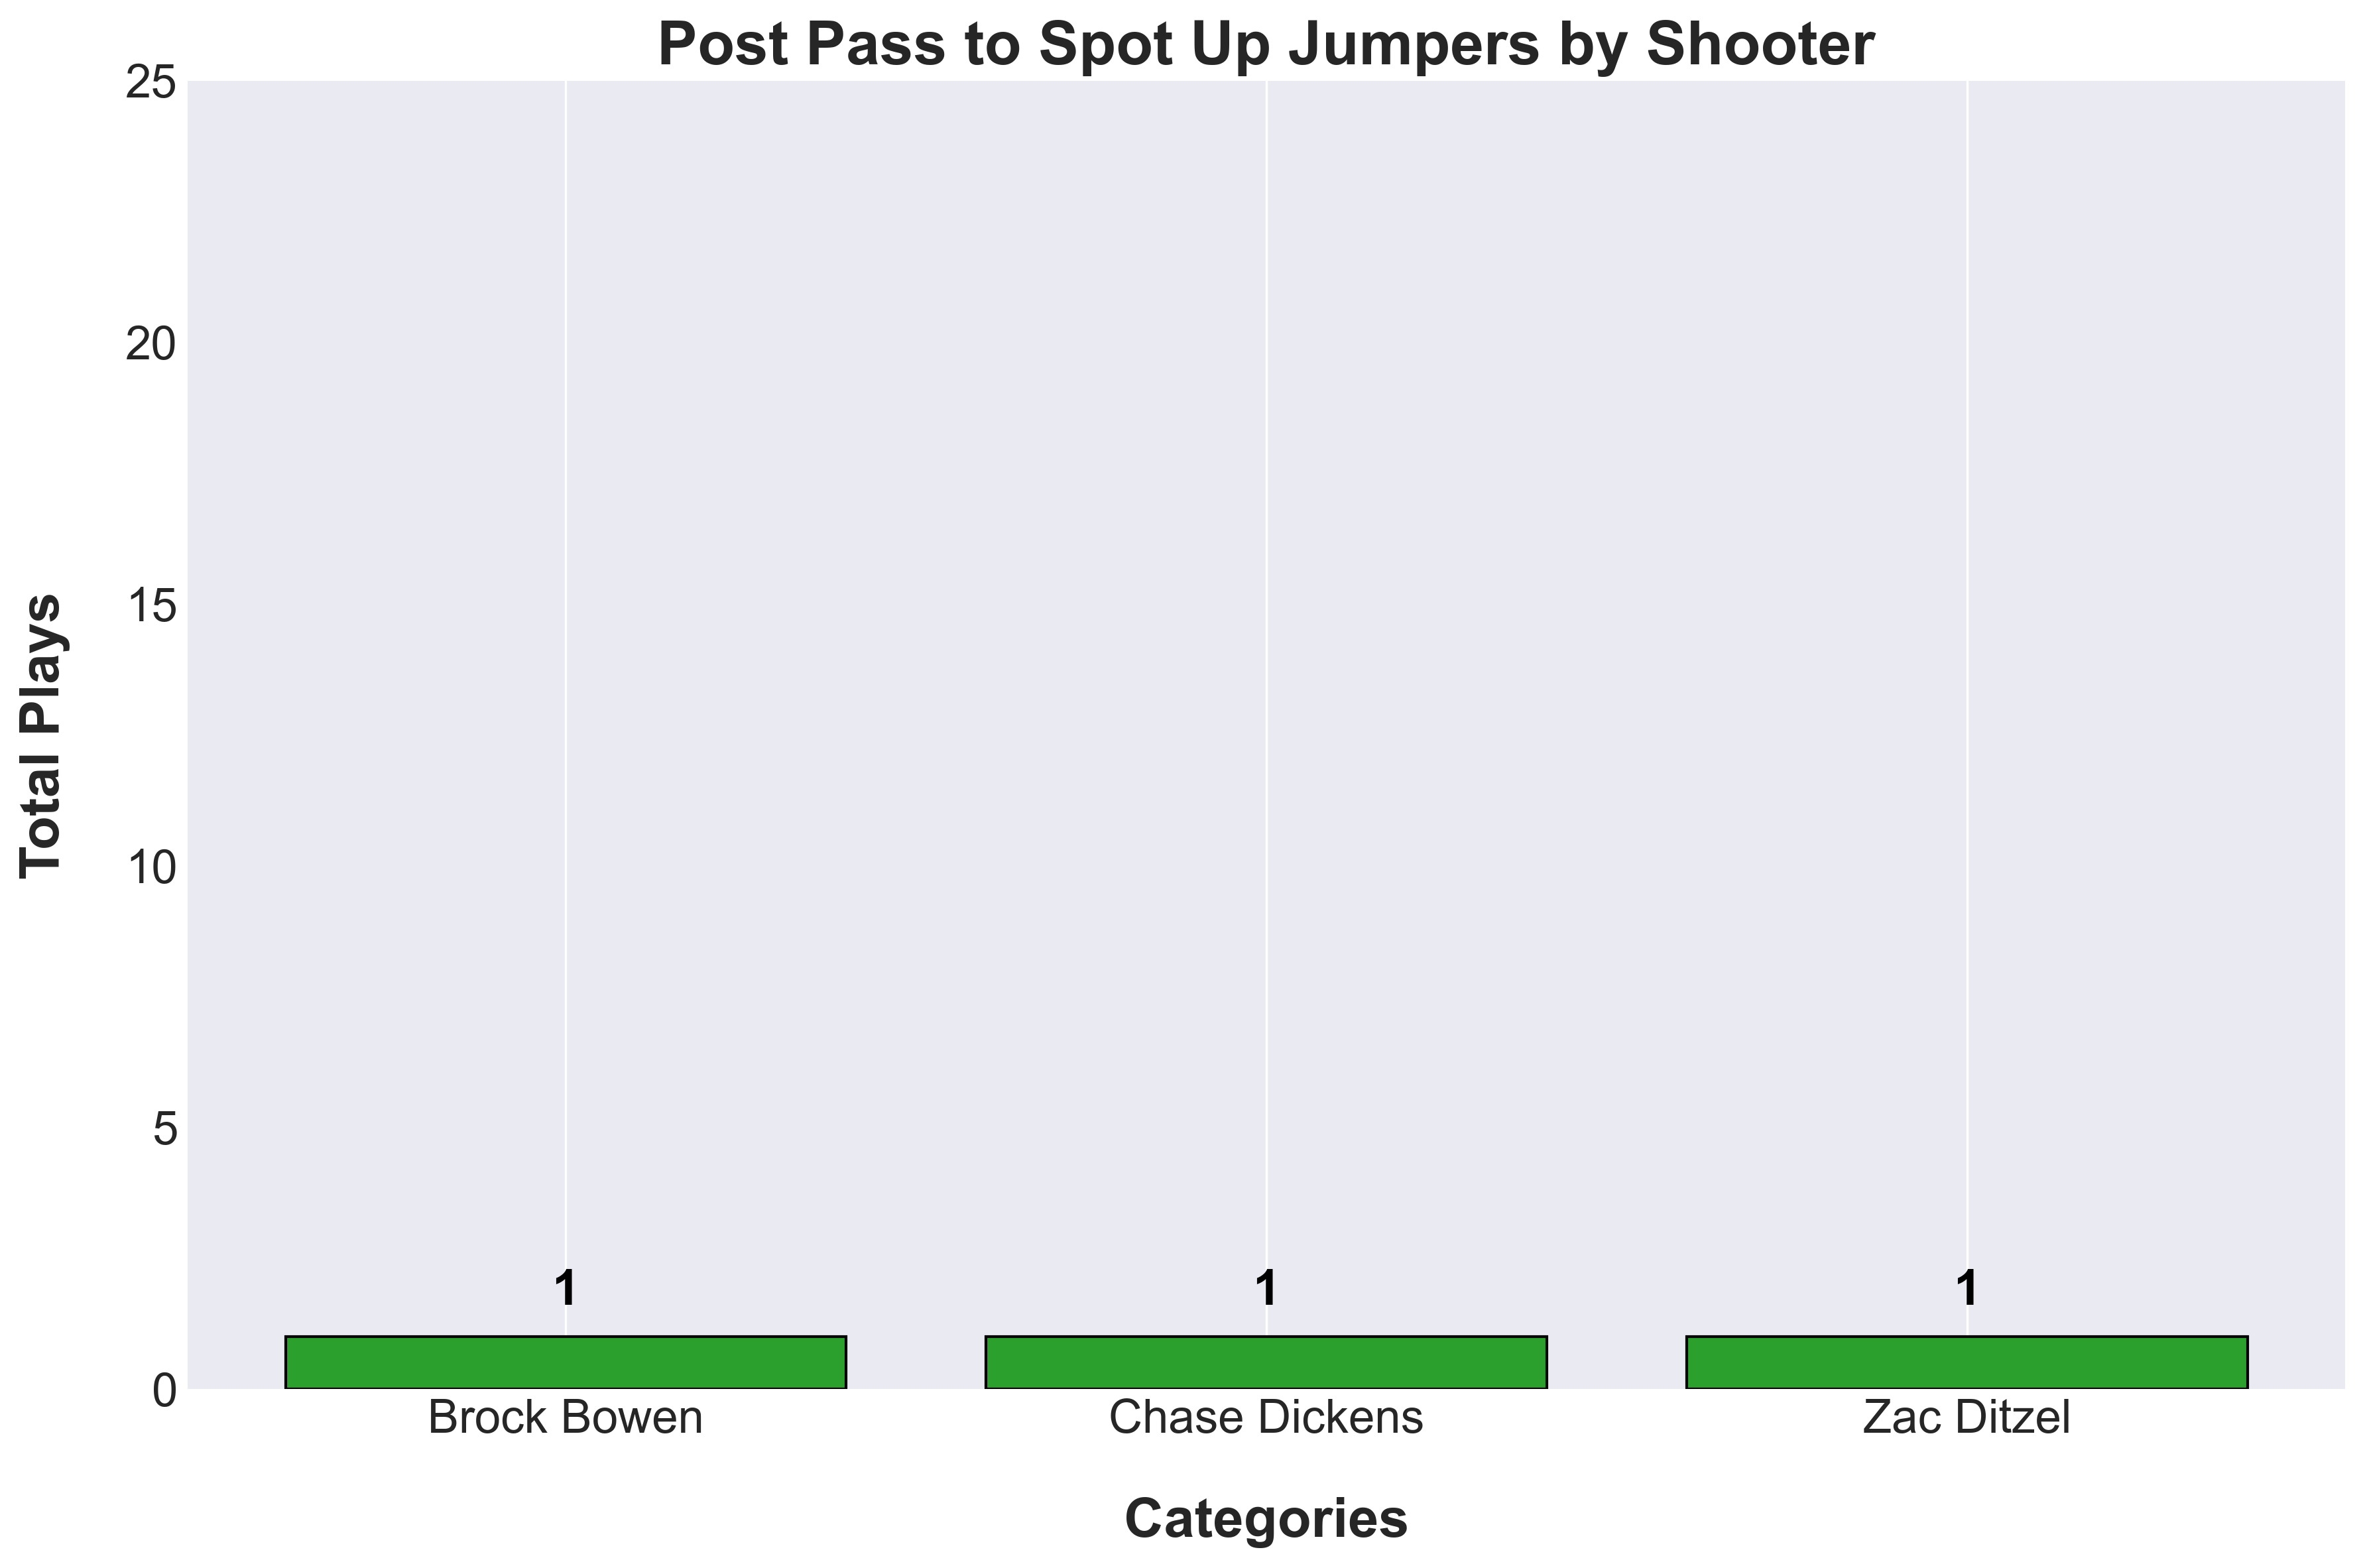
\includegraphics[width=\textwidth, height=.14\textheight]{images/Post_PassShotsPlayer_Freq.png} % Adjust the width of the image to fit
    \end{minipage}
\end{table}

\vspace{-1em} % Add vertical space before the line (optional)
\hrule height 1pt width 1\textwidth % Adjust height and width
\vspace{1em} % Add vertical space after the line (optional)

\clearpage




% ----------------------
% Rollman Visuals and Insights Section
% ----------------------
\subsection{Rollman}\

\vspace{0.25em} % Add vertical space before the line (optional)
\textbf{Key Notes on Rollman Tendencies}
\vspace{0.5em} % Add space between the title and the itemized list

\begin{itemize}
    \item Rollman Plays make up x\% of players offensive load
    \vspace{0.3em} % Add space between the title and the itemized list
    \item Player is more efficient shooting over his left shoulder and get shots off of the left block x\% of the time which is much higher than the middle and right block.
\end{itemize}

\vspace{1em} % Add vertical space after the line (optional)
\hrule height 1pt width 1\textwidth % Adjust height and width
\vspace{0em} % Add vertical space after the line (optional)

\subsubsection{Rollman General Scorer Stats}
% All Rollman Statistics Table w/ room for insights
\begin{table}[H]
    \centering
    \begin{minipage}[t]{0.6\textwidth} % Left side (table) takes 85% of the width
        %\flushright
        \centering % Centering the title and the table
        \text{Total Rollman Shot Statistics} % Title above the table in bold
        \vskip .25em % Adds vertical space between title and table
        \scalebox{.85}{ % Scale the entire table down by half
            \scriptsize % Reduce the font size
            \begin{tabular}{
            >{\centering\arraybackslash}p{.75cm} 
            >{\centering\arraybackslash}p{.5cm} 
            >{\centering\arraybackslash}p{.5cm} 
            >{\centering\arraybackslash}p{.5cm}
            >{\centering\arraybackslash}p{.5cm} 
            >{\centering\arraybackslash}p{.5cm} 
            >{\centering\arraybackslash}p{.5cm} 
            >{\centering\arraybackslash}p{.5cm}
            >{\centering\arraybackslash}p{.5cm} 
            >{\centering\arraybackslash}p{.5cm}
            >{\centering\arraybackslash}p{.75cm}
            >{\centering\arraybackslash}p{.5cm} 
            >{\centering\arraybackslash}p{.5cm}}% Adjust column widths
            \toprule
            \textbf{Plays} &
            \textbf{3PA} &
            \textbf{3PM} &
            \textbf{3P\%} & 
            \textbf{2PA} & 
            \textbf{2PM} & 
            \textbf{2P\%} & 
            \textbf{MiA} & 
            \textbf{MiM} &
            \textbf{Mi\%} &
            \textbf{EFG\%} &
            \textbf{TO} &
            \textbf{Foul} \\
            \midrule
            
                
            
                
            
                
            
                
            
                
            
                
            
                
            
                
            
                
            
                
            
                
            
                
            
                
            
                
            
                
            
                
            

            \bottomrule
            \end{tabular}
        }
    \end{minipage}
\end{table}

\vspace{0em} % Add vertical space before the line (optional)
%\hrule height 1pt width 1\textwidth % Adjust height and width
\vspace{-1em} % Add vertical space after the line (optional)

% Rollman Stats for Slip vs Pop vs Roll 
\begin{table}[H]
    \raisebox{3em}{ % Adjust this value to shift the tables vertically
    \begin{minipage}[t]{0.6\textwidth} % Left side (table) takes 85% of the width
        \flushleft
        \centering % Centering the title and the table
        \text{Rollman Play Type Statistics} % Title above the table in bold
        \vskip .25em % Adds vertical space between title and table
        \scalebox{.6}{ % Scale the entire table down by half
            \renewcommand{\arraystretch}{1.4} % Adjust the number to increase or decrease row spacing
            \begin{tabular}{
            >{\centering\arraybackslash}p{1.75cm} 
            >{\centering\arraybackslash}p{.75cm} 
            >{\centering\arraybackslash}p{.75cm} 
            >{\centering\arraybackslash}p{.75cm} 
            >{\centering\arraybackslash}p{.75cm}
            >{\centering\arraybackslash}p{.75cm} 
            >{\centering\arraybackslash}p{.75cm} 
            >{\centering\arraybackslash}p{.75cm} 
            >{\centering\arraybackslash}p{.75cm}
            >{\centering\arraybackslash}p{.75cm} 
            >{\centering\arraybackslash}p{.75cm}
            >{\centering\arraybackslash}p{.75cm}
            >{\centering\arraybackslash}p{.75cm} 
            >{\centering\arraybackslash}p{.75cm}}% Adjust column widths
            \toprule
            {\scriptsize \textbf{PlayType}} &
            {\scriptsize \textbf{Plays}} &
            {\scriptsize \textbf{3PA}} &
            {\scriptsize \textbf{3PM}} &
            {\scriptsize \textbf{3P\%}} & 
            {\scriptsize \textbf{2PA}} & 
            {\scriptsize \textbf{2PM}} & 
            {\scriptsize \textbf{2P\%}} & 
            {\scriptsize \textbf{MiA}} & 
            {\scriptsize \textbf{MiM}} &
            {\scriptsize \textbf{Mi\%}} &
            {\scriptsize \textbf{EFG\%}} &
            {\scriptsize \textbf{TO}} &
            {\scriptsize \textbf{Foul}} \\
            \midrule
            
                
            
                
            
                
            
                
            
                
            
                
            
                
            
                
            
                
            
                
            
                
            
                
            
                
            
                
            
                
            
                
            


            \bottomrule
        \end{tabular}
        } % End of \scalebox
    \end{minipage}
    } % End of raisebox, closing the adjustment
    \hfill % This adds some flexible space between the table and the image
    \begin{minipage}[c]{0.35\textwidth} % Right side (image) takes 10% of the width
        \flushright
        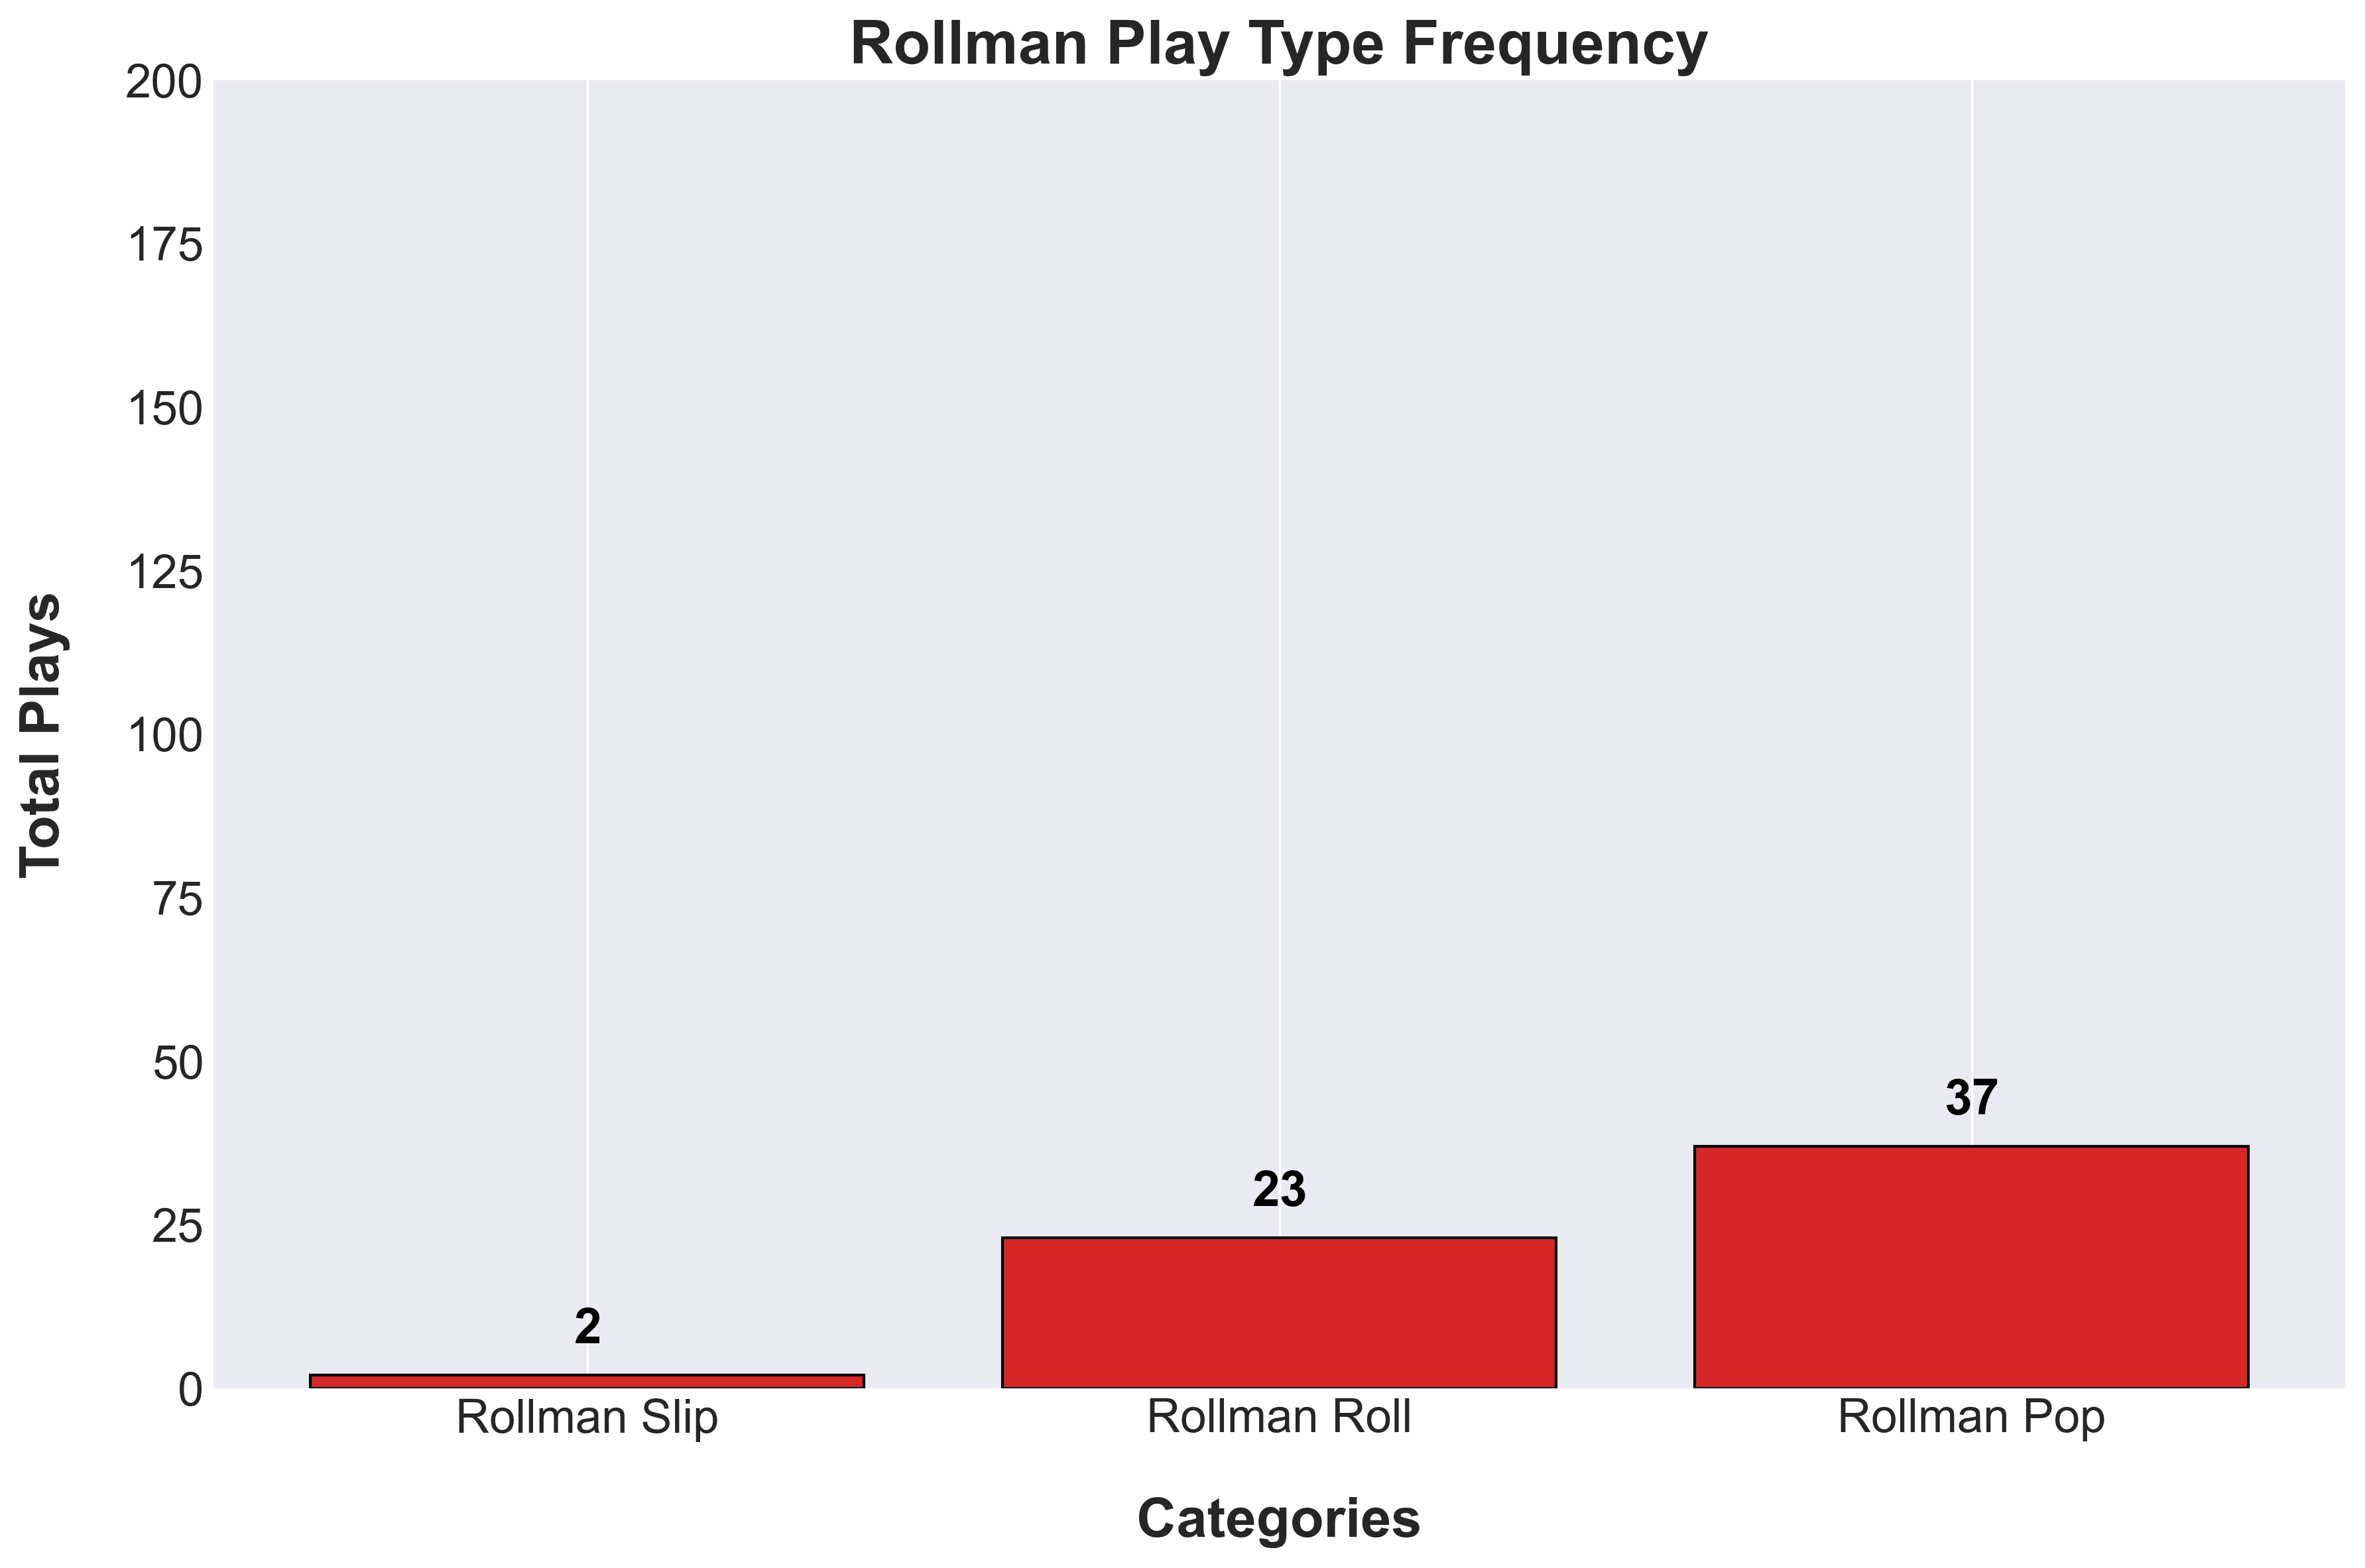
\includegraphics[width=\textwidth, height=.14\textheight]{images/Rollman_PlayType_Freq.png} % Adjust the width of the image to fit
    \end{minipage}
\end{table}

\vspace{-1em} % Add vertical space before the line (optional)
%\hrule height 1pt width 1\textwidth % Adjust height and width
\vspace{-1em} % Add vertical space after the line (optional)

% Rollman Slip Drive Direction
\begin{table}[H]
    \raisebox{3.5em}{ % Adjust this value to shift the tables vertically
    \begin{minipage}[t]{0.6\textwidth} % Left side (table) takes 85% of the width
        \flushleft
        \centering % Centering the title and the table
        \text{Rollman Slip to Drive Direction Statistics} % Title above the table in bold
        \vskip .25em % Adds vertical space between title and table
        \scalebox{.6}{ % Scale the entire table down by half
            \renewcommand{\arraystretch}{1.4} % Adjust the number to increase or decrease row spacing
            \begin{tabular}{
            >{\centering\arraybackslash}p{1.75cm} 
            >{\centering\arraybackslash}p{.75cm} 
            >{\centering\arraybackslash}p{.75cm} 
            >{\centering\arraybackslash}p{.75cm} 
            >{\centering\arraybackslash}p{.75cm}
            >{\centering\arraybackslash}p{.75cm} 
            >{\centering\arraybackslash}p{.75cm} 
            >{\centering\arraybackslash}p{.75cm} 
            >{\centering\arraybackslash}p{.75cm}
            >{\centering\arraybackslash}p{.75cm} 
            >{\centering\arraybackslash}p{.75cm}
            >{\centering\arraybackslash}p{.75cm}
            >{\centering\arraybackslash}p{.75cm} 
            >{\centering\arraybackslash}p{.75cm}}% Adjust column widths
            \toprule
            {\scriptsize \textbf{PlayType}} &
            {\scriptsize \textbf{Plays}} &
            {\scriptsize \textbf{3PA}} &
            {\scriptsize \textbf{3PM}} &
            {\scriptsize \textbf{3P\%}} & 
            {\scriptsize \textbf{2PA}} & 
            {\scriptsize \textbf{2PM}} & 
            {\scriptsize \textbf{2P\%}} & 
            {\scriptsize \textbf{MiA}} & 
            {\scriptsize \textbf{MiM}} &
            {\scriptsize \textbf{Mi\%}} &
            {\scriptsize \textbf{EFG\%}} &
            {\scriptsize \textbf{TO}} &
            {\scriptsize \textbf{Foul}} \\
            \midrule
            
                
            
                
            
                
            
                
            
                
            
                
            
                
            
                
            
                
            
                
            
                
            
                
            
                
            
                
            
                
            
                
            


            \bottomrule
        \end{tabular}
        } % End of \scalebox
    \end{minipage}
    } % End of raisebox, closing the adjustment
    \hfill
    \begin{minipage}[c]{0.35\textwidth} % Right side (image) takes 10% of the width
        \flushright
        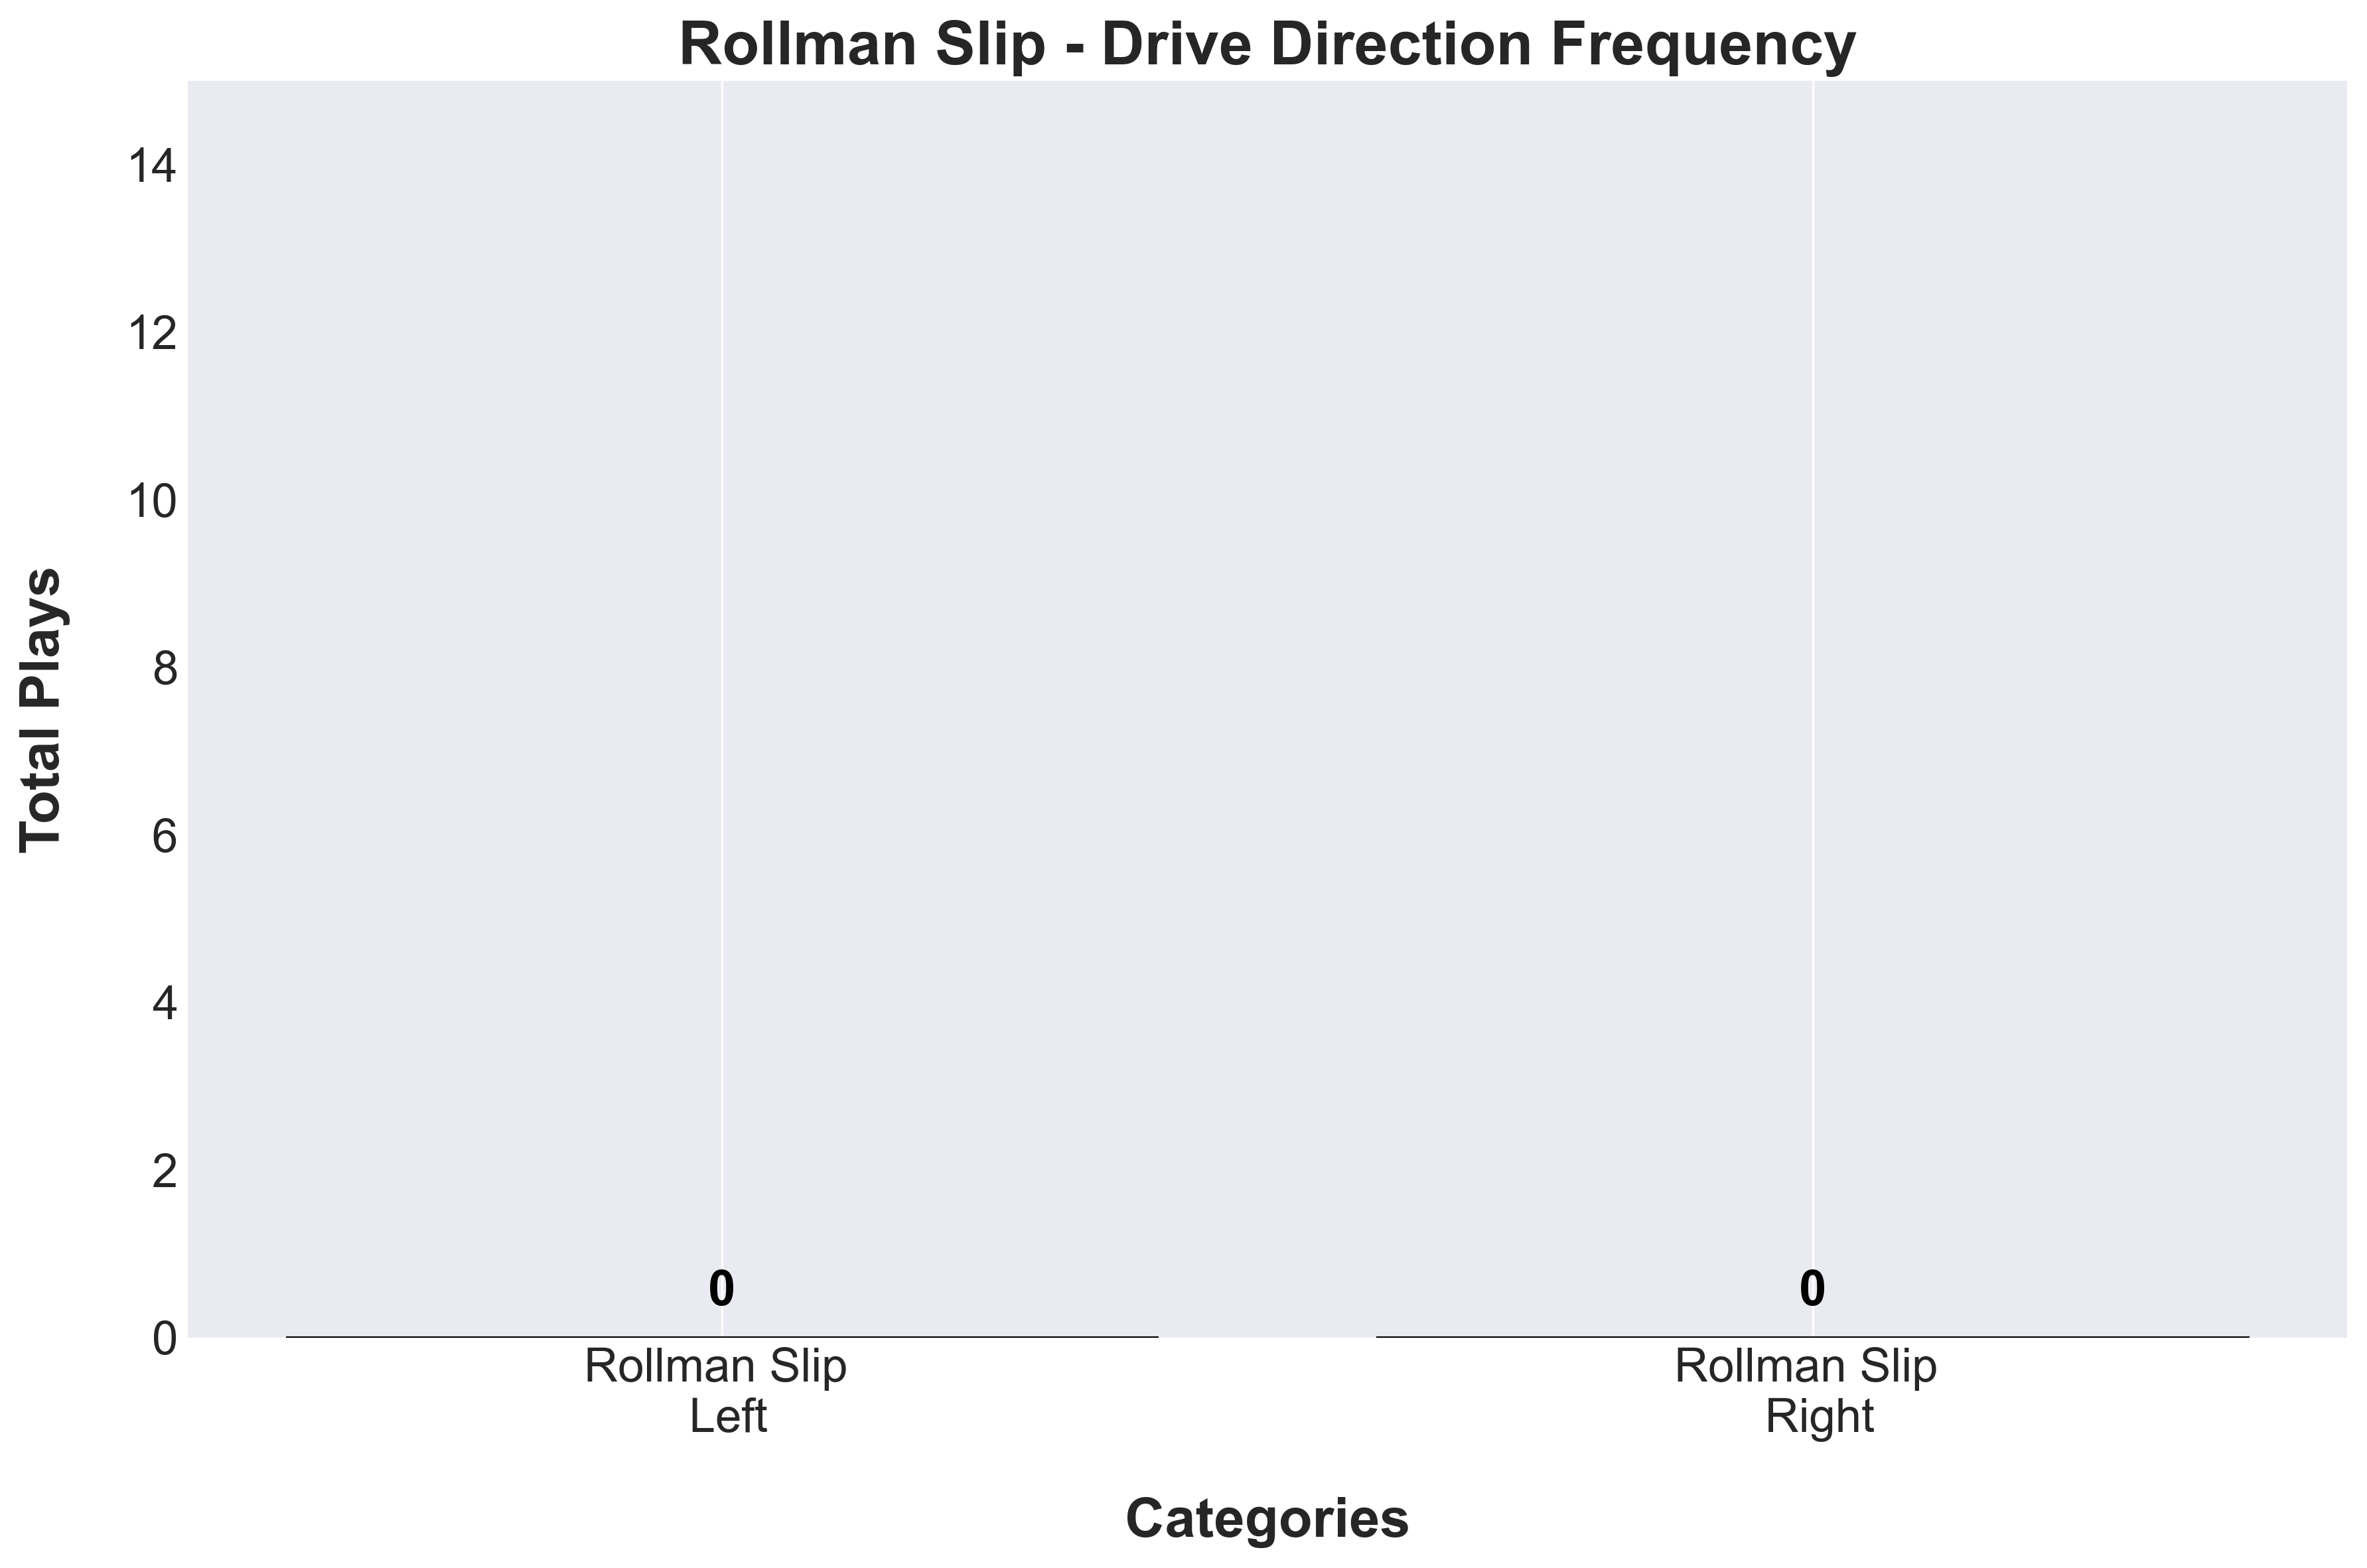
\includegraphics[width=\textwidth, height=.14\textheight]{images/Rollman_SlipDirection_Freq.png} % Adjust the width of the image to fit
    \end{minipage}
    
\end{table}

\vspace{-1em} % Add vertical space before the line (optional)
%\hrule height 1pt width 1\textwidth % Adjust height and width
\vspace{-1em} % Add vertical space after the line (optional)

% Rollman Pop Drive Direction
\begin{table}[H]
    \raisebox{3.5em}{ % Adjust this value to shift the tables vertically
    \begin{minipage}[t]{0.6\textwidth} % Left side (table) takes 85% of the width
        \flushleft
        \centering % Centering the title and the table
        \text{Rollman Pop to Drive Direction Statistics} % Title above the table in bold
        \vskip .25em % Adds vertical space between title and table
        \scalebox{.6}{ % Scale the entire table down by half
            \renewcommand{\arraystretch}{1.4} % Adjust the number to increase or decrease row spacing
            \begin{tabular}{
            >{\centering\arraybackslash}p{1.75cm} 
            >{\centering\arraybackslash}p{.75cm} 
            >{\centering\arraybackslash}p{.75cm} 
            >{\centering\arraybackslash}p{.75cm} 
            >{\centering\arraybackslash}p{.75cm}
            >{\centering\arraybackslash}p{.75cm} 
            >{\centering\arraybackslash}p{.75cm} 
            >{\centering\arraybackslash}p{.75cm} 
            >{\centering\arraybackslash}p{.75cm}
            >{\centering\arraybackslash}p{.75cm} 
            >{\centering\arraybackslash}p{.75cm}
            >{\centering\arraybackslash}p{.75cm}
            >{\centering\arraybackslash}p{.75cm} 
            >{\centering\arraybackslash}p{.75cm}}% Adjust column widths
            \toprule
            {\scriptsize \textbf{PlayType}} &
            {\scriptsize \textbf{Plays}} &
            {\scriptsize \textbf{3PA}} &
            {\scriptsize \textbf{3PM}} &
            {\scriptsize \textbf{3P\%}} & 
            {\scriptsize \textbf{2PA}} & 
            {\scriptsize \textbf{2PM}} & 
            {\scriptsize \textbf{2P\%}} & 
            {\scriptsize \textbf{MiA}} & 
            {\scriptsize \textbf{MiM}} &
            {\scriptsize \textbf{Mi\%}} &
            {\scriptsize \textbf{EFG\%}} &
            {\scriptsize \textbf{TO}} &
            {\scriptsize \textbf{Foul}} \\
            \midrule
            
                
            
                
            
                
            
                
            
                
            
                
            
                
            
                
            
                
            
                
            
                
            
                
            
                
            
                
            
                
            
                
            


            \bottomrule
        \end{tabular}
        } % End of \scalebox
    \end{minipage}
    } % End of raisebox, closing the adjustment
    \hfill
    \begin{minipage}[c]{0.35\textwidth} % Right side (image) takes 10% of the width
        \flushright
        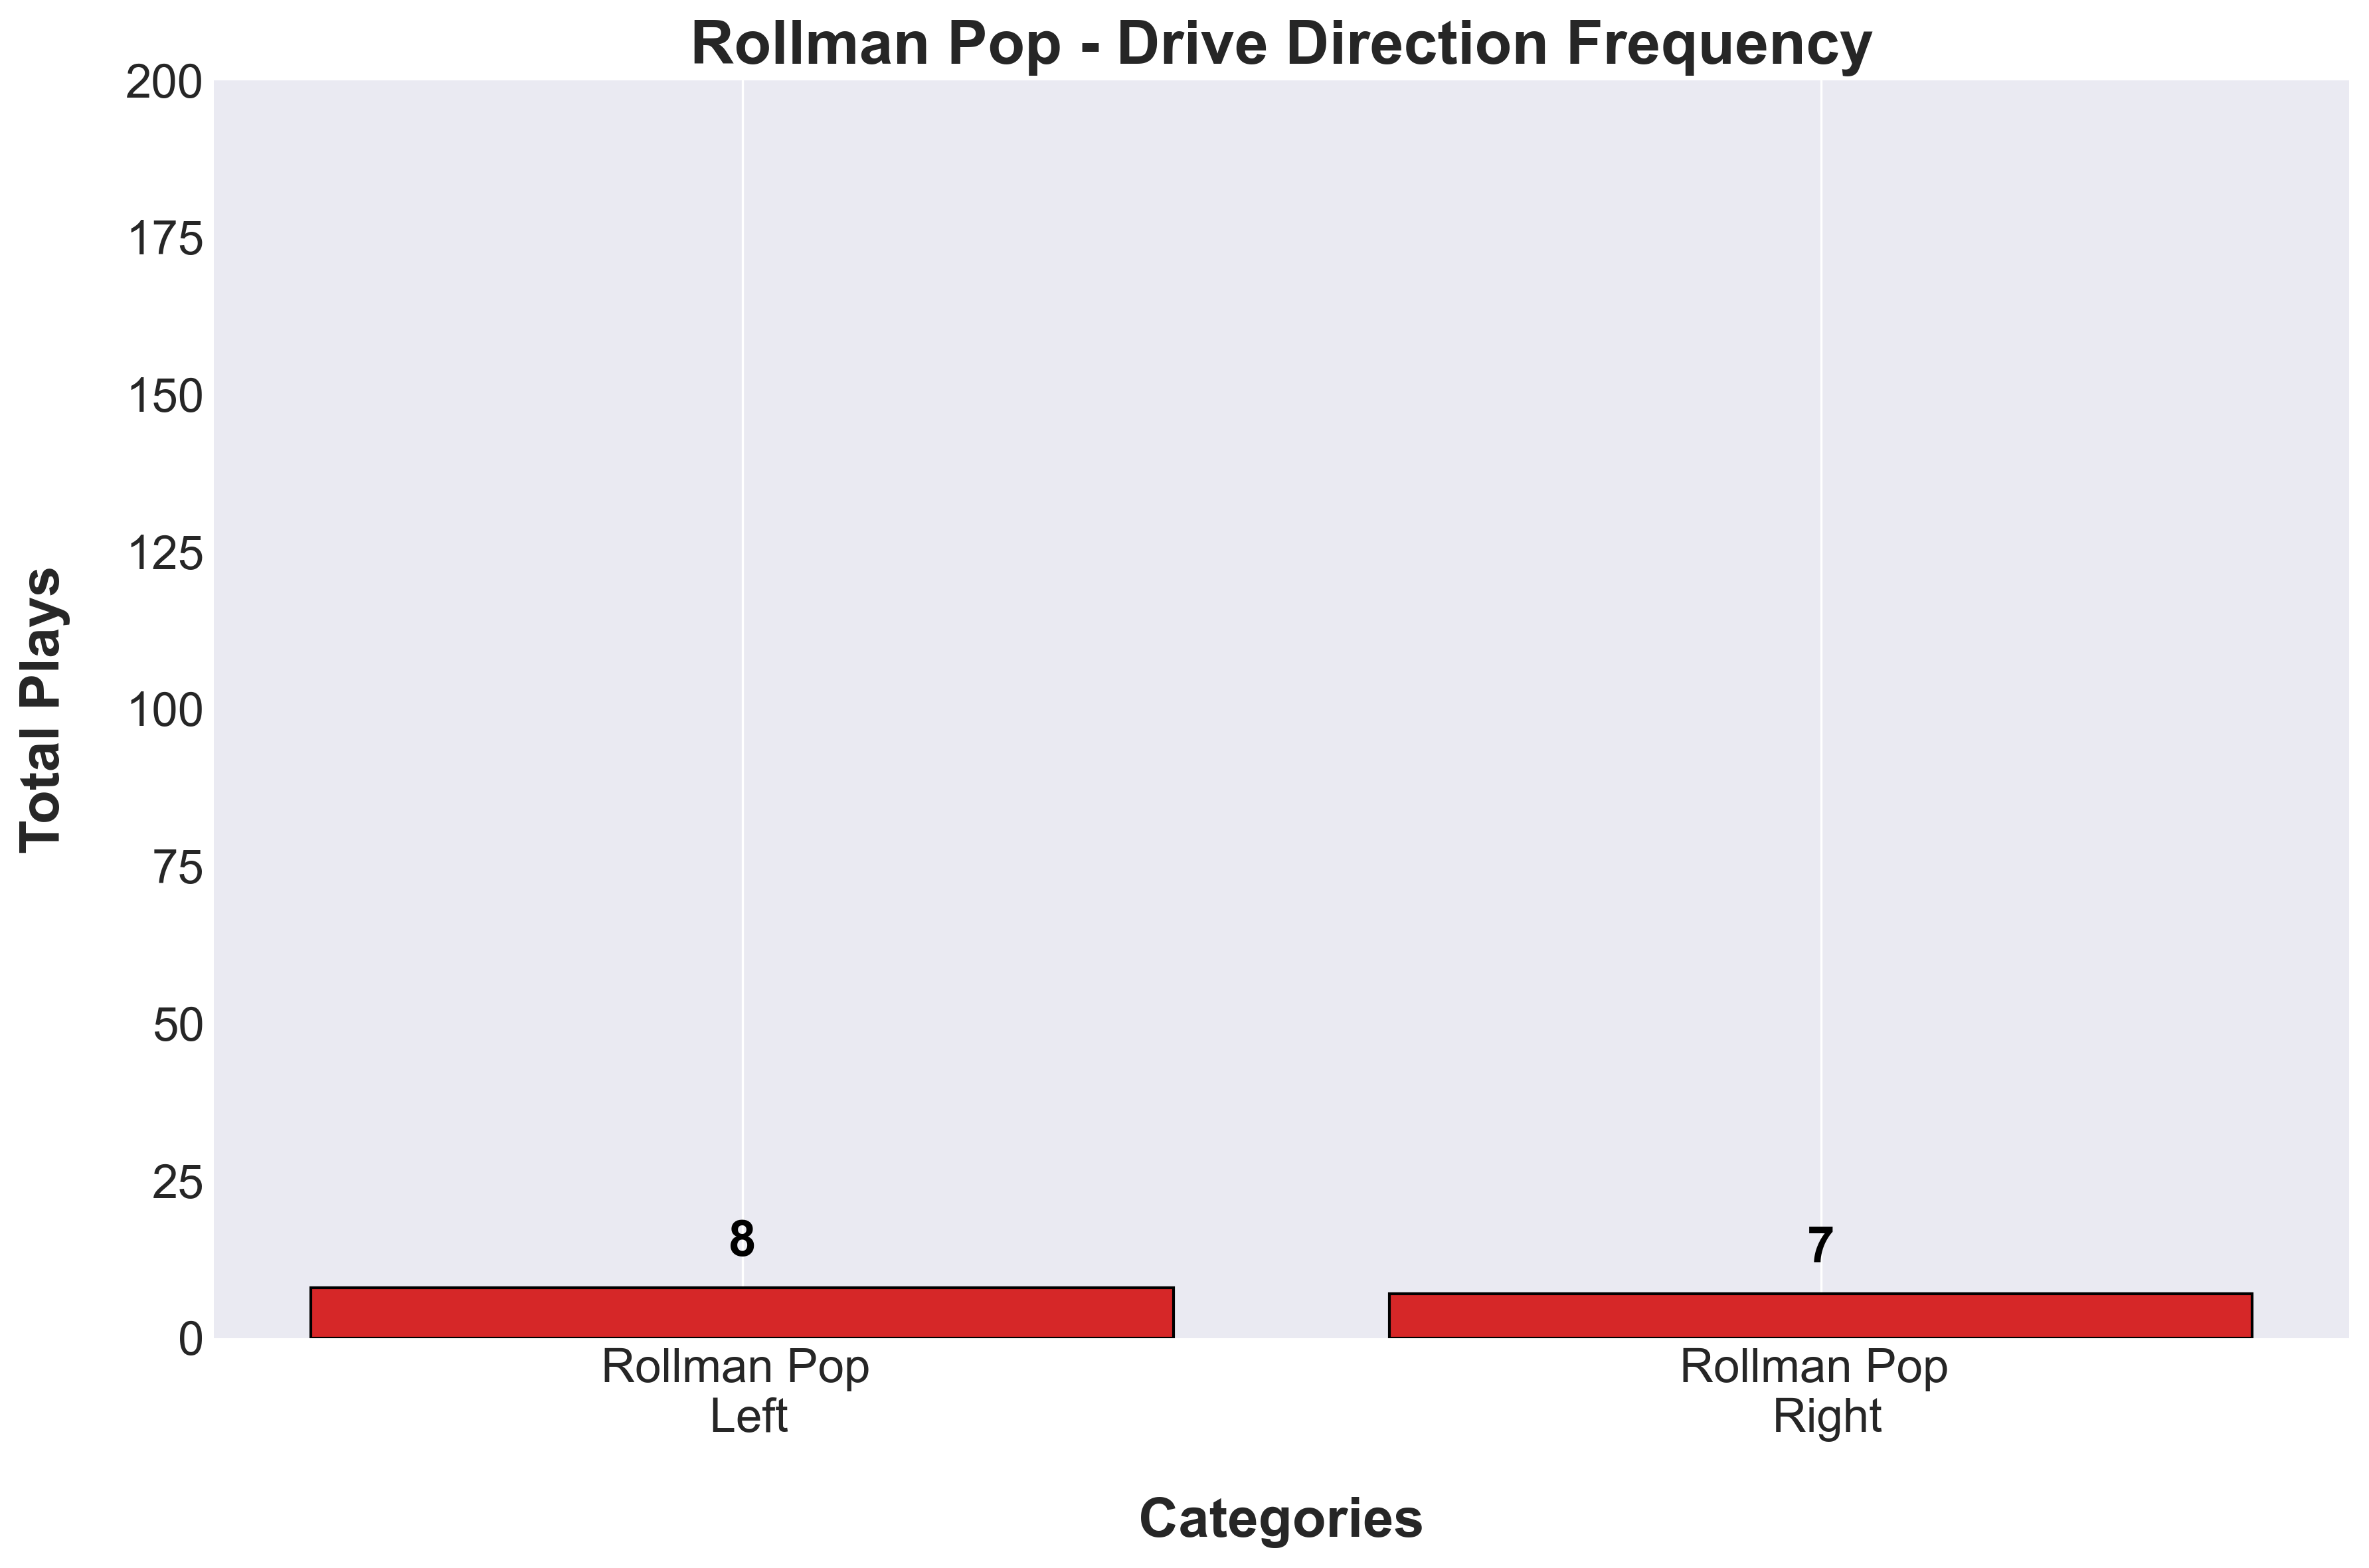
\includegraphics[width=\textwidth, height=.14\textheight]{images/Rollman_PopDirection_Freq.png} % Adjust the width of the image to fit
    \end{minipage}
    
\end{table}

\vspace{-1em} % Add vertical space before the line (optional)
\hrule height 1pt width 1\textwidth % Adjust height and width
\vspace{1em} % Add vertical space after the line (optional)

\subsubsection{Rollman by Passer Statistics}

\vspace{-1em} % Add vertical space before the line (optional)

% Rollman Slips Stats by Passer
\begin{table}[H]
    \raisebox{3em}{ % Adjust this value to shift the tables vertically
    \begin{minipage}[t]{0.6\textwidth} % Left side (table) takes 85% of the width
        \flushleft
        \centering % Centering the title and the table
        \text{Rollman Slip Stats by Passer} % Title above the table in bold
        \vskip .25em % Adds vertical space between title and table
        \scalebox{.55}{ % Scale the entire table down by half
            \renewcommand{\arraystretch}{1.4} % Adjust the number to increase or decrease row spacing
            \begin{tabular}{
            >{\centering\arraybackslash}p{3cm} 
            >{\centering\arraybackslash}p{.75cm} 
            >{\centering\arraybackslash}p{.75cm} 
            >{\centering\arraybackslash}p{.75cm} 
            >{\centering\arraybackslash}p{.75cm}
            >{\centering\arraybackslash}p{.75cm} 
            >{\centering\arraybackslash}p{.75cm} 
            >{\centering\arraybackslash}p{.75cm} 
            >{\centering\arraybackslash}p{.75cm}
            >{\centering\arraybackslash}p{.75cm} 
            >{\centering\arraybackslash}p{.75cm}
            >{\centering\arraybackslash}p{.75cm}
            >{\centering\arraybackslash}p{.75cm} 
            >{\centering\arraybackslash}p{.75cm}}% Adjust column widths
            \toprule
            {\scriptsize \textbf{Player}} &
            {\scriptsize \textbf{Plays}} &
            {\scriptsize \textbf{3PA}} &
            {\scriptsize \textbf{3PM}} &
            {\scriptsize \textbf{3P\%}} & 
            {\scriptsize \textbf{2PA}} & 
            {\scriptsize \textbf{2PM}} & 
            {\scriptsize \textbf{2P\%}} & 
            {\scriptsize \textbf{MiA}} & 
            {\scriptsize \textbf{MiM}} &
            {\scriptsize \textbf{Mi\%}} &
            {\scriptsize \textbf{EFG\%}} &
            {\scriptsize \textbf{TO}} &
            {\scriptsize \textbf{Foul}} \\
            \midrule
            
                
            
                
            
                
            
                
            
                
            
                
            
                
            
                
            
                
            
                
            
                
            
                
            
                
            
                
                    
                
            
                
            
                
            

            \bottomrule
        \end{tabular}
        } % End of \scalebox
    \end{minipage}
    } % End of raisebox, closing the adjustment
    \hfill % This adds some flexible space between the table and the image
    \begin{minipage}[c]{0.35\textwidth} % Right side (image) takes 10% of the width
        \flushright
        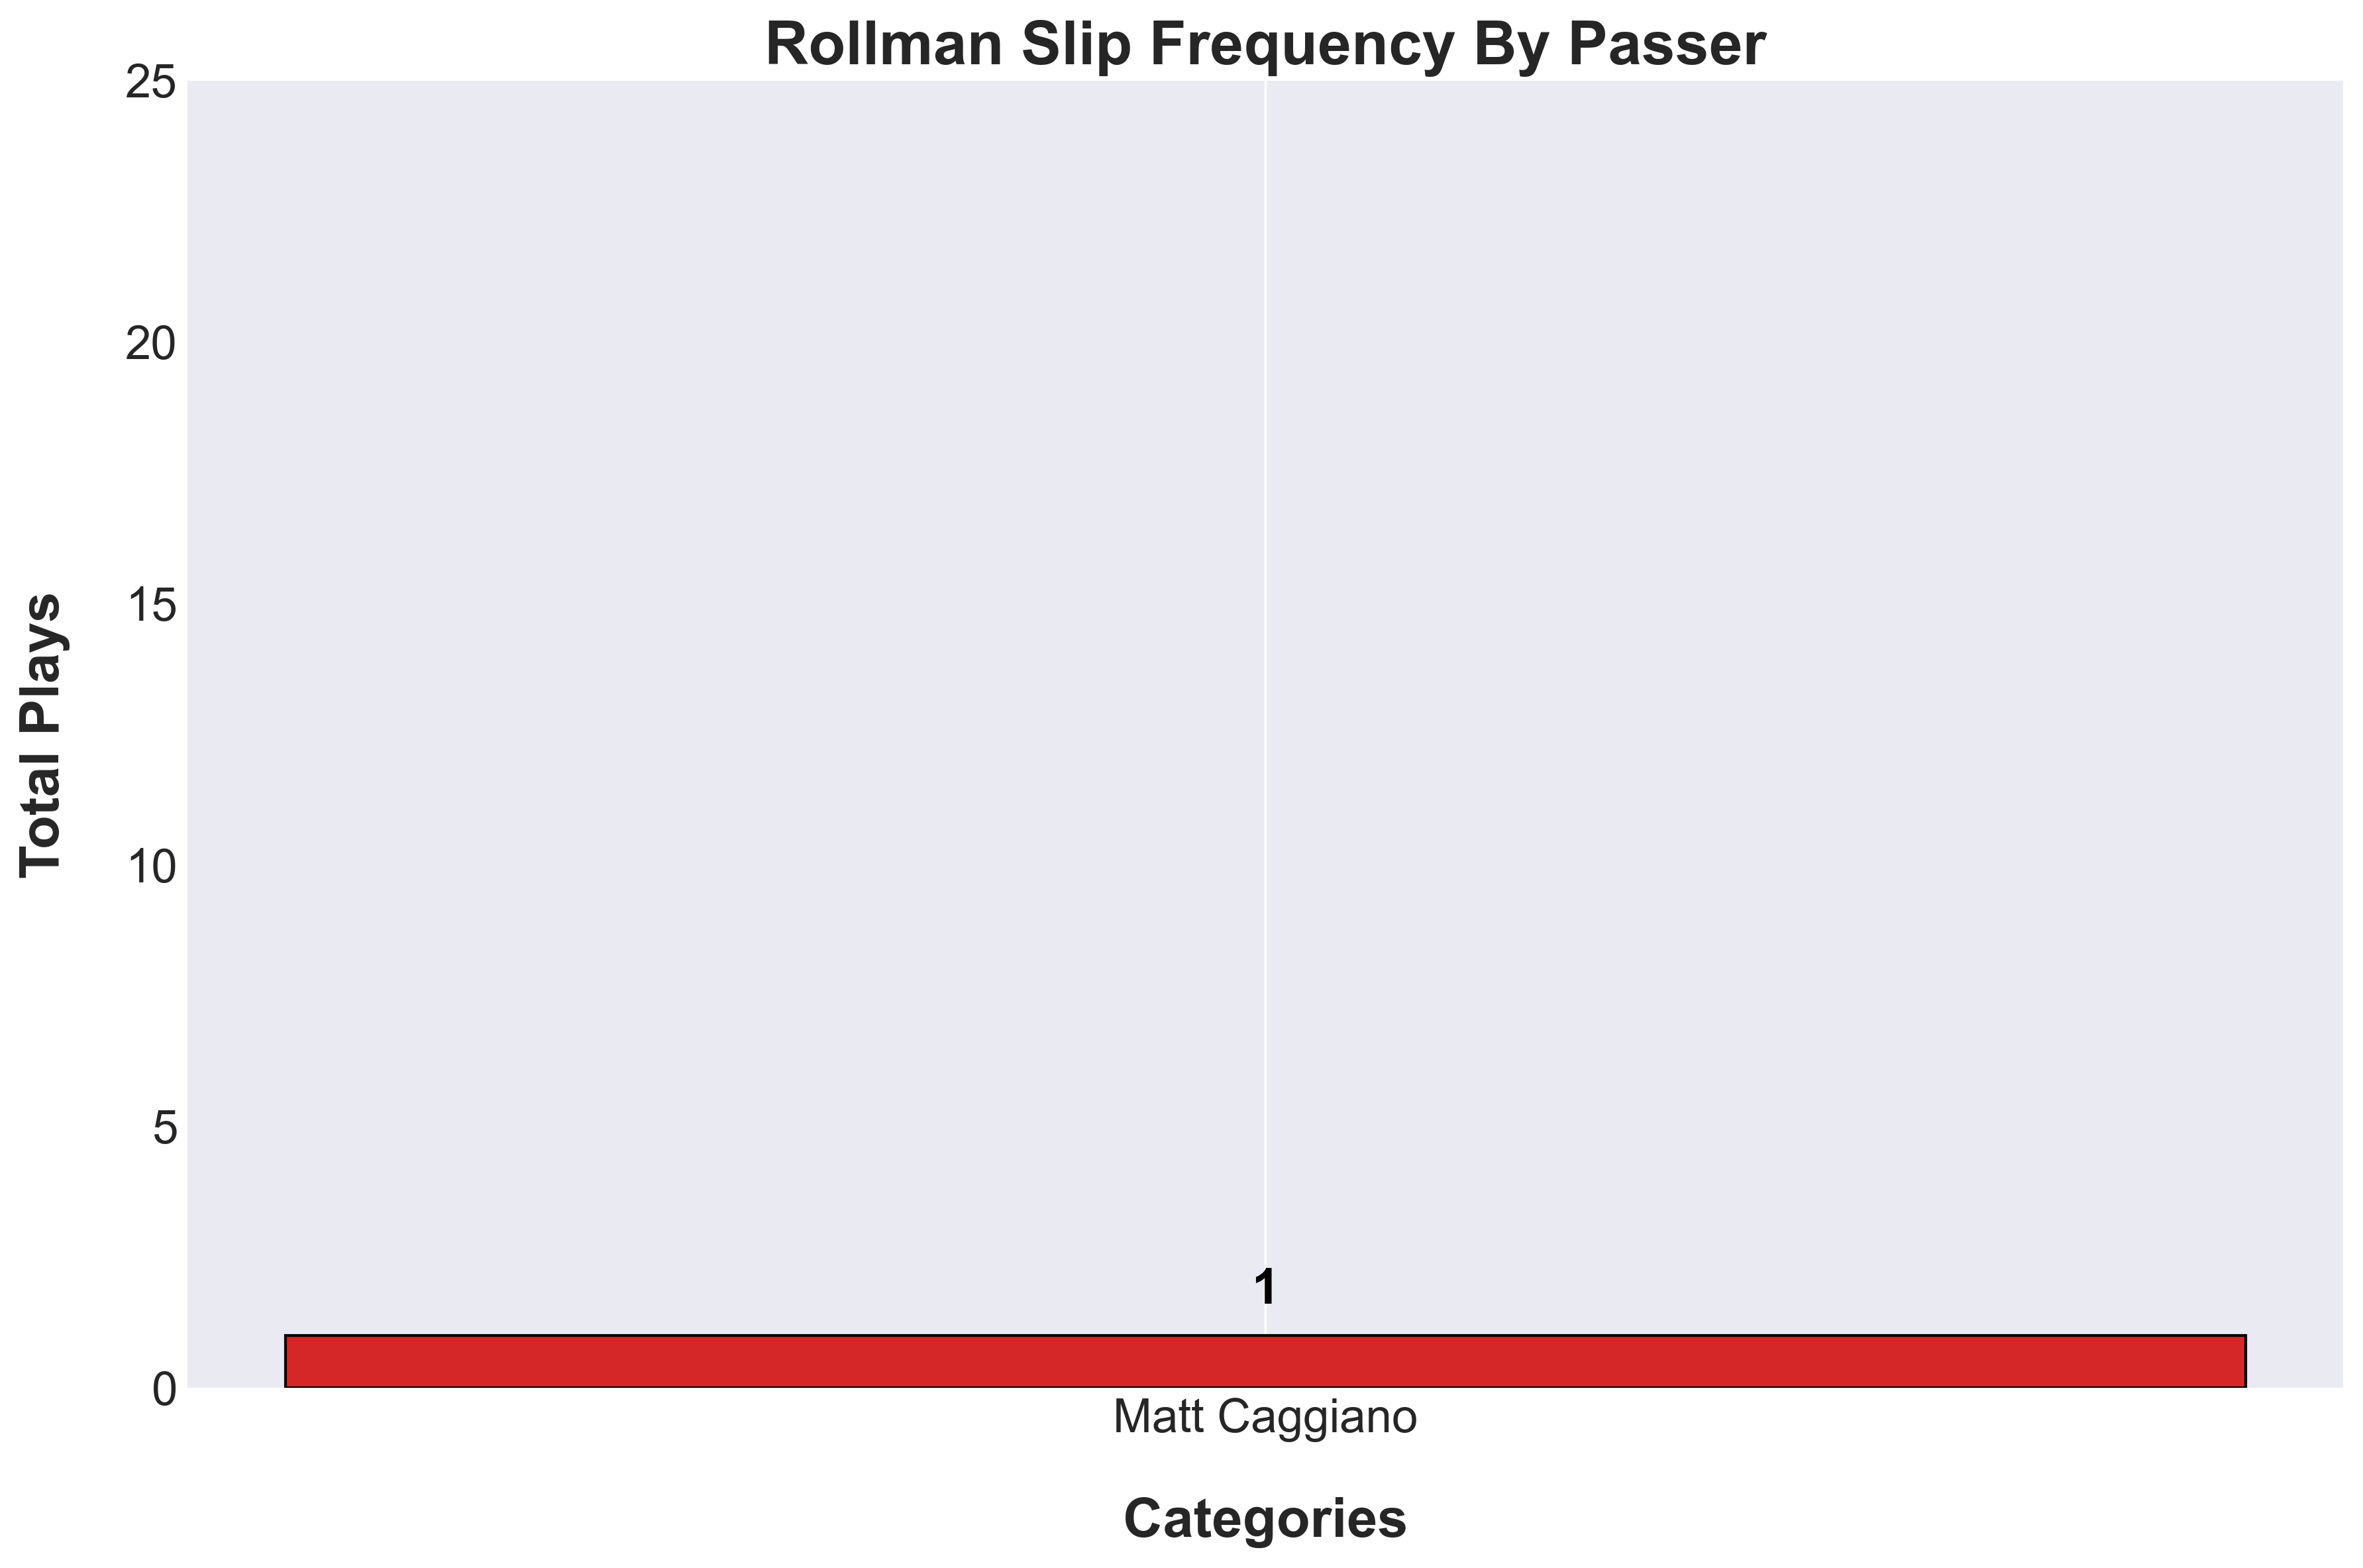
\includegraphics[width=\textwidth, height=.14\textheight]{images/Rollman_SlipPlayer_Freq.png} % Adjust the width of the image to fit
    \end{minipage}
\end{table}

\vspace{-1em} % Add vertical space before the line (optional)
\vspace{-1em} % Add vertical space after the line (optional)

% Rollman Pop Stats by Passer
\begin{table}[H]
    \raisebox{3em}{ % Adjust this value to shift the tables vertically
    \begin{minipage}[t]{0.6\textwidth} % Left side (table) takes 85% of the width
        \flushleft
        \centering % Centering the title and the table
        \text{Rollman Pop Stats by Passer} % Title above the table in bold
        \vskip .25em % Adds vertical space between title and table
        \scalebox{.55}{ % Scale the entire table down by half
            \renewcommand{\arraystretch}{1.4} % Adjust the number to increase or decrease row spacing
            \begin{tabular}{
            >{\centering\arraybackslash}p{3cm} 
            >{\centering\arraybackslash}p{.75cm} 
            >{\centering\arraybackslash}p{.75cm} 
            >{\centering\arraybackslash}p{.75cm} 
            >{\centering\arraybackslash}p{.75cm}
            >{\centering\arraybackslash}p{.75cm} 
            >{\centering\arraybackslash}p{.75cm} 
            >{\centering\arraybackslash}p{.75cm} 
            >{\centering\arraybackslash}p{.75cm}
            >{\centering\arraybackslash}p{.75cm} 
            >{\centering\arraybackslash}p{.75cm}
            >{\centering\arraybackslash}p{.75cm}
            >{\centering\arraybackslash}p{.75cm} 
            >{\centering\arraybackslash}p{.75cm}}% Adjust column widths
            \toprule
            {\scriptsize \textbf{Player}} &
            {\scriptsize \textbf{Plays}} &
            {\scriptsize \textbf{3PA}} &
            {\scriptsize \textbf{3PM}} &
            {\scriptsize \textbf{3P\%}} & 
            {\scriptsize \textbf{2PA}} & 
            {\scriptsize \textbf{2PM}} & 
            {\scriptsize \textbf{2P\%}} & 
            {\scriptsize \textbf{MiA}} & 
            {\scriptsize \textbf{MiM}} &
            {\scriptsize \textbf{Mi\%}} &
            {\scriptsize \textbf{EFG\%}} &
            {\scriptsize \textbf{TO}} &
            {\scriptsize \textbf{Foul}} \\
            \midrule
            
                
            
                
            
                
            
                
            
                
            
                
            
                
            
                
            
                
            
                
            
                
            
                
            
                
            
                
            
                
                    
                
            
                
            

            \bottomrule
        \end{tabular}
        } % End of \scalebox
    \end{minipage}
    } % End of raisebox, closing the adjustment
    \hfill % This adds some flexible space between the table and the image
    \begin{minipage}[c]{0.35\textwidth} % Right side (image) takes 10% of the width
        \flushright
        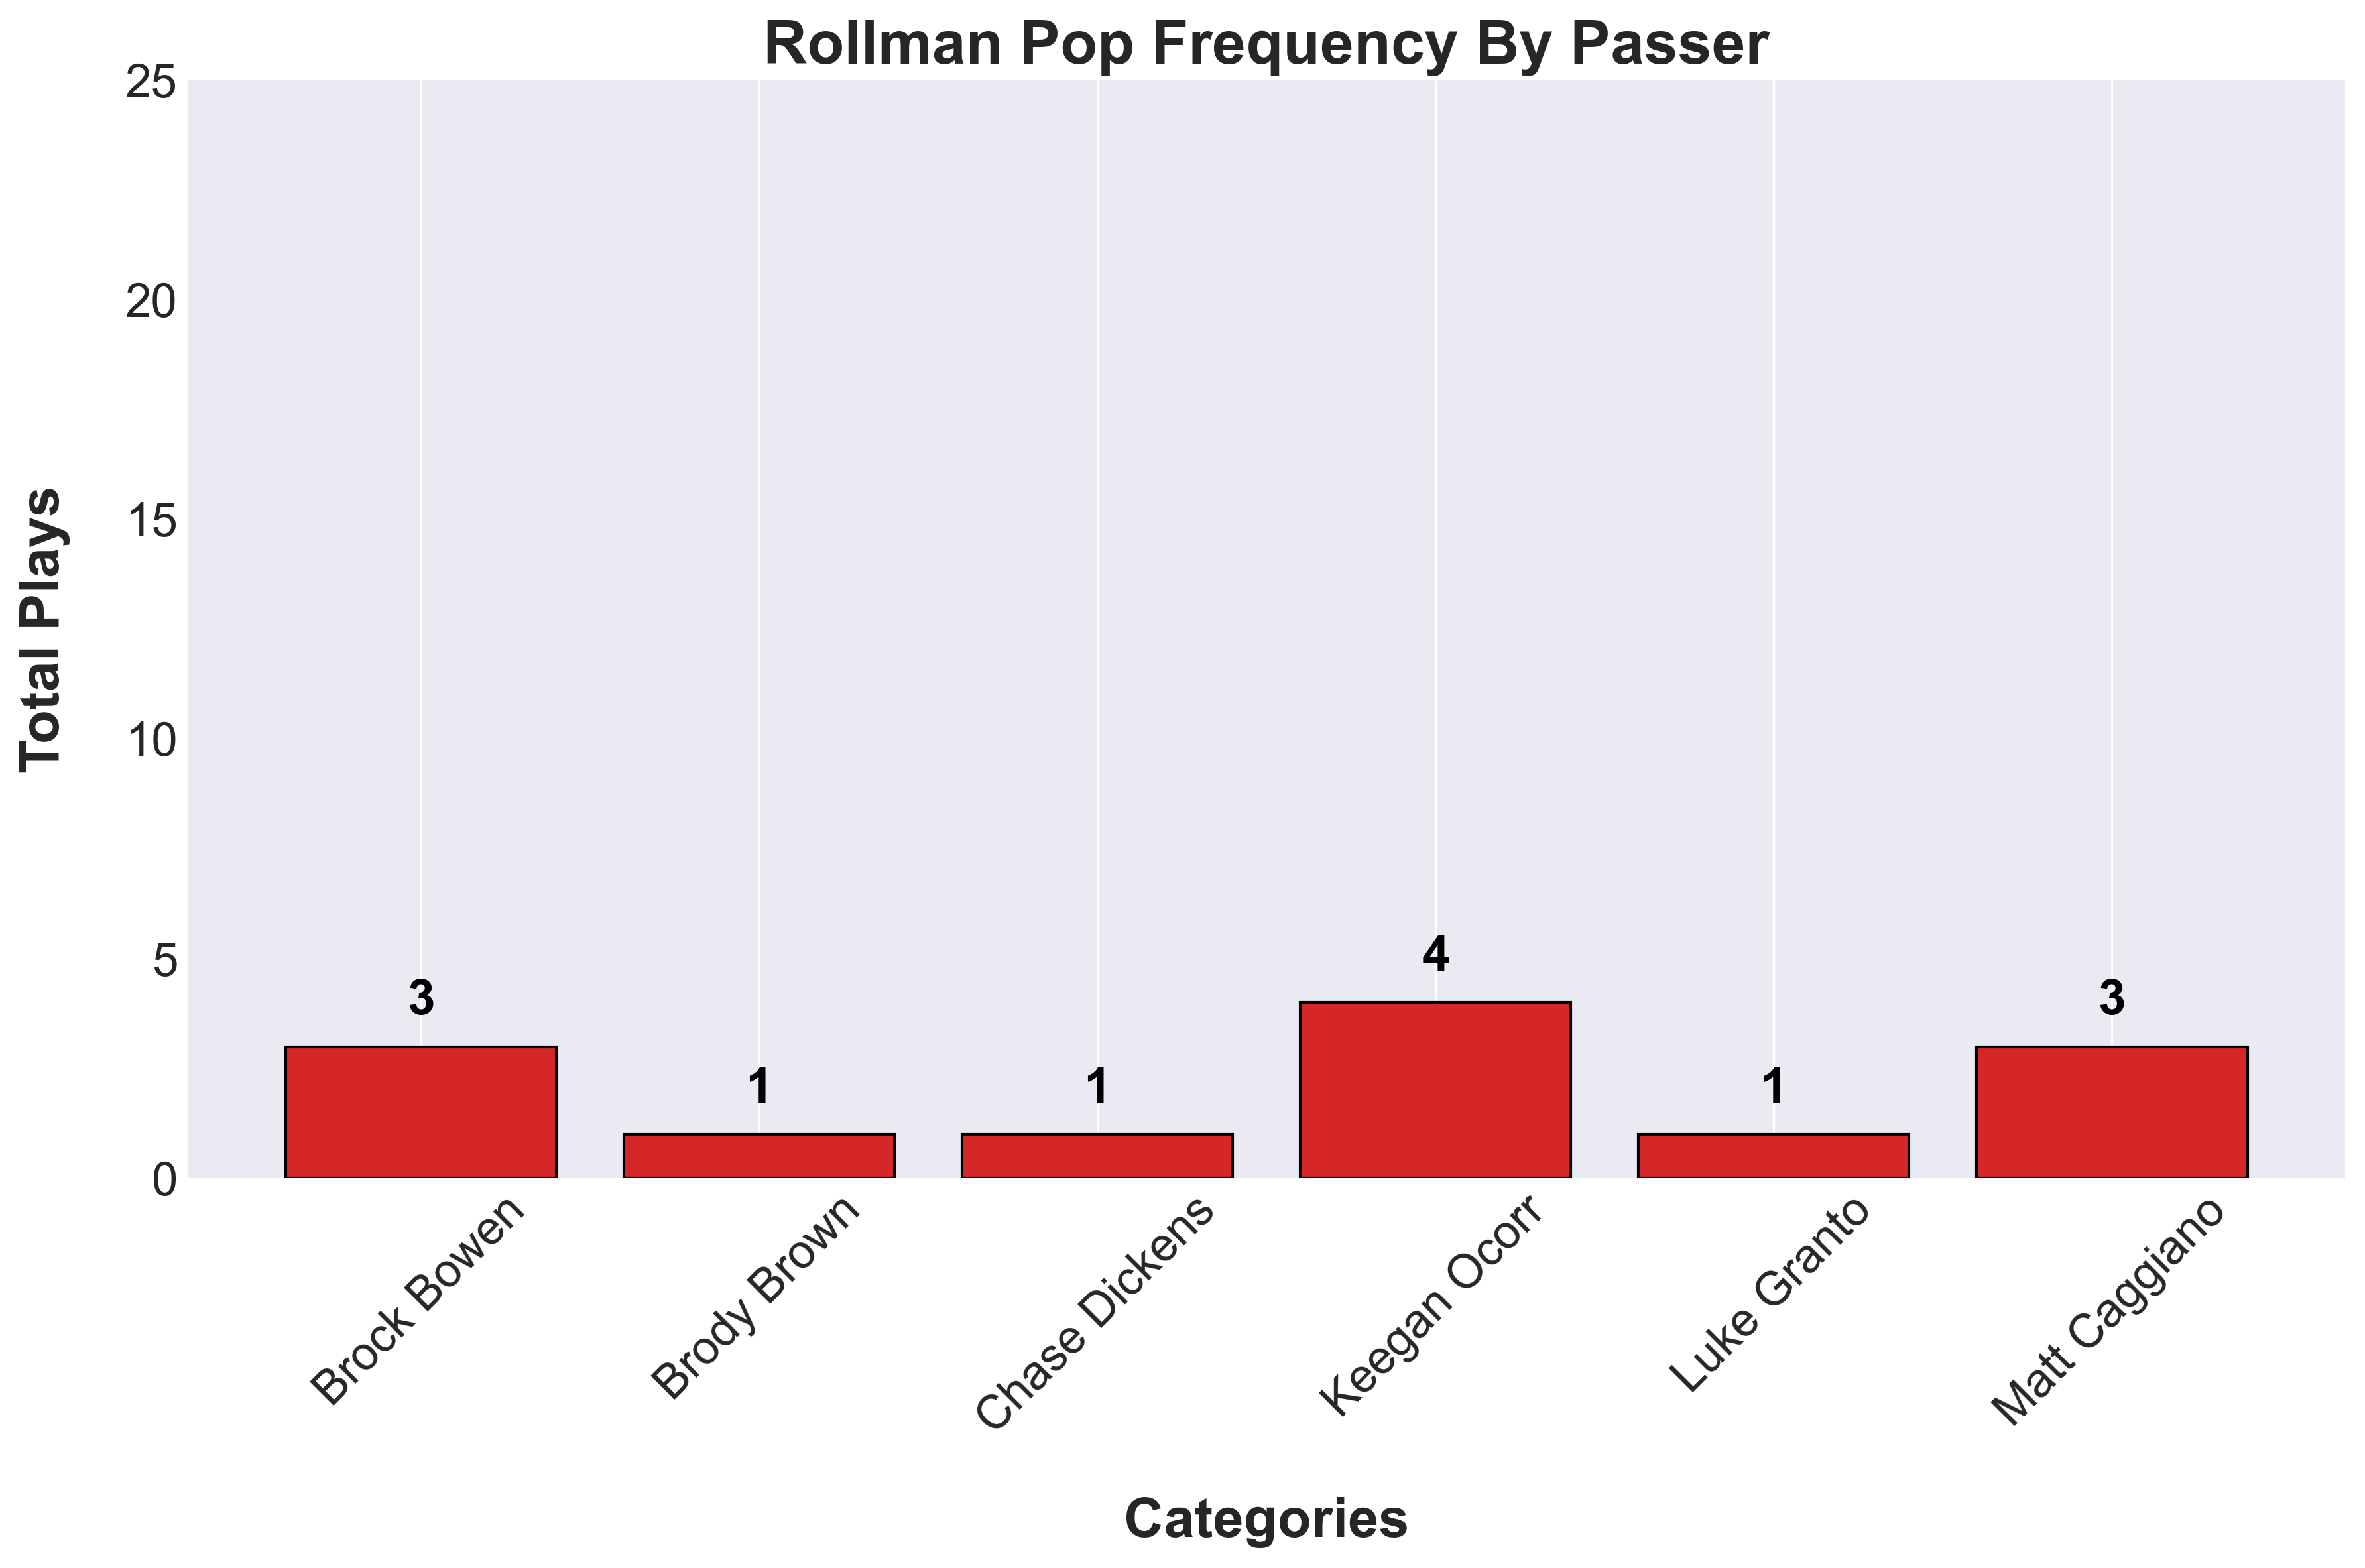
\includegraphics[width=\textwidth, height=.14\textheight]{images/Rollman_PopPlayer_Freq.png} % Adjust the width of the image to fit
    \end{minipage}
\end{table}

\vspace{-1em} % Add vertical space before the line (optional)
\vspace{-1em} % Add vertical space after the line (optional)

% Rollman Rolls Stats by Passer
\begin{table}[H]
    \raisebox{3em}{ % Adjust this value to shift the tables vertically
    \begin{minipage}[t]{0.6\textwidth} % Left side (table) takes 85% of the width
        \flushleft
        \centering % Centering the title and the table
        \text{Rollman Roll Stats by Passer} % Title above the table in bold
        \vskip .25em % Adds vertical space between title and table
        \scalebox{.55}{ % Scale the entire table down by half
            \renewcommand{\arraystretch}{1.4} % Adjust the number to increase or decrease row spacing
            \begin{tabular}{
            >{\centering\arraybackslash}p{3cm} 
            >{\centering\arraybackslash}p{.75cm} 
            >{\centering\arraybackslash}p{.75cm} 
            >{\centering\arraybackslash}p{.75cm} 
            >{\centering\arraybackslash}p{.75cm}
            >{\centering\arraybackslash}p{.75cm} 
            >{\centering\arraybackslash}p{.75cm} 
            >{\centering\arraybackslash}p{.75cm} 
            >{\centering\arraybackslash}p{.75cm}
            >{\centering\arraybackslash}p{.75cm} 
            >{\centering\arraybackslash}p{.75cm}
            >{\centering\arraybackslash}p{.75cm}
            >{\centering\arraybackslash}p{.75cm} 
            >{\centering\arraybackslash}p{.75cm}}% Adjust column widths
            \toprule
            {\scriptsize \textbf{Player}} &
            {\scriptsize \textbf{Plays}} &
            {\scriptsize \textbf{3PA}} &
            {\scriptsize \textbf{3PM}} &
            {\scriptsize \textbf{3P\%}} & 
            {\scriptsize \textbf{2PA}} & 
            {\scriptsize \textbf{2PM}} & 
            {\scriptsize \textbf{2P\%}} & 
            {\scriptsize \textbf{MiA}} & 
            {\scriptsize \textbf{MiM}} &
            {\scriptsize \textbf{Mi\%}} &
            {\scriptsize \textbf{EFG\%}} &
            {\scriptsize \textbf{TO}} &
            {\scriptsize \textbf{Foul}} \\
            \midrule
            
                
            
                
            
                
            
                
            
                
            
                
            
                
            
                
            
                
            
                
            
                
            
                
            
                
            
                
            
                
            
                
                    
                
            

            \bottomrule
        \end{tabular}
        } % End of \scalebox
    \end{minipage}
    } % End of raisebox, closing the adjustment
    \hfill % This adds some flexible space between the table and the image
    \begin{minipage}[c]{0.35\textwidth} % Right side (image) takes 10% of the width
        \flushright
        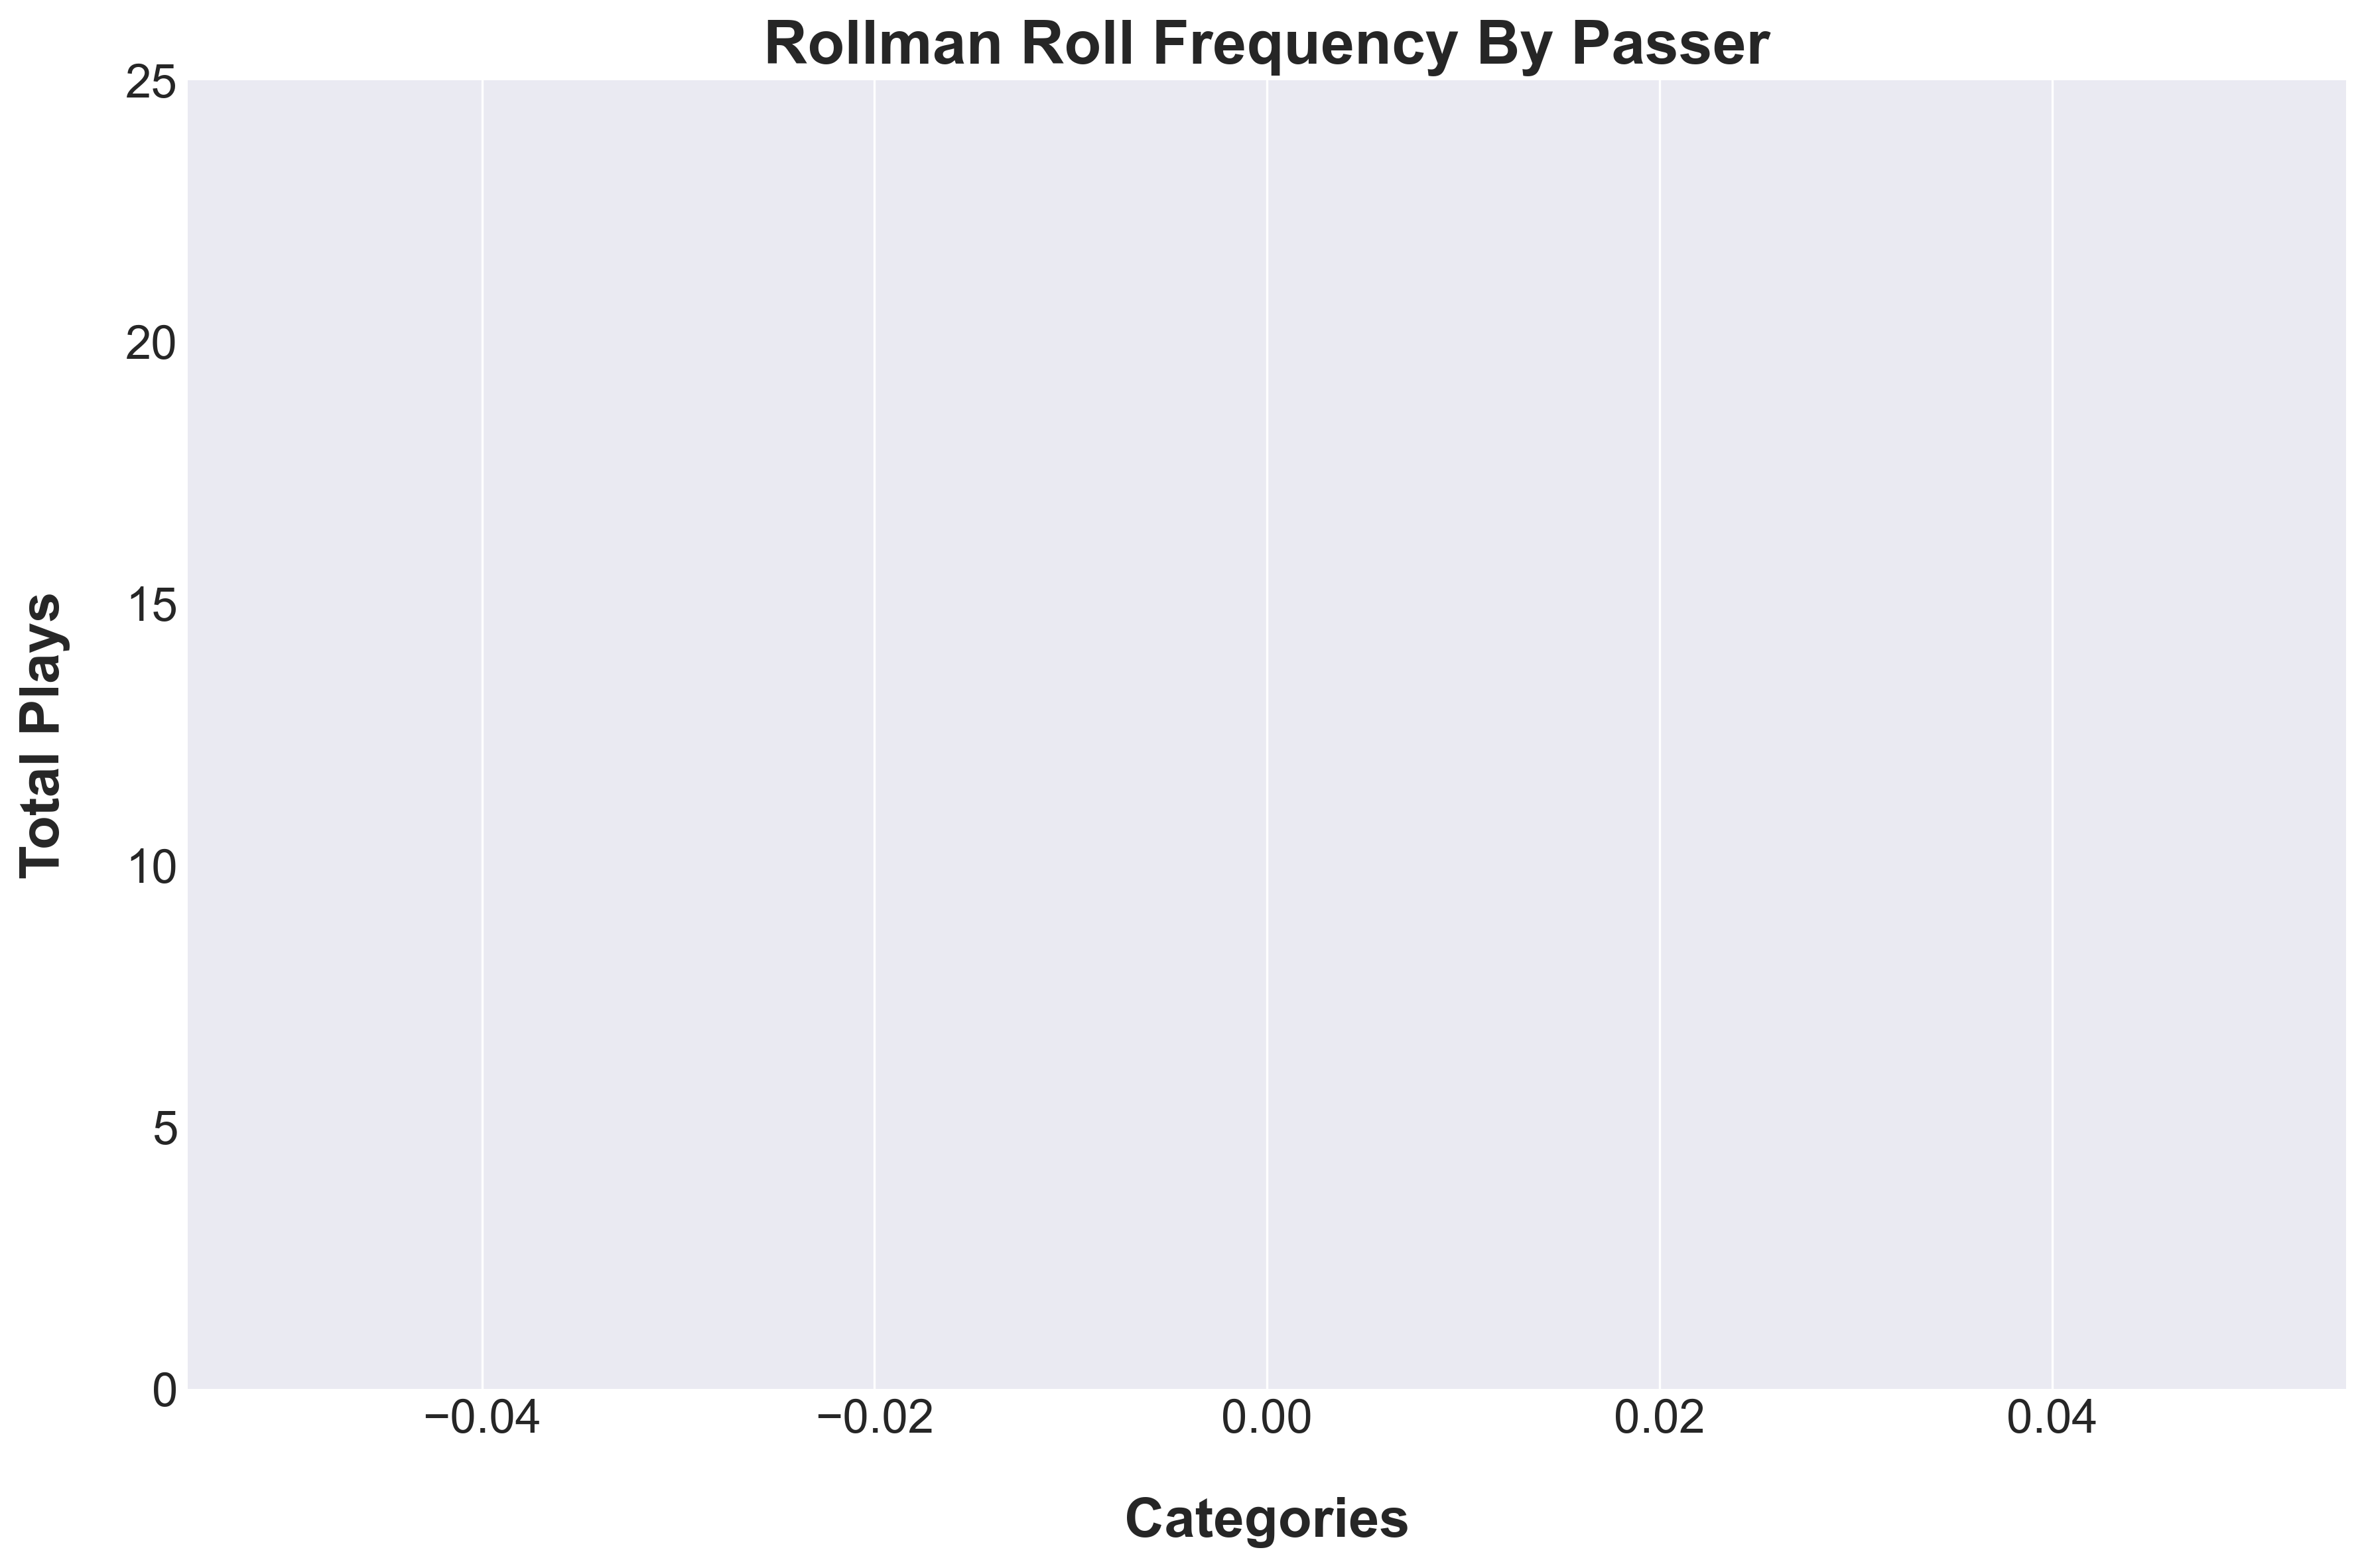
\includegraphics[width=\textwidth, height=.14\textheight]{images/Rollman_RollPlayer_Freq.png} % Adjust the width of the image to fit
    \end{minipage}
\end{table}

\vspace{-1em} % Add vertical space before the line (optional)
\hrule height 1pt width 1\textwidth % Adjust height and width
\vspace{1em} % Add vertical space after the line (optional)

\clearpage

% ----------------------
% Spot Up Visuals and Insights Section
% ----------------------
\subsection{Spot Ups}

\vspace{1.25em} % Add vertical space before the line (optional)
\textbf{Key Notes on Spot up Tendencies}
\vspace{0.5em} % Add space between the title and the itemized list

\begin{itemize}
    \item Spot up Jumpers/Drives make up x\% of players offensive load
    \vspace{0.3em} % Add space between the title and the itemized list
    \item Player is more likely to drive on Spot up plays with x\% of spotup shots coming off drives
\end{itemize}

\vspace{1em} % Add vertical space before the line (optional)
\hrule height 1pt width 1\textwidth % Adjust height and width
\vspace{0em} % Add vertical space after the line (optional)

\subsubsection{Spot Up Shot / Drive Statistics}

% All Spot up Statistics Table w/ room for insights
\begin{table}[H]
    \centering
    \begin{minipage}[t]{0.6\textwidth} % Left side (table) takes 85% of the width
        %\flushright
        \centering % Centering the title and the table
        \text{Total Spot Up Statistics} % Title above the table in bold
        \vskip .25em % Adds vertical space between title and table
        \scalebox{.85}{ % Scale the entire table down by half
            \scriptsize % Reduce the font size
            \begin{tabular}{
            >{\centering\arraybackslash}p{.75cm} 
            >{\centering\arraybackslash}p{.5cm} 
            >{\centering\arraybackslash}p{.5cm} 
            >{\centering\arraybackslash}p{.5cm}
            >{\centering\arraybackslash}p{.5cm} 
            >{\centering\arraybackslash}p{.5cm} 
            >{\centering\arraybackslash}p{.5cm} 
            >{\centering\arraybackslash}p{.5cm}
            >{\centering\arraybackslash}p{.5cm} 
            >{\centering\arraybackslash}p{.5cm}
            >{\centering\arraybackslash}p{.75cm}
            >{\centering\arraybackslash}p{.5cm} 
            >{\centering\arraybackslash}p{.5cm}}% Adjust column widths
            \toprule
            \textbf{Plays} &
            \textbf{3PA} &
            \textbf{3PM} &
            \textbf{3P\%} & 
            \textbf{2PA} & 
            \textbf{2PM} & 
            \textbf{2P\%} & 
            \textbf{MiA} & 
            \textbf{MiM} &
            \textbf{Mi\%} &
            \textbf{EFG\%} &
            \textbf{TO} &
            \textbf{Foul} \\
            \midrule
            
                
            
                
            
                
            
                
            
                
            
                
            
                
            
                
            
                
            
                
            
                
            
                
            
                
            
                
            
                
            
                
                    79 & 33 & 12 &
                    - & 
                    35 & 20 &
                    - &
                    14 & 7 &
                    - &
                    - &
                    6 & 5 \\
                
            
                
            
                
            
                
            
                
            
                
            
                
            

            \bottomrule
            \end{tabular}
        }
    \end{minipage}
\end{table}

\vspace{0em} % Add vertical space before the line (optional)
%\hrule height 1pt width 1\textwidth % Adjust height and width
\vspace{-1em} % Add vertical space after the line (optional)

% Spot up Stats for Jumpers vs Drives
\begin{table}[H]
    \raisebox{3em}{ % Adjust this value to shift the tables vertically
    \begin{minipage}[t]{0.6\textwidth} % Left side (table) takes 85% of the width
        \flushleft
        \centering % Centering the title and the table
        \text{Spot Up Statistics} % Title above the table in bold
        \vskip .25em % Adds vertical space between title and table
        \scalebox{.6}{ % Scale the entire table down by half
            \renewcommand{\arraystretch}{1.4} % Adjust the number to increase or decrease row spacing
            \begin{tabular}{
            >{\centering\arraybackslash}p{1.75cm} 
            >{\centering\arraybackslash}p{.75cm} 
            >{\centering\arraybackslash}p{.75cm} 
            >{\centering\arraybackslash}p{.75cm} 
            >{\centering\arraybackslash}p{.75cm}
            >{\centering\arraybackslash}p{.75cm} 
            >{\centering\arraybackslash}p{.75cm} 
            >{\centering\arraybackslash}p{.75cm} 
            >{\centering\arraybackslash}p{.75cm}
            >{\centering\arraybackslash}p{.75cm} 
            >{\centering\arraybackslash}p{.75cm}
            >{\centering\arraybackslash}p{.75cm}
            >{\centering\arraybackslash}p{.75cm} 
            >{\centering\arraybackslash}p{.75cm}}% Adjust column widths
            \toprule
            {\scriptsize \textbf{PlayType}} &
            {\scriptsize \textbf{Plays}} &
            {\scriptsize \textbf{3PA}} &
            {\scriptsize \textbf{3PM}} &
            {\scriptsize \textbf{3P\%}} & 
            {\scriptsize \textbf{2PA}} & 
            {\scriptsize \textbf{2PM}} & 
            {\scriptsize \textbf{2P\%}} & 
            {\scriptsize \textbf{MiA}} & 
            {\scriptsize \textbf{MiM}} &
            {\scriptsize \textbf{Mi\%}} &
            {\scriptsize \textbf{EFG\%}} &
            {\scriptsize \textbf{TO}} &
            {\scriptsize \textbf{Foul}} \\
            \midrule
            
                
            
                
            
                
            
                
            
                
            
                
            
                
            
                
            
                
            
                
            
                
            
                
            
                
            
                
            
                
            
                
            
                
            
                
                    Jumpshot & 34 & 33 & 12 &
                    - & 
                    0 & 0 &
                    - &
                    0 & 0 &
                    - &
                    - &
                    0 & 1 \\
                
            
                
                    Drive & 45 & 0 & 0 &
                    - & 
                    35 & 20 &
                    - &
                    14 & 7 &
                    - &
                    - &
                    6 & 4 \\
                
            
                
            
                
            
                
            


            \bottomrule
        \end{tabular}
        } % End of \scalebox
    \end{minipage}
    } % End of raisebox, closing the adjustment
    \hfill % This adds some flexible space between the table and the image
    \begin{minipage}[c]{0.35\textwidth} % Right side (image) takes 10% of the width
        \flushright
        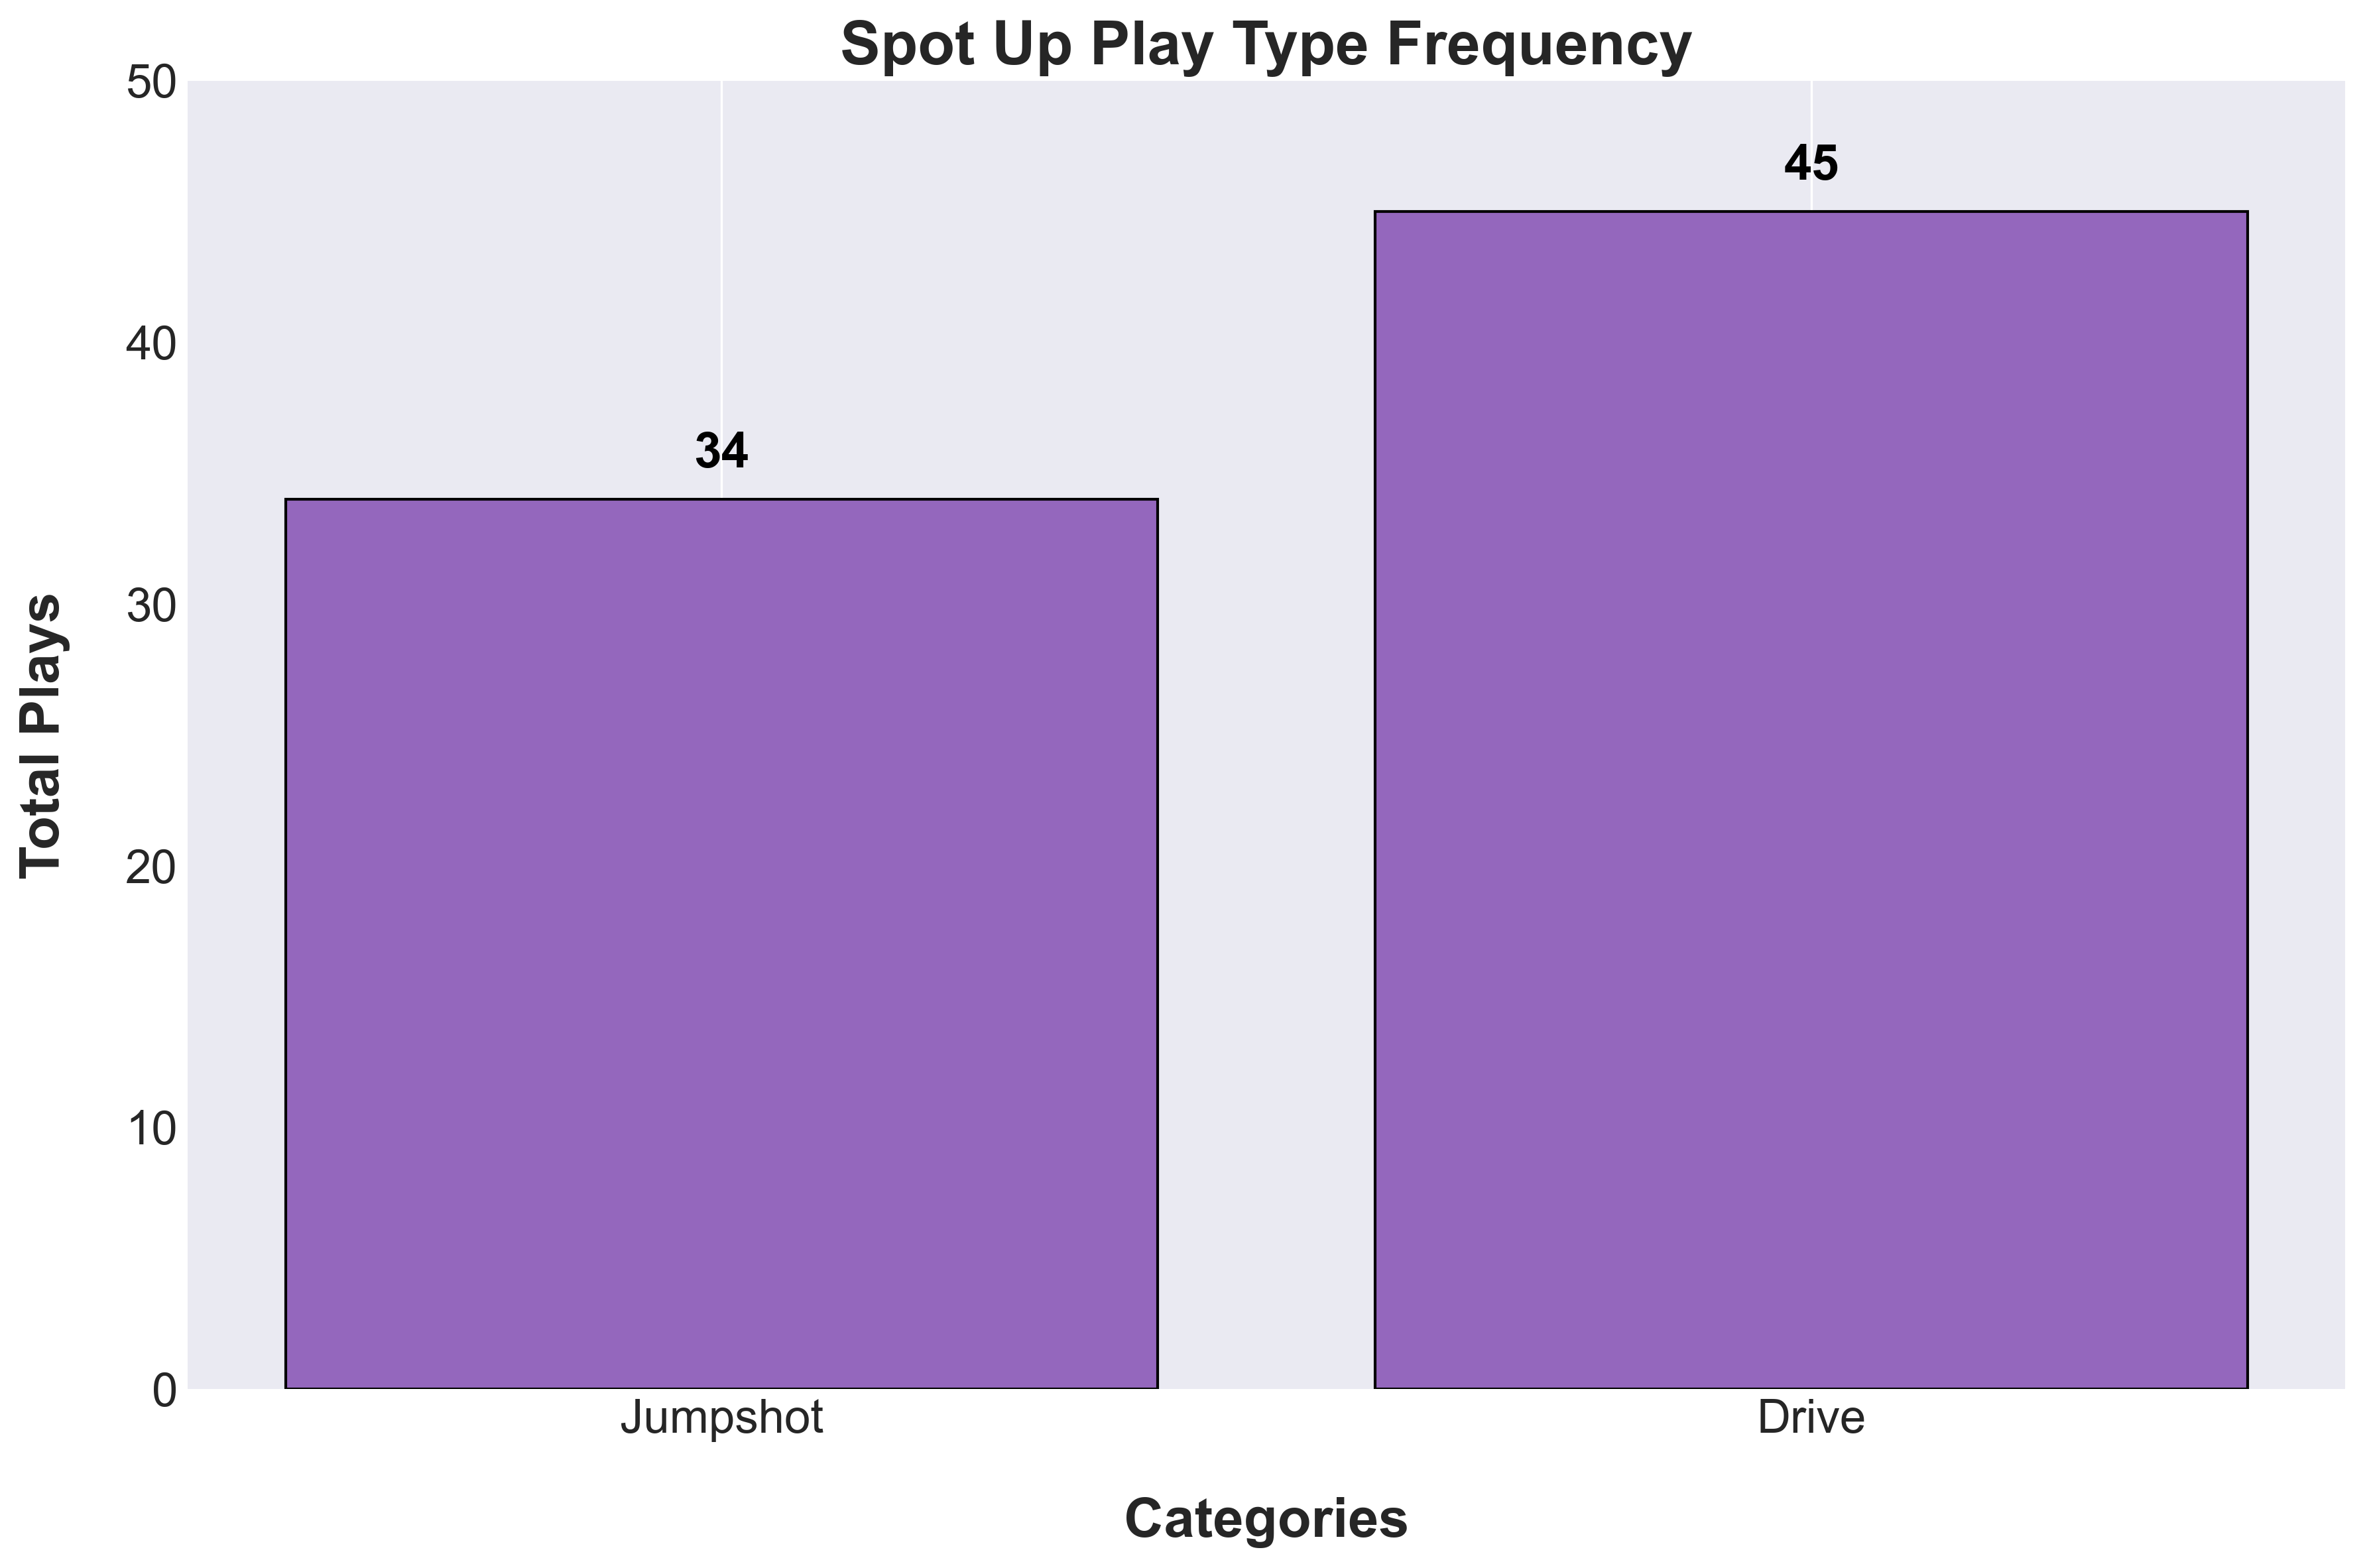
\includegraphics[width=\textwidth, height=.14\textheight]{images/SpotUp_PlayType_Freq.png} % Adjust the width of the image to fit
    \end{minipage}
\end{table}

\vspace{-1em} % Add vertical space before the line (optional)
%\hrule height 1pt width 1\textwidth % Adjust height and width
\vspace{-1em} % Add vertical space after the line (optional)

% Spot up Drives, Left vs Right vs Straight
\begin{table}[H]
    \raisebox{3.5em}{ % Adjust this value to shift the tables vertically
    \centering
    \begin{minipage}[t]{0.6\textwidth} % Left side (table) takes 85% of the width
        \centering % Centering the title and the table
        \text{Drive Direction Statistics} % Title above the table in bold
        \vskip .25em % Adds vertical space between title and table
        \scalebox{.9}{ % Scale the entire table down by half
            \scriptsize % Reduce the font size
            \renewcommand{\arraystretch}{1.4} % Adjust the number to increase or decrease row spacing
            \begin{tabular}{
            >{\centering\arraybackslash}p{1.5cm} 
            >{\centering\arraybackslash}p{.75cm} 
            >{\centering\arraybackslash}p{.5cm} 
            >{\centering\arraybackslash}p{.5cm} 
            >{\centering\arraybackslash}p{.5cm} 
            >{\centering\arraybackslash}p{.5cm}
            >{\centering\arraybackslash}p{.5cm} 
            >{\centering\arraybackslash}p{.5cm}
            >{\centering\arraybackslash}p{.5cm} 
            >{\centering\arraybackslash}p{.5cm}}% Adjust column widths
            \toprule
            \textbf{Direction} & \textbf{Plays} & \textbf{2PA} & \textbf{2PM} & 
            \textbf{2P\%} & \textbf{MiA} & \textbf{MiM} &
            \textbf{Mi\%} & \textbf{TO} & \textbf{Foul} \\
            \midrule
            
                
            
                
            
                
            
                
            
                
            
                
            
                
            
                
            
                
            
                
            
                
            
                
            
                
            
                
            
                
            
                
            
                
            
                
            
                
            
                
                    Left & 21 & 15 & 9 &
                    - &
                    5 & 3 &
                    - &
                    3 & 3 \\
                
            
                
                    Right & 19 & 15 & 10 &
                    - &
                    7 & 3 &
                    - &
                    3 & 1 \\
                
            
                
                    Straight & 5 & 5 & 1 &
                    - &
                    2 & 1 &
                    - &
                    0 & 0 \\
                
            


            \bottomrule
        \end{tabular}
        } % End of \scalebox
    \end{minipage}
    } % End of raisebox, closing the adjustment
    \hfill
    \begin{minipage}[c]{0.35\textwidth} % Right side (image) takes 10% of the width
        \flushright
        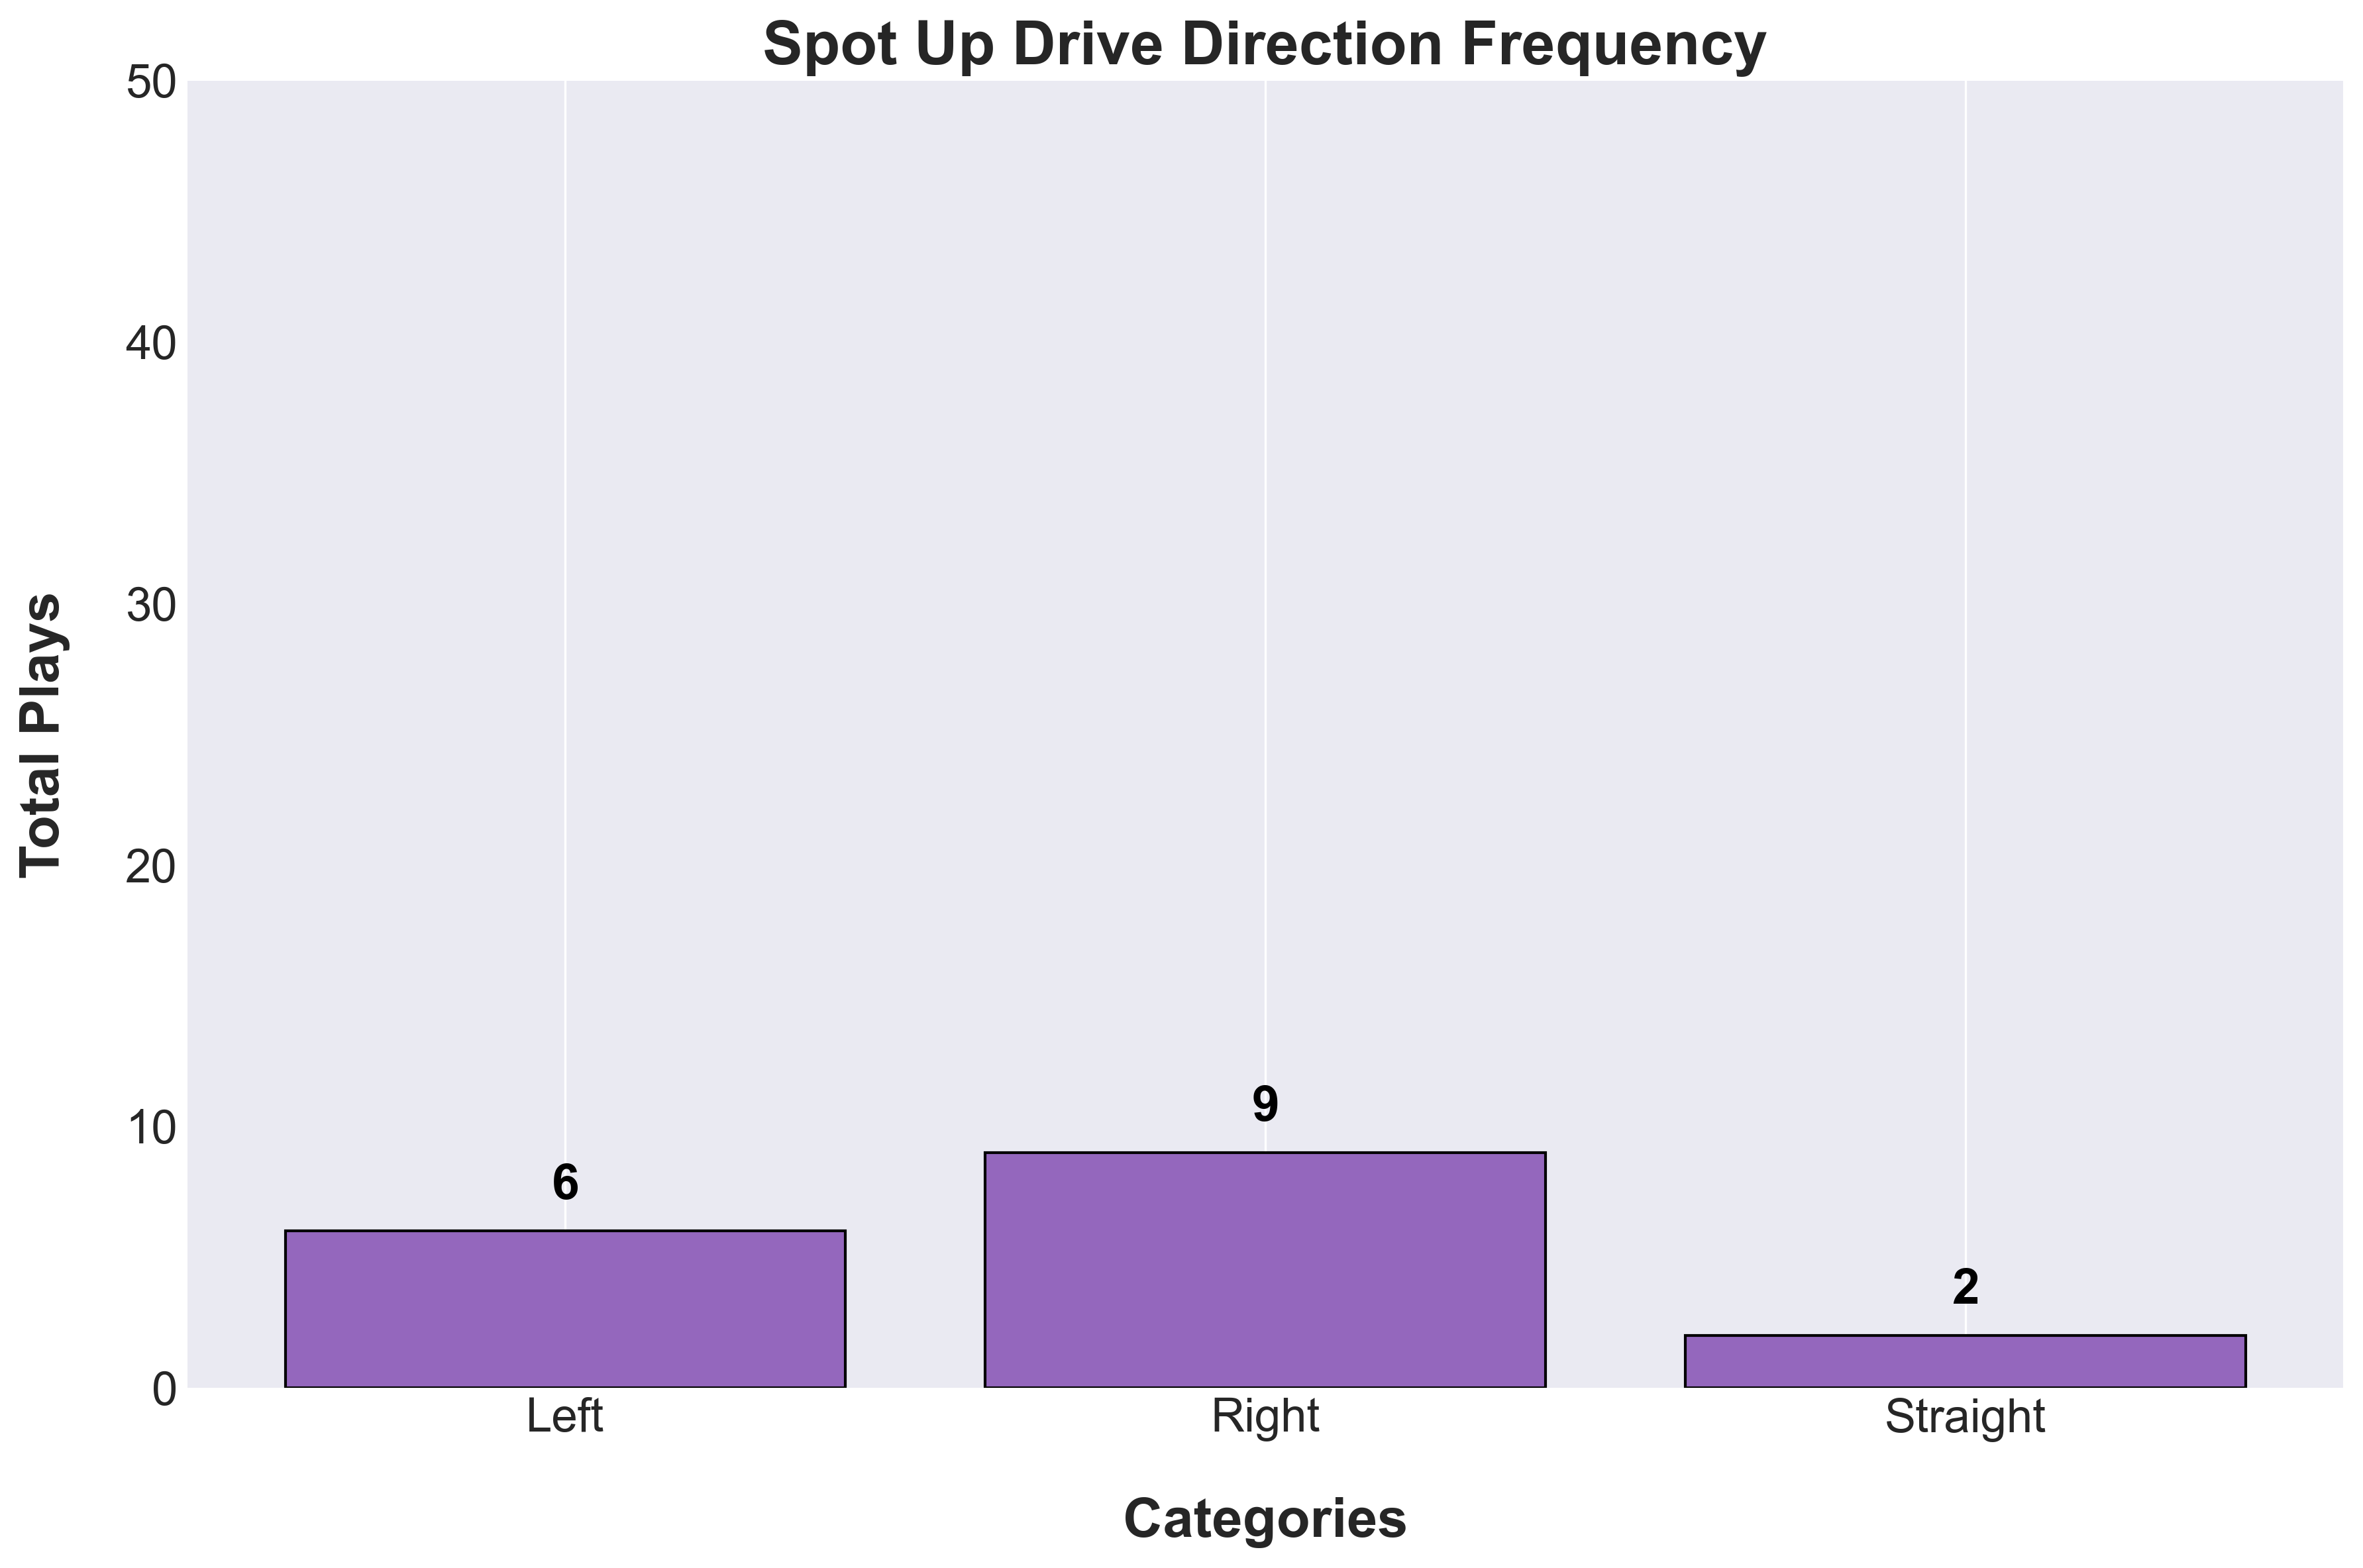
\includegraphics[width=\textwidth, height=.14\textheight]{images/SpotUp_DriveDirection_Freq.png} % Adjust the width of the image to fit
    \end{minipage}
    
\end{table}

\vspace{-1em} % Add vertical space before the line (optional)
\hrule height 1pt width 1\textwidth % Adjust height and width
\vspace{1 em} % Add vertical space after the line (optional)

\subsubsection{Stats on where Player gets Spot Ups from}

% Images of where they receive the ball SU Drives / Shots
\begin{table}[H]
    \centering
    \begin{minipage}[c]{0.45\textwidth} % First image minipage (45% of text width)
        \centering
        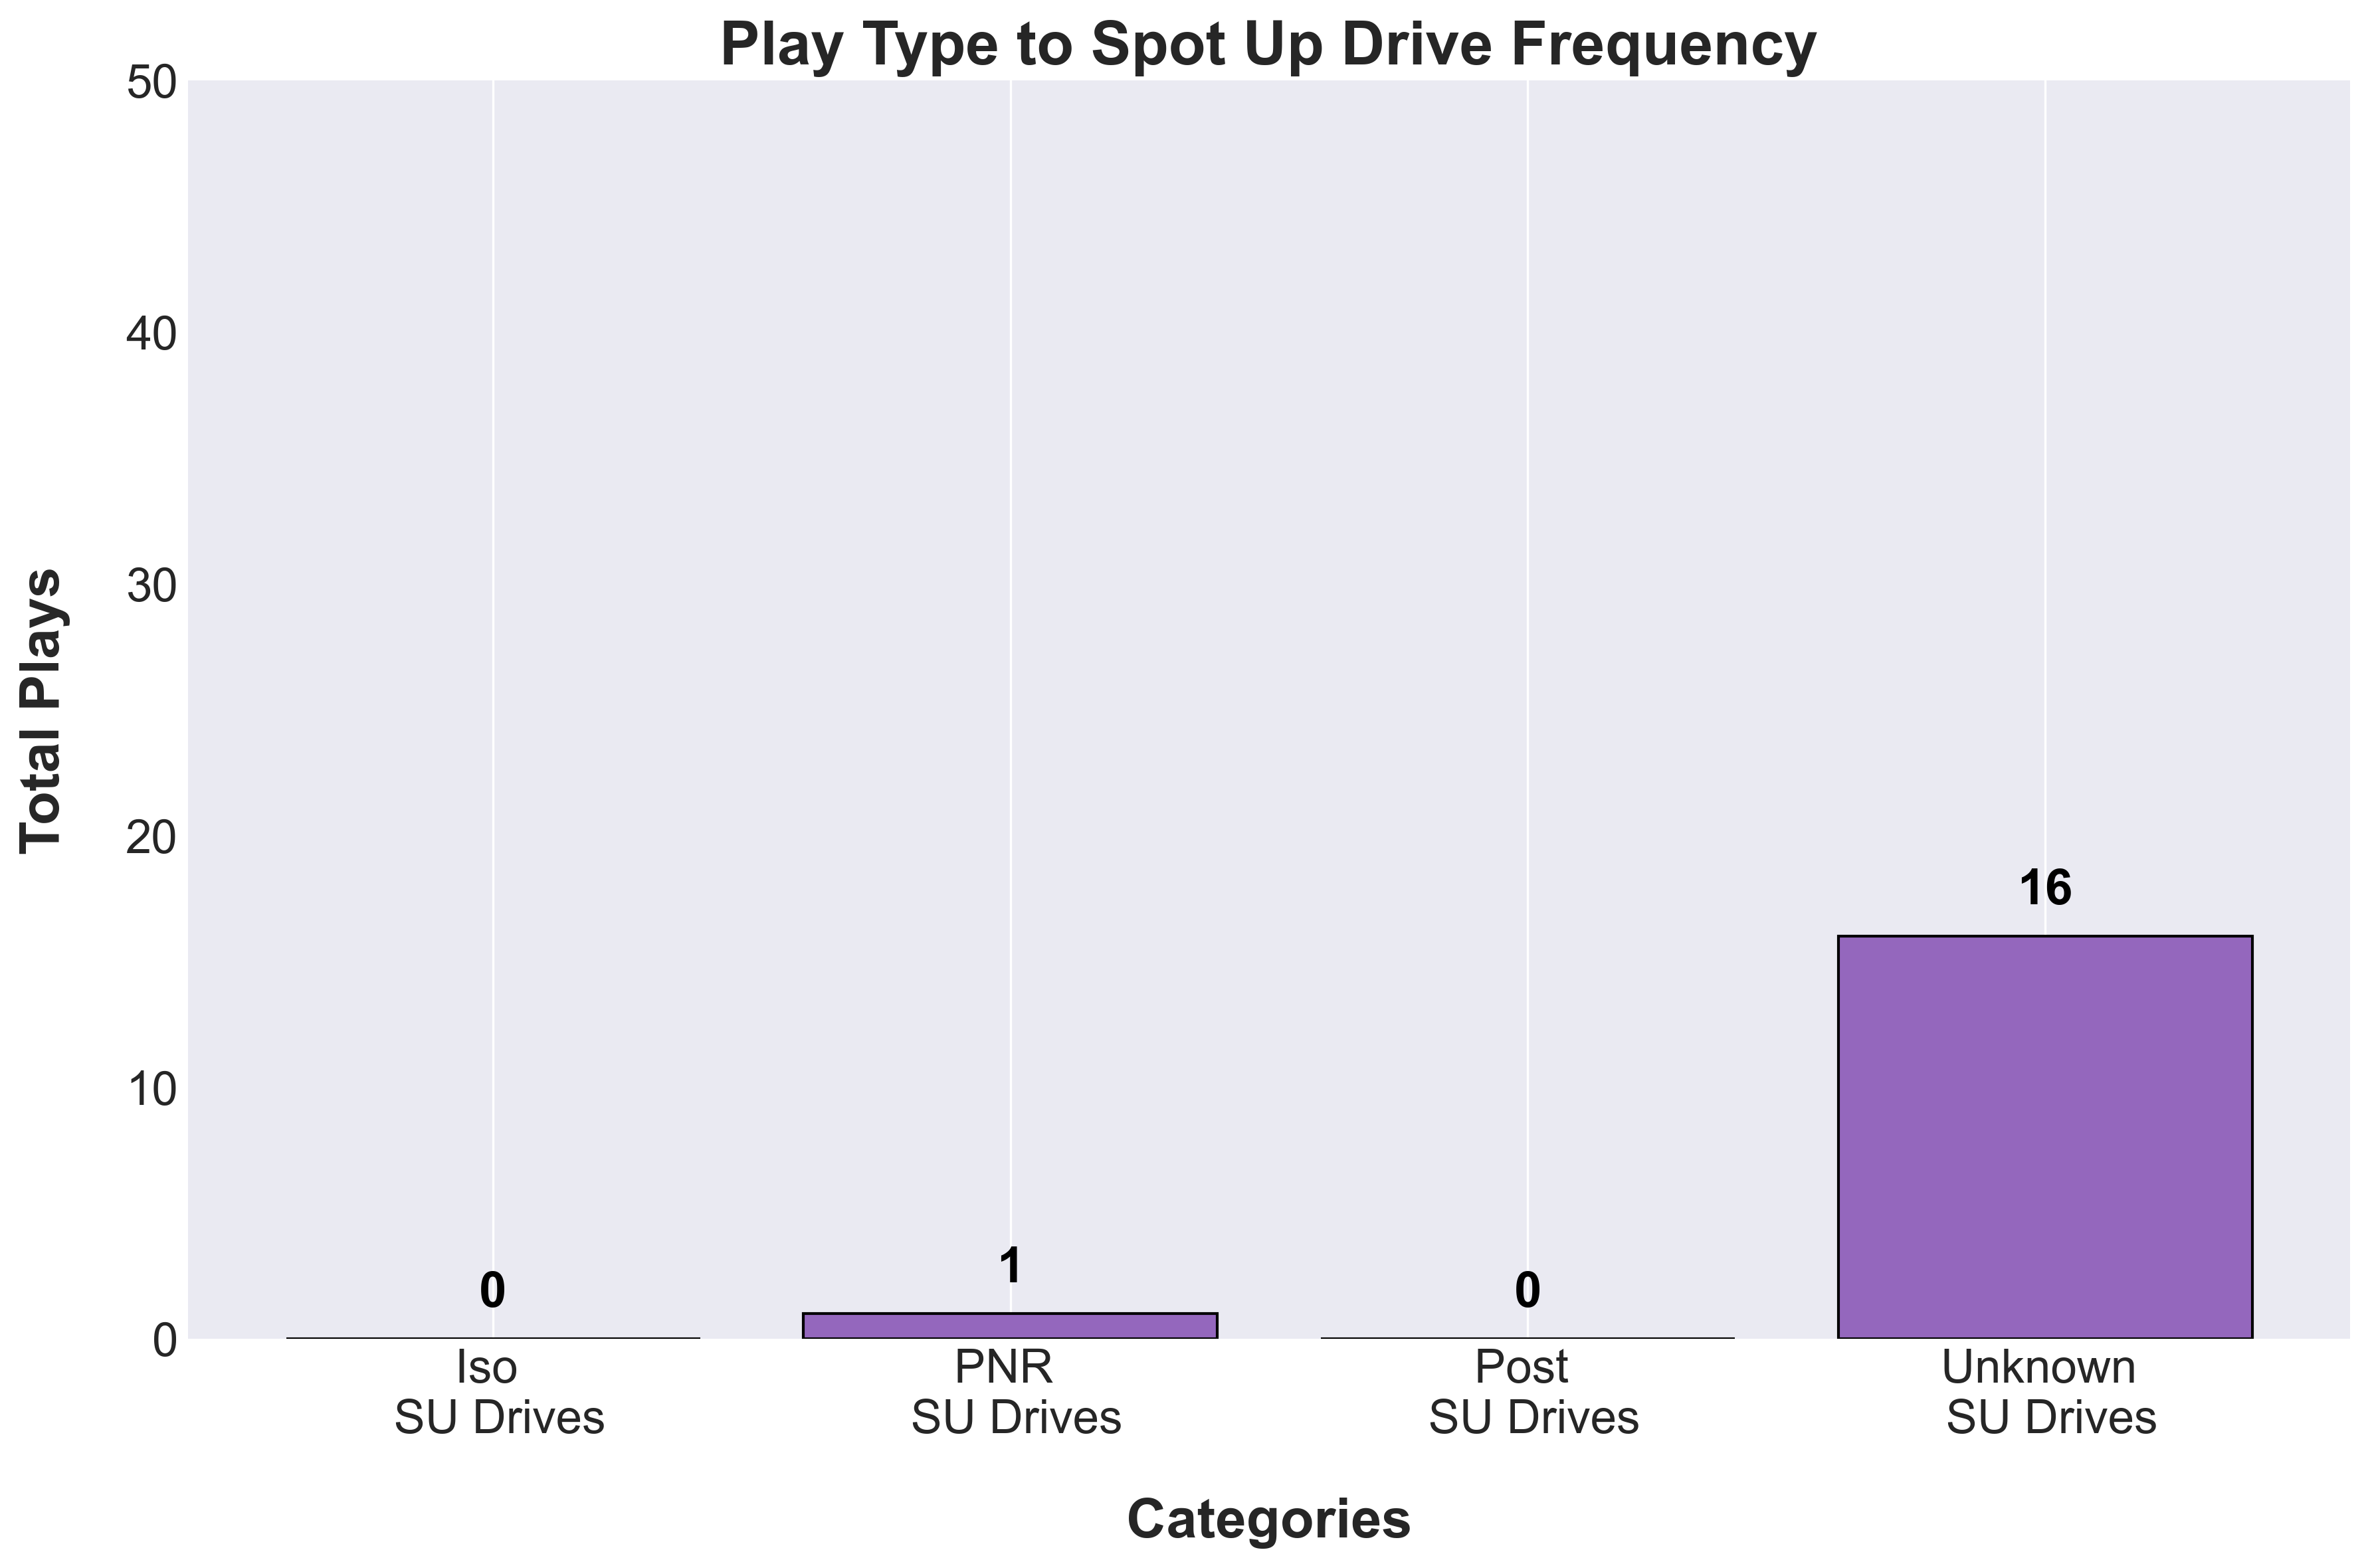
\includegraphics[width=.8\textwidth, height=0.15\textheight]{images/SpotUp_PlayTypeDrives_Freq.png} % Adjust image to fill the minipage but scale height to 3/4
    \end{minipage}
    \hfill % Flexible space between images
    \begin{minipage}[c]{0.45\textwidth} % Second image minipage (45% of text width)
        \centering
        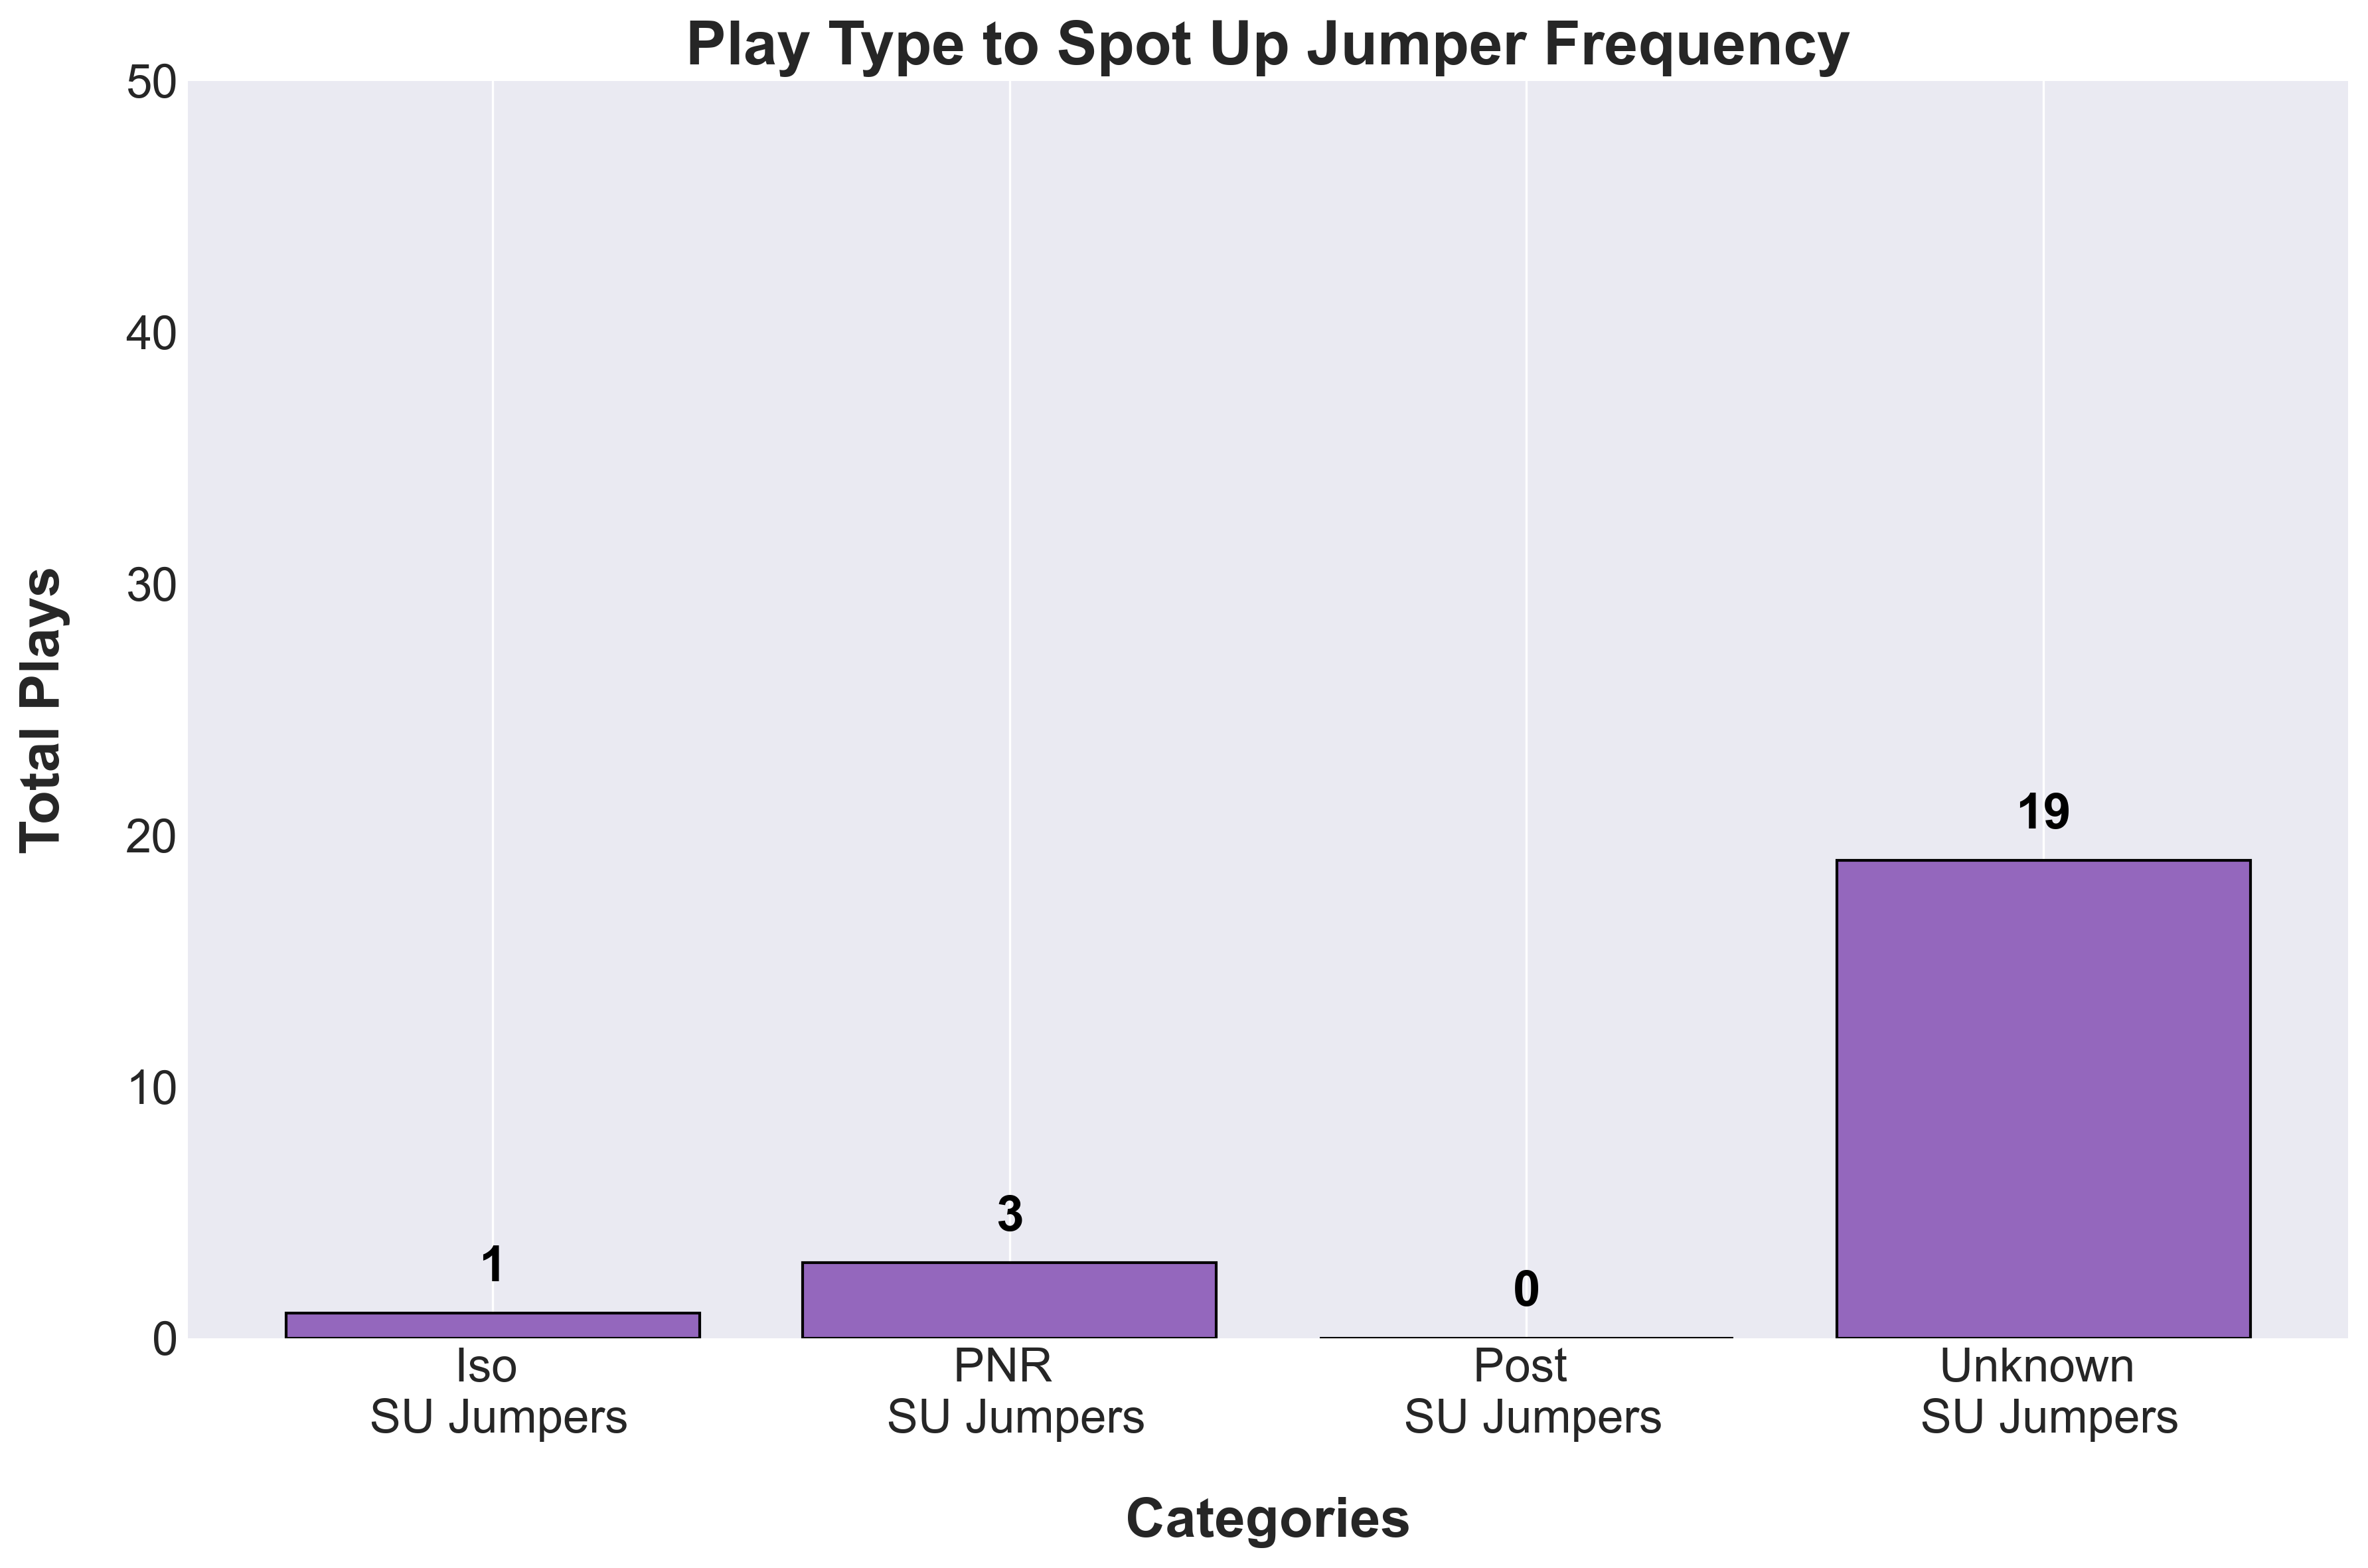
\includegraphics[width=.8\textwidth, height=0.15\textheight]{images/SpotUp_PlayTypeShots_Freq.png} % Adjust image to fill the minipage but scale height to 3/4
    \end{minipage}
\end{table}

\vspace{-1em} % Add vertical space before the line (optional)
\vspace{-1em} % Add vertical space after the line (optional)

% Tables of where they receive the ball SU Drives / Shots
\begin{table}[H]
    \centering
    \begin{minipage}[t]{0.45\textwidth} % Left table minipage
        \centering
        {\small \text{Different Playtype to Jumpshot Statistics}} % Center the title
        \vskip .25em % Adds vertical space between title and table
        \scalebox{.8}{ % Scale the entire table
            \scriptsize % Reduce the font size
            \renewcommand{\arraystretch}{1.3} % Adjust the number to increase or decrease row spacing
            \begin{tabular}{
            >{\centering\arraybackslash}p{1.25cm} 
            >{\centering\arraybackslash}p{.75cm} 
            >{\centering\arraybackslash}p{.5cm} 
            >{\centering\arraybackslash}p{.5cm}
            >{\centering\arraybackslash}p{.5cm} 
            >{\centering\arraybackslash}p{.5cm} 
            >{\centering\arraybackslash}p{.5cm}
            >{\centering\arraybackslash}p{.75cm}
            >{\centering\arraybackslash}p{.5cm} 
            >{\centering\arraybackslash}p{.5cm}}
            \toprule
            \textbf{PlayType} & \textbf{Plays} & \textbf{3PA} & \textbf{3PM} & \textbf{3P\%}  & \textbf{MiA} & \textbf{MiM} & \textbf{Mi\%}  & \textbf{TO} & \textbf{Foul} \\
            \midrule
            
                
            
                
            
                
            
                
            
                
            
                
                    Iso & 1 & 1 & 0 &
                    - & 
                    0 & 0 &
                    - &
                    0 & 0 \\
                
            
                
            
                
            
                
            
                
                    PNR & 4 & 4 & 2 &
                    - & 
                    0 & 0 &
                    - &
                    0 & 0 \\
                
            
                
            
                
            
                
            
                
            
                
            
                
            
                
            
                
            
                
            
                
            
                
            
                
            



            \bottomrule
        \end{tabular}
        }
    \end{minipage}
    \hfill % Flexible space between the two tables
    \begin{minipage}[t]{0.45\textwidth} % Right table minipage
        \centering
        {\small \text{Different Playtype to Drive Statistics}}% Center the title
        \vskip .25em % Adds vertical space between title and table
        \scalebox{.8}{ % Scale the entire table
            \scriptsize % Reduce the font size
            \renewcommand{\arraystretch}{1.3} % Adjust the number to increase or decrease row spacing
            \begin{tabular}{
            >{\centering\arraybackslash}p{1.25cm} 
            >{\centering\arraybackslash}p{.75cm} 
            >{\centering\arraybackslash}p{.5cm} 
            >{\centering\arraybackslash}p{.5cm}
            >{\centering\arraybackslash}p{.5cm} 
            >{\centering\arraybackslash}p{.5cm} 
            >{\centering\arraybackslash}p{.5cm}
            >{\centering\arraybackslash}p{.75cm}
            >{\centering\arraybackslash}p{.5cm} 
            >{\centering\arraybackslash}p{.5cm}}
            \toprule
            \textbf{PlayType} & \textbf{Plays} & \textbf{2PA} & \textbf{2PM} & \textbf{2P\%} & \textbf{MiA} & \textbf{MiM} & \textbf{Mi\%} & \textbf{TO} & \textbf{Foul} \\
            \midrule
            
                
            
                
            
                
            
                
            
                
            
                
            
                
            
                
                    PNR & 4 &
                    2 & 1 &
                    - &
                    0 & 0 &
                    - &
                    2 & 0 \\
                
            
                
            
                
            
                
            
                
                    Post & 2 &
                    2 & 2 &
                    - &
                    1 & 1 &
                    - &
                    0 & 0 \\
                
            
                
            
                
            
                
            
                
            
                
            
                
            
                
            
                
            
                
            
                
            

            
            \bottomrule
        \end{tabular}
        }
    \end{minipage}
\end{table}

\vspace{1em} % Add vertical space before the line (optional)
\vspace{-1em} % Add vertical space after the line (optional)

% Post -> Jumpshot Stats by Passer
\begin{table}[H]
    \raisebox{3em}{ % Adjust this value to shift the tables vertically
    \begin{minipage}[t]{0.6\textwidth} % Left side (table) takes 85% of the width
        \flushleft
        \centering % Centering the title and the table
        \text{Post - Jumpshot Stats by Passer} % Title above the table in bold
        \vskip .25em % Adds vertical space between title and table
        \scalebox{.6}{ % Scale the entire table down by half
            \renewcommand{\arraystretch}{1.4} % Adjust the number to increase or decrease row spacing
            \begin{tabular}{
            >{\centering\arraybackslash}p{1.75cm} 
            >{\centering\arraybackslash}p{.75cm} 
            >{\centering\arraybackslash}p{.75cm} 
            >{\centering\arraybackslash}p{.75cm} 
            >{\centering\arraybackslash}p{.75cm}
            >{\centering\arraybackslash}p{.75cm} 
            >{\centering\arraybackslash}p{.75cm} 
            >{\centering\arraybackslash}p{.75cm} 
            >{\centering\arraybackslash}p{.75cm}
            >{\centering\arraybackslash}p{.75cm} 
            >{\centering\arraybackslash}p{.75cm}
            >{\centering\arraybackslash}p{.75cm}
            >{\centering\arraybackslash}p{.75cm} 
            >{\centering\arraybackslash}p{.75cm}}% Adjust column widths
            \toprule
            {\scriptsize \textbf{Player}} &
            {\scriptsize \textbf{Plays}} &
            {\scriptsize \textbf{3PA}} &
            {\scriptsize \textbf{3PM}} &
            {\scriptsize \textbf{3P\%}} & 
            {\scriptsize \textbf{2PA}} & 
            {\scriptsize \textbf{2PM}} & 
            {\scriptsize \textbf{2P\%}} & 
            {\scriptsize \textbf{MiA}} & 
            {\scriptsize \textbf{MiM}} &
            {\scriptsize \textbf{Mi\%}} &
            {\scriptsize \textbf{EFG\%}} &
            {\scriptsize \textbf{TO}} &
            {\scriptsize \textbf{Foul}} \\
            \midrule
            
                
            
                
            
                
            
                
            
                
            
                
            
                
            
                
            
                
            
                
            
                
            
                
            
                
            
                
            
                
                    
                
            
                
            
                
            
                
            
                
            
                
            
                
            
                
            

            \bottomrule
        \end{tabular}
        } % End of \scalebox
    \end{minipage}
    } % End of raisebox, closing the adjustment
    \hfill % This adds some flexible space between the table and the image
    \begin{minipage}[c]{0.35\textwidth} % Right side (image) takes 10% of the width
        \flushright
        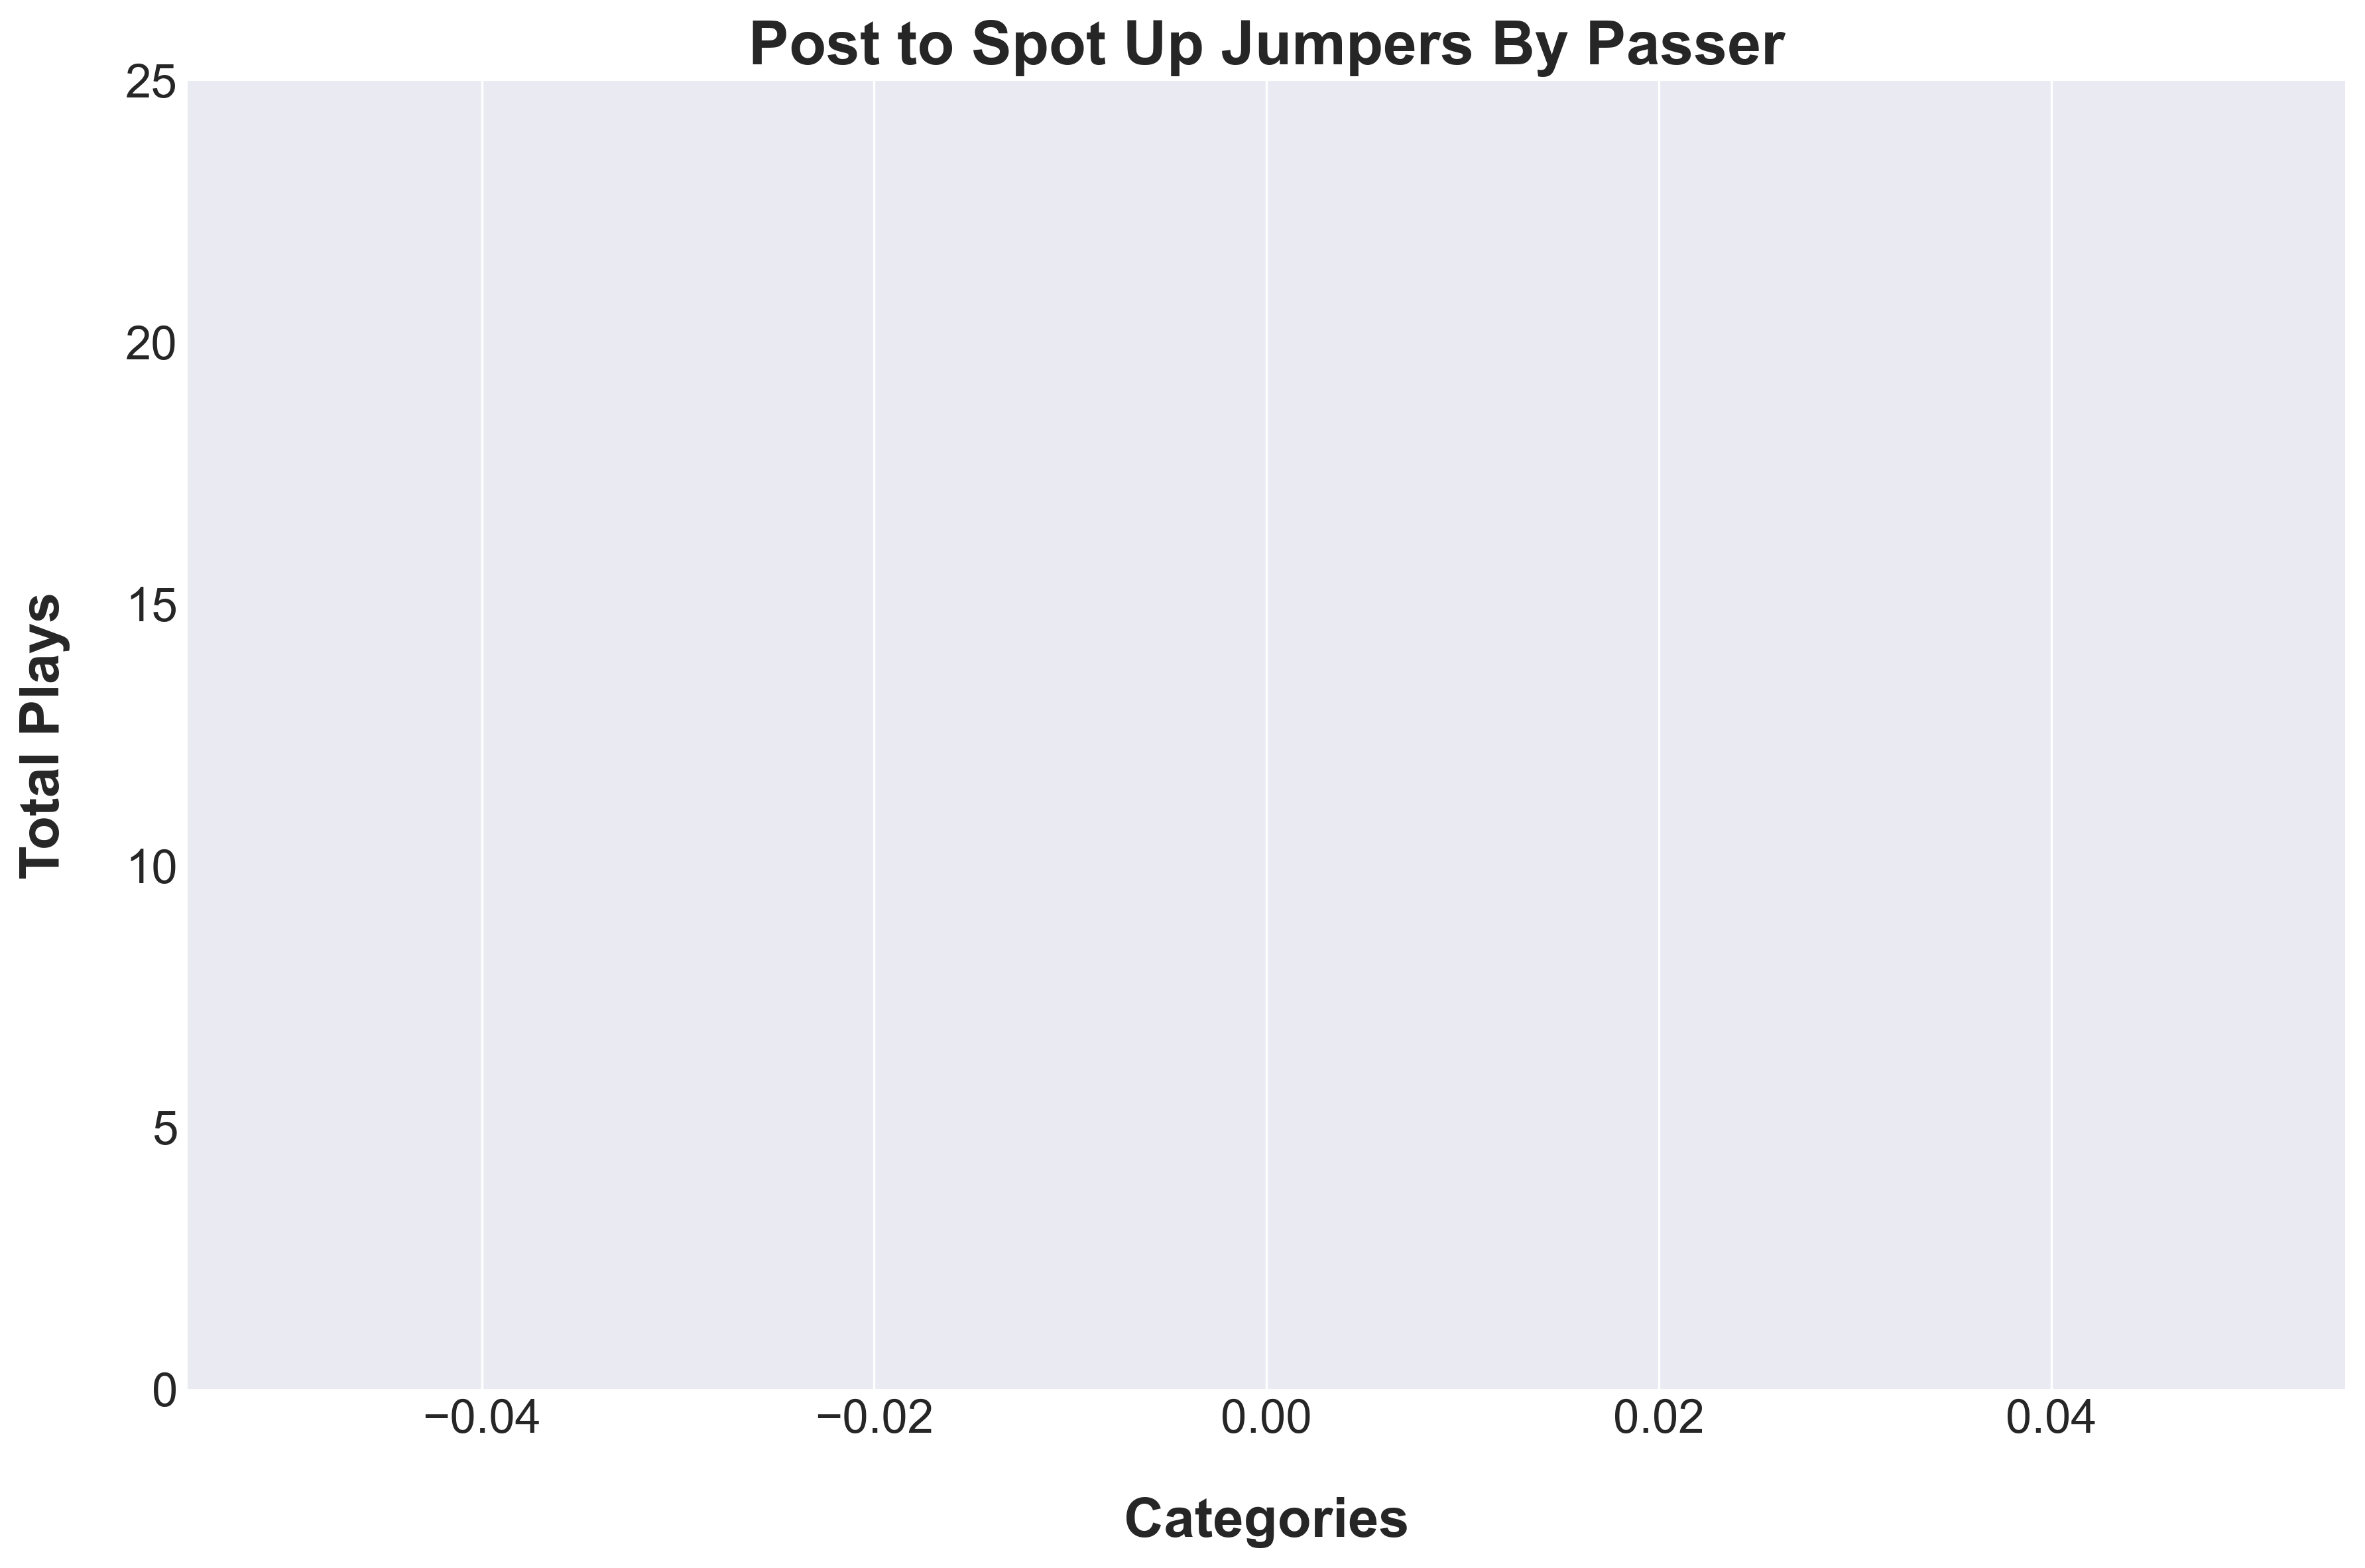
\includegraphics[width=\textwidth, height=.14\textheight]{images/SpotUp_PostShotsPlayer_Freq.png} % Adjust the width of the image to fit
    \end{minipage}
\end{table}

\vspace{-1em} % Add vertical space before the line (optional)
\vspace{-1em} % Add vertical space after the line (optional)

% Iso -> Jumpshot Stats by Passer
\begin{table}[H]
    \raisebox{3em}{ % Adjust this value to shift the tables vertically
    \begin{minipage}[t]{0.6\textwidth} % Left side (table) takes 85% of the width
        \flushleft
        \centering % Centering the title and the table
        \text{Iso - Jumpshot Stats by Passer} % Title above the table in bold
        \vskip .25em % Adds vertical space between title and table
        \scalebox{.6}{ % Scale the entire table down by half
            \renewcommand{\arraystretch}{1.4} % Adjust the number to increase or decrease row spacing
            \begin{tabular}{
            >{\centering\arraybackslash}p{1.75cm} 
            >{\centering\arraybackslash}p{.75cm} 
            >{\centering\arraybackslash}p{.75cm} 
            >{\centering\arraybackslash}p{.75cm} 
            >{\centering\arraybackslash}p{.75cm}
            >{\centering\arraybackslash}p{.75cm} 
            >{\centering\arraybackslash}p{.75cm} 
            >{\centering\arraybackslash}p{.75cm} 
            >{\centering\arraybackslash}p{.75cm}
            >{\centering\arraybackslash}p{.75cm} 
            >{\centering\arraybackslash}p{.75cm}
            >{\centering\arraybackslash}p{.75cm}
            >{\centering\arraybackslash}p{.75cm} 
            >{\centering\arraybackslash}p{.75cm}}% Adjust column widths
            \toprule
            {\scriptsize \textbf{Player}} &
            {\scriptsize \textbf{Plays}} &
            {\scriptsize \textbf{3PA}} &
            {\scriptsize \textbf{3PM}} &
            {\scriptsize \textbf{3P\%}} & 
            {\scriptsize \textbf{2PA}} & 
            {\scriptsize \textbf{2PM}} & 
            {\scriptsize \textbf{2P\%}} & 
            {\scriptsize \textbf{MiA}} & 
            {\scriptsize \textbf{MiM}} &
            {\scriptsize \textbf{Mi\%}} &
            {\scriptsize \textbf{EFG\%}} &
            {\scriptsize \textbf{TO}} &
            {\scriptsize \textbf{Foul}} \\
            \midrule
            
                
            
                
            
                
            
                
            
                
            
                
            
                
                    
                        Brock Bowen & 
                        1 & 
                        1 & 
                        0 & 
                        - & 
                        0 & 
                        0 & 
                        - & 
                        0 & 
                        0 & 
                        - & 
                        - & 
                        0 & 
                        0 \\
                    
                
            
                
            
                
            
                
            
                
            
                
            
                
            
                
            
                
            
                
            
                
            
                
            
                
            
                
            
                
            
                
            
            \bottomrule
        \end{tabular}
        } % End of \scalebox
    \end{minipage}
    } % End of raisebox, closing the adjustment
    \hfill % This adds some flexible space between the table and the image
    \begin{minipage}[c]{0.35\textwidth} % Right side (image) takes 10% of the width
        \flushright
        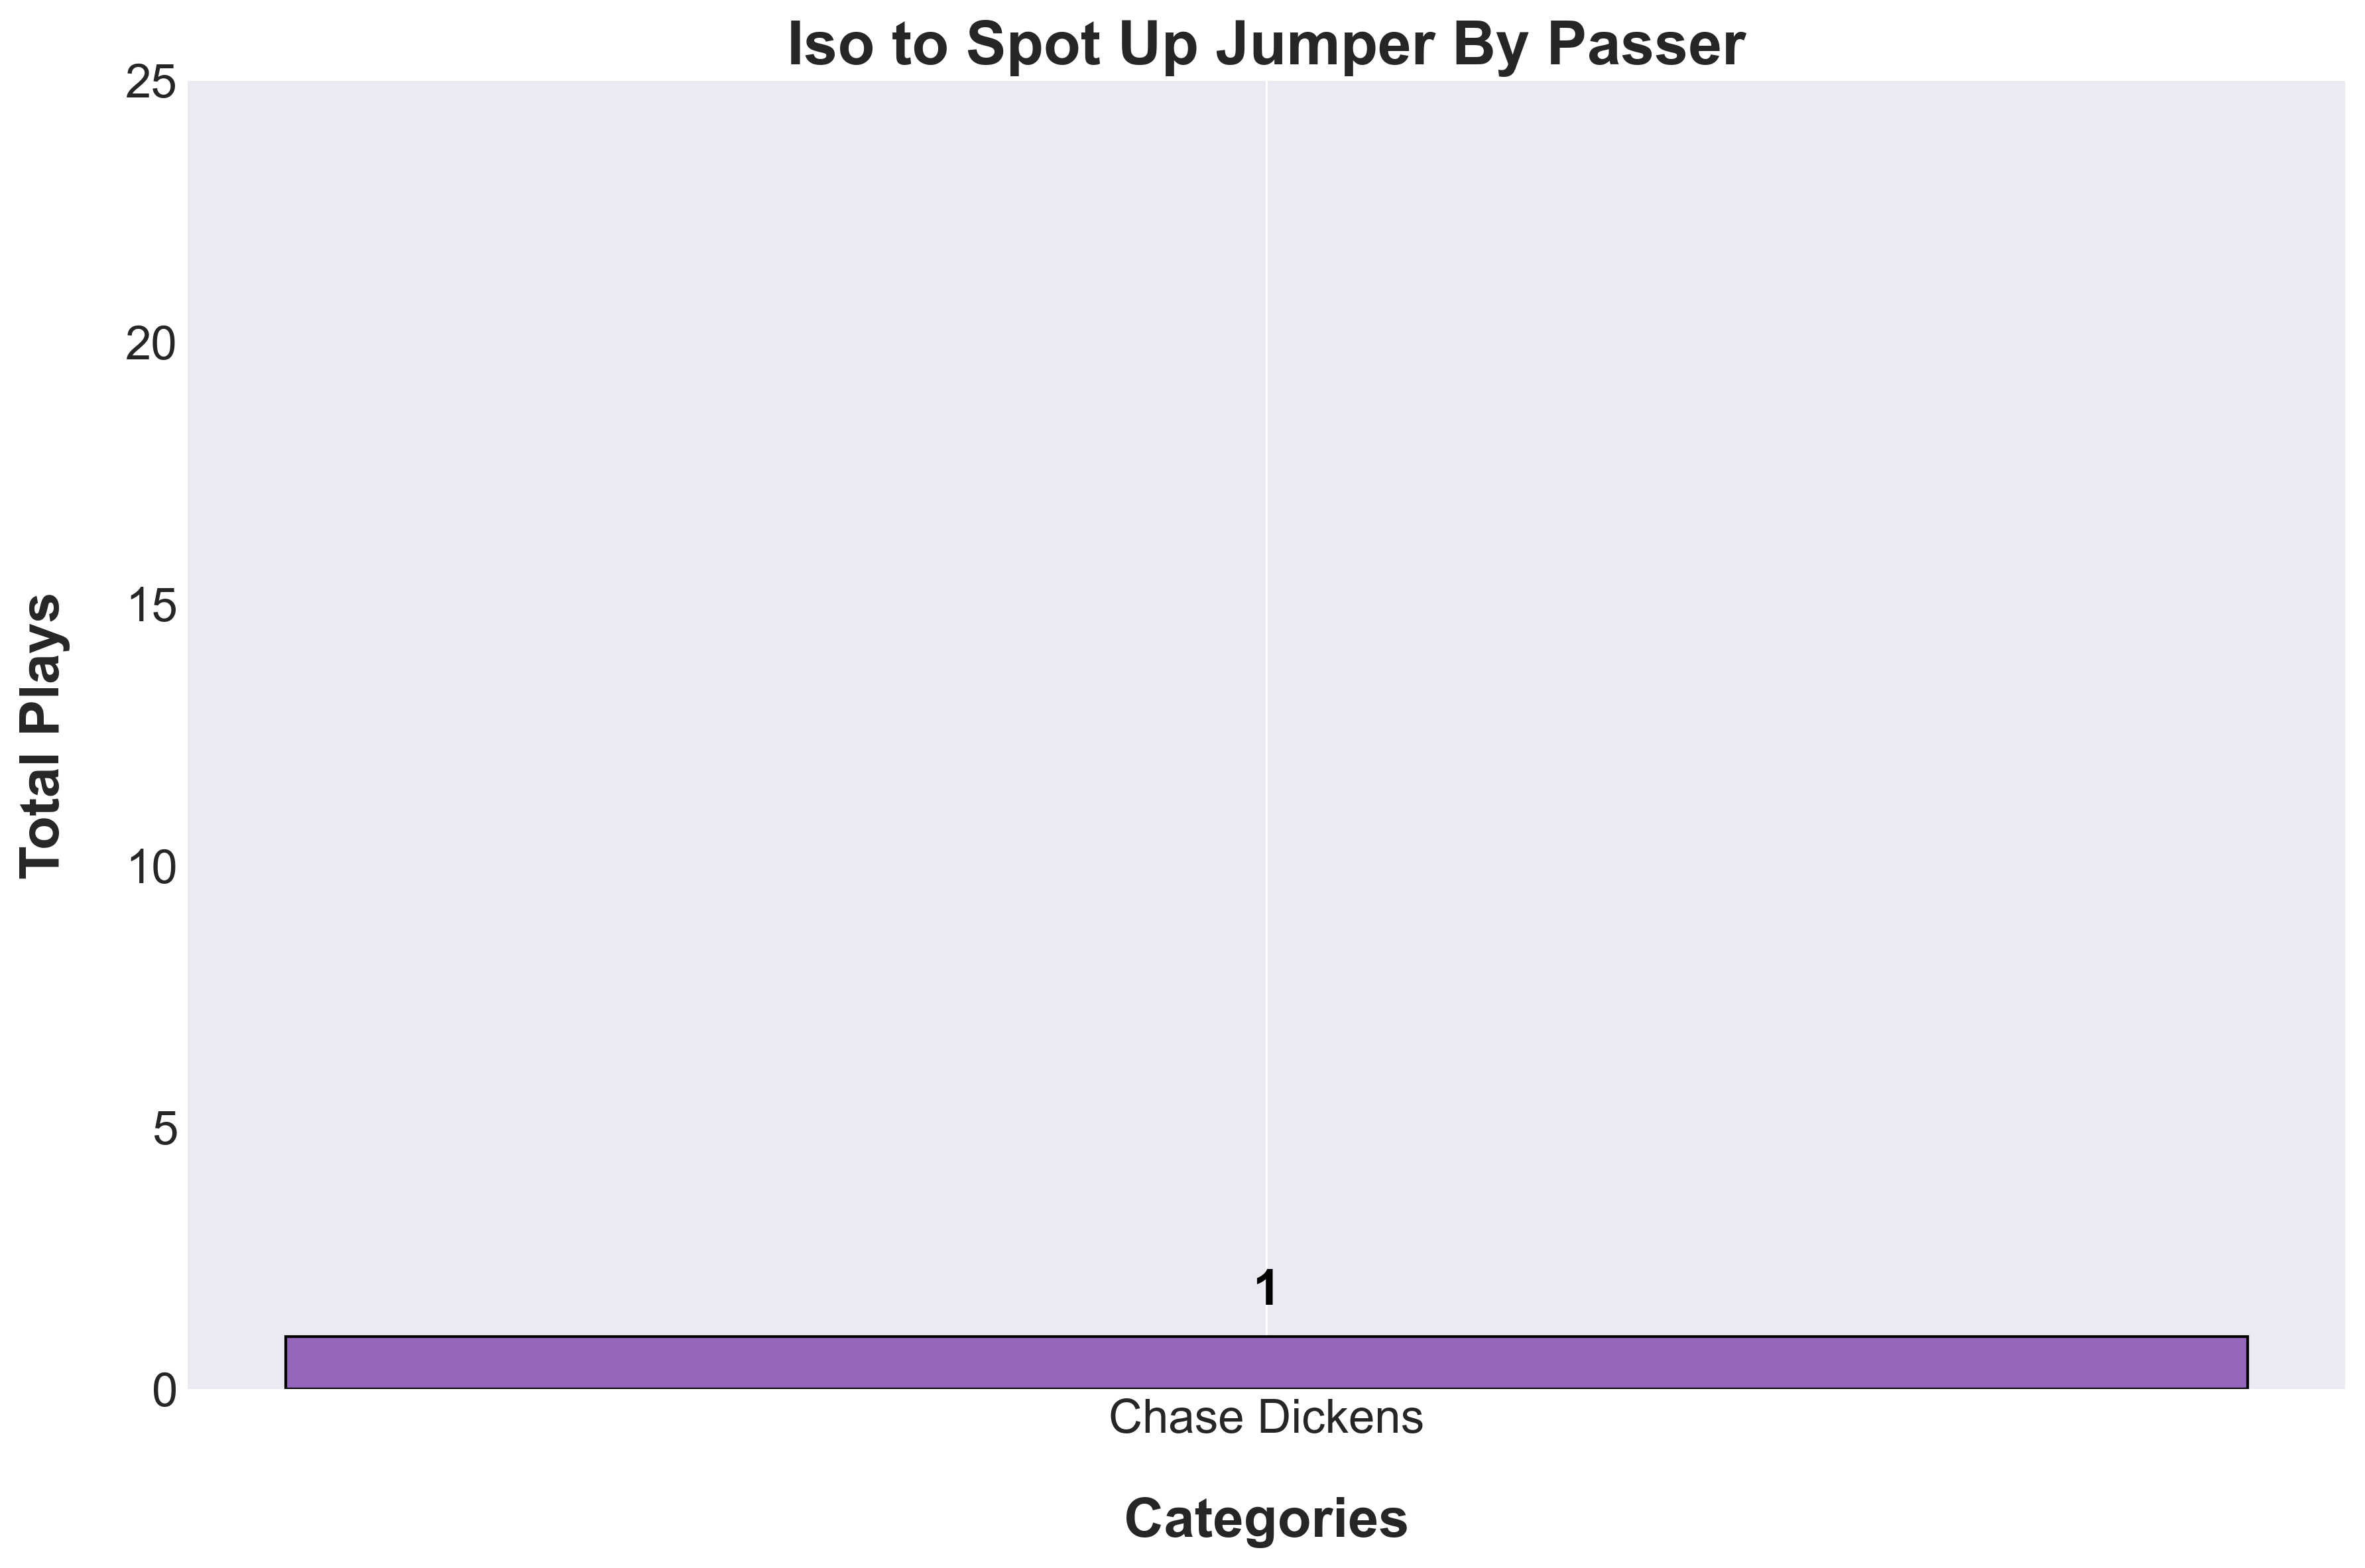
\includegraphics[width=\textwidth, height=.14\textheight]{images/SpotUp_IsoShotsPlayer_Freq.png} % Adjust the width of the image to fit
    \end{minipage}
\end{table}

\vspace{-1em} % Add vertical space before the line (optional)
\vspace{-1em} % Add vertical space after the line (optional)

% PNR -> Jumpshot Stats by Passer
\begin{table}[H]
    \raisebox{3em}{ % Adjust this value to shift the tables vertically
    \begin{minipage}[t]{0.6\textwidth} % Left side (table) takes 85% of the width
        \flushleft
        \centering % Centering the title and the table
        \text{PNR - Jumpshot Stats by Passer} % Title above the table in bold
        \vskip .25em % Adds vertical space between title and table
        \scalebox{.6}{ % Scale the entire table down by half
            \renewcommand{\arraystretch}{1.4} % Adjust the number to increase or decrease row spacing
            \begin{tabular}{
            >{\centering\arraybackslash}p{1.75cm} 
            >{\centering\arraybackslash}p{.75cm} 
            >{\centering\arraybackslash}p{.75cm} 
            >{\centering\arraybackslash}p{.75cm} 
            >{\centering\arraybackslash}p{.75cm}
            >{\centering\arraybackslash}p{.75cm} 
            >{\centering\arraybackslash}p{.75cm} 
            >{\centering\arraybackslash}p{.75cm} 
            >{\centering\arraybackslash}p{.75cm}
            >{\centering\arraybackslash}p{.75cm} 
            >{\centering\arraybackslash}p{.75cm}
            >{\centering\arraybackslash}p{.75cm}
            >{\centering\arraybackslash}p{.75cm} 
            >{\centering\arraybackslash}p{.75cm}}% Adjust column widths
            \toprule
            {\scriptsize \textbf{Player}} &
            {\scriptsize \textbf{Plays}} &
            {\scriptsize \textbf{3PA}} &
            {\scriptsize \textbf{3PM}} &
            {\scriptsize \textbf{3P\%}} & 
            {\scriptsize \textbf{2PA}} & 
            {\scriptsize \textbf{2PM}} & 
            {\scriptsize \textbf{2P\%}} & 
            {\scriptsize \textbf{MiA}} & 
            {\scriptsize \textbf{MiM}} &
            {\scriptsize \textbf{Mi\%}} &
            {\scriptsize \textbf{EFG\%}} &
            {\scriptsize \textbf{TO}} &
            {\scriptsize \textbf{Foul}} \\
            \midrule
            
                
            
                
            
                
            
                
            
                
            
                
            
                
            
                
            
                
            
                
            
                
                    
                        Brock Bowen & 
                        3 & 
                        3 & 
                        2 & 
                        - & 
                        0 & 
                        0 & 
                        - & 
                        0 & 
                        0 & 
                        - & 
                        - & 
                        0 & 
                        0 \\
                    
                        Chase Dickens & 
                        1 & 
                        1 & 
                        0 & 
                        - & 
                        0 & 
                        0 & 
                        - & 
                        0 & 
                        0 & 
                        - & 
                        - & 
                        0 & 
                        0 \\
                    
                
            
                
            
                
            
                
            
                
            
                
            
                
            
                
            
                
            
                
            
                
            
                
            

            \bottomrule
        \end{tabular}
        } % End of \scalebox
    \end{minipage}
    } % End of raisebox, closing the adjustment
    \hfill % This adds some flexible space between the table and the image
    \begin{minipage}[c]{0.35\textwidth} % Right side (image) takes 10% of the width
        \flushright
        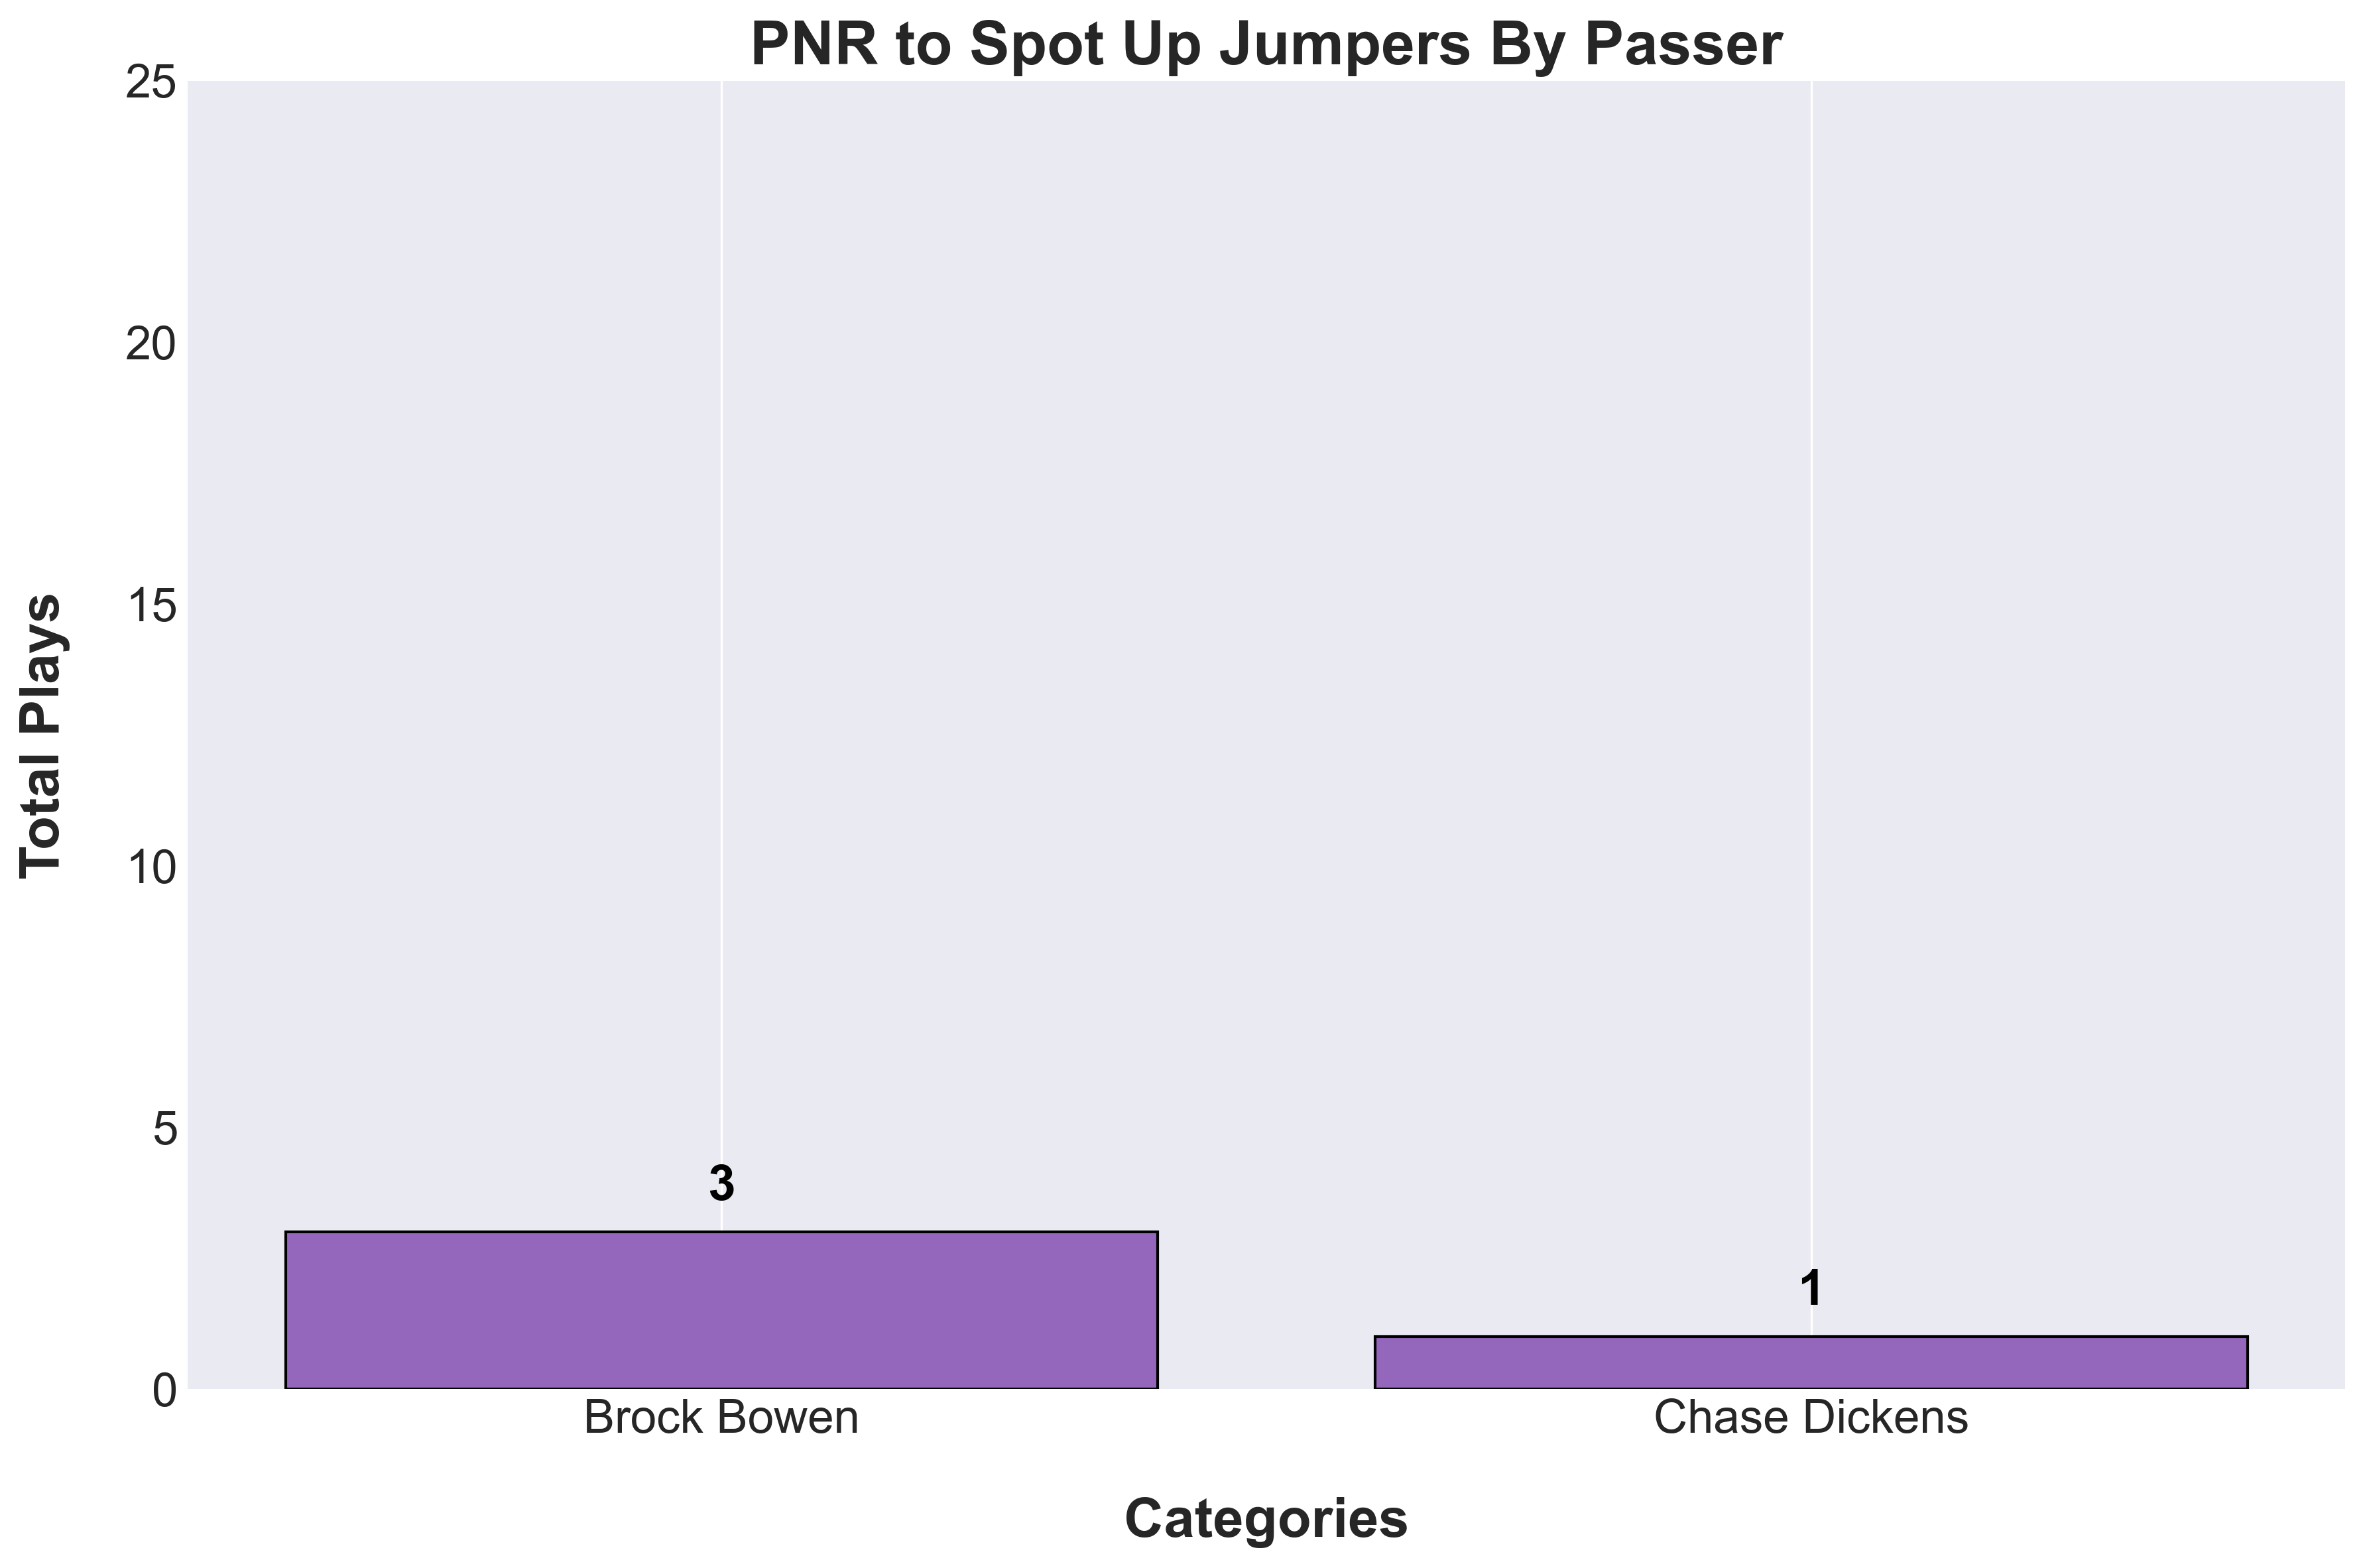
\includegraphics[width=\textwidth, height=.14\textheight]{images/SpotUp_PNRShotsPlayer_Freq.png} % Adjust the width of the image to fit
    \end{minipage}
\end{table}

\vspace{-1em} % Add vertical space before the line (optional)
\vspace{-1em} % Add vertical space after the line (optional)

% Post -> Drive Stats by Passer
\begin{table}[H]
    \raisebox{3em}{ % Adjust this value to shift the tables vertically
    \begin{minipage}[t]{0.6\textwidth} % Left side (table) takes 85% of the width
        \flushleft
        \centering % Centering the title and the table
        \text{Post - Drive Stats by Passer} % Title above the table in bold
        \vskip .25em % Adds vertical space between title and table
        \scalebox{.6}{ % Scale the entire table down by half
            \renewcommand{\arraystretch}{1.4} % Adjust the number to increase or decrease row spacing
            \begin{tabular}{
            >{\centering\arraybackslash}p{1.75cm} 
            >{\centering\arraybackslash}p{.75cm} 
            >{\centering\arraybackslash}p{.75cm} 
            >{\centering\arraybackslash}p{.75cm} 
            >{\centering\arraybackslash}p{.75cm}
            >{\centering\arraybackslash}p{.75cm} 
            >{\centering\arraybackslash}p{.75cm} 
            >{\centering\arraybackslash}p{.75cm} 
            >{\centering\arraybackslash}p{.75cm}
            >{\centering\arraybackslash}p{.75cm} 
            >{\centering\arraybackslash}p{.75cm}
            >{\centering\arraybackslash}p{.75cm}
            >{\centering\arraybackslash}p{.75cm} 
            >{\centering\arraybackslash}p{.75cm}}% Adjust column widths
            \toprule
            {\scriptsize \textbf{Player}} &
            {\scriptsize \textbf{Plays}} &
            {\scriptsize \textbf{3PA}} &
            {\scriptsize \textbf{3PM}} &
            {\scriptsize \textbf{3P\%}} & 
            {\scriptsize \textbf{2PA}} & 
            {\scriptsize \textbf{2PM}} & 
            {\scriptsize \textbf{2P\%}} & 
            {\scriptsize \textbf{MiA}} & 
            {\scriptsize \textbf{MiM}} &
            {\scriptsize \textbf{Mi\%}} &
            {\scriptsize \textbf{EFG\%}} &
            {\scriptsize \textbf{TO}} &
            {\scriptsize \textbf{Foul}} \\
            \midrule
            
                
            
                
            
                
            
                
            
                
            
                
            
                
            
                
            
                
            
                
            
                
            
                
            
                
                    
                        Josiah Turner & 
                        1 & 
                        0 & 
                        0 & 
                        - & 
                        1 & 
                        1 & 
                        - & 
                        1 & 
                        1 & 
                        - & 
                        - & 
                        0 & 
                        0 \\
                    
                        Kenny Wilburn & 
                        1 & 
                        0 & 
                        0 & 
                        - & 
                        1 & 
                        1 & 
                        - & 
                        0 & 
                        0 & 
                        - & 
                        - & 
                        0 & 
                        0 \\
                    
                
            
                
            
                
            
                
            
                
            
                
            
                
            
                
            
                
            
                
            

            \bottomrule
        \end{tabular}
        } % End of \scalebox
    \end{minipage}
    } % End of raisebox, closing the adjustment
    \hfill % This adds some flexible space between the table and the image
    \begin{minipage}[c]{0.35\textwidth} % Right side (image) takes 10% of the width
        \flushright
        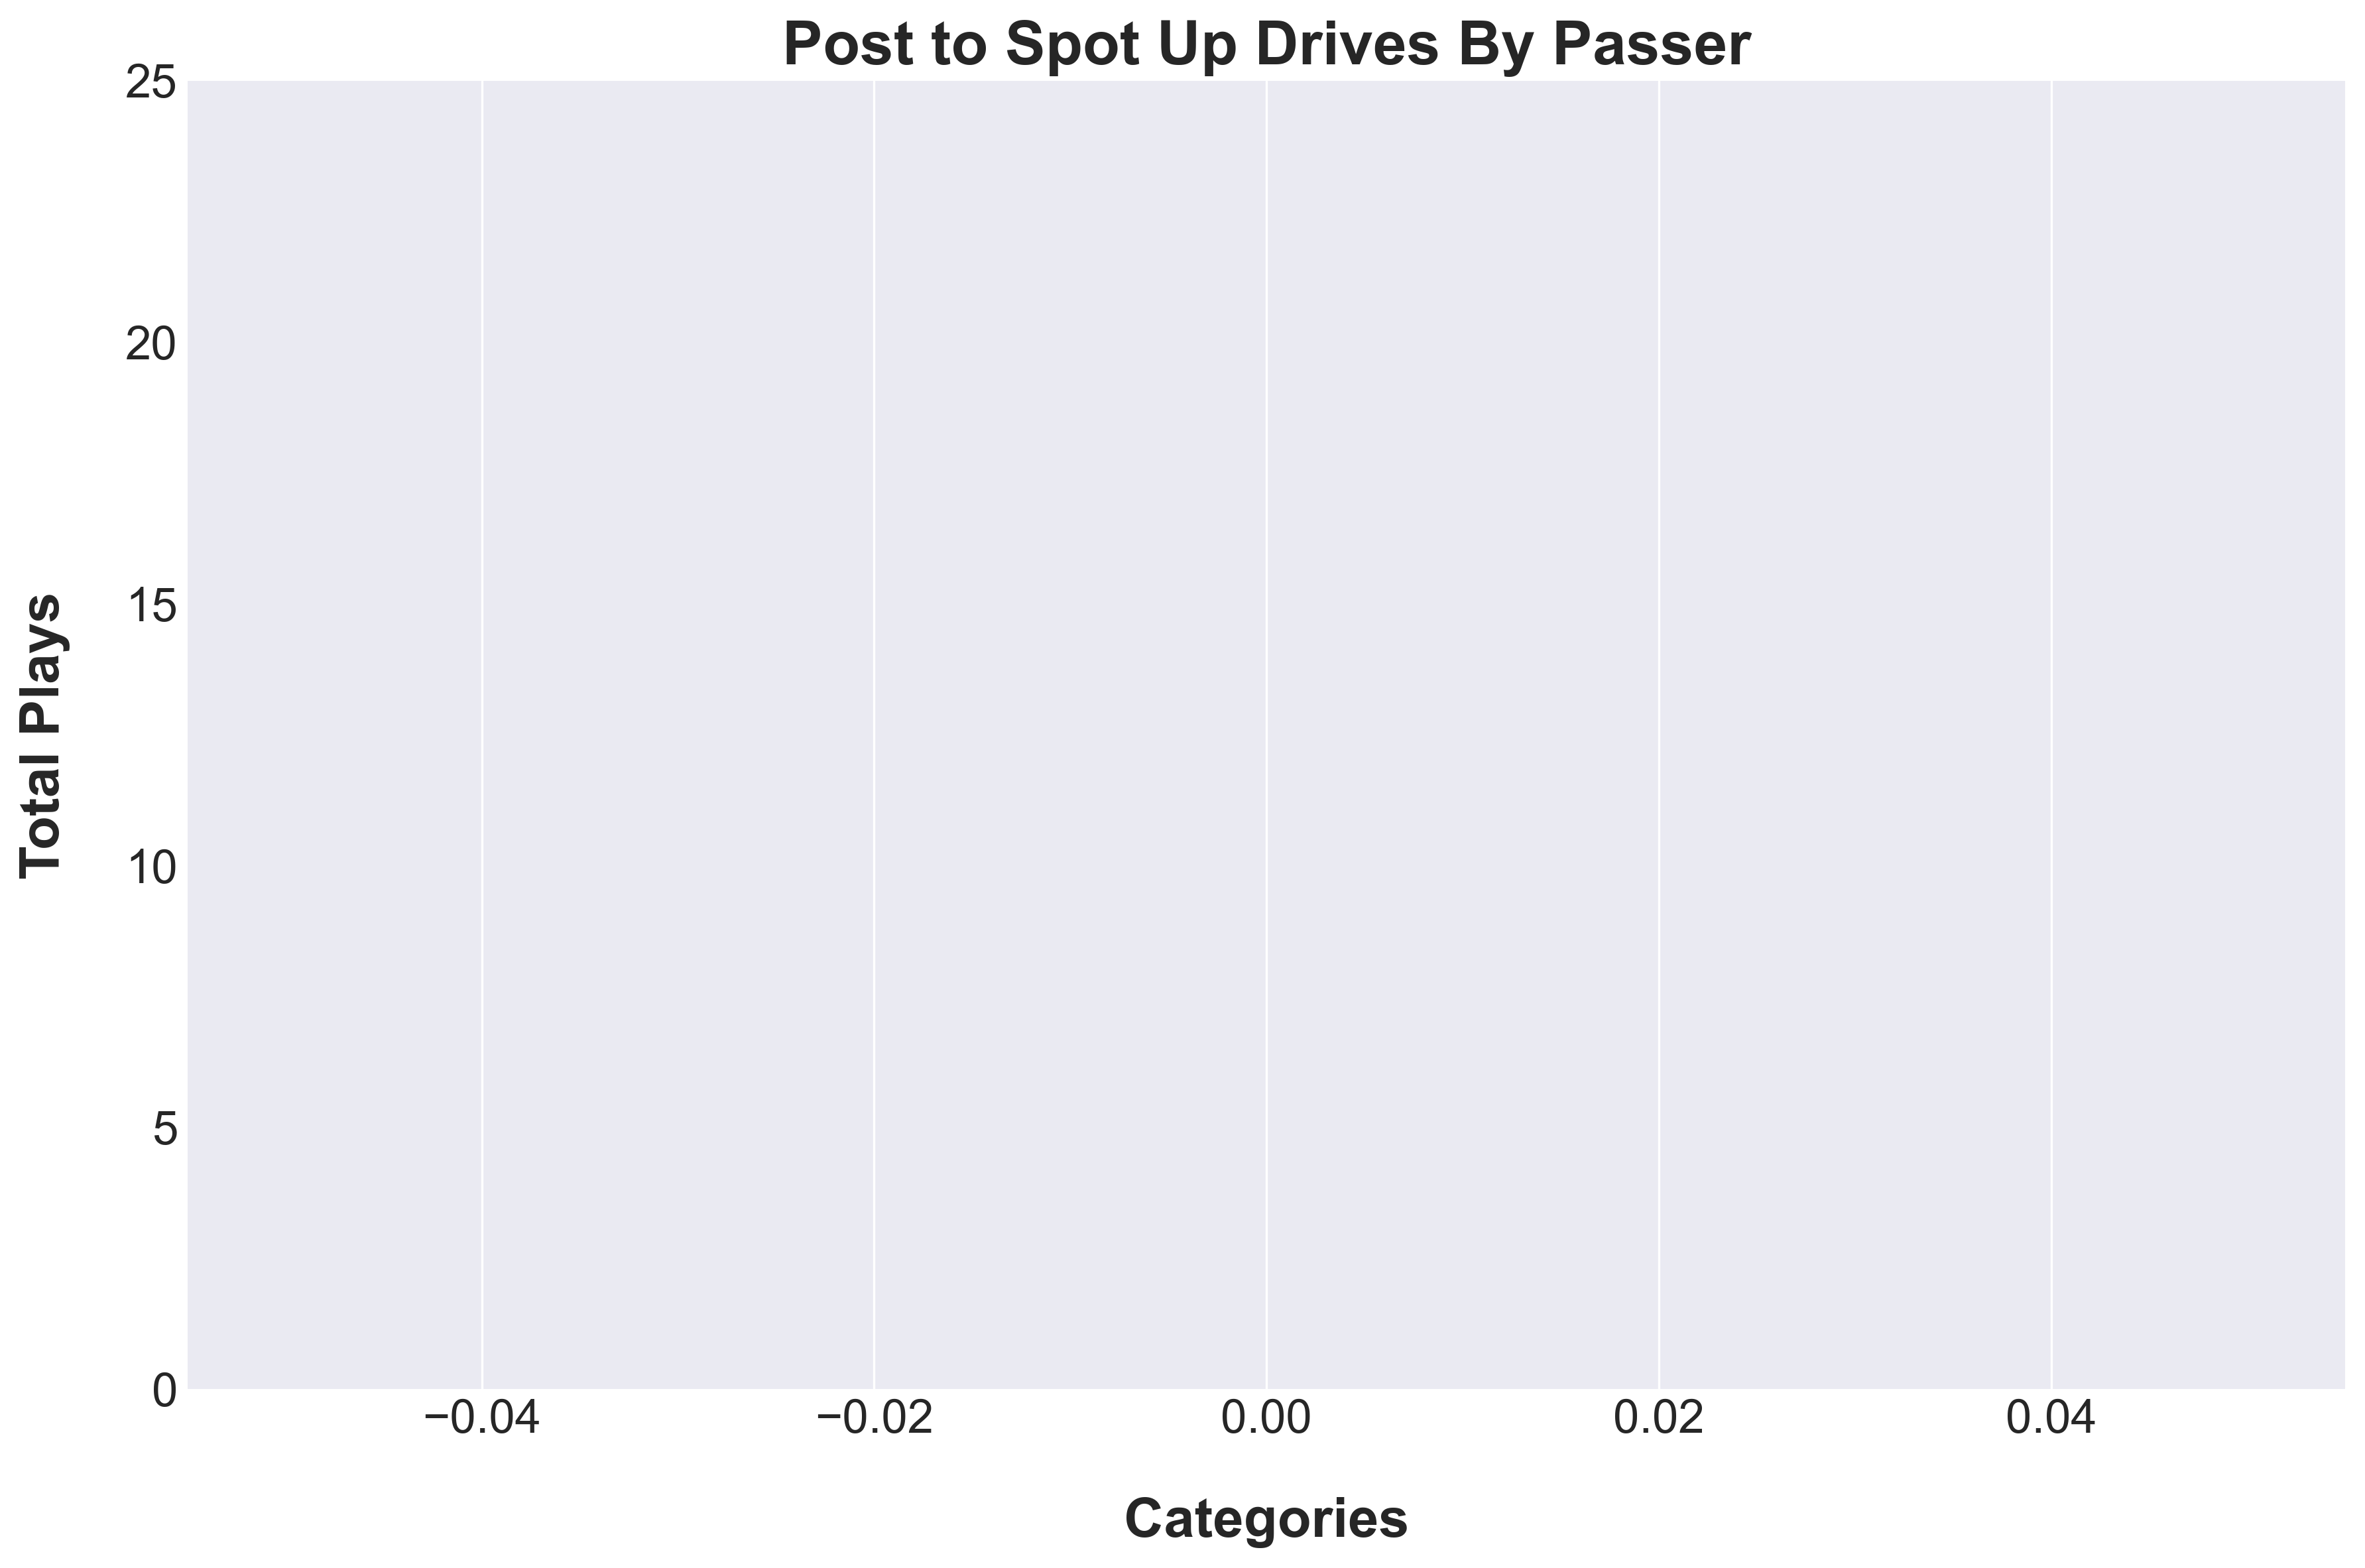
\includegraphics[width=\textwidth, height=.14\textheight]{images/SpotUp_PostDrivesPlayer_Freq.png} % Adjust the width of the image to fit
    \end{minipage}
\end{table}

\vspace{-1em} % Add vertical space before the line (optional)
\vspace{-1em} % Add vertical space after the line (optional)

% Iso -> Drive Stats by Passer
\begin{table}[H]
    \raisebox{3em}{ % Adjust this value to shift the tables vertically
    \begin{minipage}[t]{0.6\textwidth} % Left side (table) takes 85% of the width
        \flushleft
        \centering % Centering the title and the table
        \text{Iso - Drive Stats by Passer} % Title above the table in bold
        \vskip .25em % Adds vertical space between title and table
        \scalebox{.6}{ % Scale the entire table down by half
            \renewcommand{\arraystretch}{1.4} % Adjust the number to increase or decrease row spacing
            \begin{tabular}{
            >{\centering\arraybackslash}p{1.75cm} 
            >{\centering\arraybackslash}p{.75cm} 
            >{\centering\arraybackslash}p{.75cm} 
            >{\centering\arraybackslash}p{.75cm} 
            >{\centering\arraybackslash}p{.75cm}
            >{\centering\arraybackslash}p{.75cm} 
            >{\centering\arraybackslash}p{.75cm} 
            >{\centering\arraybackslash}p{.75cm} 
            >{\centering\arraybackslash}p{.75cm}
            >{\centering\arraybackslash}p{.75cm} 
            >{\centering\arraybackslash}p{.75cm}
            >{\centering\arraybackslash}p{.75cm}
            >{\centering\arraybackslash}p{.75cm} 
            >{\centering\arraybackslash}p{.75cm}}% Adjust column widths
            \toprule
            {\scriptsize \textbf{Player}} &
            {\scriptsize \textbf{Plays}} &
            {\scriptsize \textbf{3PA}} &
            {\scriptsize \textbf{3PM}} &
            {\scriptsize \textbf{3P\%}} & 
            {\scriptsize \textbf{2PA}} & 
            {\scriptsize \textbf{2PM}} & 
            {\scriptsize \textbf{2P\%}} & 
            {\scriptsize \textbf{MiA}} & 
            {\scriptsize \textbf{MiM}} &
            {\scriptsize \textbf{Mi\%}} &
            {\scriptsize \textbf{EFG\%}} &
            {\scriptsize \textbf{TO}} &
            {\scriptsize \textbf{Foul}} \\
            \midrule
            
                
            
                
            
                
            
                
            
                
                    
                
            
                
            
                
            
                
            
                
            
                
            
                
            
                
            
                
            
                
            
                
            
                
            
                
            
                
            
                
            
                
            
                
            
                
            

            \bottomrule
        \end{tabular}
        } % End of \scalebox
    \end{minipage}
    } % End of raisebox, closing the adjustment
    \hfill % This adds some flexible space between the table and the image
    \begin{minipage}[c]{0.35\textwidth} % Right side (image) takes 10% of the width
        \flushright
        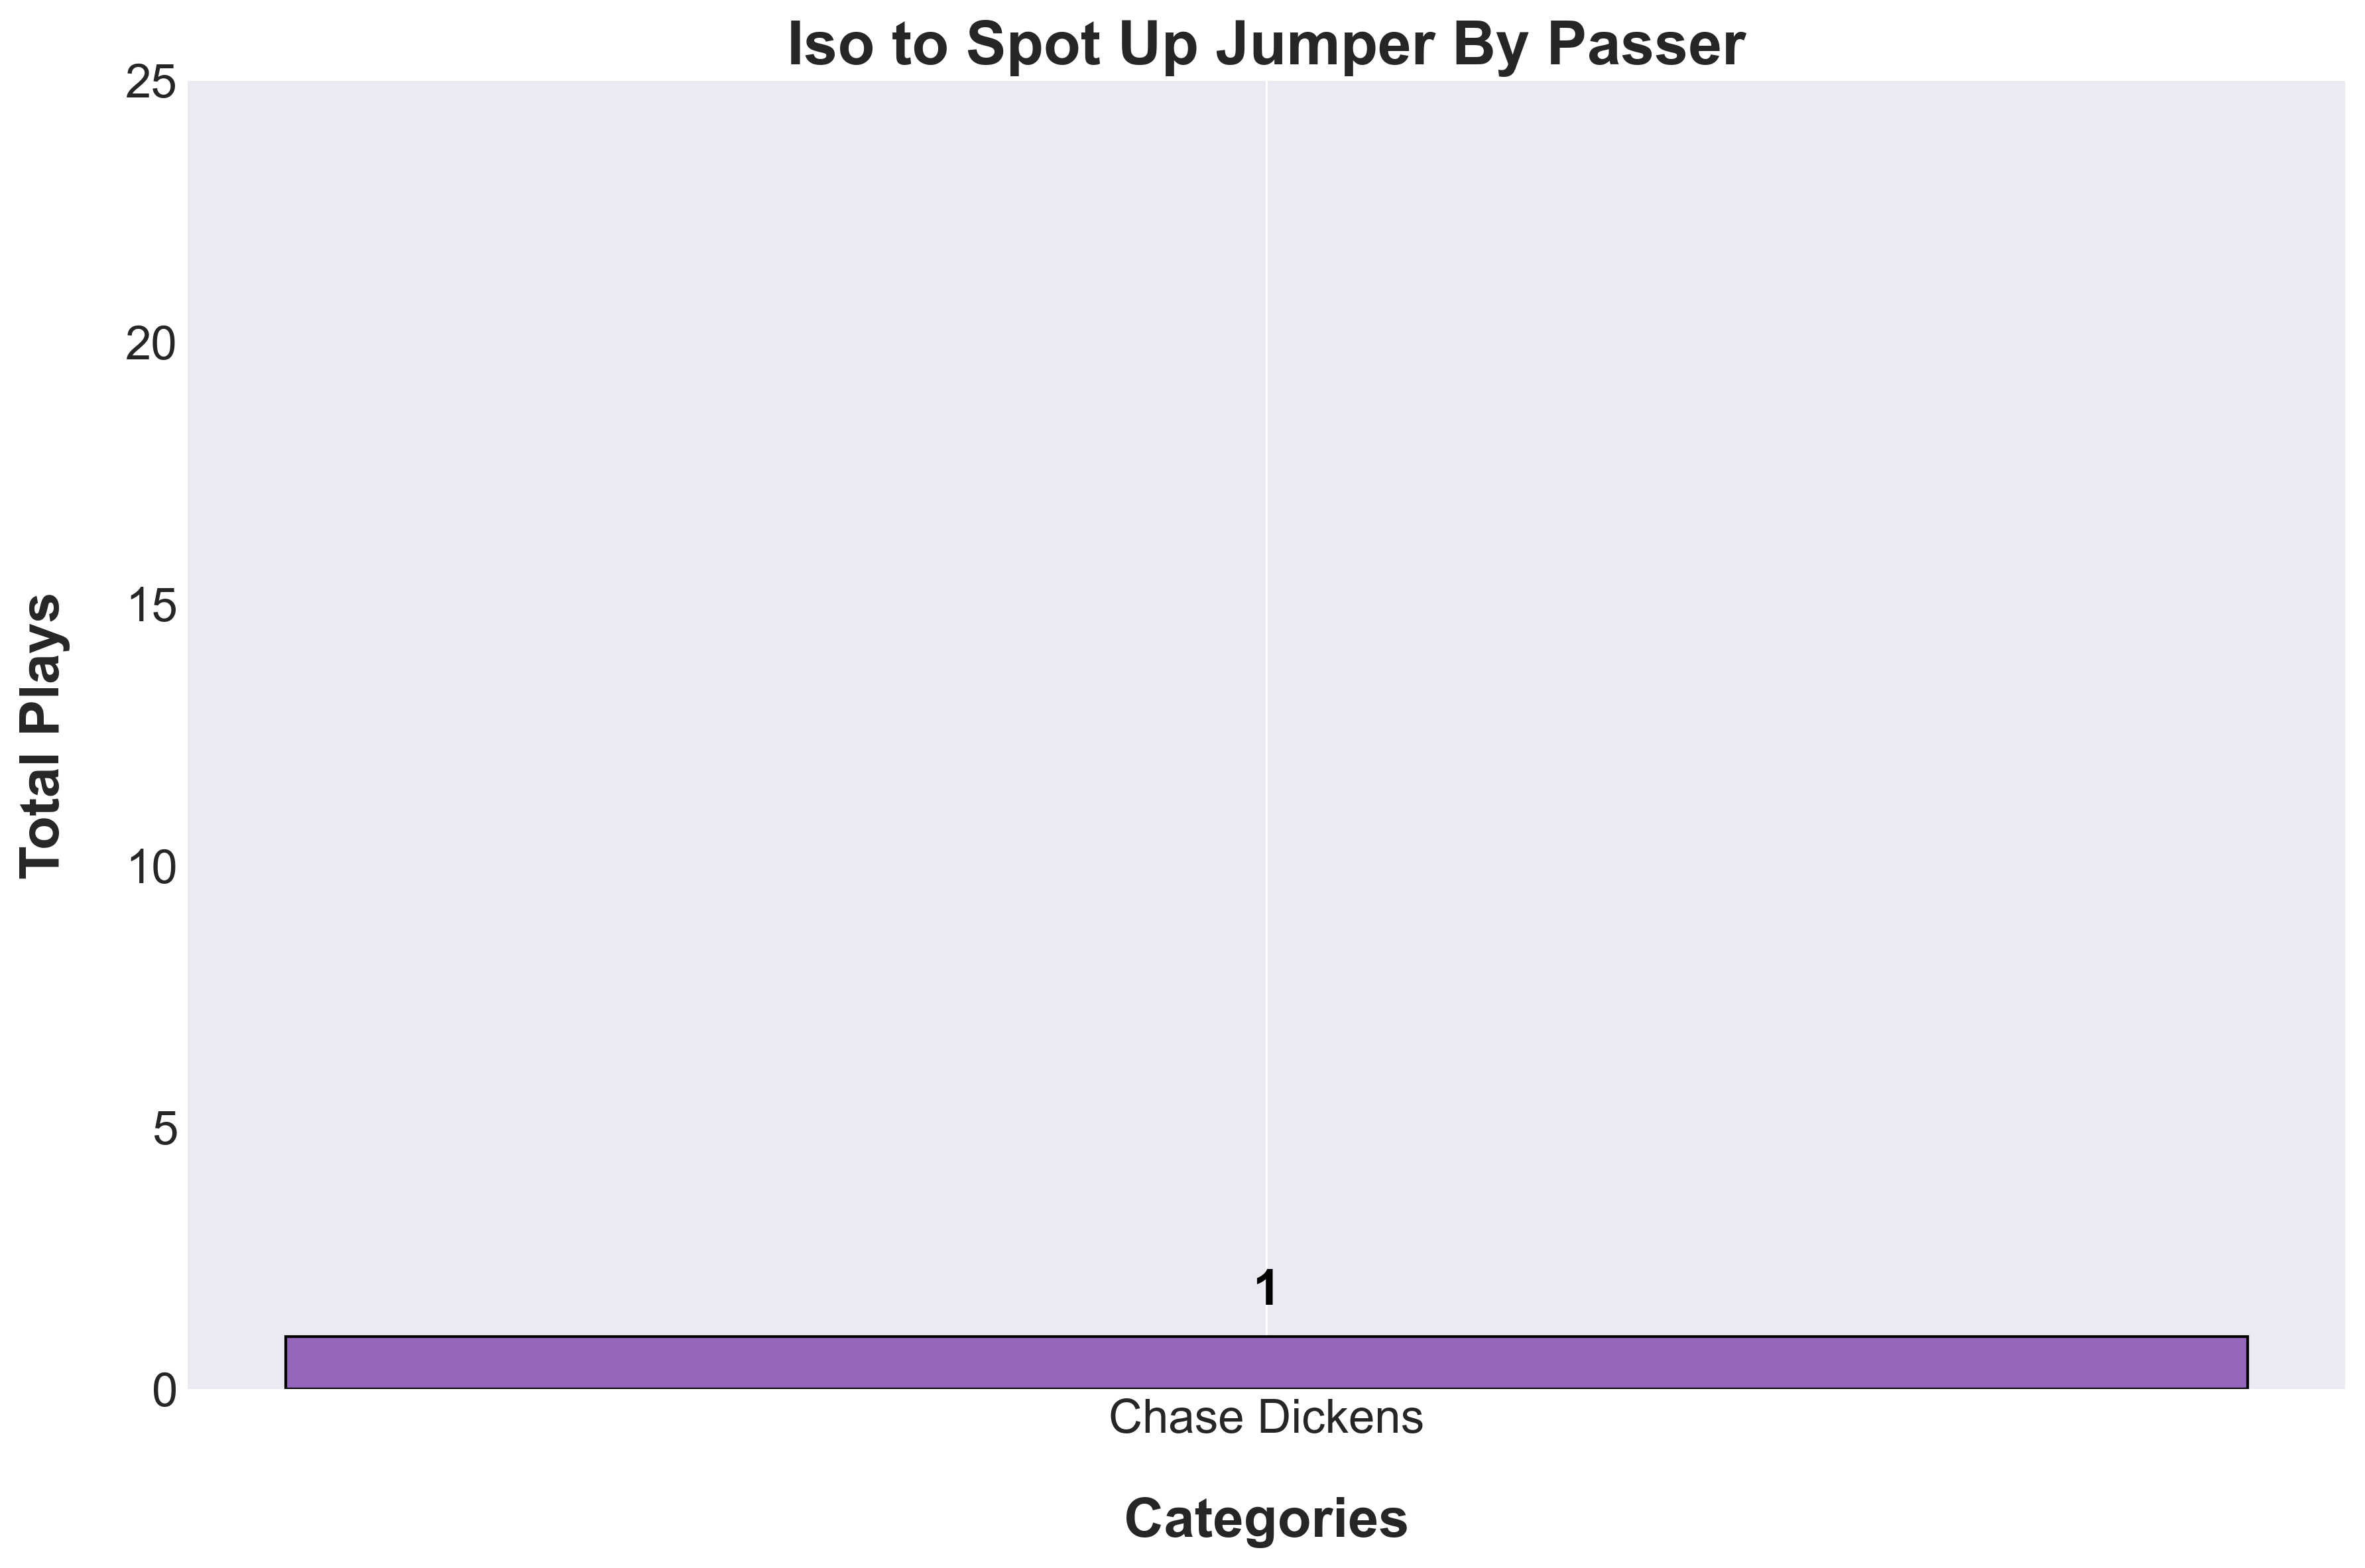
\includegraphics[width=\textwidth, height=.14\textheight]{images/SpotUp_IsoShotsPlayer_Freq.png} % Adjust the width of the image to fit
    \end{minipage}
\end{table}

\vspace{-1em} % Add vertical space before the line (optional)
\vspace{-1em} % Add vertical space after the line (optional)

% PNR -> Drive Stats by Passer
\begin{table}[H]
    \raisebox{3em}{ % Adjust this value to shift the tables vertically
    \begin{minipage}[t]{0.6\textwidth} % Left side (table) takes 85% of the width
        \flushleft
        \centering % Centering the title and the table
        \text{PNR - Drive Stats by Passer} % Title above the table in bold
        \vskip .25em % Adds vertical space between title and table
        \scalebox{.6}{ % Scale the entire table down by half
            \renewcommand{\arraystretch}{1.4} % Adjust the number to increase or decrease row spacing
            \begin{tabular}{
            >{\centering\arraybackslash}p{1.75cm} 
            >{\centering\arraybackslash}p{.75cm} 
            >{\centering\arraybackslash}p{.75cm} 
            >{\centering\arraybackslash}p{.75cm} 
            >{\centering\arraybackslash}p{.75cm}
            >{\centering\arraybackslash}p{.75cm} 
            >{\centering\arraybackslash}p{.75cm} 
            >{\centering\arraybackslash}p{.75cm} 
            >{\centering\arraybackslash}p{.75cm}
            >{\centering\arraybackslash}p{.75cm} 
            >{\centering\arraybackslash}p{.75cm}
            >{\centering\arraybackslash}p{.75cm}
            >{\centering\arraybackslash}p{.75cm} 
            >{\centering\arraybackslash}p{.75cm}}% Adjust column widths
            \toprule
            {\scriptsize \textbf{Player}} &
            {\scriptsize \textbf{Plays}} &
            {\scriptsize \textbf{3PA}} &
            {\scriptsize \textbf{3PM}} &
            {\scriptsize \textbf{3P\%}} & 
            {\scriptsize \textbf{2PA}} & 
            {\scriptsize \textbf{2PM}} & 
            {\scriptsize \textbf{2P\%}} & 
            {\scriptsize \textbf{MiA}} & 
            {\scriptsize \textbf{MiM}} &
            {\scriptsize \textbf{Mi\%}} &
            {\scriptsize \textbf{EFG\%}} &
            {\scriptsize \textbf{TO}} &
            {\scriptsize \textbf{Foul}} \\
            \midrule
            
                
            
                
            
                
            
                
            
                
            
                
            
                
            
                
            
                
                    
                        Brock Bowen & 
                        2 & 
                        0 & 
                        0 & 
                        - & 
                        1 & 
                        1 & 
                        - & 
                        0 & 
                        0 & 
                        - & 
                        - & 
                        1 & 
                        0 \\
                    
                        Brody Brown & 
                        1 & 
                        0 & 
                        0 & 
                        - & 
                        0 & 
                        0 & 
                        - & 
                        0 & 
                        0 & 
                        - & 
                        - & 
                        1 & 
                        0 \\
                    
                        Mark Osime & 
                        1 & 
                        0 & 
                        0 & 
                        - & 
                        1 & 
                        0 & 
                        - & 
                        0 & 
                        0 & 
                        - & 
                        - & 
                        0 & 
                        0 \\
                    
                
            
                
            
                
            
                
            
                
            
                
            
                
            
                
            
                
            
                
            
                
            
                
            
                
            
                
            

            \bottomrule
        \end{tabular}
        } % End of \scalebox
    \end{minipage}
    } % End of raisebox, closing the adjustment
    \hfill % This adds some flexible space between the table and the image
    \begin{minipage}[c]{0.35\textwidth} % Right side (image) takes 10% of the width
        \flushright
        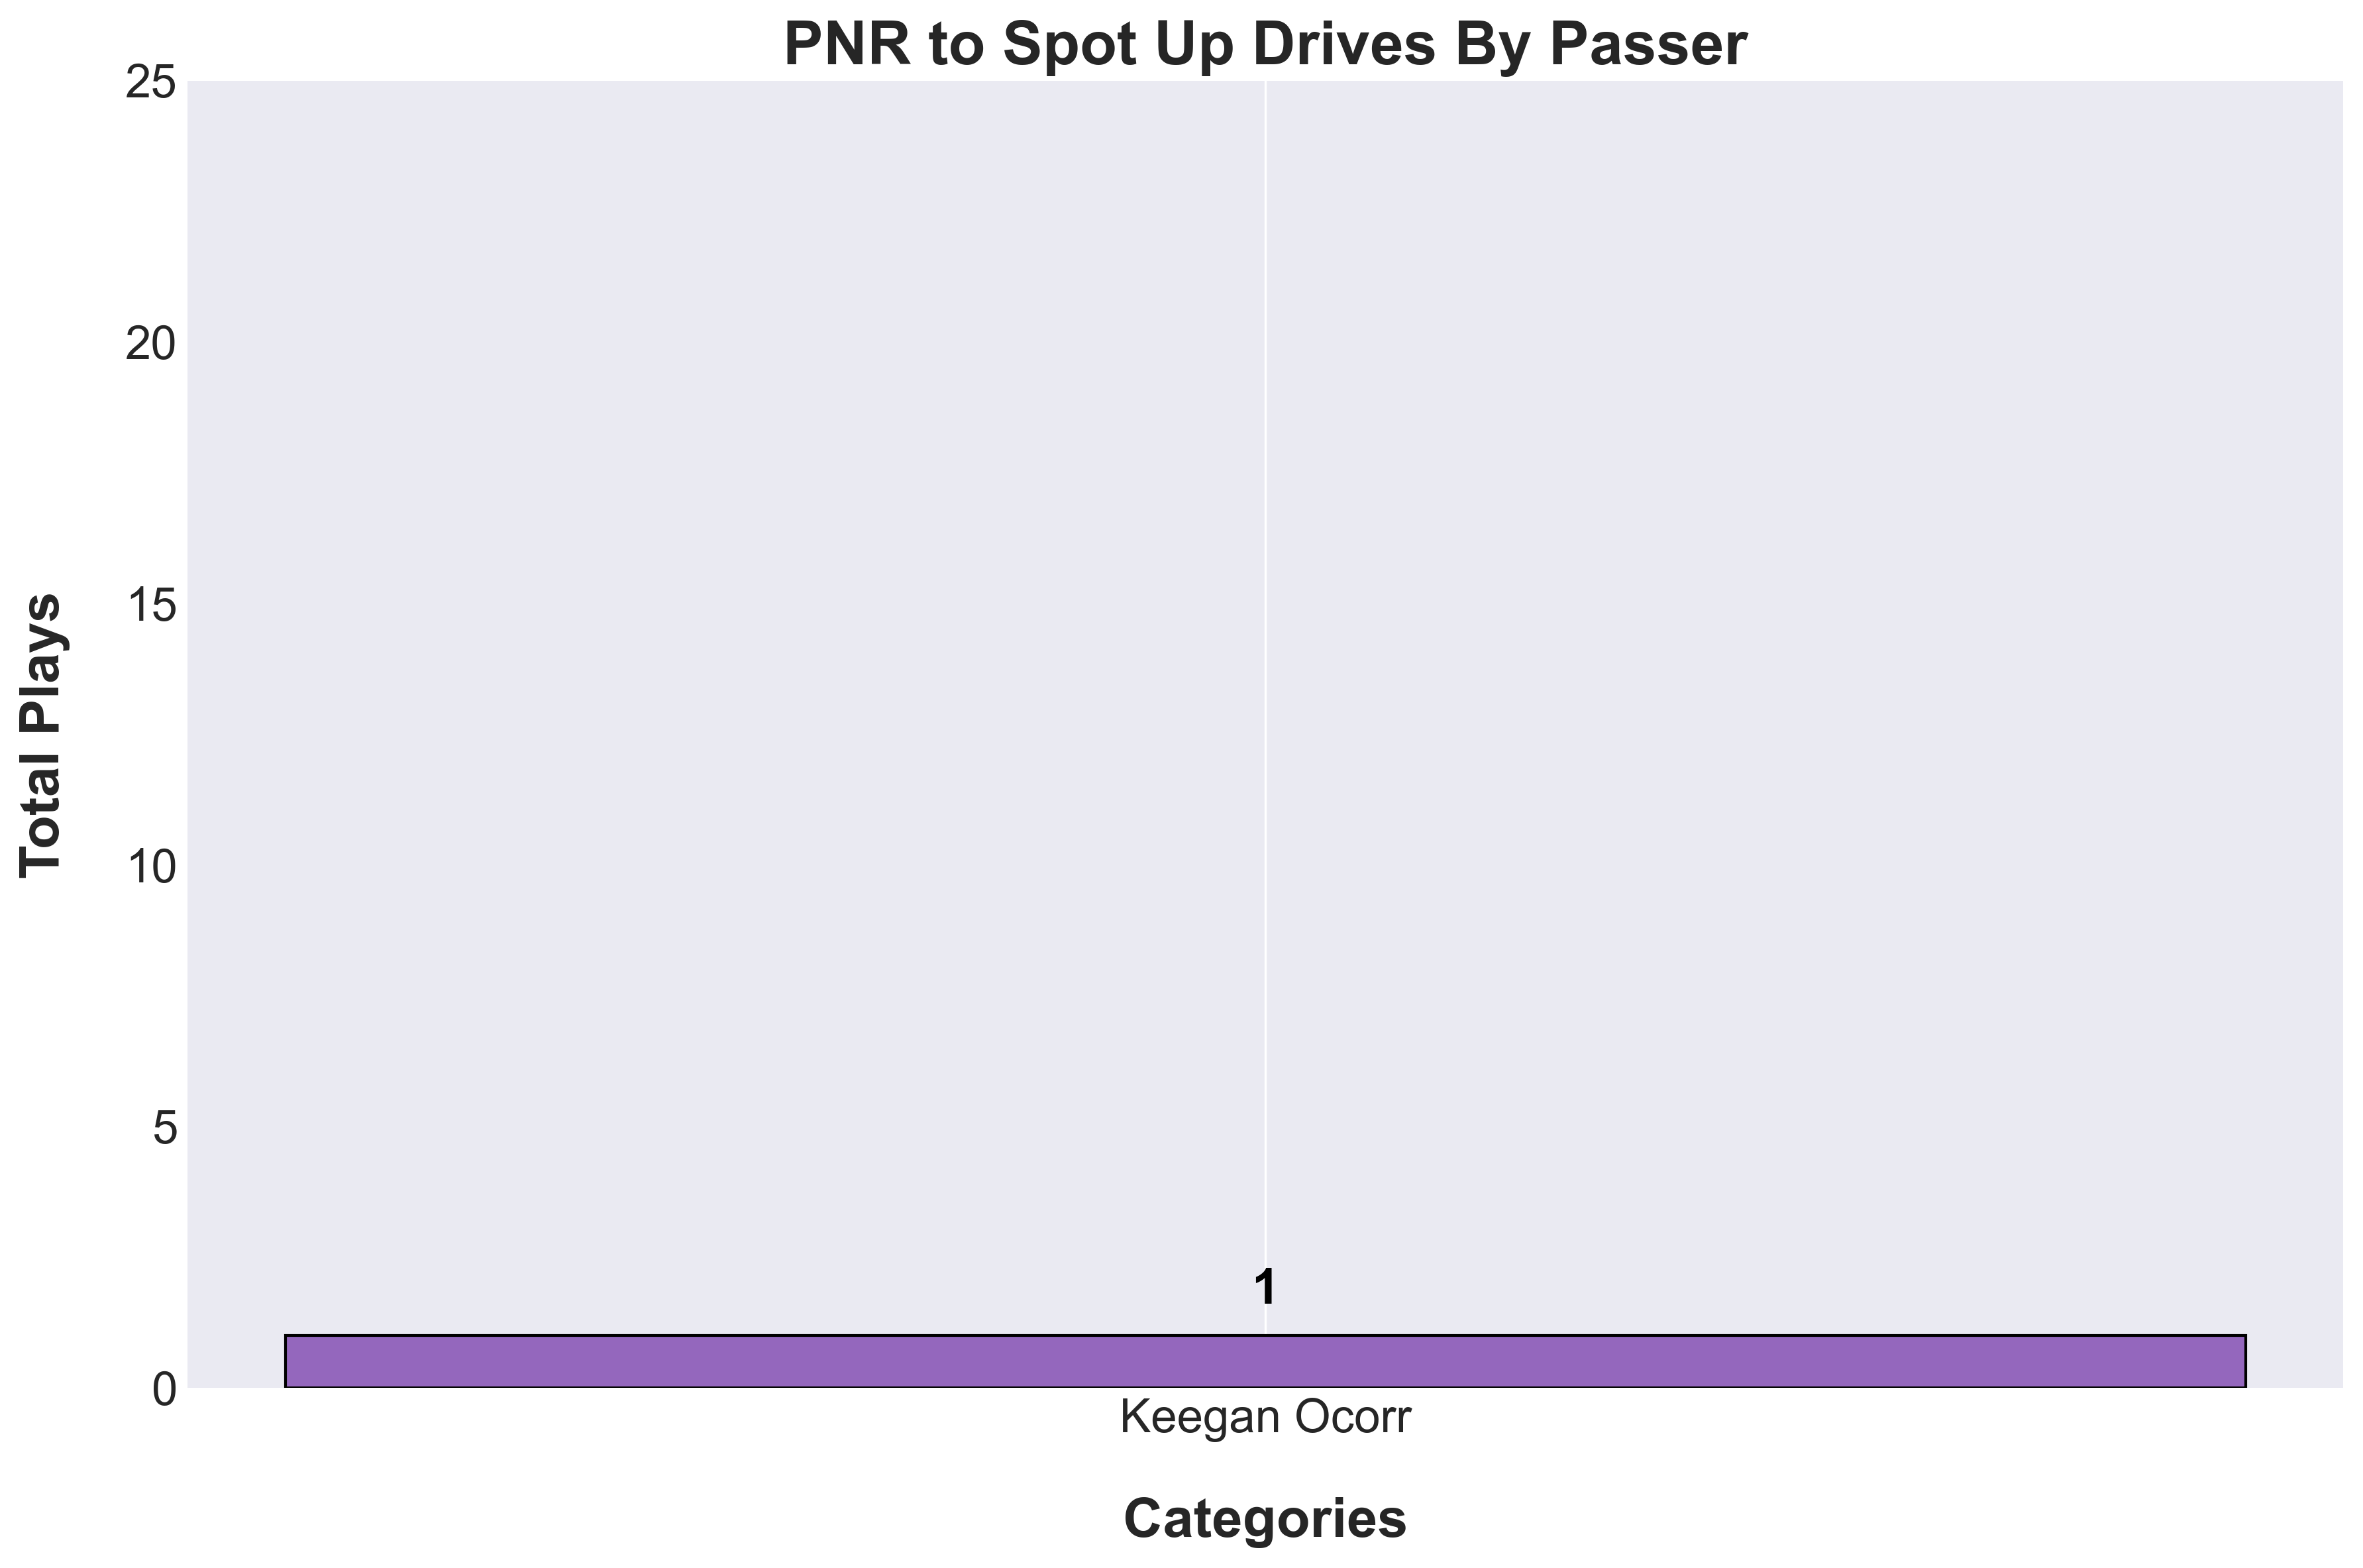
\includegraphics[width=\textwidth, height=.14\textheight]{images/SpotUp_PnrDrivesPlayer_Freq.png} % Adjust the width of the image to fit
    \end{minipage}
\end{table}

\vspace{-1em} % Add vertical space before the line (optional)
\hrule height 1pt width 1\textwidth % Adjust height and width
\vspace{1em} % Add vertical space after the line (optional)
\clearpage











% ----------------------
% Off Screen Visuals and Insights Section
% ----------------------
\subsection{Off Screens}
\vspace{1.25em} % Add vertical space before the line (optional)
\textbf{Key Notes on Off Screen Tendencies}
\vspace{0.5em} % Add space between the title and the itemized list

\begin{itemize}
    \item Off Screens make up x\% of players offensive load
    \vspace{0.3em} % Add space between the title and the itemized list
    \item Player is more efficient when coming off his left shoulder and get shots off of his left shoulder x\% of the time.
\end{itemize}

\vspace{1em} % Add vertical space before the line (optional)
\hrule height 1pt width 1\textwidth % Adjust height and width
\vspace{0em} % Add vertical space after the line (optional)

\subsubsection{Off Screen Shot Statistics}

% All Off Screen Statistics Table w/ room for insights
\begin{table}[H]
    \centering
    \begin{minipage}[t]{0.6\textwidth} % Left side (table) takes 85% of the width
        %\flushright
        \centering % Centering the title and the table
        \text{Total Off Screen Shot Statistics} % Title above the table in bold
        \vskip .25em % Adds vertical space between title and table
        \scalebox{.85}{ % Scale the entire table down by half
            \scriptsize % Reduce the font size
            \begin{tabular}{
            >{\centering\arraybackslash}p{.75cm} 
            >{\centering\arraybackslash}p{.5cm} 
            >{\centering\arraybackslash}p{.5cm} 
            >{\centering\arraybackslash}p{.5cm}
            >{\centering\arraybackslash}p{.5cm} 
            >{\centering\arraybackslash}p{.5cm} 
            >{\centering\arraybackslash}p{.5cm} 
            >{\centering\arraybackslash}p{.5cm}
            >{\centering\arraybackslash}p{.5cm} 
            >{\centering\arraybackslash}p{.5cm}
            >{\centering\arraybackslash}p{.75cm}
            >{\centering\arraybackslash}p{.5cm} 
            >{\centering\arraybackslash}p{.5cm}}% Adjust column widths
            \toprule
            \textbf{Plays} &
            \textbf{3PA} &
            \textbf{3PM} &
            \textbf{3P\%} & 
            \textbf{2PA} & 
            \textbf{2PM} & 
            \textbf{2P\%} & 
            \textbf{MiA} & 
            \textbf{MiM} &
            \textbf{Mi\%} &
            \textbf{EFG\%} &
            \textbf{TO} &
            \textbf{Foul} \\
            \midrule
            
                
                    13 & 3 & 0 &
                    - & 
                    9 & 4 &
                    - &
                    2 & 0 &
                    - &
                    - &
                    1 & 0 \\
                
            
                
            
                
            
                
            
                
            
                
            
                
            
                
            
                
            
                
            
                
            
                
            
                
            
                
            


            \bottomrule
            \end{tabular}
        }
    \end{minipage}
\end{table}

\vspace{0em} % Add vertical space before the line (optional)
%\hrule height 1pt width 1\textwidth % Adjust height and width
\vspace{-1em} % Add vertical space after the line (optional)

% Off Screen Stats for shooting off Left vs Right Shoulder
\begin{table}[H]
    \raisebox{3em}{ % Adjust this value to shift the tables vertically
    \begin{minipage}[t]{0.6\textwidth} % Left side (table) takes 85% of the width
        \flushleft
        \centering % Centering the title and the table
        \text{Shots Running Off Specific Shoulder Statistics} % Title above the table in bold
        \vskip .25em % Adds vertical space between title and table
        \scalebox{.6}{ % Scale the entire table down by half
            \renewcommand{\arraystretch}{1.4} % Adjust the number to increase or decrease row spacing
            \begin{tabular}{
            >{\centering\arraybackslash}p{1.75cm} 
            >{\centering\arraybackslash}p{.75cm} 
            >{\centering\arraybackslash}p{.75cm} 
            >{\centering\arraybackslash}p{.75cm} 
            >{\centering\arraybackslash}p{.75cm}
            >{\centering\arraybackslash}p{.75cm} 
            >{\centering\arraybackslash}p{.75cm} 
            >{\centering\arraybackslash}p{.75cm} 
            >{\centering\arraybackslash}p{.75cm}
            >{\centering\arraybackslash}p{.75cm} 
            >{\centering\arraybackslash}p{.75cm}
            >{\centering\arraybackslash}p{.75cm}
            >{\centering\arraybackslash}p{.75cm} 
            >{\centering\arraybackslash}p{.75cm}}% Adjust column widths
            \toprule
            {\scriptsize \textbf{PlayType}} &
            {\scriptsize \textbf{Plays}} &
            {\scriptsize \textbf{3PA}} &
            {\scriptsize \textbf{3PM}} &
            {\scriptsize \textbf{3P\%}} & 
            {\scriptsize \textbf{2PA}} & 
            {\scriptsize \textbf{2PM}} & 
            {\scriptsize \textbf{2P\%}} & 
            {\scriptsize \textbf{MiA}} & 
            {\scriptsize \textbf{MiM}} &
            {\scriptsize \textbf{Mi\%}} &
            {\scriptsize \textbf{EFG\%}} &
            {\scriptsize \textbf{TO}} &
            {\scriptsize \textbf{Foul}} \\
            \midrule
            
                
            
                
            
                
                    Left & 3 & 0 & 0 &
                    - & 
                    3 & 1 &
                    - &
                    1 & 0 &
                    - &
                    - &
                    0 & 0 \\
                
            
                
                    Right & 10 & 3 & 0 &
                    - & 
                    6 & 3 &
                    - &
                    1 & 0 &
                    - &
                    - &
                    1 & 0 \\
                
            
                
            
                
            
                
            
                
            
                
            
                
            
                
            
                
            
                
            
                
            

            \bottomrule
        \end{tabular}
        } % End of \scalebox
    \end{minipage}
    } % End of raisebox, closing the adjustment
    \hfill % This adds some flexible space between the table and the image
    \begin{minipage}[c]{0.35\textwidth} % Right side (image) takes 10% of the width
        \flushright
        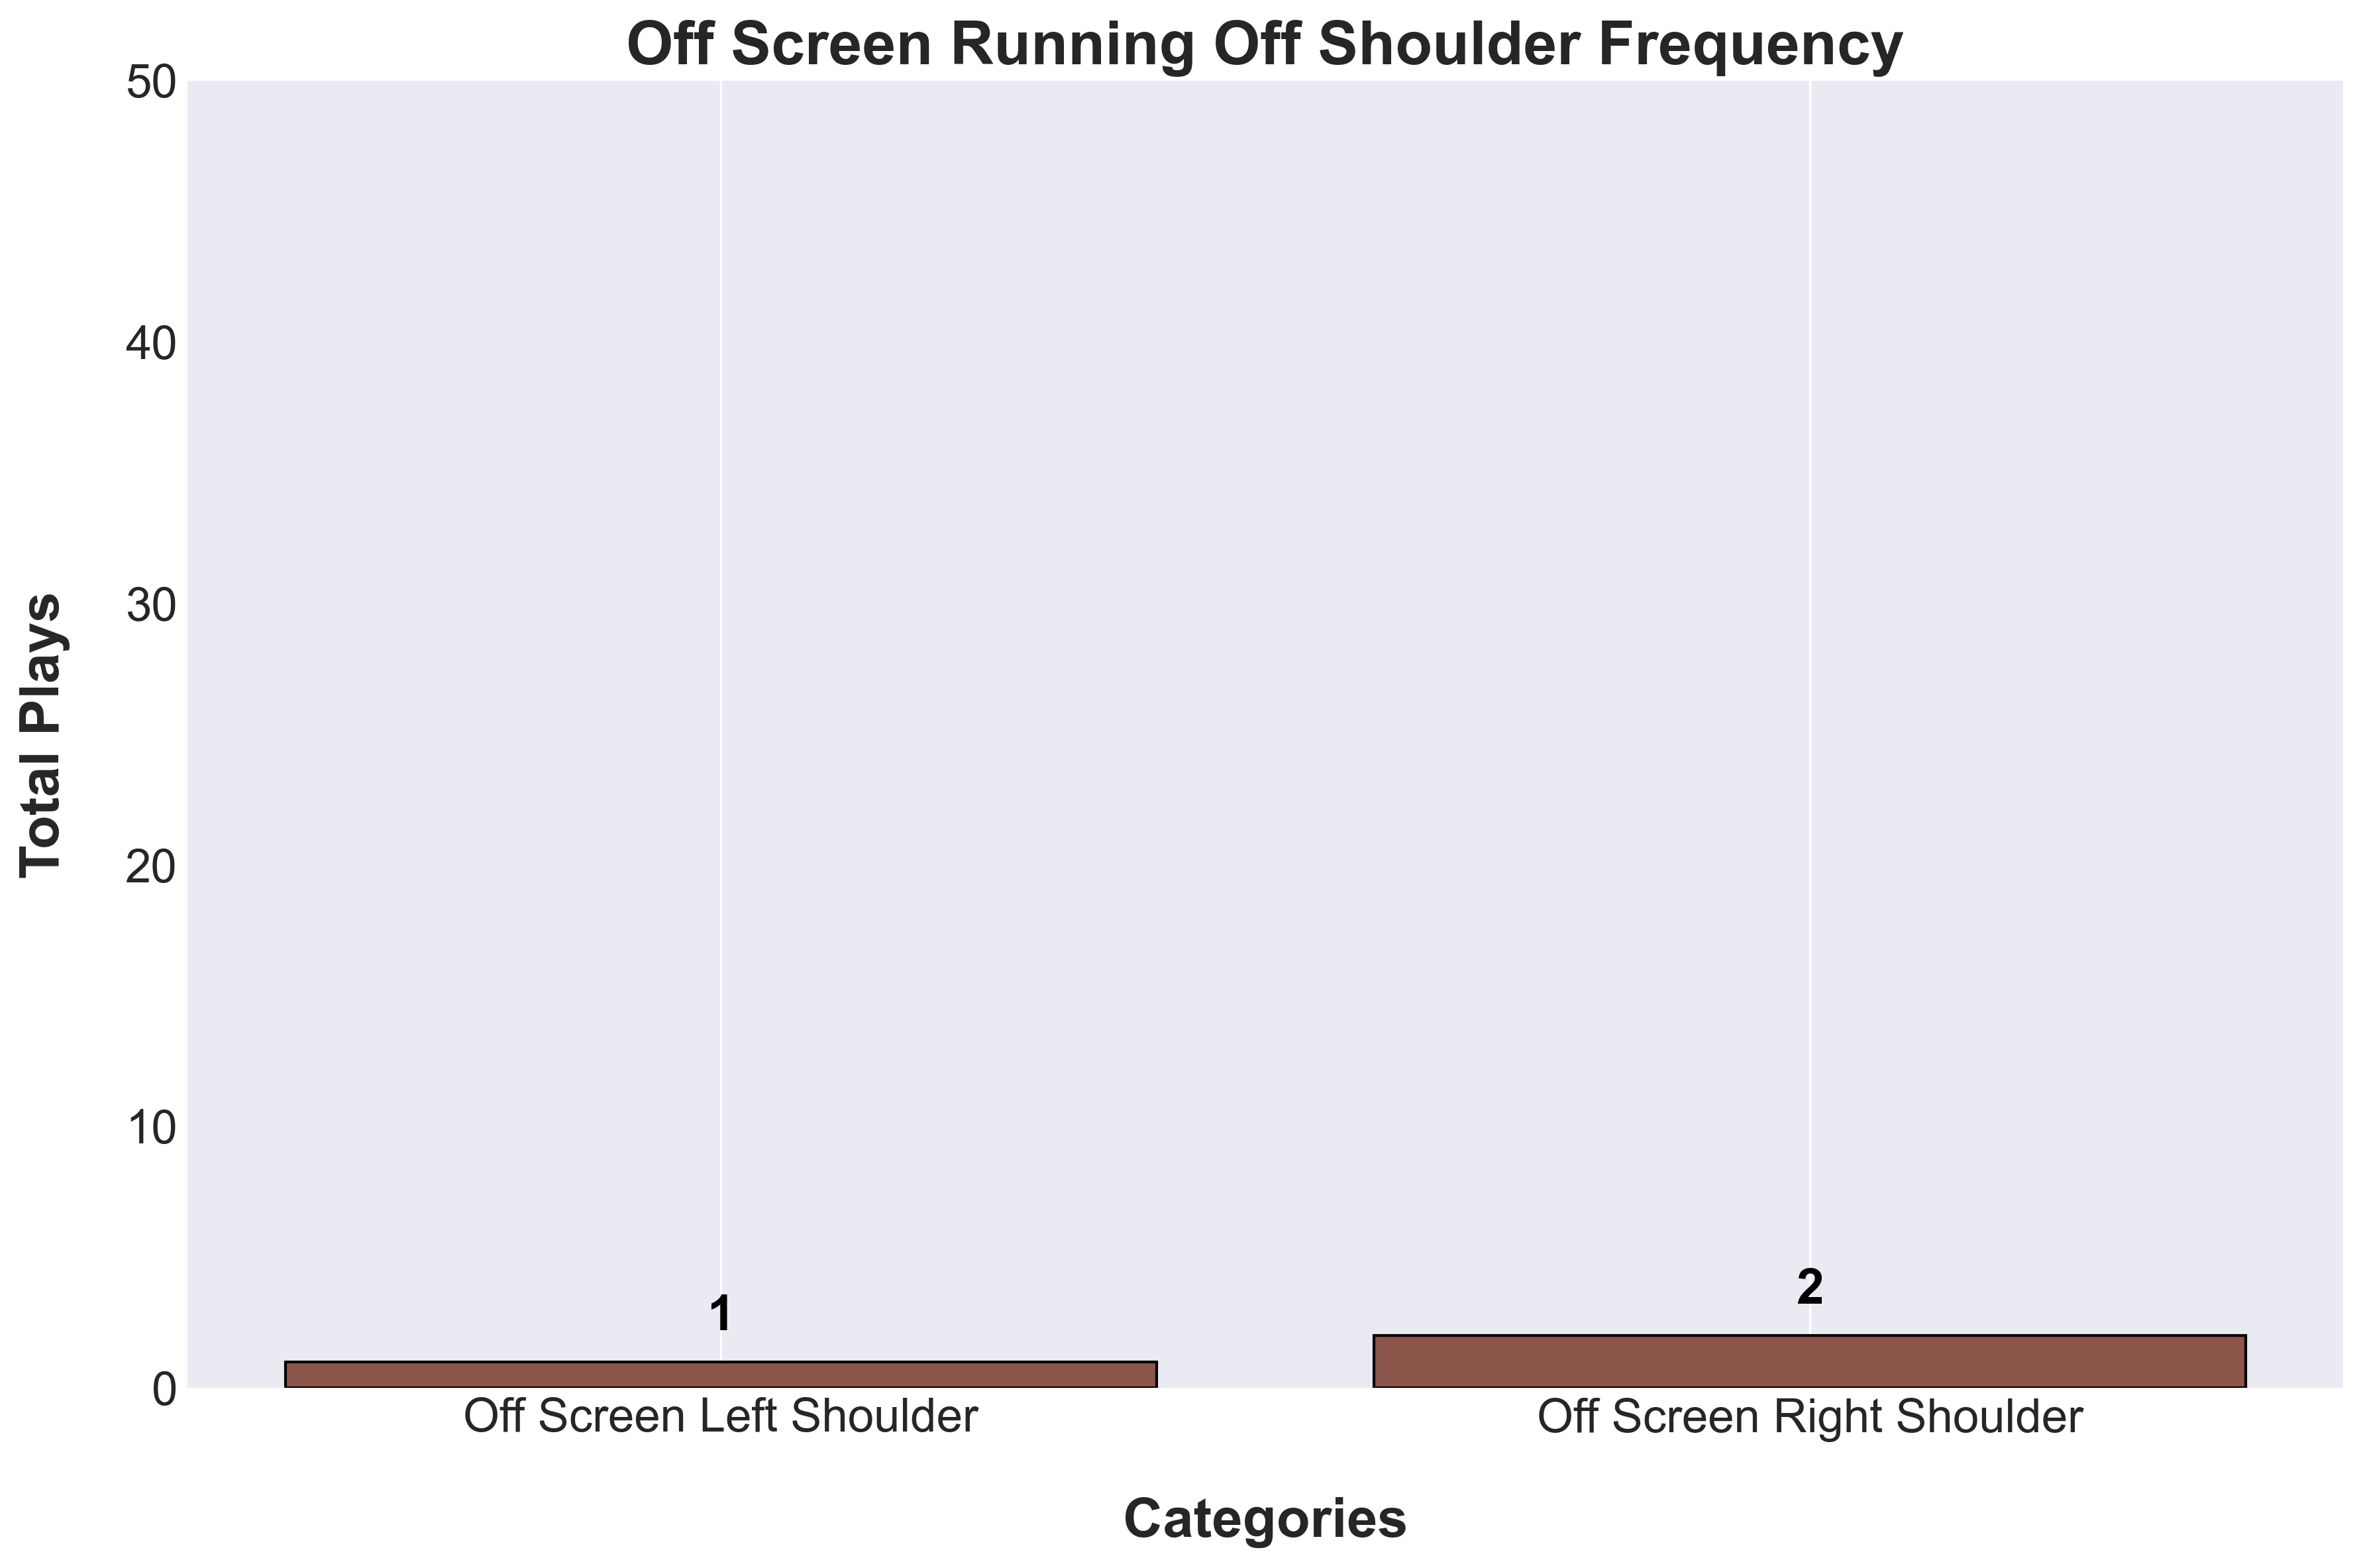
\includegraphics[width=\textwidth, height=.14\textheight]{images/OffScreen_Shoulder_Freq.png} % Adjust the width of the image to fit
    \end{minipage}
\end{table}

\vspace{-1em} % Add vertical space before the line (optional)
%\hrule height 1pt width 1\textwidth % Adjust height and width
\vspace{-1em} % Add vertical space after the line (optional)

% Off Screen Type Statistics
\begin{table}[H]
    \raisebox{3.5em}{ % Adjust this value to shift the tables vertically
    \begin{minipage}[t]{0.6\textwidth} % Left side (table) takes 85% of the width
        \flushleft
        \centering % Centering the title and the table
        \text{Off Screen Type Statistics} % Title above the table in bold
        \vskip .25em % Adds vertical space between title and table
        \scalebox{.6}{ % Scale the entire table down by half
            \renewcommand{\arraystretch}{1.4} % Adjust the number to increase or decrease row spacing
            \begin{tabular}{
            >{\centering\arraybackslash}p{1.75cm} 
            >{\centering\arraybackslash}p{.75cm} 
            >{\centering\arraybackslash}p{.75cm} 
            >{\centering\arraybackslash}p{.75cm} 
            >{\centering\arraybackslash}p{.75cm}
            >{\centering\arraybackslash}p{.75cm} 
            >{\centering\arraybackslash}p{.75cm} 
            >{\centering\arraybackslash}p{.75cm} 
            >{\centering\arraybackslash}p{.75cm}
            >{\centering\arraybackslash}p{.75cm} 
            >{\centering\arraybackslash}p{.75cm}
            >{\centering\arraybackslash}p{.75cm}
            >{\centering\arraybackslash}p{.75cm} 
            >{\centering\arraybackslash}p{.75cm}}% Adjust column widths
            \toprule
            {\scriptsize \textbf{PlayType}} &
            {\scriptsize \textbf{Plays}} &
            {\scriptsize \textbf{3PA}} &
            {\scriptsize \textbf{3PM}} &
            {\scriptsize \textbf{3P\%}} & 
            {\scriptsize \textbf{2PA}} & 
            {\scriptsize \textbf{2PM}} & 
            {\scriptsize \textbf{2P\%}} & 
            {\scriptsize \textbf{MiA}} & 
            {\scriptsize \textbf{MiM}} &
            {\scriptsize \textbf{Mi\%}} &
            {\scriptsize \textbf{EFG\%}} &
            {\scriptsize \textbf{TO}} &
            {\scriptsize \textbf{Foul}} \\
            \midrule
            
                
            
                
            
                
            
                
            
                
                    Curl &  &  &  &
                    - & 
                     &  &
                    - &
                     &  &
                    - &
                    - &
                     &  \\
                
            
                
                    Flare & 3 & 0 & 0 &
                    - & 
                    3 & 1 &
                    - &
                    1 & 0 &
                    - &
                    - &
                    0 & 0 \\
                
            
                
                    Straight & 9 & 3 & 0 &
                    - & 
                    5 & 3 &
                    - &
                    1 & 0 &
                    - &
                    - &
                    1 & 0 \\
                
            
                
                    Curl & 1 & 0 & 0 &
                    - & 
                    1 & 0 &
                    - &
                    0 & 0 &
                    - &
                    - &
                    0 & 0 \\
                
            
                
            
                
            
                
            
                
            
                
            
                
            


            \bottomrule
        \end{tabular}
        } % End of \scalebox
    \end{minipage}
    } % End of raisebox, closing the adjustment
    \hfill
    \begin{minipage}[c]{0.35\textwidth} % Right side (image) takes 10% of the width
        \flushright
        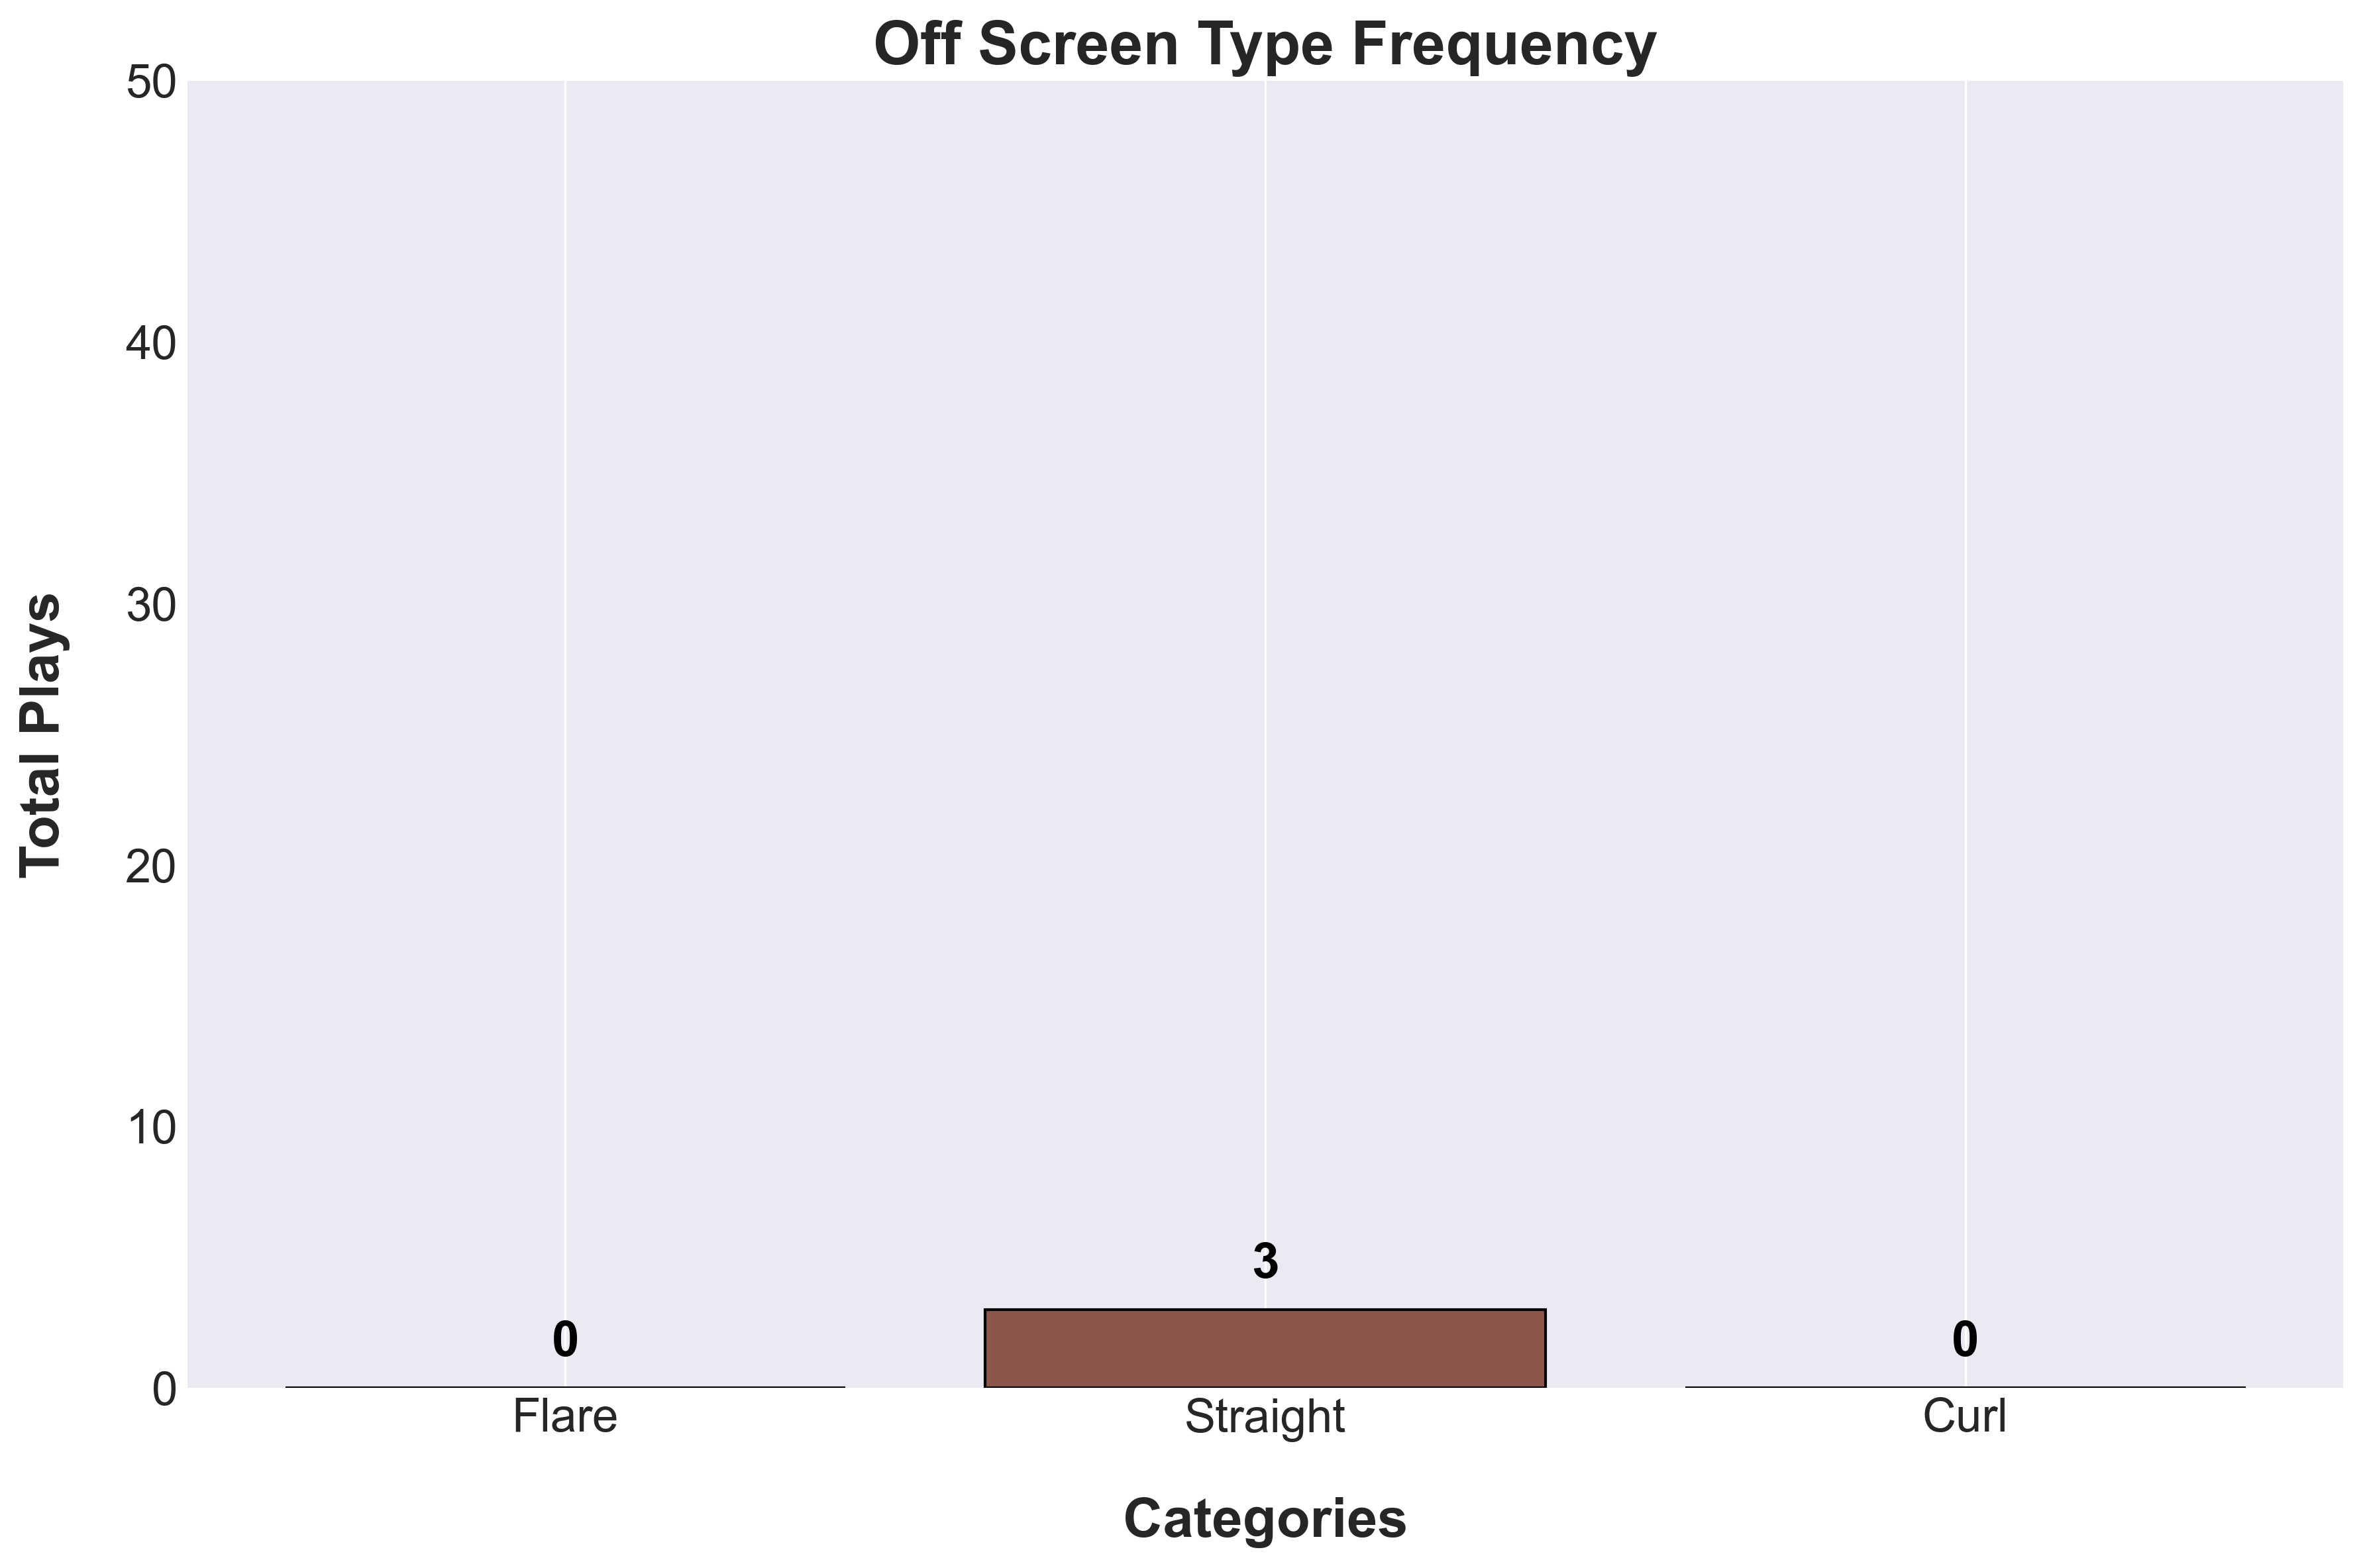
\includegraphics[width=\textwidth, height=.14\textheight]{images/OffScreen_Type_Freq.png} % Adjust the width of the image to fit
    \end{minipage}
    
\end{table}

\vspace{-1em} % Add vertical space before the line (optional)
%\hrule height 1pt width 1\textwidth % Adjust height and width
\vspace{-1em} % Add vertical space after the line (optional)

% Off Screen Stats for Combination of Shoulder and Type Stats
\begin{table}[H]
    \raisebox{4.5em}{ % Adjust this value to shift the tables vertically
    \begin{minipage}[t]{0.6\textwidth} % Left side (table) takes 85% of the width
        \flushleft
        \centering % Centering the title and the table
        \text{Off Screen Combination Statistics} % Title above the table in bold
        \vskip .25em % Adds vertical space between title and table
        \scalebox{.55}{ % Scale the entire table down by half
            \renewcommand{\arraystretch}{1.4} % Adjust the number to increase or decrease row spacing
            \begin{tabular}{
            >{\centering\arraybackslash}p{4cm} 
            >{\centering\arraybackslash}p{.75cm} 
            >{\centering\arraybackslash}p{.75cm} 
            >{\centering\arraybackslash}p{.75cm} 
            >{\centering\arraybackslash}p{.75cm}
            >{\centering\arraybackslash}p{.75cm} 
            >{\centering\arraybackslash}p{.75cm} 
            >{\centering\arraybackslash}p{.75cm} 
            >{\centering\arraybackslash}p{.75cm}
            >{\centering\arraybackslash}p{.75cm} 
            >{\centering\arraybackslash}p{.75cm}
            >{\centering\arraybackslash}p{.75cm}
            >{\centering\arraybackslash}p{.75cm} 
            >{\centering\arraybackslash}p{.75cm}}% Adjust column widths
            \toprule
            {\scriptsize \textbf{PlayType}} &
            {\scriptsize \textbf{Plays}} &
            {\scriptsize \textbf{3PA}} &
            {\scriptsize \textbf{3PM}} &
            {\scriptsize \textbf{3P\%}} & 
            {\scriptsize \textbf{2PA}} & 
            {\scriptsize \textbf{2PM}} & 
            {\scriptsize \textbf{2P\%}} & 
            {\scriptsize \textbf{MiA}} & 
            {\scriptsize \textbf{MiM}} &
            {\scriptsize \textbf{Mi\%}} &
            {\scriptsize \textbf{EFG\%}} &
            {\scriptsize \textbf{TO}} &
            {\scriptsize \textbf{Foul}} \\
            \midrule
            
                
            
                
            
                
            
                
            
                
            
                
            
                
            
                
            
                
            
                
                    Left - Straight & 1 & 0 & 0 &
                    - & 
                    1 & 1 &
                    - &
                    0 & 0 &
                    - &
                    - &
                    0 & 0 \\
                
            
                
                    Left - Curl & 1 & 0 & 0 &
                    - & 
                    1 & 0 &
                    - &
                    0 & 0 &
                    - &
                    - &
                    0 & 0 \\
                
            
                
                    Right - Flare & 2 & 0 & 0 &
                    - & 
                    2 & 1 &
                    - &
                    0 & 0 &
                    - &
                    - &
                    0 & 0 \\
                
            
                
                    Right - Straight & 8 & 3 & 0 &
                    - & 
                    4 & 2 &
                    - &
                    1 & 0 &
                    - &
                    - &
                    1 & 0 \\
                
            
                
            



            \bottomrule
        \end{tabular}
        } % End of \scalebox
    \end{minipage}
    } % End of raisebox, closing the adjustment
    \hfill % This adds some flexible space between the table and the image
    \begin{minipage}[c]{0.35\textwidth} % Right side (image) takes 10% of the width
        \flushright
        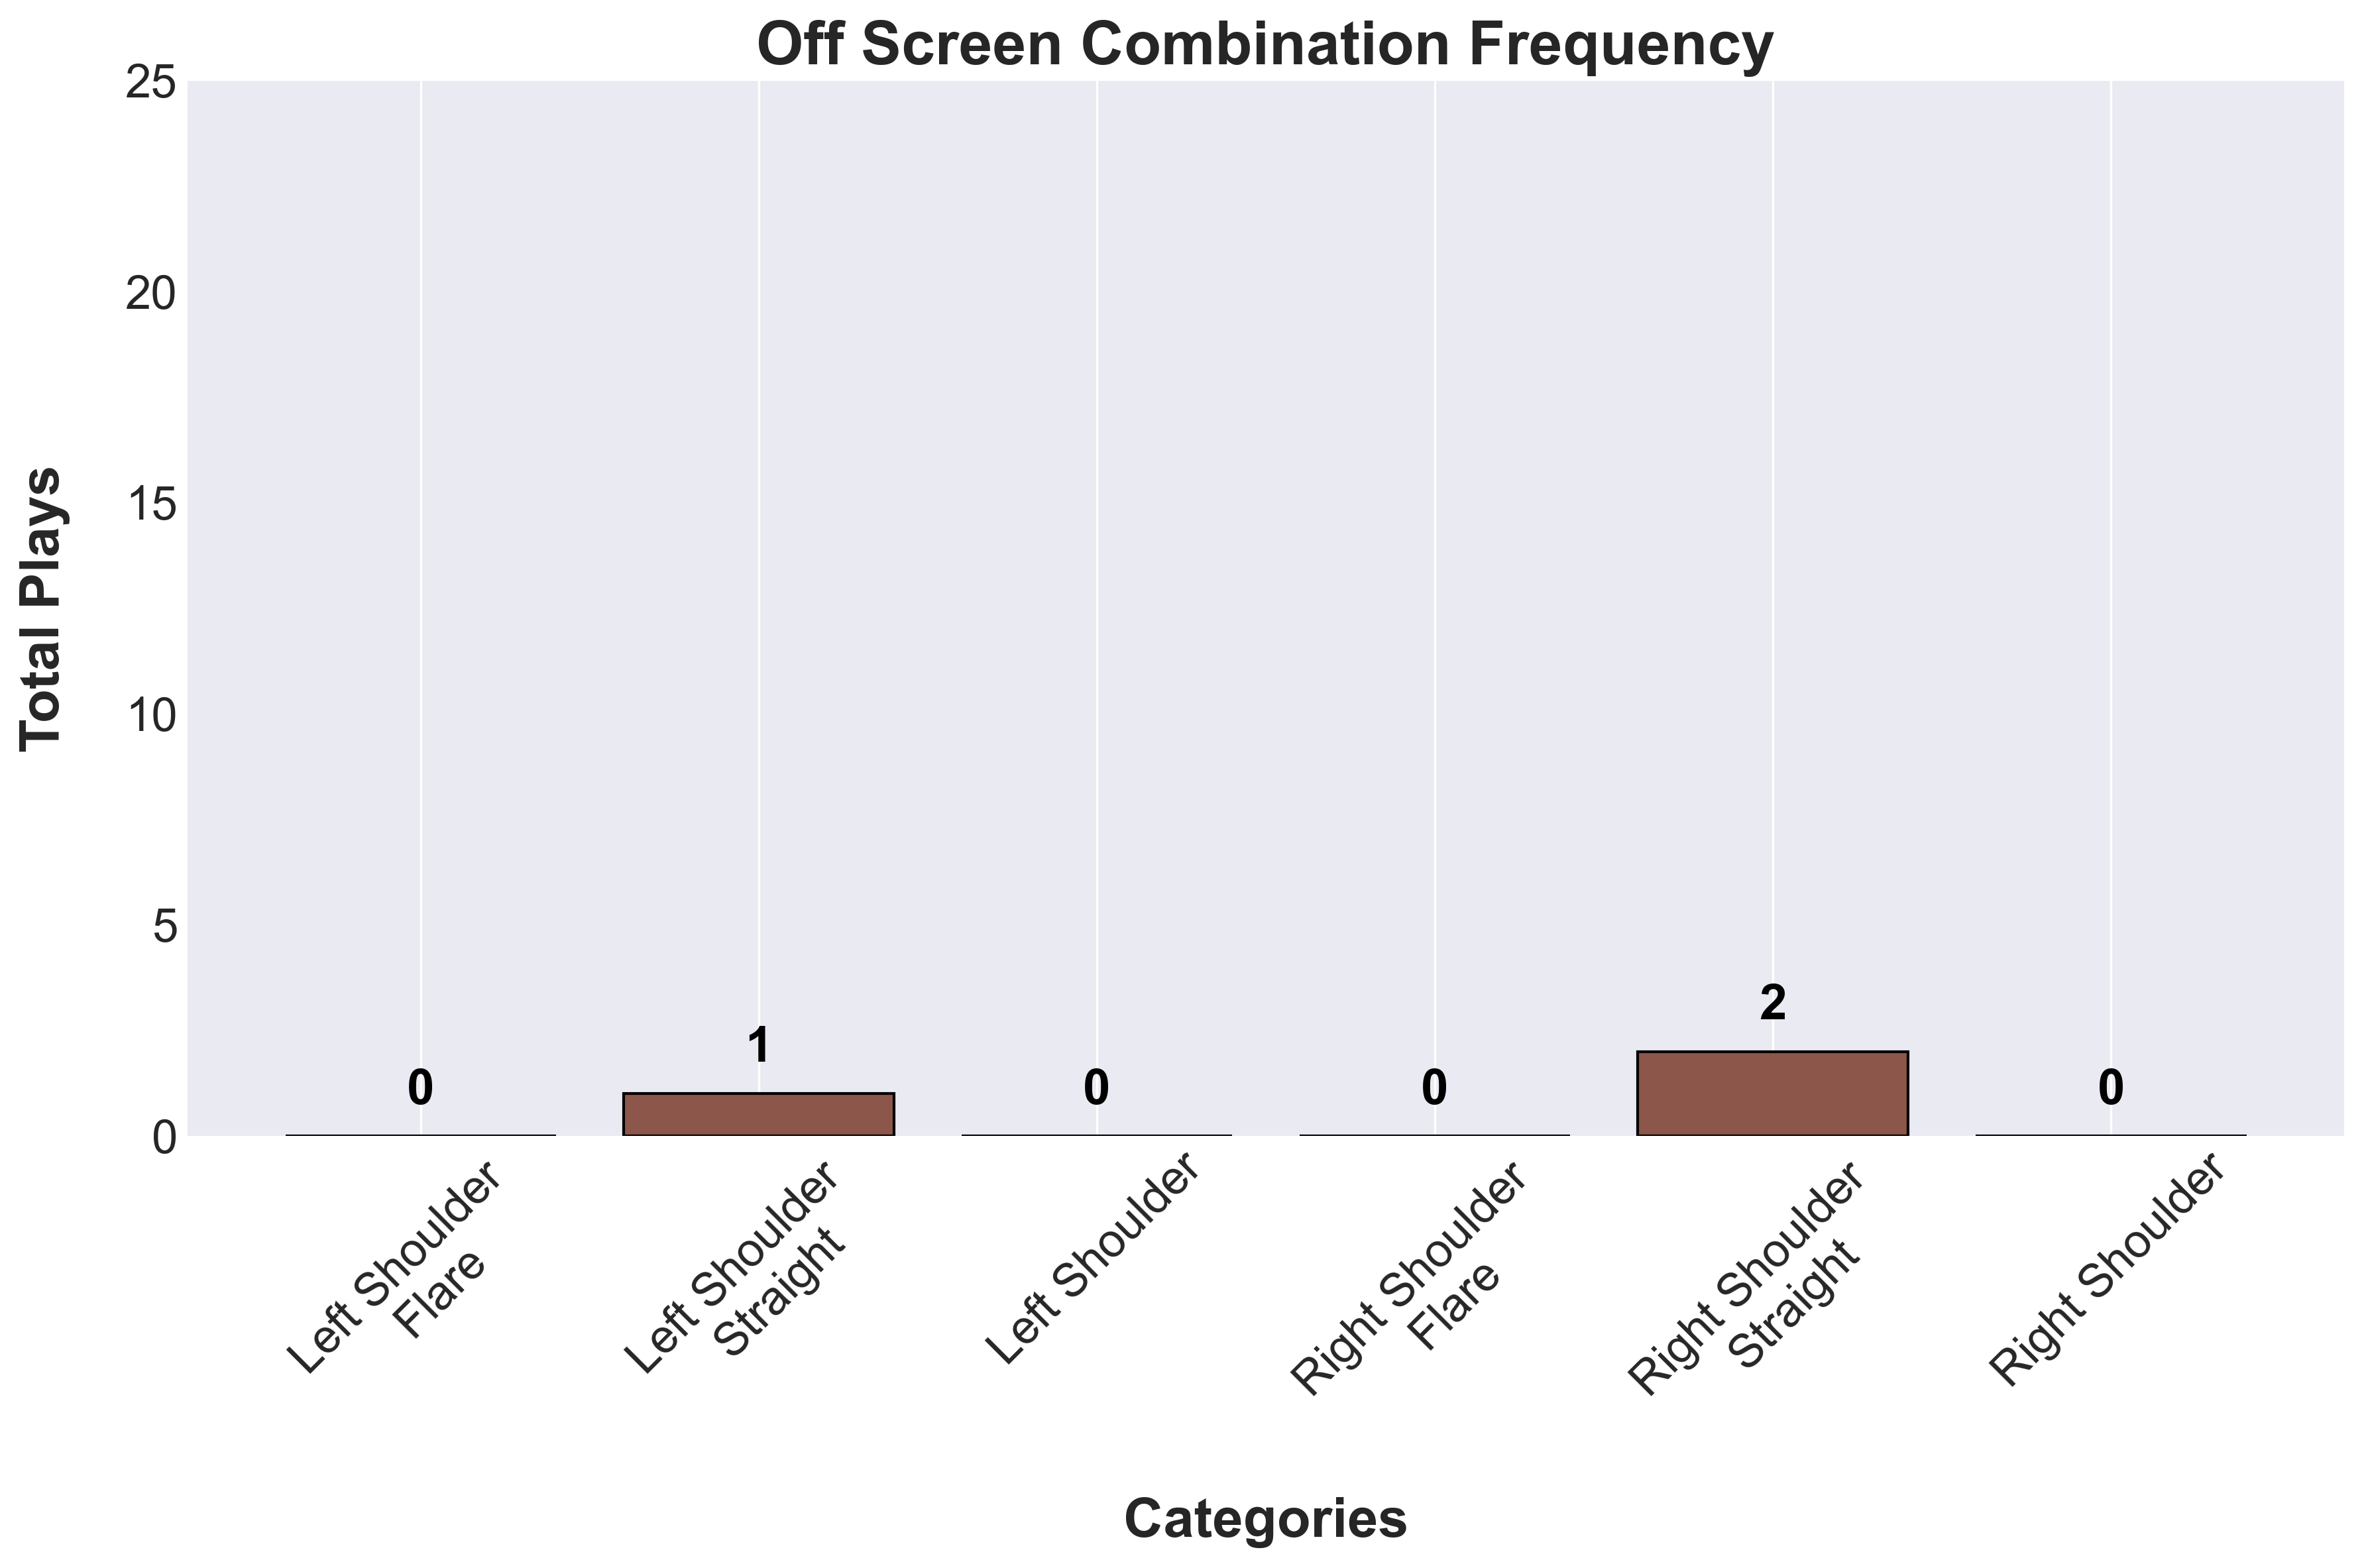
\includegraphics[width=\textwidth, height=.14\textheight]{images/OffScreen_Combination_Freq.png} % Adjust the width of the image to fit
    \end{minipage}
\end{table}

\vspace{-1em} % Add vertical space before the line (optional)
\hrule height 1pt width 1\textwidth % Adjust height and width
\vspace{1em} % Add vertical space after the line (optional)

\clearpage


% ----------------------
% Handoffs Visuals and Insights Section
% ----------------------
\subsection{Handoffs}
\begin{itemize}
    \item Opponent's handoff plays have a success rate of 60\%.
\end{itemize}

\vspace{1.25em} % Add vertical space before the line (optional)
\textbf{Key Notes on Handoff Tendencies}
\vspace{0.5em} % Add space between the title and the itemized list

\begin{itemize}
    \item Hand Offs make up x\% of players offensive load
    \vspace{0.3em} % Add space between the title and the itemized list
    \item Player is more likely to get pull up from 3 getting a handoff going left than going right
\end{itemize}

\vspace{1em} % Add vertical space before the line (optional)
\hrule height 1pt width 1\textwidth % Adjust height and width
\vspace{0em} % Add vertical space after the line (optional)

\subsubsection{Hand Off Shot Statistics}

% All Hand Off Statistics Table w/ room for insights
\begin{table}[H]
    \centering
    \begin{minipage}[t]{0.6\textwidth} % Left side (table) takes 85% of the width
        %\flushright
        \centering % Centering the title and the table
        \text{Total Hand Off Shot Statistics} % Title above the table in bold
        \vskip .25em % Adds vertical space between title and table
        \scalebox{.85}{ % Scale the entire table down by half
            \scriptsize % Reduce the font size
            \begin{tabular}{
            >{\centering\arraybackslash}p{.75cm} 
            >{\centering\arraybackslash}p{.5cm} 
            >{\centering\arraybackslash}p{.5cm} 
            >{\centering\arraybackslash}p{.5cm}
            >{\centering\arraybackslash}p{.5cm} 
            >{\centering\arraybackslash}p{.5cm} 
            >{\centering\arraybackslash}p{.5cm} 
            >{\centering\arraybackslash}p{.5cm}
            >{\centering\arraybackslash}p{.5cm} 
            >{\centering\arraybackslash}p{.5cm}
            >{\centering\arraybackslash}p{.75cm}
            >{\centering\arraybackslash}p{.5cm} 
            >{\centering\arraybackslash}p{.5cm}}% Adjust column widths
            \toprule
            \textbf{Plays} &
            \textbf{3PA} &
            \textbf{3PM} &
            \textbf{3P\%} & 
            \textbf{2PA} & 
            \textbf{2PM} & 
            \textbf{2P\%} & 
            \textbf{MiA} & 
            \textbf{MiM} &
            \textbf{Mi\%} &
            \textbf{EFG\%} &
            \textbf{TO} &
            \textbf{Foul} \\
            \midrule
            
                
                    18 & 2 & 1 &
                    - & 
                    13 & 7 &
                    - &
                    2 & 0 &
                    - &
                    - &
                    2 & 1 \\
                
            
                
            
                
            
                
            
                
            
                
            
                
            
                
            
                
            
                
            
                
            
                
            
                
            
                
            

            \bottomrule
            \end{tabular}
        }
    \end{minipage}
\end{table}

\vspace{0em} % Add vertical space before the line (optional)
%\hrule height 1pt width 1\textwidth % Adjust height and width
\vspace{-1em} % Add vertical space after the line (optional)

% Handoffs for shooting going Left vs Right
\begin{table}[H]
    \raisebox{3em}{ % Adjust this value to shift the tables vertically
    \begin{minipage}[t]{0.6\textwidth} % Left side (table) takes 85% of the width
        \flushleft
        \centering % Centering the title and the table
        \text{BH Hand Off Direction/Location Statistics} % Title above the table in bold
        \vskip .25em % Adds vertical space between title and table
        \scalebox{.6}{ % Scale the entire table down by half
            \renewcommand{\arraystretch}{1.4} % Adjust the number to increase or decrease row spacing
            \begin{tabular}{
            >{\centering\arraybackslash}p{1.75cm} 
            >{\centering\arraybackslash}p{.75cm} 
            >{\centering\arraybackslash}p{.75cm} 
            >{\centering\arraybackslash}p{.75cm} 
            >{\centering\arraybackslash}p{.75cm}
            >{\centering\arraybackslash}p{.75cm} 
            >{\centering\arraybackslash}p{.75cm} 
            >{\centering\arraybackslash}p{.75cm} 
            >{\centering\arraybackslash}p{.75cm}
            >{\centering\arraybackslash}p{.75cm} 
            >{\centering\arraybackslash}p{.75cm}
            >{\centering\arraybackslash}p{.75cm}
            >{\centering\arraybackslash}p{.75cm} 
            >{\centering\arraybackslash}p{.75cm}}% Adjust column widths
            \toprule
            {\scriptsize \textbf{PlayType}} &
            {\scriptsize \textbf{Plays}} &
            {\scriptsize \textbf{3PA}} &
            {\scriptsize \textbf{3PM}} &
            {\scriptsize \textbf{3P\%}} & 
            {\scriptsize \textbf{2PA}} & 
            {\scriptsize \textbf{2PM}} & 
            {\scriptsize \textbf{2P\%}} & 
            {\scriptsize \textbf{MiA}} & 
            {\scriptsize \textbf{MiM}} &
            {\scriptsize \textbf{Mi\%}} &
            {\scriptsize \textbf{EFG\%}} &
            {\scriptsize \textbf{TO}} &
            {\scriptsize \textbf{Foul}} \\
            \midrule
            
                
            
                
            
                
                    Left & 4 & 1 & 0 &
                    - & 
                    3 & 1 &
                    - &
                    1 & 0 &
                    - &
                    - &
                    0 & 0 \\
                
            
                
                    Right & 7 & 1 & 1 &
                    - & 
                    5 & 3 &
                    - &
                    1 & 0 &
                    - &
                    - &
                    1 & 0 \\
                
            
                
                    Top & 7 & 0 & 0 &
                    - & 
                    5 & 3 &
                    - &
                    0 & 0 &
                    - &
                    - &
                    1 & 1 \\
                
            
                
            
                
            
                
            
                
            
                
            
                
            
                
            
                
            
                
            

            \bottomrule
        \end{tabular}
        } % End of \scalebox
    \end{minipage}
    } % End of raisebox, closing the adjustment
    \hfill % This adds some flexible space between the table and the image
    \begin{minipage}[c]{0.35\textwidth} % Right side (image) takes 10% of the width
        \flushright
        \includegraphics[width=\textwidth, height=.14\textheight]{images/HandOff_Direction_Freq.png} % Adjust the width of the image to fit
    \end{minipage}
\end{table}

\vspace{-1em} % Add vertical space before the line (optional)
%\hrule height 1pt width 1\textwidth % Adjust height and width
\vspace{-1em} % Add vertical space after the line (optional)

% Hand Off Type Statistics
\begin{table}[H]
    \raisebox{3.5em}{ % Adjust this value to shift the tables vertically
    \begin{minipage}[t]{0.6\textwidth} % Left side (table) takes 85% of the width
        \flushleft
        \centering % Centering the title and the table
        \text{Hand Off Type Statistics} % Title above the table in bold
        \vskip .25em % Adds vertical space between title and table
        \scalebox{.6}{ % Scale the entire table down by half
            \renewcommand{\arraystretch}{1.4} % Adjust the number to increase or decrease row spacing
            \begin{tabular}{
            >{\centering\arraybackslash}p{1.75cm} 
            >{\centering\arraybackslash}p{.75cm} 
            >{\centering\arraybackslash}p{.75cm} 
            >{\centering\arraybackslash}p{.75cm} 
            >{\centering\arraybackslash}p{.75cm}
            >{\centering\arraybackslash}p{.75cm} 
            >{\centering\arraybackslash}p{.75cm} 
            >{\centering\arraybackslash}p{.75cm} 
            >{\centering\arraybackslash}p{.75cm}
            >{\centering\arraybackslash}p{.75cm} 
            >{\centering\arraybackslash}p{.75cm}
            >{\centering\arraybackslash}p{.75cm}
            >{\centering\arraybackslash}p{.75cm} 
            >{\centering\arraybackslash}p{.75cm}}% Adjust column widths
            \toprule
            {\scriptsize \textbf{PlayType}} &
            {\scriptsize \textbf{Plays}} &
            {\scriptsize \textbf{3PA}} &
            {\scriptsize \textbf{3PM}} &
            {\scriptsize \textbf{3P\%}} & 
            {\scriptsize \textbf{2PA}} & 
            {\scriptsize \textbf{2PM}} & 
            {\scriptsize \textbf{2P\%}} & 
            {\scriptsize \textbf{MiA}} & 
            {\scriptsize \textbf{MiM}} &
            {\scriptsize \textbf{Mi\%}} &
            {\scriptsize \textbf{EFG\%}} &
            {\scriptsize \textbf{TO}} &
            {\scriptsize \textbf{Foul}} \\
            \midrule
            
                
            
                
            
                
            
                
            
                
            
                
            
                
                    Stationary & 5 & 0 & 0 &
                    - & 
                    4 & 3 &
                    - &
                    0 & 0 &
                    - &
                    - &
                    0 & 1 \\
                
            
                
                    Dribble & 13 & 2 & 1 &
                    - & 
                    9 & 4 &
                    - &
                    2 & 0 &
                    - &
                    - &
                    2 & 0 \\
                
            
                
            
                
            
                
            
                
            
                
            
                
            


            \bottomrule
        \end{tabular}
        } % End of \scalebox
    \end{minipage}
    } % End of raisebox, closing the adjustment
    \hfill
    \begin{minipage}[c]{0.35\textwidth} % Right side (image) takes 10% of the width
        \flushright
        \includegraphics[width=\textwidth, height=.14\textheight]{images/HandOff_Type_Freq.png} % Adjust the width of the image to fit
    \end{minipage}
    
\end{table}

\vspace{-1em} % Add vertical space before the line (optional)
%\hrule height 1pt width 1\textwidth % Adjust height and width
\vspace{-1em} % Add vertical space after the line (optional)

% Hand Off Stats for Combination of Direction and Type Stats
\begin{table}[H]
    \raisebox{4.5em}{ % Adjust this value to shift the tables vertically
    \begin{minipage}[t]{0.6\textwidth} % Left side (table) takes 85% of the width
        \flushleft
        \centering % Centering the title and the table
        \text{Hand Off Combination Statistics} % Title above the table in bold
        \vskip .25em % Adds vertical space between title and table
        \scalebox{.55}{ % Scale the entire table down by half
            \renewcommand{\arraystretch}{1.4} % Adjust the number to increase or decrease row spacing
            \begin{tabular}{
            >{\centering\arraybackslash}p{4cm} 
            >{\centering\arraybackslash}p{.75cm} 
            >{\centering\arraybackslash}p{.75cm} 
            >{\centering\arraybackslash}p{.75cm} 
            >{\centering\arraybackslash}p{.75cm}
            >{\centering\arraybackslash}p{.75cm} 
            >{\centering\arraybackslash}p{.75cm} 
            >{\centering\arraybackslash}p{.75cm} 
            >{\centering\arraybackslash}p{.75cm}
            >{\centering\arraybackslash}p{.75cm} 
            >{\centering\arraybackslash}p{.75cm}
            >{\centering\arraybackslash}p{.75cm}
            >{\centering\arraybackslash}p{.75cm} 
            >{\centering\arraybackslash}p{.75cm}}% Adjust column widths
            \toprule
            {\scriptsize \textbf{PlayType}} &
            {\scriptsize \textbf{Plays}} &
            {\scriptsize \textbf{3PA}} &
            {\scriptsize \textbf{3PM}} &
            {\scriptsize \textbf{3P\%}} & 
            {\scriptsize \textbf{2PA}} & 
            {\scriptsize \textbf{2PM}} & 
            {\scriptsize \textbf{2P\%}} & 
            {\scriptsize \textbf{MiA}} & 
            {\scriptsize \textbf{MiM}} &
            {\scriptsize \textbf{Mi\%}} &
            {\scriptsize \textbf{EFG\%}} &
            {\scriptsize \textbf{TO}} &
            {\scriptsize \textbf{Foul}} \\
            \midrule
            
                
            
                
            
                
            
                
            
                
            
                
            
                
            
                
            
                
            
                
                    Right - Stationary & 1 & 0 & 0 &
                    - & 
                    1 & 1 &
                    - &
                    0 & 0 &
                    - &
                    - &
                    0 & 0 \\
                
            
                
                    Top - Stationary & 4 & 0 & 0 &
                    - & 
                    3 & 2 &
                    - &
                    0 & 0 &
                    - &
                    - &
                    0 & 1 \\
                
            
                
                    Left - Dribble & 4 & 1 & 0 &
                    - & 
                    3 & 1 &
                    - &
                    1 & 0 &
                    - &
                    - &
                    0 & 0 \\
                
            
                
                    Right - Dribble & 6 & 1 & 1 &
                    - & 
                    4 & 2 &
                    - &
                    1 & 0 &
                    - &
                    - &
                    1 & 0 \\
                
            
                
                    Top - Dribble & 3 & 0 & 0 &
                    - & 
                    2 & 1 &
                    - &
                    0 & 0 &
                    - &
                    - &
                    1 & 0 \\
                
            


            \bottomrule
        \end{tabular}
        } % End of \scalebox
    \end{minipage}
    } % End of raisebox, closing the adjustment
    \hfill % This adds some flexible space between the table and the image
    \begin{minipage}[c]{0.35\textwidth} % Right side (image) takes 10% of the width
        \flushright
        \includegraphics[width=\textwidth, height=.14\textheight]{images/HandOff_Combination_Freq.png} % Adjust the width of the image to fit
    \end{minipage}
\end{table}

\vspace{-1em} % Add vertical space before the line (optional)
\hrule height 1pt width 1\textwidth % Adjust height and width
\vspace{1em} % Add vertical space after the line (optional)

\clearpage


% ----------------------
% Iso Visuals and Insights Section
% ----------------------
\subsection{Iso}
\vspace{0.25em} % Add vertical space before the line (optional)
\textbf{Key Notes on Iso Tendencies}
\vspace{0.5em} % Add space between the title and the itemized list

\begin{itemize}
    \item Iso Plays make up x\% of players offensive load
    \vspace{0.3em} % Add space between the title and the itemized list
    \item Player is in the 35\% in scoring efficiency off cuts in the liberty league.
\end{itemize}

\vspace{1em} % Add vertical space after the line (optional)
\hrule height 1pt width 1\textwidth % Adjust height and width
\vspace{0em} % Add vertical space after the line (optional)

\subsubsection{General Iso Stats}
% All Cutter Statistics Table w/ room for insights
\begin{table}[H]
    \centering
    \begin{minipage}[t]{0.6\textwidth} % Left side (table) takes 85% of the width
        %\flushright
        \centering % Centering the title and the table
        \text{Total Iso Statistics} % Title above the table in bold
        \vskip .25em % Adds vertical space between title and table
        \scalebox{.85}{ % Scale the entire table down by half
            \scriptsize % Reduce the font size
            \begin{tabular}{
            >{\centering\arraybackslash}p{.75cm} 
            >{\centering\arraybackslash}p{.5cm} 
            >{\centering\arraybackslash}p{.5cm} 
            >{\centering\arraybackslash}p{.5cm}
            >{\centering\arraybackslash}p{.5cm} 
            >{\centering\arraybackslash}p{.5cm} 
            >{\centering\arraybackslash}p{.5cm} 
            >{\centering\arraybackslash}p{.5cm}
            >{\centering\arraybackslash}p{.5cm} 
            >{\centering\arraybackslash}p{.5cm}
            >{\centering\arraybackslash}p{.75cm}
            >{\centering\arraybackslash}p{.5cm} 
            >{\centering\arraybackslash}p{.5cm}}% Adjust column widths
            \toprule
            \textbf{Plays} &
            \textbf{3PA} &
            \textbf{3PM} &
            \textbf{3P\%} & 
            \textbf{2PA} & 
            \textbf{2PM} & 
            \textbf{2P\%} & 
            \textbf{MiA} & 
            \textbf{MiM} &
            \textbf{Mi\%} &
            \textbf{EFG\%} &
            \textbf{TO} &
            \textbf{Foul} \\
            \midrule
            


            \bottomrule
            \end{tabular}
        }
    \end{minipage}
\end{table}

\vspace{0em} % Add vertical space before the line (optional)
%\hrule height 1pt width 1\textwidth % Adjust height and width
\vspace{-1em} % Add vertical space after the line (optional)

% Iso Stats for Top vs Right vs Left 
\begin{table}[H]
    \raisebox{3em}{ % Adjust this value to shift the tables vertically
    \begin{minipage}[t]{0.6\textwidth} % Left side (table) takes 85% of the width
        \flushleft
        \centering % Centering the title and the table
        \text{Iso Direction/Location Statistics} % Title above the table in bold
        \vskip .25em % Adds vertical space between title and table
        \scalebox{.6}{ % Scale the entire table down by half
            \renewcommand{\arraystretch}{1.4} % Adjust the number to increase or decrease row spacing
            \begin{tabular}{
            >{\centering\arraybackslash}p{1.75cm} 
            >{\centering\arraybackslash}p{.75cm} 
            >{\centering\arraybackslash}p{.75cm} 
            >{\centering\arraybackslash}p{.75cm} 
            >{\centering\arraybackslash}p{.75cm}
            >{\centering\arraybackslash}p{.75cm} 
            >{\centering\arraybackslash}p{.75cm} 
            >{\centering\arraybackslash}p{.75cm} 
            >{\centering\arraybackslash}p{.75cm}
            >{\centering\arraybackslash}p{.75cm} 
            >{\centering\arraybackslash}p{.75cm}
            >{\centering\arraybackslash}p{.75cm}
            >{\centering\arraybackslash}p{.75cm} 
            >{\centering\arraybackslash}p{.75cm}}% Adjust column widths
            \toprule
            {\scriptsize \textbf{PlayType}} &
            {\scriptsize \textbf{Plays}} &
            {\scriptsize \textbf{3PA}} &
            {\scriptsize \textbf{3PM}} &
            {\scriptsize \textbf{3P\%}} & 
            {\scriptsize \textbf{2PA}} & 
            {\scriptsize \textbf{2PM}} & 
            {\scriptsize \textbf{2P\%}} & 
            {\scriptsize \textbf{MiA}} & 
            {\scriptsize \textbf{MiM}} &
            {\scriptsize \textbf{Mi\%}} &
            {\scriptsize \textbf{EFG\%}} &
            {\scriptsize \textbf{TO}} &
            {\scriptsize \textbf{Foul}} \\
            \midrule
            


            \bottomrule
        \end{tabular}
        } % End of \scalebox
    \end{minipage}
    } % End of raisebox, closing the adjustment
    \hfill % This adds some flexible space between the table and the image
    \begin{minipage}[c]{0.35\textwidth} % Right side (image) takes 10% of the width
        \flushright
        \includegraphics[width=\textwidth, height=.14\textheight]{images/IsoDirectionLocation_Freq.png} % Adjust the width of the image to fit
    \end{minipage}
\end{table}

\vspace{0em} % Add vertical space before the line (optional)
\hrule height 1pt width 1\textwidth % Adjust height and width
\vspace{1em} % Add vertical space after the line (optional)

\clearpage

% ----------------------
% Transition Visuals and Insights Section
% ----------------------
\subsection{Transition}
\vspace{0.25em} % Add vertical space before the line (optional)
\textbf{Key Notes on Iso Tendencies}
\vspace{0.5em} % Add space between the title and the itemized list

\begin{itemize}
    \item Transition Plays make up x\% of players offensive load
    \vspace{0.3em} % Add space between the title and the itemized list
    \item More Specifically, player is much more efficient getting out to left wing in transition vs the right wing in transition. 
\end{itemize}

\vspace{1em} % Add vertical space after the line (optional)
\hrule height 1pt width 1\textwidth % Adjust height and width
\vspace{0em} % Add vertical space after the line (optional)

\subsubsection{General Transition Stats}
% All Cutter Statistics Table w/ room for insights
\begin{table}[H]
    \centering
    \begin{minipage}[t]{0.6\textwidth} % Left side (table) takes 85% of the width
        %\flushright
        \centering % Centering the title and the table
        \text{Total Transition Statistics} % Title above the table in bold
        \vskip .25em % Adds vertical space between title and table
        \scalebox{.85}{ % Scale the entire table down by half
            \scriptsize % Reduce the font size
            \begin{tabular}{
            >{\centering\arraybackslash}p{.75cm} 
            >{\centering\arraybackslash}p{.5cm} 
            >{\centering\arraybackslash}p{.5cm} 
            >{\centering\arraybackslash}p{.5cm}
            >{\centering\arraybackslash}p{.5cm} 
            >{\centering\arraybackslash}p{.5cm} 
            >{\centering\arraybackslash}p{.5cm} 
            >{\centering\arraybackslash}p{.5cm}
            >{\centering\arraybackslash}p{.5cm} 
            >{\centering\arraybackslash}p{.5cm}
            >{\centering\arraybackslash}p{.75cm}
            >{\centering\arraybackslash}p{.5cm} 
            >{\centering\arraybackslash}p{.5cm}}% Adjust column widths
            \toprule
            \textbf{Plays} &
            \textbf{3PA} &
            \textbf{3PM} &
            \textbf{3P\%} & 
            \textbf{2PA} & 
            \textbf{2PM} & 
            \textbf{2P\%} & 
            \textbf{MiA} & 
            \textbf{MiM} &
            \textbf{Mi\%} &
            \textbf{EFG\%} &
            \textbf{TO} &
            \textbf{Foul} \\
            \midrule
            
                
            
                
                    69 & 5 & 1 &
                    - & 
                    37 & 22 &
                    - &
                    7 & 4 &
                    - &
                    - &
                    15 & 11 \\
                
            
                
            
                
            
                
            
                
            
                
            


            \bottomrule
            \end{tabular}
        }
    \end{minipage}
\end{table}

\vspace{0em} % Add vertical space before the line (optional)
%\hrule height 1pt width 1\textwidth % Adjust height and width
\vspace{-1em} % Add vertical space after the line (optional)

% Transitiom Stats for BH vs Leakouts vs Left Wing vs Right Wing vs Trailer
\begin{table}[H]
    \raisebox{4.5em}{ % Adjust this value to shift the tables vertically
    \begin{minipage}[t]{0.6\textwidth} % Left side (table) takes 85% of the width
        \flushleft
        \centering % Centering the title and the table
        \text{Transition Type Statistics} % Title above the table in bold
        \vskip .25em % Adds vertical space between title and table
        \scalebox{.58}{ % Scale the entire table down by half
            \renewcommand{\arraystretch}{1.4} % Adjust the number to increase or decrease row spacing
            \begin{tabular}{
            >{\centering\arraybackslash}p{2.5cm} 
            >{\centering\arraybackslash}p{.75cm} 
            >{\centering\arraybackslash}p{.75cm} 
            >{\centering\arraybackslash}p{.75cm} 
            >{\centering\arraybackslash}p{.75cm}
            >{\centering\arraybackslash}p{.75cm} 
            >{\centering\arraybackslash}p{.75cm} 
            >{\centering\arraybackslash}p{.75cm} 
            >{\centering\arraybackslash}p{.75cm}
            >{\centering\arraybackslash}p{.75cm} 
            >{\centering\arraybackslash}p{.75cm}
            >{\centering\arraybackslash}p{.75cm}
            >{\centering\arraybackslash}p{.75cm} 
            >{\centering\arraybackslash}p{.75cm}}% Adjust column widths
            \toprule
            {\scriptsize \textbf{PlayType}} &
            {\scriptsize \textbf{Plays}} &
            {\scriptsize \textbf{3PA}} &
            {\scriptsize \textbf{3PM}} &
            {\scriptsize \textbf{3P\%}} & 
            {\scriptsize \textbf{2PA}} & 
            {\scriptsize \textbf{2PM}} & 
            {\scriptsize \textbf{2P\%}} & 
            {\scriptsize \textbf{MiA}} & 
            {\scriptsize \textbf{MiM}} &
            {\scriptsize \textbf{Mi\%}} &
            {\scriptsize \textbf{EFG\%}} &
            {\scriptsize \textbf{TO}} &
            {\scriptsize \textbf{Foul}} \\
            \midrule
            
                
            
                
            
                
                    BH & 42 & 1 & 0 &
                    - & 
                    20 & 11 &
                    - &
                    4 & 2 &
                    - &
                    - &
                    11 & 10 \\
                
            
                
                    Leakouts & 3 & 0 & 0 &
                    - & 
                    2 & 2 &
                    - &
                    0 & 0 &
                    - &
                    - &
                    0 & 0 \\
                
            
                
                    Left Wing & 16 & 1 & 1 &
                    - & 
                    11 & 5 &
                    - &
                    2 & 1 &
                    - &
                    - &
                    3 & 1 \\
                
            
                
                    Right Wing & 8 & 3 & 0 &
                    - & 
                    4 & 4 &
                    - &
                    1 & 1 &
                    - &
                    - &
                    1 & 0 \\
                
            
                
                    Trailer & 4 & 4 & 2 &
                    - & 
                    0 & 0 &
                    - &
                    0 & 0 &
                    - &
                    - &
                    0 & 0 \\
                
            


            \bottomrule
        \end{tabular}
        } % End of \scalebox
    \end{minipage}
    } % End of raisebox, closing the adjustment
    \hfill % This adds some flexible space between the table and the image
    \begin{minipage}[c]{0.35\textwidth} % Right side (image) takes 10% of the width
        \flushright
        \includegraphics[width=\textwidth, height=.14\textheight]{images/Transition_Type_Freq.png} % Adjust the width of the image to fit
    \end{minipage}
\end{table}

\vspace{0em} % Add vertical space before the line (optional)
\hrule height 1pt width 1\textwidth % Adjust height and width
\vspace{1em} % Add vertical space after the line (optional)

\clearpage


%---------------------------------
% Conclusion Section
%---------------------------------
\section*{Conclusion}
This report provides a comprehensive look at how to defend Player X based on personalized statistics across multiple play types. By focusing on key weaknesses, such as spot-up defense and PNR efficiency, we can create a game plan that maximizes defensive success.

\end{document}